\documentclass[12pt,a4paper]{report}
\usepackage[utf8]{inputenc}
\usepackage[T1]{fontenc}
\usepackage[french]{babel}
\usepackage{geometry}
\geometry{margin=2.5cm, top=3cm}
\setlength{\headheight}{14.5pt}
\usepackage{graphicx}
% NOTE: Ajouter [draft] ci-dessus si les images PNG ne sont pas encore exportées :
% \usepackage[draft]{graphicx}
\usepackage{hyperref}
\usepackage{listings}
\usepackage{xcolor}
\usepackage{booktabs}
\usepackage{longtable}
\usepackage{float}
\usepackage{fancyhdr}
\usepackage{titlesec}
\usepackage{tocloft}
\usepackage{enumitem}
\usepackage{amsmath}
\usepackage{amssymb}
\usepackage{tikz}
\usepackage{pgfplots}
\pgfplotsset{compat=1.18}
\usetikzlibrary{shapes.geometric, arrows.meta, positioning, calc}
\usepackage{setspace}
\onehalfspacing

% Colors
\definecolor{stblue}{RGB}{26,35,126}
\definecolor{stlightblue}{RGB}{200,220,255}
\definecolor{storange}{RGB}{255,152,0}
\definecolor{stgreen}{RGB}{76,175,80}
\definecolor{stgray}{RGB}{200,200,200}
\definecolor{stred}{RGB}{210,60,60}
\definecolor{codebg}{RGB}{245,245,245}
\definecolor{codeframe}{RGB}{200,200,200}

\lstdefinelanguage{json}{
  basicstyle=\ttfamily\small,
  showstringspaces=false,
  breaklines=true,
  string=[s]"",
  stringstyle=\color{red!70!black},
  comment=[l]{//},
  morecomment=[s]{/*}{*/},
  commentstyle=\color{gray},
  morekeywords={true,false,null},
  keywordstyle=\color{blue}
}

% Code listing style
\lstset{
  backgroundcolor=\color{codebg},
  frame=single,
  rulecolor=\color{codeframe},
  basicstyle=\ttfamily\small,
  breaklines=true,
  keywordstyle=\color{blue},
  commentstyle=\color{gray},
  stringstyle=\color{red!70!black},
}

% Headers
\pagestyle{fancy}
\fancyhf{}
\fancyhead[L]{\leftmark}
\fancyhead[R]{PFE --- Chatbot STM32Cube}
\fancyfoot[C]{\thepage}

\hypersetup{
  colorlinks=true,
  linkcolor=stblue,
  urlcolor=blue!70!black,
  citecolor=stblue,
}

% Graphics path for diagrams and evaluation charts
\graphicspath{
  {../diagrams/presentation/exported/}
  {../diagrams/technical/exported/}
  {../../datasets/07_delivery/st_ready/evaluation_report/}
  {./figures/}
}

\begin{document}

%% ============================================================
%% TITLE PAGE
%% ============================================================
\begin{titlepage}
\centering
\vspace*{1cm}

{\Large \textbf{Université / École d'Ingénieur}}\\[0.3cm]
{\large Département Informatique / Génie Logiciel}\\[2cm]

{\Huge \textbf{Projet de Fin d'Études}}\\[0.5cm]
{\LARGE Rapport de Stage}\\[1.5cm]

\rule{\textwidth}{1pt}\\[0.5cm]
{\huge \textbf{Conception et Implémentation d'un Pipeline\\de Prétraitement Intelligent pour la\\Base de Connaissances STM32Cube}}\\[0.5cm]
\rule{\textwidth}{1pt}\\[2cm]

\begin{minipage}{0.45\textwidth}
\begin{flushleft}
\textbf{Réalisé par :}\\
Abir GHARBI
\end{flushleft}
\end{minipage}
\hfill
\begin{minipage}{0.45\textwidth}
\begin{flushright}
\textbf{Encadrant entreprise :}\\
{[Nom du tuteur ST]}\\[0.5cm]
\textbf{Encadrant académique :}\\
{[Nom du tuteur académique]}
\end{flushright}
\end{minipage}

\vfill

\textbf{Entreprise d'accueil :} STMicroelectronics\\
\textbf{Division :} AI \& Digital Tools\\[0.5cm]
\textbf{Année universitaire :} 2025--2026

\end{titlepage}

%% ============================================================
\chapter*{Remerciements}
\addcontentsline{toc}{chapter}{Remerciements}

Je tiens à exprimer ma sincère gratitude envers toute l'équipe STMicroelectronics pour leur accueil, leur encadrement et leur soutien tout au long de ce stage. Je remercie particulièrement [nom du tuteur] pour sa disponibilité et ses conseils avisés.

\newpage
\tableofcontents
\newpage
\listoffigures
\newpage

%% ============================================================
%% INTRODUCTION GÉNÉRALE (hors chapitres)
%% ============================================================
\chapter*{Introduction Générale}
\addcontentsline{toc}{chapter}{Introduction Générale}
\markboth{Introduction Générale}{Introduction Générale}

Le développement de systèmes embarqués basés sur les microcontrôleurs STM32 de STMicroelectronics est un domaine en constante évolution, où les ingénieurs font face quotidiennement à des problèmes techniques complexes : bugs de drivers, comportements inattendus des périphériques, incompatibilités entre versions firmware, configurations matérielles spécifiques. Pour résoudre ces problèmes, ils doivent aujourd'hui parcourir manuellement des milliers d'issues GitHub, des centaines de fichiers de documentation, et des dizaines de Release Notes répartis sur plus de 200 dépôts --- un processus lent, fragmenté et inefficace.

Ce projet de fin d'études, réalisé au sein de l'équipe \textbf{Technical Marketing and Application Support} de la division Microcontrôleurs (MCD) du site STMicroelectronics de Tunis, propose une solution à cette problématique : la conception et l'implémentation d'un \textbf{pipeline de prétraitement intelligent} qui transforme automatiquement les données brutes des dépôts GitHub STM32Cube en une base de connaissances structurée. Cette base alimente un chatbot IA spécialisé (``ST GitHub Analyzer'') déployé sur la plateforme interne ST ChatGPT, capable de fournir des diagnostics précis, sourcés et actionnables aux ingénieurs.

Le pipeline couvre les \textbf{25 séries} de la famille STM32 (13 en production, 12 configurées) et produit 4 types d'artefacts complémentaires : issues structurées, fichiers documentés, resolver cases (chaînes issue→PR→commit) et diagnostic cards (analyses de pannes structurées). Un enrichissement IA multi-modal par Alfred Vision rend le contenu visuel (captures d'écran, figures PDF) exploitable par la recherche.

Les résultats démontrent une \textbf{amélioration nette de la pertinence} par rapport à un LLM générique sur les questions techniques STM32, avec un Quality Index atteignant 94/100 sur la série pilote H7 grâce aux Diagnostic Cards.

Ce rapport est organisé en \textbf{cinq chapitres}, encadrés par la présente introduction générale et une conclusion générale :
\begin{itemize}
  \item \textbf{Chapitre 1 --- Contexte Général du Projet} : présentation de l'entreprise d'accueil, du site de Tunis, de la division Microcontrôleurs et de l'équipe d'accueil, de l'écosystème STM32/GitHub, de la problématique, des objectifs et des contributions
  \item \textbf{Chapitre 2 --- État de l'Art et Fondements Théoriques} : le paradigme RAG, les enjeux du preprocessing pour une KB, la similarité TF-IDF, Alfred Vision, le positionnement par rapport aux solutions existantes, et la notion générale de pipeline de preprocessing (étapes canoniques, métriques, patterns)
  \item \textbf{Chapitre 3 --- Analyse des Besoins et Conception} : identification des acteurs, besoins fonctionnels et non fonctionnels, contraintes de conception, choix méthodologique (Scrum adapté et CRISP-DM --- avec une justification comparative face aux méthodologies alternatives), contraintes de la plateforme de retrieval et architecture cible
  \item \textbf{Chapitre 4 --- Réalisation et Implémentation} : les 7 stages du pipeline (ingestion à delivery), l'enrichissement Alfred Vision, puis la configuration de la persona sur la plateforme ST ChatGPT et l'automatisation CI/CD
  \item \textbf{Chapitre 5 --- Résultats et Évaluation} : métriques par stage, confiance Alfred, évolution incrémentale du Quality Index, et étude comparative Alfred générique vs Persona KB
\end{itemize}

\newpage

%% ============================================================
\chapter{Contexte Général du Projet}
\label{chap:contexte}
%% ============================================================

\section*{Introduction}

Ce chapitre présente l'entreprise d'accueil et le cadre dans lequel ce projet de fin d'études a été mené, avant d'exposer l'écosystème STM32/GitHub, la problématique précise à laquelle répond le projet, ses objectifs et ses contributions. Nous décrivons successivement STMicroelectronics à l'échelle mondiale, le site de Tunis, la division Microcontrôleurs (MCD) et l'équipe Technical Marketing and Application Support --- et en son sein l'équipe Maintenance et Validation --- qui a accueilli ce travail. Cette présentation constitue le socle sur lequel s'appuiera le chapitre suivant pour introduire les fondements théoriques du projet.

\section{Présentation de l'Entreprise}
\label{sec:st_presentation}

\subsection{Présentation Générale}

\textbf{STMicroelectronics} est une entreprise mondiale de semi-conducteurs dédiée à l'amélioration de la vie quotidienne grâce à des solutions électroniques innovantes \cite{stm32}. Avec l'un des portefeuilles de produits les plus étendus de l'industrie, ST dessert plus de 200\,000 clients dans le monde, réalisant un chiffre d'affaires net de 13,27 milliards USD en 2024 \cite{st_annual_report}.

L'entreprise a été fondée en juin 1987 sous le nom de \textbf{SGS-THOMSON Microelectronics}, suite à la fusion de SGS Microelettronica (Italie) et de Thomson Semiconductors (France). Le nom ``STMicroelectronics'' a été officiellement adopté en mai 1998. Avec plus de 80 bureaux commerciaux et 14 sites de fabrication principaux à travers le monde, l'entreprise emploie plus de 50\,000 personnes \cite{st_annual_report}.

% Figure : Logo ST (à exporter depuis draw.io)
\begin{figure}[H]
\centering
\fbox{\textit{[Logo STMicroelectronics --- exporter depuis draw.io]}}
\caption{Logo officiel de STMicroelectronics}
\label{fig:st_logo}
\end{figure}

\subsection{Vision et Marchés}

STMicroelectronics a fait de l'innovation technologique une priorité stratégique depuis plus de 25 ans. L'entreprise réalise des investissements orientés marché dans le développement technologique, avec l'objectif de commercialiser des innovations de pointe créant une valeur immédiate pour ses clients. Aujourd'hui, ST livre des produits toujours plus petits, plus rapides, plus économes en énergie et dotés de nouvelles fonctionnalités.

Portée par une culture mondiale de \textit{lean manufacturing}, ST adresse \textbf{trois marchés principaux} :
\begin{itemize}
  \item \textbf{Automobile} (37\%) : capteurs, microcontrôleurs, gestion de puissance pour véhicules électriques et autonomes
  \item \textbf{Industriel} (30\%) : automatisation, contrôle moteur, IoT industriel, smart grid
  \item \textbf{Électronique personnelle} (20\%) : smartphones, wearables, audio, gaming
  \item \textbf{Communications et équipements} (13\%) : infrastructure réseau, serveurs
\end{itemize}

ST propose des modèles d'engagement allant des systèmes embarqués spécifiques à l'application jusqu'aux produits standard spécialisés (ASSP).

\subsection{STMicroelectronics Tunis}
\label{sec:st_tunis}

Le site \textbf{ST Tunis}, situé dans le \textbf{Technopark El Ghazela}, a débuté ses opérations en 2001 avec neuf ingénieurs. Aujourd'hui, il compte plus de \textbf{200 employés} travaillant dans les domaines du design, des outils, des applications, de la qualité et du support \cite{st_annual_report}. Le site participe à chaque étape, depuis la conception initiale de nouveaux circuits jusqu'à la vérification finale de leur fonctionnalité avant la production de masse.

\section{Division Microcontrôleurs (MCD)}
\label{sec:mcd}

La \textbf{Microcontroller Division (MCD)} est dédiée à la conception de microcontrôleurs, de plateformes de démonstration et de solutions pour les applications grand public. Elle est responsable du développement de drivers et de logiciels embarqués --- en particulier la validation et le développement des bibliothèques et firmware qui pilotent les microcontrôleurs ST. La division couvre l'ensemble du cycle de vie du firmware : conception initiale, portage entre séries, validation fonctionnelle, maintenance corrective et support aux clients externes.

La Figure~\ref{fig:st-site-org} présente l'organisation de la MCD sur le site de Tunis. L'équipe \textbf{Maintenance} (mise en évidence) est l'équipe d'accueil de ce projet de fin d'études.

\begin{figure}[H]
\centering
\fbox{\parbox{0.7\textwidth}{\centering\vspace{2.2cm}\textit{[Organigramme MCD --- ST Tunis\\à exporter depuis draw.io : \texttt{Figures/chapter1/st-site-organization.pdf}]}\vspace{2.2cm}}}
\caption{Structure organisationnelle de la division Microcontrôleurs (MCD) au site ST Tunis. L'équipe Maintenance (mise en évidence) est l'équipe d'accueil de ce projet.}
\label{fig:st-site-org}
\end{figure}

\section{Équipe d'Accueil : Technical Marketing and Application Support}
\label{sec:equipe_accueil}

Ce projet a été réalisé au sein de l'équipe \textbf{Technical Marketing and Application Support}, rattachée à la MCD sur le site de Tunis. Cette équipe assure la jonction entre les équipes de conception (design), les clients externes utilisant les microcontrôleurs STM32, et les processus internes de qualité et d'industrialisation. Elle comprend deux sous-équipes complémentaires :

\begin{itemize}
  \item \textbf{L'équipe GitHub} : assure le support client via les dépôts GitHub publics de STMicroelectronics, publie les mises à jour des drivers HAL, et maintient les projets d'exemples pour faciliter le développement d'applications basées sur les microcontrôleurs STM32.

  \item \textbf{L'équipe Maintenance et Validation} : garantit la satisfaction client par la maintenance des bugs et la validation fonctionnelle des microcontrôleurs fabriqués et de leurs versions HAL associées. Cette équipe représente la jonction entre les processus de conception logicielle/matérielle et l'industrialisation. \textbf{C'est au sein de cette équipe que le présent projet de fin d'études a été réalisé.}
\end{itemize}

C'est dans ce contexte opérationnel que le besoin d'un \textbf{chatbot IA spécialisé STM32} a émergé : face au volume croissant d'issues GitHub (plusieurs milliers par an, répartis sur 200+ dépôts) et à la richesse inexploitée de ces données, l'équipe Maintenance et Validation a identifié l'opportunité d'automatiser le support de premier niveau par un pipeline intelligent de prétraitement alimentant une base de connaissances structurée. Les sections suivantes détaillent cet écosystème, la problématique précise qui en découle, ainsi que les objectifs et contributions du projet.

\section{L'Écosystème STM32 et les Dépôts GitHub}
\label{sec:ecosysteme}

\textit{\small\textbf{\textcolor{stblue}{Phase CRISP-DM :}} Data Understanding (analyse des sources de données brutes), avec un ancrage en Business Understanding pour le cadrage de l'écosystème STM32.}\par\smallskip

Au cœur de l'offre de ST se trouve la famille \textbf{STM32}, une gamme de microcontrôleurs basés sur les cœurs ARM Cortex-M (M0, M0+, M3, M4, M7, M33, M55) et Cortex-A. Lancée en 2007, la famille STM32 compte aujourd'hui plus de \textbf{1\,500 références} regroupées en plus de 30 séries, chacune ciblant un profil d'application spécifique :

\begin{longtable}{p{2.5cm}p{3cm}p{7.5cm}}
\toprule
\textbf{Série} & \textbf{Cœur} & \textbf{Cible applicative} \\
\midrule
STM32F0/F1/F2 & Cortex-M0/M3 & Entrée de gamme, migration depuis 8-bit \\
STM32F3/F4 & Cortex-M4F & Applications signal mixte, contrôle moteur, audio \\
STM32F7 & Cortex-M7 & Haute performance, graphisme, connectivité \\
STM32G0/G4 & Cortex-M0+/M4 & Nouvelle génération mainstream, efficacité énergétique \\
STM32H5/H7/H7RS & Cortex-M33/M7 & Ultra-haute performance, dual-core, temps réel \\
STM32L0/L1/L4/L5 & Cortex-M0+/M3/M4/M33 & Ultra-basse consommation, IoT, wearables \\
STM32U0/U3/U5 & Cortex-M0+/M33 & Ultra-basse consommation nouvelle génération \\
STM32WB/WBA/WL & Cortex-M4+M0/M33 & Connectivité sans fil (BLE, Thread, LoRa, Sub-GHz) \\
STM32N6 & Cortex-M55+NPU & IA embarquée, vision par ordinateur \\
\bottomrule
\end{longtable}

Pour chaque série, ST fournit un \textbf{Firmware Package} complet sous le nom \textbf{STM32Cube}, comprenant :
\begin{itemize}
  \item Le \textbf{HAL} (Hardware Abstraction Layer) : couche d'abstraction portable entre séries
  \item Les \textbf{drivers LL} (Low-Layer) : accès registre optimisé pour la performance
  \item Les \textbf{BSP} (Board Support Packages) : drivers spécifiques aux cartes de développement (NUCLEO, Discovery, Eval)
  \item Les \textbf{CMSIS Device Headers} : définitions de registres ARM standardisées
  \item Des \textbf{Middlewares} : FreeRTOS, LwIP, FatFs, USB, TouchGFX, LoRaWAN
  \item Des \textbf{exemples d'application} : projets prêts à compiler par board et par IDE
\end{itemize}

\subsection{Les Dépôts GitHub STMicroelectronics}

Depuis 2019, STMicroelectronics publie l'intégralité de ses firmware packages STM32Cube en open source sur GitHub (\texttt{github.com/STMicroelectronics}). Cette présence GitHub représente un écosystème considérable :

\begin{itemize}
  \item \textbf{25 dépôts principaux} (un par série MCU : \texttt{STM32CubeH7}, \texttt{STM32CubeF4}, etc.)
  \item \textbf{200+ sous-dépôts} pour les drivers individuels (\texttt{stm32h7xx-hal-driver}, \texttt{stm32f4xx-nucleo-bsp}, \texttt{cmsis\_device\_h7}, etc.)
  \item \textbf{Des milliers d'issues} ouvertes par la communauté (bug reports, questions d'utilisation, demandes de fonctionnalités)
  \item \textbf{Des centaines de Pull Requests} avec des corrections de code et des discussions techniques
  \item De la \textbf{documentation technique} embarquée : Release Notes (HTML), README (Markdown), documentation PDF
\end{itemize}

Ce projet porte sur les \textbf{25 séries} de la famille STM32 : \textbf{13 séries en production} (C0, F0, F1, F2, F3, F4, F7, G0, H5, H7, H7RS, U5, WL) couvrant 47 dépôts et \textbf{12 séries supplémentaires} configurées et prêtes au déploiement (G4, L0, L1, L4, L5, N6, U0, U3, WB, WB0, WBA, WL3). La couverture totale cible est de \textbf{25 séries MCU} avec plus de 200 sous-dépôts associés.

\section{Problématique}
\label{sec:problematique}

\textit{\small\textbf{\textcolor{stblue}{Phase CRISP-DM :}} Business Understanding (formulation du problème métier et des objectifs de support).}\par\smallskip

Les ingénieurs STM32 --- qu'ils soient internes à ST ou clients --- rencontrent quotidiennement des problèmes techniques lors du développement firmware : bugs HAL, comportements inattendus des périphériques, incompatibilités entre versions, configurations complexes. Pour résoudre ces problèmes, ils doivent aujourd'hui parcourir manuellement les ressources disponibles, un processus qui souffre de quatre limitations majeures :

\begin{enumerate}
  \item \textbf{Volume et dispersion} : les données sont réparties sur plus de 200 dépôts GitHub, totalisant des milliers d'issues, des centaines de PRs et des dizaines de milliers de fichiers source. Trouver l'information pertinente revient à chercher une aiguille dans une botte de foin numérique.
  
  \item \textbf{Bruit et hétérogénéité} : le contenu des issues mélange du texte technique utile avec du bruit considérable --- templates vides, messages automatiques de bots GitHub, discussions hors-sujet, doublons, markdown malformé. Les fichiers source contiennent des licences volumineuses (30\% du texte pour certains fichiers) et les headers CMSIS dépassent 1,7~Mo de définitions bit-à-bit inutiles pour le diagnostic.
  
  \item \textbf{Fragmentation des connaissances} : la résolution d'un bug implique souvent de recouper une issue, une PR avec sa discussion, un commit dans un sous-dépôt différent, et une Release Note qui documente le correctif. Ces liens ne sont pas toujours explicites dans GitHub et nécessitent une investigation manuelle fastidieuse.
  
  \item \textbf{Opacité du contenu visuel} : de nombreuses issues contiennent des captures d'écran (erreurs IDE STM32CubeIDE, oscillogrammes, configurations CubeMX, schémas de câblage) qui portent une information diagnostique critique mais sont totalement invisibles pour la recherche textuelle. De même, les Release Notes PDF contiennent des figures techniques non indexables.
\end{enumerate}

\textbf{La question centrale de ce projet} est donc : \textit{comment transformer cette masse de données brutes, hétérogènes et fragmentées en une base de connaissances structurée, exploitable par un chatbot IA capable de fournir des diagnostics précis, sourcés et actionnables aux ingénieurs STM32 ?}

\subsection{Critique de l'Existant}

Avant ce projet, les solutions disponibles présentaient des limitations significatives :

\begin{longtable}{p{3.5cm}p{5.5cm}p{4.5cm}}
\toprule
\textbf{Solution existante} & \textbf{Limitation principale} & \textbf{Impact utilisateur} \\
\midrule
Recherche GitHub native & Recherche textuelle brute, pas de filtrage par composant, layer ou sévérité & L'ingénieur parcourt 50+ issues sans garantie de trouver la bonne \\
Alfred (LLM ST) & Connaissances génériques, aucun accès aux issues GitHub spécifiques & Conseils généraux sans root cause précise ni traçabilité \\
Stack Overflow & Communauté large mais non spécifique ST, pas de traçabilité vers les correctifs officiels & Solutions non vérifiées, souvent obsolètes ou inapplicables \\
Documentation PDF & Non indexable, figures opaques, pas de lien avec les bugs connus & L'ingénieur ne peut pas corréler son problème avec les bugs documentés \\
Support direct (email/forum) & Temps de réponse de 48h à 2 semaines & Blocage du développement client \\
\bottomrule
\end{longtable}

\textbf{Constat quantifié} : Sur un benchmark de 20 questions techniques couvrant 5 séries MCU, Alfred générique obtient un score de 116/200 (58\%) tandis que notre solution avec Knowledge Base obtient 161/200 (80,5\%), soit un \textbf{gain de +39\%} en pertinence, actionnabilité et traçabilité (cf. Section~\ref{sec:etude_comparative} pour le détail de l'étude).

\section{Objectifs du Projet}
\label{sec:objectifs}

Les objectifs de ce projet de fin d'études sont les suivants :

\begin{enumerate}
  \item \textbf{Concevoir} un pipeline de prétraitement automatisé capable d'ingérer les données brutes depuis l'API GitHub, de les nettoyer, enrichir et structurer pour un système RAG
  \item \textbf{Implémenter} les 7 étapes du pipeline (ingestion, nettoyage V1+V3, enrichissement NLP, similarité TF-IDF, chunking, validation, delivery) avec une architecture modulaire et rejouable
  \item \textbf{Déployer} un chatbot IA spécialisé STM32 sur la plateforme ST ChatGPT, alimenté par la Knowledge Base générée par le pipeline
  \item \textbf{Évaluer} la qualité du système de bout en bout via un Quality Index sur 52 questions et une étude comparative avec Alfred générique
  \item \textbf{Automatiser} la mise à jour continue via CI/CD (GitHub Actions) et des scripts d'orchestration
  \item \textbf{Industrialiser} la solution pour couvrir l'intégralité des 25 séries STM32
\end{enumerate}

\section{Contributions Techniques Originales}
\label{sec:contributions}

\begin{enumerate}
  \item \textbf{Pipeline modulaire 7 stages} rejouable indépendamment par étape avec artefacts JSON traçables
  \item \textbf{Nettoyage V3 par type} : routage intelligent avec réduction de 96\% sur les headers CMSIS et 33\% sur le HTML
  \item \textbf{Filtre CMSIS intelligent} ne conservant que les sections à valeur diagnostique (IRQ, base addresses, TypeDef)
  \item \textbf{4 types d'artefacts delivery} complémentaires : issues, files, resolver cases, diagnostic cards
  \item \textbf{Heuristiques NLP domain-specific} pour la classification STM32 (layer, component, severity, board, issue\_kind)
  \item \textbf{Description automatique d'images} par Alfred Vision AI (captures d'écran issues + figures PDF)
  \item \textbf{Architecture KB-first + NovaX fallback} avec description restrictive évitant le court-circuit de la KB
  \item \textbf{Workflow Delete+Add} résolvant les conflits de noms lors de l'upload des datasources
  \item \textbf{Couverture multi-séries} : 13 séries en production, 12 configurées, processus reproductible en 3 étapes
\end{enumerate}

\section{Enjeux Éthiques et Responsabilité}
\label{sec:enjeux_ethiques}

L'utilisation de l'intelligence artificielle dans un contexte de support technique industriel soulève plusieurs enjeux éthiques que nous avons pris en compte :

\begin{enumerate}
  \item \textbf{Traçabilité et transparence} : chaque réponse du chatbot est accompagnée de citations vérifiables (numéro d'issue, URL GitHub, version firmware). L'utilisateur peut toujours remonter à la source pour vérifier l'exactitude de l'information. Cette traçabilité est un choix de conception délibéré.
  
  \item \textbf{Fiabilité et hallucinations} : le paradigme RAG réduit significativement les hallucinations par rapport à un LLM générique, car les réponses sont ancrées dans des documents factuels. Néanmoins, le risque n'est pas nul --- d'où l'importance des gates de validation et du Quality Index régulier.
  
  \item \textbf{Confidentialité des données} : les données sources proviennent des dépôts GitHub de STMicroelectronics (issues, fichiers, PRs). Bien que ces dépôts soient accessibles sur GitHub, les données traitées, la Knowledge Base générée et la plateforme ST ChatGPT sont des ressources \textbf{internes à ST}. Le pipeline ne traite aucune donnée personnelle des utilisateurs GitHub au-delà des identifiants publics (pseudo, commentaires publics).
  
  \item \textbf{Biais de couverture} : certaines séries MCU ont plus d'issues que d'autres, ce qui crée un biais de couverture. Les séries historiques (F4, H7) sont mieux représentées que les séries récentes (N6, U0). Nous documentons cette limitation dans le chapitre d'évaluation.
  
  \item \textbf{Impact sur l'emploi} : le chatbot ne remplace pas les ingénieurs de support mais \textbf{augmente leur productivité} en automatisant la recherche de premier niveau. Les cas complexes nécessitent toujours une expertise humaine.
\end{enumerate}

\section{Les 25 Séries STM32 Couvertes}
\label{sec:25series}

Le pipeline est conçu pour couvrir l'intégralité de l'écosystème STM32. Le tableau suivant détaille l'état de chaque série :

\begin{longtable}{p{2.5cm}p{2cm}p{3cm}p{2cm}p{3cm}}
\toprule
\textbf{Série} & \textbf{Statut} & \textbf{Repos principaux} & \textbf{Issues} & \textbf{Sous-dépôts drivers} \\
\midrule
STM32CubeC0 & Production & 1 & $\sim$50 & 3 (HAL, CMSIS, BSP) \\
STM32CubeF0 & Production & 1 & $\sim$120 & 3 \\
STM32CubeF1 & Production & 1 & $\sim$180 & 3 \\
STM32CubeF2 & Production & 1 & $\sim$60 & 3 \\
STM32CubeF3 & Production & 1 & $\sim$100 & 3 \\
STM32CubeF4 & Production & 1 & $\sim$800 & 16 (HAL, CMSIS, 14 BSP) \\
STM32CubeF7 & Production & 1 & $\sim$350 & 6 \\
STM32CubeG0 & Production & 1 & $\sim$150 & 3 \\
STM32CubeH5 & Production & 1 & $\sim$200 & 6 \\
STM32CubeH7 & Production & 1 & $\sim$500 & 12 (HAL, CMSIS, 10 BSP) \\
STM32CubeH7RS & Production & 1 & $\sim$80 & 3 \\
STM32CubeU5 & Production & 1 & $\sim$350 & 8 \\
STM32CubeWL & Production & 1 & $\sim$150 & 5 \\
\midrule
STM32CubeG4 & Configuré & 1 & $\sim$49 & 4 (HAL, CMSIS, 2 BSP) \\
STM32CubeL0 & Configuré & 1 & $\sim$31 & 4 \\
STM32CubeL1 & Configuré & 1 & $\sim$13 & 4 \\
STM32CubeL4 & Configuré & 1 & $\sim$94 & 4 \\
STM32CubeL5 & Configuré & 1 & --- & 4 \\
STM32CubeN6 & Configuré & 1 & --- & 3 \\
STM32CubeU0 & Configuré & 1 & --- & 3 \\
STM32CubeU3 & Configuré & 1 & --- & 3 \\
STM32CubeWB & Configuré & 1 & --- & 3 \\
STM32CubeWB0 & Configuré & 1 & --- & 3 \\
STM32CubeWBA & Configuré & 1 & --- & 3 \\
STM32CubeWL3 & Configuré & 1 & --- & 3 \\
\midrule
\textbf{Total} & & \textbf{25} & $\sim$\textbf{3\,350} & $\sim$\textbf{110} \\
\bottomrule
\end{longtable}

\section{Plan du Rapport}

Ce rapport est désormais organisé en \textbf{cinq chapitres}. Le Chapitre~\ref{chap:contexte} (le présent chapitre) présente l'entreprise d'accueil, l'écosystème STM32/GitHub, la problématique et les objectifs. Le Chapitre~\ref{chap:etat_art} pose les fondements théoriques (RAG, preprocessing, TF-IDF, Alfred Vision) et la notion de pipeline de preprocessing. Le Chapitre~\ref{chap:conception} détaille l'analyse des besoins et la conception (méthodologie Scrum, adaptation de CRISP-DM --- et sa justification par rapport aux méthodologies alternatives ---, architecture cible). Le Chapitre~\ref{chap:realisation} couvre la réalisation : les 7 stages du pipeline et la configuration de la plateforme ST ChatGPT. Enfin, le Chapitre~\ref{chap:resultats_evaluation} présente les résultats, l'évaluation quantifiée et l'automatisation CI/CD, avant la conclusion générale.

%% ============================================================
\chapter{État de l'Art et Fondements Théoriques}
\label{chap:etat_art}
%% ============================================================

\section*{Introduction}

Ce chapitre pose les fondements théoriques mobilisés par le projet : le paradigme RAG, les enjeux de qualité du preprocessing pour une base de connaissances, la similarité TF-IDF, et l'enrichissement visuel par Alfred Vision. Il situe ensuite notre solution par rapport aux approches existantes (recherche GitHub native, LLM générique, Stack Overflow, GitHub Copilot), avant de généraliser la réflexion à la notion de pipeline de preprocessing pour le RAG --- ses étapes canoniques, ses métriques de qualité et ses patterns d'architecture. Ce chapitre relève essentiellement de la phase \textbf{Data Understanding} de CRISP-DM, en posant les bases conceptuelles qui seront mobilisées pour la conception (Chapitre~\ref{chap:conception}).

\section{Le Paradigme RAG}
\label{sec:etat_art}

Notre projet repose sur le paradigme \textbf{RAG} (Retrieval-Augmented Generation) \cite{lewis2020rag}, qui combine la recherche documentaire avec la génération de texte par un LLM. Concrètement dans notre système, lorsqu'un ingénieur pose une question, le moteur de recherche de la KB \#793 récupère les documents les plus pertinents (issues, fichiers, diagnostic cards), puis le LLM (GPT-5.1 via Azure OpenAI) génère une réponse ancrée dans ces documents avec des citations vérifiables.

Ce paradigme nous apporte trois avantages concrets :
\begin{itemize}
  \item \textbf{Réduction des hallucinations} : les réponses sont ancrées dans des issues GitHub réelles, pas dans les connaissances génériques du modèle
  \item \textbf{Mise à jour sans ré-entraînement} : quand de nouvelles issues apparaissent, il suffit de relancer le pipeline et uploader --- pas besoin de ré-entraîner le modèle
  \item \textbf{Traçabilité} : chaque réponse cite un numéro d'issue, une URL GitHub, une version firmware
\end{itemize}

La Figure~\ref{fig:rag_paradigm} illustre le flux RAG appliqué à notre système~: la question de l'ingénieur déclenche une recherche dans la KB \#793, les documents pertinents sont récupérés, puis le LLM génère une réponse sourcée. Le pipeline de prétraitement (partie gauche) est ce qui \textbf{alimente et conditionne} la qualité de la KB indexable.

\begin{figure}[H]
\centering
\begin{tikzpicture}[node distance=1cm,
  src/.style={rectangle, draw=stred, fill=red!8, text width=2.3cm, minimum height=0.8cm, align=center, font=\scriptsize},
  proc/.style={rectangle, draw=stblue, fill=stlightblue!45, text width=2.3cm, minimum height=0.8cm, align=center, font=\scriptsize\bfseries},
  kb/.style={rectangle, draw=storange, fill=storange!20, text width=2.1cm, minimum height=0.8cm, align=center, font=\scriptsize\bfseries},
  llm/.style={rectangle, draw=stgreen, fill=stgreen!15, text width=2.1cm, minimum height=0.8cm, align=center, font=\scriptsize\bfseries},
  arr/.style={-{Stealth[length=2.5mm]}, thick}
]
\node[src] (gh) {GitHub\\\scriptsize issues, fichiers, PDF};
\node[proc, right=1.1cm of gh] (pipe) {Pipeline\\\scriptsize 7 stages};
\node[kb, right=1.1cm of pipe] (kb) {KB \#793\\\scriptsize index hybride};
\node[llm, right=1.1cm of kb] (llm) {GPT-5.1\\\scriptsize génération};
\node[src, right=1.1cm of llm, draw=stblue, fill=stlightblue!30] (ans) {Réponse sourcée\\\scriptsize + citations};
\node[below=1.1cm of kb, font=\scriptsize\bfseries, draw=gray, fill=codebg, text width=2.3cm, align=center, minimum height=0.7cm] (q) {Question\\ingénieur};
\draw[arr] (gh) -- node[above, font=\tiny]{ingestion} (pipe);
\draw[arr] (pipe) -- node[above, font=\tiny]{upload} (kb);
\draw[arr] (q) -- node[right, font=\tiny]{retrieval} (kb);
\draw[arr] (kb) -- node[above, font=\tiny]{docs} (llm);
\draw[arr] (llm) -- (ans);
\end{tikzpicture}
\caption{Le paradigme RAG appliqué au projet : le pipeline conditionne la qualité de la KB interrogée à chaque question}
\label{fig:rag_paradigm}
\end{figure}

\section{Preprocessing et Qualité de la Base de Connaissances}

La qualité des réponses RAG dépend directement de la qualité des documents indexés --- c'est le principe ``\textbf{Garbage In, Garbage Out}''. Dans notre projet, nous avons constaté expérimentalement que :
\begin{itemize}
  \item Les headers CMSIS bruts (1,7~Mo de \texttt{\#define}) polluent le contexte du LLM avec du bruit inutile → d'où le filtre V3 ($-96\%$)
  \item Les balises HTML des Release Notes diluent le signal technique → d'où le nettoyage \texttt{strip\_html()} ($-33\%$)
  \item Les licences volumineuses dans le code source occupent de l'espace dans les chunks → d'où la suppression automatique
\end{itemize}

Pour le découpage en chunks, nous utilisons une approche \textbf{paragraph-based} pour les issues et \textbf{section-based} pour les fichiers, avec une taille maximale de 512 tokens et un overlap de 50 tokens.

\section{TF-IDF pour la Similarité}

Pour le calcul de similarité inter-issues, nous utilisons \textbf{TF-IDF} (Term Frequency -- Inverse Document Frequency) \cite{tfidf}, qui pondère les termes par leur spécificité dans le corpus. Nous avons choisi TF-IDF plutôt que des embeddings neuronaux car il est déterministe, interprétable et ne nécessite pas de modèle pré-entraîné --- ce qui est cohérent avec notre choix d'heuristiques plutôt que de ML pour la classification.

\section{Alfred Vision pour la Description d'Images}

Pour rendre les captures d'écran et figures PDF ``cherchables'' par le RAG, nous utilisons \textbf{Alfred Vision}, le service de description d'images interne de ST basé sur Azure OpenAI. Alfred reçoit une image et un prompt spécialisé STM32, et produit une description textuelle orientée diagnostic (noms de périphériques, messages d'erreur, valeurs de registres).

\section{Étude Comparative des Solutions Existantes}
\label{sec:etude_comparative_intro}

Avant de concevoir notre pipeline, nous avons évalué les solutions existantes pour le support technique assisté par IA :

\begin{longtable}{p{3cm}p{4.5cm}p{4.5cm}}
\toprule
\textbf{Solution} & \textbf{Ce qu'elle fait bien} & \textbf{Pourquoi insuffisante pour nous} \\
\midrule
Recherche GitHub native & Gratuite, intégrée & Pas de sémantique, pas de filtrage par composant/layer, résultats noyés dans le bruit \\
Alfred (LLM ST générique) & Toujours disponible, connaissances larges & Pas d'accès aux issues GitHub, conseils génériques sans root cause (score 116/200) \\
Stack Overflow & Communauté large & Non spécifique ST, solutions non vérifiées et souvent obsolètes \\
GitHub Copilot & Complétion de code intelligente & Pas de KB custom, aucun accès aux issues et bugs connus \\
\textbf{Notre approche} & Pipeline domain-specific, 4 artefacts, enrichissement IA & Pipeline custom à maintenir \\
\bottomrule
\end{longtable}

\textbf{Conclusion} : aucune solution existante ne combine le preprocessing domain-aware, les artefacts de diagnostic structurés et l'enrichissement d'images. C'est ce constat qui a motivé la conception de notre pipeline.

\section{Synthèse de la Solution Proposée}
\label{sec:solution_proposee}

Face à cette problématique et aux limites des solutions existantes, nous proposons un \textbf{pipeline intelligent de prétraitement en 7 étapes} qui transforme les données GitHub brutes en une Knowledge Base structurée, alimentant un chatbot IA spécialisé STM32 déployé sur la plateforme ST ChatGPT. L'architecture repose sur trois piliers fondamentaux :

\begin{enumerate}
  \item \textbf{Pipeline de preprocessing modulaire} : Ingestion → Nettoyage (V1+V3 par type) → Enrichissement NLP → Similarité TF-IDF → Chunking → Validation schéma → Delivery. Chaque étape est \textbf{rejouable indépendamment}, produit des artefacts JSON traçables, et peut être évaluée en isolation.
  
  \item \textbf{4 types d'artefacts complémentaires} couvrant l'intégralité du spectre de connaissances :
  \begin{itemize}
    \item \textbf{Issues structurées} : symptôme, root cause, fix, métadonnées enrichies (layer, component, severity, board)
    \item \textbf{Fichiers documentés} : HAL/BSP/CMSIS/PDF extraits et nettoyés par type avec filtrage intelligent
    \item \textbf{Resolver Cases} : chaînes Issue $\to$ PR $\to$ Commit avec preuves de résolution et fichiers modifiés
    \item \textbf{Diagnostic Cards} : analyses structurées (symptôme $\to$ hypothèses $\to$ validation $\to$ fix $\to$ prévention)
  \end{itemize}
  
  \item \textbf{Enrichissement IA multi-modal} : Alfred Vision AI convertit automatiquement les captures d'écran des issues et les figures techniques des PDFs en descriptions textuelles cherchables, rendant le contenu visuel exploitable par la recherche RAG.
\end{enumerate}

\section{Positionnement par Rapport à l'État de l'Art}
\label{sec:positionnement}

Notre approche se positionne comme une \textbf{solution RAG verticale} (domain-specific) par opposition aux solutions RAG horizontales (génériques). Les contributions originales par rapport à l'état de l'art sont :

\begin{enumerate}
  \item \textbf{Preprocessing domain-aware} : là où les solutions génériques indexent le contenu brut, notre pipeline applique un nettoyage adapté au type de fichier (HTML pour les Release Notes, filtrage intelligent pour les CMSIS headers, suppression de licence pour le code source)
  
  \item \textbf{Enrichissement métadonnées par heuristiques} : classification automatique des issues par layer architecturale, composant matériel, board, sévérité et type --- sans données d'entraînement supervisées, grâce à des heuristiques regex spécifiques au domaine STM32
  
  \item \textbf{Artefacts de diagnostic structurés} : les Diagnostic Cards et les Resolver Cases sont des formats d'artefacts originaux qui n'existent pas dans les pipelines RAG standards. Ils ont démontré un impact majeur sur la qualité (+33 points de Quality Index)
  
  \item \textbf{Enrichissement Vision IA des images} : l'utilisation d'Alfred Vision pour rendre cherchables les captures d'écran et les figures PDF est une contribution technique inédite dans le contexte STM32
\end{enumerate}

\section{Qu'est-ce qu'un Pipeline de Preprocessing ?}

Un \textbf{pipeline de preprocessing} (ou pipeline de prétraitement de données) est une chaîne de transformations automatisées qui convertit des données brutes et non structurées en données propres, enrichies et exploitables par un système en aval (ici, un moteur RAG).

\subsection{Principes Fondamentaux}

\begin{enumerate}
  \item \textbf{Séquentialité} : Chaque étape prend en entrée la sortie de l'étape précédente
  \item \textbf{Idempotence} : Rejouer une étape avec les mêmes entrées produit les mêmes sorties
  \item \textbf{Modularité} : Chaque étape est indépendante et remplaçable
  \item \textbf{Traçabilité} : Chaque transformation est documentée et versionnable
  \item \textbf{Validation} : Des gates de qualité empêchent la propagation d'erreurs
\end{enumerate}

\subsection{Analogie avec l'ETL Classique}

Le pipeline de preprocessing s'apparente à un processus \textbf{ETL} (Extract, Transform, Load) adapté au domaine NLP/RAG :

\begin{longtable}{p{3cm}p{4cm}p{6cm}}
\toprule
\textbf{Phase ETL} & \textbf{Équivalent Pipeline} & \textbf{Description} \\
\midrule
Extract & Ingestion & Extraction depuis l'API GitHub (issues, fichiers, PRs) \\
Transform & Cleaning + Enrichment + Chunking & Normalisation, classification NLP, découpage \\
Load & Delivery + Upload & Export JSON + upload vers la KB cloud \\
\bottomrule
\end{longtable}

\section{Enjeux du Preprocessing pour le RAG}

Le paradigme RAG (Retrieval-Augmented Generation) est extrêmement sensible à la qualité des documents indexés. Un mauvais preprocessing cause directement :

\subsection{Problème ``Garbage In, Garbage Out''}

\begin{itemize}
  \item \textbf{Bruit} : du texte non pertinent (signatures email, messages bot, headers GitHub) dilue les signaux techniques utiles
  \item \textbf{Incomplétude} : un document sans métadonnées (layer, component) ne peut pas être filtré efficacement lors de la recherche
  \item \textbf{Duplication} : des contenus dupliqués saturent le contexte du LLM avec des informations redondantes
  \item \textbf{Opacité} : les images (captures d'écran, logs visuels) sont invisibles pour la recherche textuelle
\end{itemize}

\subsection{Exigences Spécifiques au Domaine Embedded}

Le domaine STM32 pose des défis supplémentaires par rapport au preprocessing de texte générique :

\begin{longtable}{p{4.5cm}p{8.5cm}}
\toprule
\textbf{Défi} & \textbf{Impact sur le Preprocessing} \\
\midrule
Vocabulaire technique dense & Les noms d'API (\texttt{HAL\_SPI\_Transmit\_DMA}), les registres (\texttt{CR1}), et les codes d'erreur doivent être préservés intacts \\
Contexte multi-couches & Un problème peut impliquer simultanément le hardware, le HAL, le middleware et l'application --- le pipeline doit identifier la couche concernée \\
Dépendance à la version & Un workaround valide pour CubeH7 v1.9 peut être obsolète en v1.11 \\
Images techniques & Oscillogrammes, screenshots IDE, schémas de connexion contiennent des informations critiques \\
Multi-repository & Une série MCU (ex: H7) s'étend sur 12+ repos (HAL, BSP, CMSIS, exemples) \\
\bottomrule
\end{longtable}

\section{Étapes Canoniques d'un Pipeline NLP}

La littérature identifie les étapes suivantes pour un pipeline de preprocessing NLP appliqué au RAG \cite{lewis2020rag} :

\subsection{1. Collecte (Data Ingestion)}

Récupération exhaustive des données depuis les sources :
\begin{itemize}
  \item API REST (GitHub, JIRA, Confluence)
  \item Systèmes de fichiers (repositories clonés)
  \item Bases de données internes
\end{itemize}

\textbf{Critère de qualité} : complétude (aucune donnée manquée) et fraîcheur (données récentes).

\subsection{2. Nettoyage (Data Cleaning)}

Suppression du bruit et normalisation :
\begin{itemize}
  \item Suppression des éléments non informatifs (messages bot, templates vides, duplicatas)
  \item Normalisation des encodages et formats
  \item Extraction du texte utile depuis des structures complexes (HTML, Markdown)
  \item Remplacement des éléments non textuels (images $\to$ markers)
\end{itemize}

\textbf{Critère de qualité} : ratio signal/bruit élevé.

\subsection{3. Enrichissement (Feature Engineering)}

Ajout de métadonnées structurées par analyse automatique :
\begin{itemize}
  \item \textbf{Classification} : catégoriser chaque document (type, sévérité, couche architecturale)
  \item \textbf{Extraction d'entités} : identifier les boards, composants, versions mentionnées
  \item \textbf{Scoring} : évaluer la force probante (\textit{evidence strength}) de chaque document
  \item \textbf{Filtrage qualité} : marquer les documents invalides (trop courts, hors-scope, spam)
\end{itemize}

\textbf{Critère de qualité} : précision et rappel de la classification.

\subsection{4. Mise en Relation (Linking \& Similarity)}

Création de liens entre documents :
\begin{itemize}
  \item Similarité textuelle (TF-IDF, embeddings)
  \item Liens structurels (issue $\to$ PR $\to$ commit)
  \item Regroupement thématique (clustering)
\end{itemize}

\textbf{Critère de qualité} : pertinence des liens (pas de faux positifs bruyants).

\subsection{5. Découpage (Chunking)}

Division des documents longs en segments optimaux pour le retrieval :
\begin{itemize}
  \item Respect des frontières sémantiques (paragraphes, sections)
  \item Taille bornée (typiquement 256--512 tokens)
  \item Overlap pour maintenir la cohérence contextuelle
\end{itemize}

\textbf{Critère de qualité} : chaque chunk est auto-suffisant et pertinent.

\subsection{6. Validation et Export}

Dernière étape avant l'indexation :
\begin{itemize}
  \item Validation structurelle (JSON Schema)
  \item Vérification des champs obligatoires
  \item Export dans le format attendu par le système cible (KB)
  \item Écriture de fichiers de traçabilité (summary, manifests)
\end{itemize}

\textbf{Critère de qualité} : conformité 100\% au schéma cible.

\section{Métriques de Qualité d'un Pipeline}

Pour évaluer la qualité d'un pipeline de preprocessing, on utilise des métriques à chaque niveau :

\begin{equation}
Q_{\text{pipeline}} = f(Q_{\text{complétude}},\ Q_{\text{classification}},\ Q_{\text{enrichissement}},\ Q_{\text{conformité}})
\end{equation}

\begin{itemize}
  \item $Q_{\text{complétude}}$ : pourcentage de données source effectivement récupérées
  \item $Q_{\text{classification}}$ : taux de couverture des champs de classification (non-null)
  \item $Q_{\text{enrichissement}}$ : taux de succès des transformations IA (descriptions d'images)
  \item $Q_{\text{conformité}}$ : pourcentage de documents passant la validation schéma
\end{itemize}

L'objectif est de maximiser ces métriques tout en maintenant la \textbf{traçabilité} (pouvoir remonter de tout artefact final vers sa source brute).

\section{Patterns d'Architecture Pipeline}

\subsection{Pattern Batch vs Streaming}

Notre pipeline utilise le pattern \textbf{batch} : toutes les données d'un repository sont traitées en une seule exécution. C'est adapté car :
\begin{itemize}
  \item Les données GitHub changent lentement (quelques issues/semaine)
  \item Le calcul de similarité nécessite le corpus complet
  \item La validation globale (schéma) ne peut se faire que sur l'ensemble
\end{itemize}

\subsection{Pattern ``Rejouable par Stage''}

Chaque stage lit un fichier JSON d'entrée et écrit un fichier JSON de sortie. Cela permet de :
\begin{itemize}
  \item Relancer une étape sans tout recalculer (\texttt{--skip-ingestion})
  \item Débugger une étape en isolation
  \item Tester de nouvelles heuristiques sur les données intermédiaires existantes
  \item Comparer les résultats entre deux versions d'un même stage
\end{itemize}

\subsection{Pattern ``Gate de Qualité''}

Avant l'upload final vers la KB, un gate de validation bloque la progression si les données sont non conformes :

\begin{verbatim}
Pipeline OK → validate_schemas.py → PASS → Upload autorisé
                                   → FAIL → Upload bloqué, alerte
\end{verbatim}

Ce pattern empêche la propagation de données corrompues vers la production.

%% ============================================================
\chapter{Analyse des Besoins et Conception}
\label{chap:conception}
%% ============================================================

\section*{Introduction}

Ce chapitre traduit la problématique et les fondements théoriques des chapitres précédents en une \textbf{conception concrète} : il identifie les acteurs et les besoins du système, justifie le choix méthodologique (Scrum adapté et CRISP-DM --- en le comparant explicitement aux méthodologies alternatives), détaille comment le pipeline s'adapte aux contraintes imposées par la plateforme de retrieval, puis présente l'architecture cible retenue. Ce chapitre couvre principalement les phases \textbf{Business Understanding} (besoins, acteurs) et \textbf{Modeling} (choix méthodologique, conception orientée retrieval) de CRISP-DM.

\section{Identification des Acteurs}
\label{sec:acteurs}

Le système implique plusieurs catégories d'acteurs aux rôles et attentes distincts :

\begin{longtable}{p{3.5cm}p{4cm}p{5.5cm}}
\toprule
\textbf{Acteur} & \textbf{Rôle} & \textbf{Interaction avec le système} \\
\midrule
\textbf{Ingénieur STM32} (client/interne) & Utilisateur final du chatbot & Pose des questions techniques, reçoit des diagnostics sourcés avec liens GitHub \\
\textbf{Équipe Support ST} & Mainteneur de la KB & Lance le pipeline, valide les exports, surveille le Quality Index \\
\textbf{Administrateur KB} & Gestionnaire de la plateforme & Crée les datasources, configure les personas et tools sur ST ChatGPT \\
\textbf{Pipeline automatisé} & Agent de maintenance & Ingère périodiquement les nouvelles issues, met à jour la KB, déclenche les validations \\
\textbf{GitHub API} & Source de données & Fournit les issues, PRs, commits, fichiers via l'API REST \\
\textbf{Alfred Vision AI} & Service d'enrichissement & Décrit automatiquement les images et figures PDF \\
\bottomrule
\end{longtable}

La Figure~\ref{fig:actors} positionne ces acteurs autour du système~: les acteurs \textbf{humains} (ingénieur, support, administrateur) à gauche, le \textbf{cœur logiciel} (pipeline + KB + persona) au centre, et les \textbf{services externes} (GitHub API, Alfred Vision) à droite.

\begin{figure}[H]
\centering
\begin{tikzpicture}[node distance=0.7cm,
  human/.style={rectangle, draw=stblue, fill=stlightblue!45, text width=2.6cm, minimum height=0.75cm, align=center, font=\scriptsize\bfseries, rounded corners=3pt},
  core/.style={rectangle, draw=storange, fill=storange!20, text width=2.7cm, minimum height=0.8cm, align=center, font=\scriptsize\bfseries},
  ext/.style={rectangle, draw=stgreen, fill=stgreen!15, text width=2.6cm, minimum height=0.75cm, align=center, font=\scriptsize},
  arr/.style={-{Stealth[length=2mm]}, thick}
]
\node[human] (eng) {Ingénieur STM32};
\node[human, below=0.5cm of eng] (sup) {Équipe Support ST};
\node[human, below=0.5cm of sup] (adm) {Administrateur KB};
\node[core, right=2cm of sup, yshift=0.9cm] (persona) {Persona\\ST GitHub Analyzer};
\node[core, below=0.5cm of persona] (kb) {KB \#793};
\node[core, below=0.5cm of kb] (pipe) {Pipeline automatisé};
\node[ext, right=2cm of persona, yshift=-0.5cm] (gh) {GitHub API};
\node[ext, below=0.5cm of gh] (alf) {Alfred Vision AI};
\draw[arr] (eng) -- (persona);
\draw[arr] (sup) -- (kb);
\draw[arr] (adm) -- (persona);
\draw[arr] (persona) -- (kb);
\draw[arr] (pipe) -- (kb);
\draw[arr] (gh) -- (pipe);
\draw[arr] (alf) -- (pipe);
\end{tikzpicture}
\caption{Positionnement des acteurs autour du système : humains (gauche), cœur logiciel (centre), services externes (droite)}
\label{fig:actors}
\end{figure}

\section{Besoins Fonctionnels}
\label{sec:besoins_fonctionnels}

\begin{longtable}{p{1cm}p{5cm}p{2cm}p{5cm}}
\toprule
\textbf{ID} & \textbf{Besoin} & \textbf{Priorité} & \textbf{Critère d'acceptation} \\
\midrule
BF1 & Ingérer automatiquement les issues, PRs, commits et fichiers depuis GitHub & Critique & 100\% des issues récupérées pour un repo donné \\
BF2 & Nettoyer le contenu textuel en supprimant le bruit (bots, HTML, licences) & Critique & Ratio signal/bruit $> 90\%$ \\
BF3 & Enrichir les issues avec des métadonnées structurées (layer, component, board, severity) & Haute & Couverture layer $\geq 85\%$, component $\geq 70\%$ \\
BF4 & Calculer la similarité inter-issues et établir des liens & Moyenne & Liens pertinents (précision $> 80\%$) \\
BF5 & Générer 4 types d'artefacts delivery (issues, files, resolver cases, diagnostic cards) & Critique & Conformité 100\% au JSON Schema \\
BF6 & Uploader les artefacts vers la KB \#793 sur ST ChatGPT & Critique & Datasources créées et indexées \\
BF7 & Décrire automatiquement les images des issues par Alfred Vision & Haute & Taux de succès $\geq 95\%$ \\
BF8 & Décrire automatiquement les figures des PDFs de Release Notes & Moyenne & Intégration dans le texte livré \\
BF9 & Valider les artefacts contre un JSON Schema avant upload & Critique & Gate bloquant en cas d'erreur \\
BF10 & Fournir un chatbot IA qui répond aux questions STM32 avec citations & Critique & Quality Index $\geq 80/100$ \\
\bottomrule
\end{longtable}

\section{Besoins Non Fonctionnels}
\label{sec:besoins_non_fonctionnels}

\begin{longtable}{p{1cm}p{4cm}p{3cm}p{5cm}}
\toprule
\textbf{ID} & \textbf{Besoin} & \textbf{Catégorie} & \textbf{Mesure} \\
\midrule
BNF1 & Le pipeline doit être rejouable par étape sans effet de bord & Modularité & Chaque stage indépendant avec entrée/sortie JSON \\
BNF2 & Le pipeline doit traiter une série complète en moins de 30 minutes & Performance & Temps mesuré sur H7 (12 repos, 500 issues) \\
BNF3 & Le pipeline doit être reproductible (mêmes entrées $\to$ mêmes sorties) & Idempotence & Tests de non-régression \\
BNF4 & Le code doit être maintenable et extensible à de nouvelles séries & Maintenabilité & Ajout d'une série en 3 étapes documentées \\
BNF5 & Les données sources proviennent des dépôts GitHub ST ; la KB et la plateforme restent internes & Sécurité / Confidentialité & Aucune donnée personnelle traitée au-delà des identifiants publics \\
BNF6 & Le système doit supporter 25+ séries MCU sans refactoring & Scalabilité & Configs séparées par série \\
BNF7 & La mise à jour de la KB doit être automatisable & Automatisation & Workflow CI/CD fonctionnel \\
BNF8 & Le chatbot doit répondre en moins de 15 secondes & Temps de réponse & Mesure via API ST ChatGPT \\
\bottomrule
\end{longtable}

\section{Contraintes et Décisions de Conception}
\label{sec:contraintes}

Le projet est soumis à plusieurs contraintes qui ont orienté les choix techniques :

\begin{longtable}{p{4cm}p{5cm}p{4cm}}
\toprule
\textbf{Contrainte} & \textbf{Impact} & \textbf{Décision prise} \\
\midrule
Rate limiting GitHub API (5000 req/h) & Limite la vitesse d'ingestion & Sleep adaptatif + retry exponentiel \\
Plateforme ST ChatGPT (Azure OpenAI) & Format et API imposés & Export JSON avec processor params base64 \\
Pas de données d'entraînement supervisées & Impossible d'utiliser du ML classique pour la classification & Heuristiques regex domain-specific \\
Headers CMSIS $>$ 1.7~Mo & Explosion de la taille des chunks et bruit dans le retrieval & Filtre V3 intelligent ($-96\%$) \\
Images opaques dans les issues & Contenu diagnostique invisible pour la recherche textuelle & Enrichissement Alfred Vision AI \\
Multi-séries (25+ repos) & Risque de dilution du contexte dans la KB & Datasources séparées par série + métadonnées de filtrage \\
\bottomrule
\end{longtable}

\section{Approche Méthodologique}

Le projet suit une approche itérative :
\begin{enumerate}
  \item \textbf{Phase 1} : Pipeline H7 (série pilote, 12 repos)
  \item \textbf{Phase 2} : Extension multi-séries (F4, H5, U5, WL)
  \item \textbf{Phase 3} : Enrichissement IA (Alfred Vision) et évaluation
\end{enumerate}

\subsection{Sélection de la Méthodologie : Scrum Adapté}
\label{sec:scrum}

Le projet a été conduit selon une méthodologie \textbf{Scrum adaptée} au contexte d'un projet de fin d'études, avec des sprints de 2 semaines et des revues régulières avec l'encadrant entreprise.

\subsubsection{Organisation en Sprints}

\begin{longtable}{p{2cm}p{3cm}p{8cm}}
\toprule
\textbf{Sprint} & \textbf{Période} & \textbf{Objectifs et livrables} \\
\midrule
Sprint 1 & Fév -- Mars 2026 & Étude de l'existant, état de l'art RAG/NLP, POC ingestion H7 \\
Sprint 2 & Mars 2026 & Pipeline H7 complet (ingestion → delivery), première version KB \\
Sprint 3 & Avr 2026 & Création persona ST ChatGPT, calibration recherche hybride, premiers Quality Index \\
Sprint 4 & Avr -- Mai 2026 & Diagnostic Cards + Resolver Cases, nettoyage V3, QI = 94 sur H7 \\
Sprint 5 & Mai 2026 & Extension multi-séries (F4, H5, U5, WL), étude comparative Alfred vs Persona \\
Sprint 6 & Mai -- Juin 2026 & Alfred Vision (images issues + PDF), enrichissement 13 séries \\
Sprint 7 & Juin 2026 & Nouvelles séries (G4, L0, L1, L4), automatisation CI/CD, évaluation finale \\
\bottomrule
\end{longtable}

La Figure~\ref{fig:sprint_timeline} présente la frise des 7 sprints et met en évidence les jalons majeurs~: pipeline H7 complet (S2), première persona (S3), saut de Quality Index à 94 grâce aux Diagnostic Cards (S4), et extension multi-séries (S5--S7).

\begin{figure}[H]
\centering
\begin{tikzpicture}[node distance=0cm,
  sp/.style={rectangle, draw=stblue, fill=stlightblue!45, text width=1.5cm, minimum height=0.9cm, align=center, font=\tiny\bfseries},
  milestone/.style={font=\tiny, align=center, text width=1.7cm, stgreen},
  arr/.style={-{Stealth[length=2mm]}, thick, draw=stblue}
]
\node[sp] (s1) {S1\\\scriptsize état de l'art};
\node[sp, right=0.35cm of s1] (s2) {S2\\\scriptsize pipeline H7};
\node[sp, right=0.35cm of s2] (s3) {S3\\\scriptsize persona};
\node[sp, right=0.35cm of s3] (s4) {S4\\\scriptsize QI=94};
\node[sp, right=0.35cm of s4] (s5) {S5\\\scriptsize multi-séries};
\node[sp, right=0.35cm of s5] (s6) {S6\\\scriptsize Alfred Vision};
\node[sp, right=0.35cm of s6] (s7) {S7\\\scriptsize CI/CD};
\draw[arr] (s1) -- (s2);
\draw[arr] (s2) -- (s3);
\draw[arr] (s3) -- (s4);
\draw[arr] (s4) -- (s5);
\draw[arr] (s5) -- (s6);
\draw[arr] (s6) -- (s7);
\node[milestone, above=0.35cm of s4] {jalon majeur\\Diagnostic Cards};
\draw[-{Stealth[length=1.5mm]}, stgreen] ($(s4.north)+(0,0.05)$) -- ++(0,0.25);
\node[below=0.2cm of s1, font=\tiny, stgray] {Fév 2026};
\node[below=0.2cm of s7, font=\tiny, stgray] {Juin 2026};
\end{tikzpicture}
\caption{Frise des 7 sprints Scrum et jalons majeurs du projet}
\label{fig:sprint_timeline}
\end{figure}

\subsubsection{Artefacts Scrum Utilisés}

\begin{itemize}
  \item \textbf{Product Backlog} : liste priorisée des fonctionnalités (pipeline stages, types d'artefacts, enrichissement IA)
  \item \textbf{Sprint Backlog} : sélection des tâches pour chaque sprint de 2 semaines
  \item \textbf{Daily Stand-up} : point quotidien avec l'équipe ST (15 min)
  \item \textbf{Sprint Review} : démonstration des livrables à l'encadrant (Quality Index, démo chatbot)
  \item \textbf{Sprint Retrospective} : analyse des blocages et améliorations (ex: API rate limiting, JSON corruption)
\end{itemize}

\subsection{Pourquoi CRISP-DM ? Choix et Justification Méthodologique}
\label{sec:pourquoi_crispdm}

Le choix d'une méthodologie n'est jamais neutre : il structure la façon dont le problème est cadré, dont les données sont analysées, et dont la valeur du travail est démontrée. Plusieurs cadres méthodologiques auraient pu s'appliquer à ce projet. Cette section les compare explicitement à \textbf{CRISP-DM} et justifie pourquoi ce dernier a été retenu comme principe organisateur du rapport et de la démarche de conception, malgré l'absence d'un modèle prédictif entraîné.

\textbf{Les alternatives considérées} :

\begin{itemize}
  \item \textbf{Agile/Scrum pur (sans surcouche data)} : Scrum organise \textit{le temps de travail} (sprints, revues, rétrospectives) mais ne dit rien sur \textit{comment raisonner sur les données} --- il ne prescrit ni analyse de la qualité des sources, ni méthode de validation d'un traitement de données, ni notion de \textit{Business Understanding} distincte du backlog produit. Nous l'utilisons (Section~\ref{sec:scrum}) pour le \textbf{pilotage temporel} du projet, mais il ne peut pas, à lui seul, structurer la \textbf{démarche data} (compréhension du corpus GitHub, choix des heuristiques, validation de la qualité).

  \item \textbf{KDD} (\textit{Knowledge Discovery in Databases}) : cadre historique (Fayyad et al., 1996) centré sur la découverte de \textit{patterns} dans de grandes bases de données, en 5 étapes (sélection, prétraitement, transformation, data mining, interprétation/évaluation). KDD est plus \textbf{académique et exploratoire} que CRISP-DM : il ne formalise pas la phase de \textit{Business Understanding} ni la phase de \textit{Deployment}, deux dimensions pourtant essentielles ici puisque notre projet a une finalité industrielle explicite (un chatbot déployé en production, avec des utilisateurs réels et un cadrage métier fort dès le départ).

  \item \textbf{SEMMA} (\textit{Sample, Explore, Modify, Model, Assess}) : méthodologie propriétaire SAS, centrée sur la préparation et la modélisation statistique d'un échantillon de données en vue d'un modèle prédictif. SEMMA suppose implicitement un pipeline \textit{modélisation supervisée classique} (échantillonnage, exploration statistique, modélisation, évaluation d'un score) --- un cadre mal adapté à un projet où il n'y a ni échantillonnage statistique, ni modèle à évaluer par une métrique de type AUC/RMSE, mais un pipeline de transformation texte-vers-artefacts alimentant un moteur de retrieval.

  \item \textbf{TDSP} (\textit{Team Data Science Process}, Microsoft) : cadre plus récent et plus proche de CRISP-DM (il en reprend d'ailleurs largement l'esprit), avec un accent fort sur les \textbf{rôles d'équipe}, l'\textbf{infrastructure cloud} et l'\textbf{intégration CI/CD}. TDSP est pertinent pour de grandes équipes data science avec une gouvernance formalisée (rôles de \textit{Project Lead}, \textit{Data Scientist}, \textit{Solution Architect} distincts). Pour un projet de fin d'études mené par une seule personne, cette granularité organisationnelle est surdimensionnée ; en revanche, ses bonnes pratiques de \textit{Deployment} et de CI/CD ont été reprises \textbf{dans notre pipeline} (Chapitre~\ref{chap:resultats_evaluation}), sans adopter tout le cadre.

  \item \textbf{Approche ad hoc / empirique} : consisterait à ne suivre aucun cadre formel et à documenter le travail au fil de l'eau. Cette option a été écartée car elle aurait rendu difficile la démonstration, devant un jury, que \textbf{chaque décision technique répond à un besoin métier identifié} --- exactement ce que CRISP-DM impose de justifier à travers ses six phases.
\end{itemize}

\textbf{Grille de comparaison synthétique} :

\begin{longtable}{p{2.6cm}p{3.6cm}p{3.6cm}p{3.7cm}}
\toprule
\textbf{Critère} & \textbf{KDD} & \textbf{SEMMA} & \textbf{CRISP-DM} \\
\midrule
Phase métier explicite (\textit{Business Understanding}) & Absente & Absente & \textbf{Présente et structurante} \\
Phase de déploiement explicite & Implicite (interprétation) & Absente & \textbf{Présente} (Deployment) \\
Neutralité vis-à-vis du secteur/outil & Oui & Non (liée à SAS) & \textbf{Oui} (norme ouverte, inter-industries) \\
Adoption industrielle et reconnaissance & Académique & Niche (SAS) & \textbf{Standard de facto le plus répandu} \\
Adaptabilité à un projet non-supervisé/retrieval & Moyenne & Faible & \textbf{Bonne} (phase \textit{Modeling} réinterprétable, cf. Section~\ref{sec:crispdm_adaptation}) \\
\bottomrule
\end{longtable}

\textbf{Pourquoi CRISP-DM l'emporte pour ce projet} : trois arguments déterminants ont guidé ce choix.

\begin{enumerate}
  \item \textbf{Un cycle complet, du besoin métier au déploiement.} Contrairement à KDD et SEMMA, CRISP-DM impose de partir d'un \textit{Business Understanding} explicite (la problématique du support STM32, Section~\ref{sec:problematique}) et de refermer la boucle par un \textit{Deployment} réel (upload KB, persona ST ChatGPT, CI/CD). Notre projet a précisément cette forme : un problème métier identifié en amont, une chaîne de transformation de données, et une mise en production effective mesurée en conditions réelles. Aucune autre méthodologie candidate ne couvre ce cycle complet aussi naturellement.

  \item \textbf{Une phase \textit{Modeling} suffisamment flexible pour être réinterprétée honnêtement.} SEMMA et KDD supposent implicitement un modèle statistique ou un algorithme de \textit{data mining} au centre du processus ; les y substituer par nos décisions de conception retrieval (similarité TF-IDF, heuristiques, chunking \texttt{PARENT\_CHILD}) serait plus artificiel qu'avec CRISP-DM, dont la littérature reconnaît explicitement des usages élargis à des projets ne produisant pas de modèle prédictif au sens strict, tant que la logique itérative de valorisation des données est respectée (cf. justification détaillée en Section~\ref{sec:crispdm_adaptation}).

  \item \textbf{Un standard reconnu, communicable et vérifiable par un jury.} CRISP-DM est le cadre le plus largement enseigné et audité dans les formations en science des données ; l'utiliser permet de \textbf{structurer la soutenance} autour d'un référentiel que le jury connaît déjà, et de démontrer une maîtrise méthodologique transférable au-delà de ce projet spécifique --- un avantage qu'un cadre propriétaire (SEMMA) ou strictement académique (KDD) n'offre pas.
\end{enumerate}

\textbf{Conclusion} : CRISP-DM n'est pas retenu par défaut ou par habitude, mais à l'issue d'une comparaison explicite qui a écarté KDD (trop académique, sans Deployment), SEMMA (trop liée à la modélisation statistique propriétaire) et l'approche ad hoc (non auditable). Scrum reste utilisé en complément pour le pilotage temporel (Section~\ref{sec:scrum}), les deux cadres étant \textbf{complémentaires et non concurrents} : Scrum organise le \textit{comment on travaille dans le temps}, CRISP-DM organise le \textit{comment on raisonne sur les données et la valeur produite}. La section suivante détaille précisément comment chacune des six phases de CRISP-DM a été adaptée à la nature data-centric et retrieval-centric de ce projet.

%% ============================================================
\subsection{Adaptation de CRISP-DM au Projet}
\label{sec:crispdm_adaptation}
%% ============================================================

Le projet est piloté par la méthodologie \textbf{CRISP-DM} (\textit{Cross-Industry Standard Process for Data Mining}), retenue à l'issue de la comparaison méthodologique de la Section~\ref{sec:pourquoi_crispdm}. Cependant, CRISP-DM a été conçu à l'origine pour des projets de \textit{data mining} et d'apprentissage supervisé, où la phase centrale (\textit{Modeling}) consiste à entraîner un modèle prédictif. Or, \textbf{notre projet n'entraîne aucun modèle prédictif} : il s'agit d'un projet \textbf{orienté données} (data-centric) et \textbf{orienté recherche documentaire} (retrieval-centric). Cette section explicite l'adaptation de CRISP-DM à ce contexte particulier, et justifie pourquoi cette réinterprétation est appropriée.

\subsubsection{Nature du Projet : Data-Centric et Retrieval-Centric}
\label{sec:crispdm_nature}

Le c\oe ur du projet n'est pas la prédiction mais la \textbf{transformation et la structuration de connaissances} pour un système de recherche existant (RAG déployé sur la plateforme ST ChatGPT). La valeur ne provient pas d'un modèle appris sur des données étiquetées, mais de la \textbf{qualité du prétraitement} et de la \textbf{compatibilité des artefacts produits} avec l'architecture de retrieval imposée par la plateforme.

En conséquence, la phase \textit{Modeling} de CRISP-DM ne peut pas être interprétée au sens classique (entraînement d'un classifieur ou d'un régresseur). Nous la réinterprétons comme une phase de \textbf{conception algorithmique et de structuration orientée retrieval} regroupant :
\begin{itemize}
  \item la conception de la similarité \textbf{TF-IDF} inter-issues (définie en Section~\ref{sec:def_similarity}) et le choix du seuil décisionnel~;
  \item les \textbf{heuristiques} de classification des métadonnées (layer, component, board, severity)~;
  \item la \textbf{stratégie de chunking} compatible avec le découpage \texttt{PARENT\_CHILD} de la plateforme (Section~\ref{sec:contraintes_plateforme})~;
  \item la \textbf{compatibilité avec le retrieval hybride} (semantic + full-text)~;
  \item le \textbf{routage de fallback} KB-first (KB $\to$ NovaX)~;
  \item la conception des \textbf{formats d'artefacts KB-ready} (issues, files, resolver cases, diagnostic cards).
\end{itemize}

\textbf{Justification de l'adaptation} : cette réinterprétation est appropriée car elle respecte l'esprit de CRISP-DM (un processus itératif de valorisation des données) tout en reflétant honnêtement la réalité technique du projet. Prétendre qu'un modèle supervisé existe serait un contresens méthodologique~; à l'inverse, ignorer la phase \textit{Modeling} masquerait les décisions de conception les plus importantes (seuils, chunking, formats). Nous conservons donc les six phases de CRISP-DM comme \textbf{principe organisateur}, en explicitant la nature de chaque phase dans notre contexte.

\subsubsection{Correspondance CRISP-DM \texorpdfstring{$\rightarrow$}{->} Pipeline}
\label{sec:crispdm_mapping}

Le tableau suivant établit la correspondance explicite entre les six phases de CRISP-DM et les étapes réelles de notre pipeline :

\begin{longtable}{p{3cm}p{5cm}p{5cm}}
\toprule
\textbf{Phase CRISP-DM} & \textbf{Interprétation dans le projet} & \textbf{Étapes / livrables} \\
\midrule
\textbf{Business Understanding} & Cadrage du problème de support STM32 et objectifs métier & Ch.~\ref{chap:contexte} : problématique, réduction du temps de recherche, traçabilité, consolidation des connaissances GitHub \\
\textbf{Data Understanding} & Analyse du corpus brut GitHub & Ch.~\ref{chap:contexte} : issues, PRs, commits, fichiers, Release Notes, captures, figures PDF ; volume, bruit, hétérogénéité, métadonnées manquantes \\
\textbf{Data Preparation} & Prétraitement multi-stage & Stages 1--3, 5--7 : ingestion, nettoyage V1/V3, enrichissement, chunking, validation, delivery \\
\textbf{Modeling} \textit{(réinterprété)} & Conception algorithmique et structuration orientée retrieval & Similarité TF-IDF + seuil, heuristiques métadonnées, stratégie de chunking \texttt{PARENT\_CHILD}, formats d'artefacts KB-ready, routage KB-first \\
\textbf{Evaluation} & Mesure de qualité end-to-end & Ch.~\ref{chap:resultats_evaluation} : Quality Index, métriques par stage, confiance Alfred, étude comparative \\
\textbf{Deployment} & Mise en production sur la plateforme & Ch.~\ref{chap:realisation} (Section~\ref{chap:configuration}) : upload KB \#793, persona ST ChatGPT, recherche hybride, workflow CI/CD automatisé \\
\bottomrule
\end{longtable}

\textbf{Lecture} : la phase \textit{Modeling} ne produit pas un modèle entraîné mais un ensemble de \textbf{décisions de conception} (seuils, découpage, formats) qui déterminent comment la connaissance est structurée pour être exploitable par le retrieval de la plateforme. Chaque section technique du rapport rappelle explicitement la phase CRISP-DM à laquelle elle appartient.

\section{Notre Pipeline : Mapping Théorie $\to$ Implémentation}
\label{sec:pipeline_mapping}

Le tableau suivant fait le lien entre les étapes canoniques présentées au Chapitre~\ref{chap:etat_art} et notre implémentation concrète :

\begin{longtable}{p{3.5cm}p{3.5cm}p{6cm}}
\toprule
\textbf{Étape Canonique} & \textbf{Stage Pipeline} & \textbf{Implémentation} \\
\midrule
Collecte & Stage 1 (Ingestion) & \texttt{fetch\_issues.py}, \texttt{fetch\_files.py}, \texttt{repo\_sync\_service.py} \\
Nettoyage & Stage 2 (Cleaning) & \texttt{clean\_issues.py}, \texttt{clean\_files.py} (V1), \texttt{clean\_files\_v3.py} (V3 par type) \\
Enrichissement & Stage 3 (Enrichment) & \texttt{issues\_to\_docs\_v2.py} --- heuristiques NLP (layer, severity, board, component) \\
Mise en Relation & Stage 4 (Similarity) & \texttt{compute\_issue\_similarity\_v2.py} --- TF-IDF cosine, top-$k$ voisins \\
Découpage & Stage 5 (Chunking) & \texttt{docs\_to\_chunks\_*\_v2.py} --- validation locale ; en production, découpage \texttt{PARENT\_CHILD} (1000/3000) par la plateforme \\
Validation & Stage 6 (Evaluation) & \texttt{validate\_schemas.py}, \texttt{test\_stats\_*\_v2.py} \\
Export & Stage 7 (Delivery) & \texttt{export\_st\_ready\_*.py} --- 4 types d'artefacts JSON \\
\bottomrule
\end{longtable}

%% ============================================================
\section{Contraintes de la Plateforme de Retrieval et Adaptation du Pipeline}
\label{sec:contraintes_plateforme}
%% ============================================================

Un point méthodologique essentiel de ce projet est que \textbf{l'architecture de retrieval n'a pas été conçue par le projet}. La plateforme ST ChatGPT impose une configuration d'indexation et de recherche \textbf{préexistante et non modifiable}. Le pipeline de prétraitement a donc été \textbf{conçu pour s'adapter à ces paramètres imposés}, et non l'inverse. Cette section définit chaque paramètre, explique la contrainte qu'il impose, décrit ce que le pipeline a dû faire pour être compatible, et démontre la valeur ajoutée de chaque choix. Cette section relève de la phase \textbf{Modeling} de CRISP-DM (conception orientée retrieval, cf. Section~\ref{sec:crispdm_adaptation}).

\subsection{Paramètres Imposés par la Plateforme}
\label{sec:params_plateforme}

La configuration d'indexation de la KB \#793 est fixée par la plateforme :

\begin{longtable}{p{4cm}p{2.5cm}p{6cm}}
\toprule
\textbf{Paramètre} & \textbf{Valeur imposée} & \textbf{Signification} \\
\midrule
\texttt{chunkStrategy} & \texttt{PARENT\_CHILD} & Découpage hiérarchique à deux niveaux (parent contextuel, enfant précis) \\
\texttt{childChunkSize} & 1000 & Taille (caractères) des chunks enfants indexés pour la recherche \\
\texttt{parentChunkSize} & 3000 & Taille (caractères) des chunks parents restitués comme contexte \\
Modèle d'embedding & \texttt{AdaV2} & \texttt{text-embedding-ada-002} : vectorisation sémantique (1536 dimensions) \\
\texttt{jobBatchSize} & 60 & Nombre de documents traités par lot d'indexation \\
\texttt{embeddingsBatchSize} & 20 & Nombre d'embeddings calculés par appel d'API \\
\bottomrule
\end{longtable}

\textbf{Position méthodologique} : ces valeurs sont des \textbf{données d'entrée} du projet. Le pipeline ne les redéfinit pas ; il structure la connaissance de façon à ce que le retrieval de la plateforme soit le plus performant possible \textit{sous ces contraintes}.

\subsection{Découpage PARENT\_CHILD}
\label{sec:parent_child}

\textbf{Définition} : la stratégie \texttt{PARENT\_CHILD} (aussi appelée \textit{small-to-big retrieval}) découpe chaque document en deux niveaux. Les \textbf{chunks enfants} (petits, 1000 caractères) sont vectorisés et indexés : ils servent de \textbf{cibles de recherche} précises. Les \textbf{chunks parents} (plus grands, 3000 caractères) englobent plusieurs enfants et sont \textbf{restitués comme contexte} au LLM lorsqu'un enfant correspond à la requête.

\begin{longtable}{p{3cm}p{5cm}p{5cm}}
\toprule
 & \textbf{Chunk enfant (1000)} & \textbf{Chunk parent (3000)} \\
\midrule
Rôle & Cible de recherche (matching précis) & Contexte restitué au LLM \\
Avantage & Précision : match sur un passage exact & Complétude : contexte suffisant pour répondre \\
Indexé (embeddings)~? & Oui & Non (restitué seulement) \\
\bottomrule
\end{longtable}

\textbf{Contrainte imposée} : le retrieval matche sur des fragments de 1000 caractères mais répond avec 3000 caractères. Un découpage aveugle (coupe au milieu d'une phrase, d'une fonction ou d'un log) produit des chunks enfants non auto-suffisants, dont l'embedding est bruité, et des chunks parents incohérents.

\textbf{Ce que le pipeline a dû faire} :
\begin{itemize}
  \item Produire des \textbf{unités documentaires auto-suffisantes} (une issue = un symptôme + root cause + fix ; une diagnostic card = un problème complet) dont le sens survit à un découpage à 1000/3000 caractères.
  \item \textbf{Placer les termes discriminants en tête} de document (titre, périphérique, code d'erreur), pour qu'ils tombent dans le premier chunk enfant.
  \item \textbf{Éviter les documents monolithiques} : un header CMSIS brut de 1,4~Mo générerait des centaines de chunks enfants sans valeur diagnostique --- d'où le filtrage V3 ($-96\%$).
  \item Structurer les artefacts pour que chaque \textbf{chunk parent reste thématiquement cohérent} (pas de mélange de deux issues dans un même parent).
\end{itemize}

\textbf{Valeur ajoutée} : nos artefacts (issues structurées, diagnostic cards) sont naturellement compatibles avec le \textit{small-to-big retrieval} car ils sont déjà organisés en unités sémantiques bornées. Le pipeline transforme du texte brut fragmenté en documents dont la granularité correspond à celle attendue par \texttt{PARENT\_CHILD}.

\textbf{Lien CRISP-DM} : phase \textit{Modeling} (conception du découpage) et \textit{Data Preparation} (production des unités). \textbf{Lien évaluation} : cette compatibilité contribue au saut de Quality Index apporté par les Diagnostic Cards ($+33$ points, cf. Section~\ref{sec:evolution_incrementale}), car leurs \textit{query aliases} augmentent la probabilité qu'un chunk enfant corresponde à une reformulation utilisateur.

La Figure~\ref{fig:parent_child_flow} illustre ce flux : l'artefact ST-ready est découpé en chunks enfants (1000~caractères) indexés par AdaV2 ; à la requête, l'enfant le plus proche est retrouvé, puis son chunk parent (3000~caractères) est restitué comme contexte au LLM.

\begin{figure}[H]
\centering
\begin{tikzpicture}[
  box/.style={rectangle, draw=stblue, fill=stlightblue!35, text width=2.6cm, minimum height=1cm, align=center, font=\scriptsize\bfseries, rounded corners=2pt},
  parent/.style={rectangle, draw=storange, fill=storange!10, text width=3.1cm, minimum height=1.9cm, align=center, font=\tiny\bfseries},
  child/.style={rectangle, draw=stgreen!70!black, fill=stgreen!18, text width=2.6cm, minimum height=0.5cm, align=center, font=\tiny},
  idx/.style={rectangle, draw=stblue, fill=stlightblue!25, text width=2.9cm, minimum height=1.1cm, align=center, font=\tiny},
  qry/.style={rectangle, draw=gray, fill=codebg, text width=2.9cm, minimum height=1cm, align=center, font=\tiny},
  llm/.style={rectangle, draw=storange, fill=storange!25, text width=2.9cm, minimum height=1.1cm, align=center, font=\scriptsize\bfseries, rounded corners=2pt},
  arr/.style={-{Stealth[length=2mm]}, thick, draw=stblue},
  arro/.style={-{Stealth[length=2mm]}, thick, draw=storange},
  arrd/.style={-{Stealth[length=2mm]}, thick, dashed, draw=storange}
]
% Indexation (hors-ligne)
\node[box] (doc) at (0,0) {Artefact ST-ready\\\scriptsize issue / file / diag card};
\node[parent] (parent) at (4.4,0) {};
\node[font=\tiny\bfseries, align=center] at (4.4,-0.75) {Chunk parent\\(3000 car.)};
\node[child] (c1) at (4.4,0.45) {Chunk enfant (1000)};
\node[child] (c2) at (4.4,-0.05) {Chunk enfant (1000)};
\node[idx] (index) at (9,0) {Index vectoriel\\AdaV2 (1536-d)\\KB \#793};
% Retrieval (en ligne)
\node[qry] (query) at (9,-3) {Requête utilisateur\\$\to$ embedding AdaV2};
\node[llm] (llm) at (4.4,-3) {Chunk parent restitué\\$\to$ LLM GPT-5.1};
% Arrows
\draw[arr] (doc) -- node[above, font=\tiny]{découpage} (parent);
\draw[arr] (parent) to[bend left=12] node[above, font=\tiny, align=center]{indexation\\des enfants} (index);
\draw[arro] (query) -- node[right, font=\tiny]{1. match enfant} (index);
\draw[arrd] (index) to[bend left=12] node[below, font=\tiny, align=center]{2. parent du\\meilleur enfant} (parent);
\draw[arro] (parent) -- node[left, font=\tiny]{3. restitution} (llm);
\end{tikzpicture}
\caption{Flux \texttt{PARENT\_CHILD} : les chunks enfants (1000~car.) sont indexés par AdaV2 (phase hors-ligne, flèches bleues) ; à la requête (phase en ligne, flèches orange), l'enfant le plus proche est retrouvé puis son chunk parent (3000~car.) est restitué comme contexte au LLM.}
\label{fig:parent_child_flow}
\end{figure}

\subsection{Embeddings AdaV2 et Qualité Sémantique du Contenu}
\label{sec:adav2}

\textbf{Définition} : \texttt{AdaV2} (\texttt{text-embedding-ada-002}) est le modèle d'embedding utilisé par la plateforme pour vectoriser les chunks enfants. Il projette chaque texte dans un espace vectoriel de 1536 dimensions, où la proximité (similarité cosinus, définie en Section~\ref{sec:def_similarity}) reflète la proximité sémantique. \textbf{À distinguer du modèle de génération} (GPT-5.1), qui rédige la réponse finale : AdaV2 sert uniquement à l'\textbf{indexation et la recherche sémantique}.

\textbf{Contrainte imposée} : la qualité du retrieval sémantique dépend directement de la qualité des embeddings. Or un embedding est \textbf{dilué} par le bruit : si un chunk contient 70\% de balises HTML, de licence ou de \texttt{\#define} bit-à-bit, le vecteur résultant représente majoritairement du bruit, et la recherche sémantique devient imprécise.

\textbf{Ce que le pipeline a dû faire} :
\begin{itemize}
  \item \textbf{Maximiser la densité sémantique} de chaque chunk (nettoyage V3 : $-96\%$ CMSIS, $-33\%$ HTML) pour que l'embedding capture le signal technique et non le bruit structurel.
  \item \textbf{Préserver intacts les identifiants techniques} (noms d'API, registres, codes d'erreur) qui portent le sens diagnostique et doivent apparaître dans le texte vectorisé.
  \item \textbf{Enrichir le contenu visuel} (Alfred Vision) : une capture d'écran non décrite est invisible pour AdaV2 ; sa description textuelle la rend indexable sémantiquement.
\end{itemize}

\textbf{Valeur ajoutée} : le pipeline produit un contenu \textbf{« embedding-friendly »} --- dense, propre, technique --- qui exploite pleinement la capacité de discrimination sémantique d'AdaV2. C'est le lien direct entre le nettoyage V3 et la qualité du retrieval.

\textbf{Lien CRISP-DM} : \textit{Data Preparation} (nettoyage, enrichissement) au service de la phase \textit{Modeling} (compatibilité sémantique). \textbf{Lien évaluation} : la densité information/chunk augmentée de $+31\%$ (Section~\ref{sec:eval_stage2}) améliore directement la pertinence des embeddings AdaV2.

\subsection{Tailles de Lots (Batch Sizes) et Débit d'Indexation}
\label{sec:batch_sizes}

\textbf{Définitions} :
\begin{itemize}
  \item \texttt{jobBatchSize = 60} : la plateforme indexe les documents par lots de 60. C'est l'unité de traitement d'un \textit{job} d'ingestion.
  \item \texttt{embeddingsBatchSize = 20} : les embeddings AdaV2 sont calculés par appels groupés de 20 textes, pour optimiser le débit de l'API de vectorisation.
\end{itemize}

\textbf{Contrainte imposée} : ces tailles de lots déterminent le \textbf{débit} et la \textbf{stabilité} de l'indexation. Des documents trop volumineux ou en nombre imprévisible peuvent provoquer des dépassements de quota, des timeouts, ou une indexation partielle instable.

\textbf{Ce que le pipeline a dû faire} :
\begin{itemize}
  \item Produire des documents de \textbf{taille bornée et prévisible} (un header CMSIS de 1,4~Mo saturerait plusieurs lots à lui seul --- d'où le filtrage V3).
  \item Générer des artefacts en \textbf{comptes maîtrisés par datasource et par série}, pour que l'upload se répartisse proprement en lots de 60.
  \item Exporter un \textbf{JSON par type d'artefact} découpable en unités homogènes, compatibles avec le calcul d'embeddings par groupes de 20.
  \item Adopter un workflow d'upload \textbf{Delete + Add} qui réindexe proprement sans conflit, garantissant une indexation déterministe.
\end{itemize}

\textbf{Valeur ajoutée} : en normalisant la taille et le nombre des documents, le pipeline assure une \textbf{indexation stable et reproductible} de la KB \#793, sans dépassement de débit ni indexation partielle. Le respect implicite des tailles de lots est un effet direct de la discipline de taille imposée par le nettoyage et la structuration.

\textbf{Lien CRISP-DM} : phase \textit{Deployment} (upload et indexation) préparée dès la \textit{Data Preparation}. \textbf{Lien évaluation} : la stabilité d'indexation conditionne la reproductibilité des campagnes de Quality Index (Section~\ref{sec:evolution_incrementale}).

\subsection{Synthèse : Contrainte Plateforme \texorpdfstring{$\rightarrow$}{->} Décision Pipeline \texorpdfstring{$\rightarrow$}{->} Valeur}
\label{sec:synthese_contraintes}

\begin{longtable}{p{2.8cm}p{3.5cm}p{3.2cm}p{2.8cm}}
\toprule
\textbf{Paramètre plateforme} & \textbf{Contrainte} & \textbf{Décision pipeline} & \textbf{Valeur ajoutée} \\
\midrule
\texttt{PARENT\_CHILD} (1000/3000) & Match sur enfants, contexte sur parents & Unités auto-suffisantes, termes discriminants en tête & Compatibilité \textit{small-to-big}, recall accru \\
\texttt{AdaV2} & Embeddings sensibles au bruit & Nettoyage V3, densité sémantique, Alfred Vision & Contenu embedding-friendly, retrieval précis \\
\texttt{jobBatchSize=60} & Indexation par lots & Documents bornés, comptes maîtrisés & Indexation stable \\
\texttt{embeddingsBatchSize=20} & Vectorisation groupée & Artefacts découpables homogènes & Débit maîtrisé, pas de timeout \\
\bottomrule
\end{longtable}

\textbf{Conclusion} : le pipeline n'invente pas l'architecture de retrieval~; il \textbf{adapte le prétraitement et la structuration de la connaissance} à une configuration de plateforme imposée. Sa valeur ne réside pas dans la définition des paramètres (fixés par la plateforme) mais dans la \textbf{production d'artefacts optimalement compatibles} avec ces paramètres, ce qui améliore la qualité finale du retrieval et du support.

\subsection{Valeur du Pipeline par Rapport à un Preprocessing RAG Standard}
\label{sec:valeur_vs_standard}

Un preprocessing RAG standard se limite généralement à : découper le texte brut, calculer les embeddings, indexer. Notre pipeline se distingue sur plusieurs axes, tout en restant compatible avec la même plateforme :

\begin{longtable}{p{4cm}p{4.5cm}p{4.5cm}}
\toprule
\textbf{Aspect} & \textbf{Preprocessing RAG standard} & \textbf{Notre pipeline} \\
\midrule
Nettoyage & Générique (strip basique) & Par type (V3) : HTML, CMSIS, licences \\
Métadonnées & Absentes ou minimales & Heuristiques domain-specific (layer, component, board, severity) \\
Unités documentaires & Chunks bruts & Artefacts structurés (issues, files, resolver, diagnostic) \\
Contenu visuel & Ignoré & Décrit par Alfred Vision (issues + PDF) \\
Traçabilité & Faible & Chaîne Issue$\to$PR$\to$Commit (resolver cases) \\
Compatibilité chunking & Fortuite & Conçue pour \texttt{PARENT\_CHILD} \\
\bottomrule
\end{longtable}

\textbf{Valeur des artefacts structurés} : les 4 types d'artefacts ne sont pas des chunks bruts mais des unités de connaissance conçues pour le retrieval. Les \textbf{diagnostic cards} (Symptôme $\to$ Root Cause $\to$ Fix) et les \textbf{resolver cases} (Issue $\to$ PR $\to$ Commit) apportent respectivement le raisonnement diagnostique et la traçabilité du correctif --- deux dimensions absentes d'un preprocessing générique et directement responsables du gain de Quality Index mesuré (Section~\ref{sec:evolution_incrementale}).

\section{Architecture Cible}
\label{sec:architecture_cible}

L'architecture cible du système s'articule en trois couches :

\begin{enumerate}
  \item \textbf{Couche Data (Sources)} : les dépôts GitHub STMicroelectronics fournissent les données brutes via l'API REST. Les fichiers source sont récupérés par clonage local des repositories.
  
  \item \textbf{Couche Processing (Pipeline)} : le pipeline Python en 7 étapes transforme les données brutes en artefacts structurés JSON. Chaque étape lit un fichier d'entrée et produit un fichier de sortie, permettant la rejouabilité et le débogage en isolation.
  
  \item \textbf{Couche Delivery (Plateforme)} : les artefacts JSON sont uploadés vers la KB \#793 sur la plateforme ST ChatGPT (Azure OpenAI). La persona ``ST GitHub Analyzer'' interroge cette KB via une recherche hybride (semantic + full-text) et génère des réponses sourcées.
\end{enumerate}

\textit{Note : le diagramme d'architecture détaillé est présenté en Figure~\ref{fig:pipeline_arch_tikz} plus loin dans ce chapitre, et les diagrammes draw.io exportés sont référencés en Annexes.}

\section{Architecture Globale}

Le système s'articule autour de 3 couches :

\begin{enumerate}
  \item \textbf{Couche Data} : ingestion et stockage structuré (JSON)
  \item \textbf{Couche Processing} : pipeline Python en 7 étapes
  \item \textbf{Couche Delivery} : export et upload vers la KB cloud
\end{enumerate}

\section{Choix Techniques}

\begin{longtable}{p{4cm}p{9cm}}
\toprule
\textbf{Choix} & \textbf{Justification} \\
\midrule
Python 3.14 & Écosystème riche (requests, scikit-learn), déploiement simple \\
JSON comme format pivot & Natif pour APIs REST, lisible, versionnable \\
TF-IDF (scikit-learn) & Léger, rapide, suffisant pour la similarité textuelle \\
Heuristiques vs ML & Déterministe, explicable, pas de données d'entraînement requises \\
Architecture modulaire & Chaque étape est rejouable indépendamment \\
\bottomrule
\end{longtable}

\section{Diagramme de Flux de Données}

La Figure~\ref{fig:pipeline_overview} illustre la vue globale du pipeline et le flux de données entre les 7 stages.

\begin{figure}[H]
\centering
\begin{tikzpicture}[node distance=1.4cm, auto,
  stage/.style={rectangle, draw=stblue, fill=stlightblue, text width=2.8cm, minimum height=1cm, align=center, font=\small\bfseries},
  arrow/.style={-{Stealth[length=3mm]}, thick, draw=stblue}
]
\node[stage] (ing) {1. Ingestion\\\scriptsize fetch\_issues/files};
\node[stage, right=of ing] (clean) {2. Cleaning\\\scriptsize V1 + V3 par type};
\node[stage, right=of clean] (enrich) {3. Enrichissement\\\scriptsize NLP + Alfred};
\node[stage, right=of enrich] (sim) {4. Similarité\\\scriptsize TF-IDF cosine};
\node[stage, below=1.2cm of ing] (chunk) {5. Chunking\\\scriptsize §/section, 512 tok};
\node[stage, right=of chunk] (valid) {6. Validation\\\scriptsize JSON Schema gate};
\node[stage, right=of valid] (deliv) {7. Delivery\\\scriptsize 4 artefacts JSON};
\node[stage, right=of deliv, fill=storange!30, draw=storange] (upload) {Upload KB\\\scriptsize \#793 ST ChatGPT};
\draw[arrow] (ing) -- (clean);
\draw[arrow] (clean) -- (enrich);
\draw[arrow] (enrich) -- (sim);
\draw[arrow] (sim) |- (chunk);
\draw[arrow] (chunk) -- (valid);
\draw[arrow] (valid) -- (deliv);
\draw[arrow] (deliv) -- (upload);
% Source
\node[above=0.6cm of ing, font=\small, align=center] (gh) {\textbf{GitHub API}\\\scriptsize 25 séries, 200+ repos};
\draw[arrow] (gh) -- (ing);
\end{tikzpicture}
\caption{Vue d'ensemble du pipeline de preprocessing (7 stages)}
\label{fig:pipeline_overview}
\end{figure}

La Figure~\ref{fig:pipeline_arch_tikz} détaille les connexions entre stages, les fichiers intermédiaires produits à chaque étape, et le branchement de l'enrichissement Alfred Vision AI.

% Diagramme d'architecture pipeline - exporter depuis draw.io pour meilleure lisibilité
\begin{figure}[H]
\centering
\begin{tikzpicture}[node distance=0.9cm, auto,
  box/.style={rectangle, draw=stblue, fill=stlightblue!50, text width=3.2cm, minimum height=0.8cm, align=center, font=\scriptsize},
  file/.style={rectangle, draw=gray, fill=codebg, text width=3cm, minimum height=0.6cm, align=center, font=\scriptsize\ttfamily},
  alfred/.style={rectangle, draw=storange, fill=storange!20, text width=3cm, minimum height=0.8cm, align=center, font=\scriptsize\bfseries},
  arr/.style={-{Stealth[length=2mm]}, thick}
]
\node[box] (ing) {Stage 1: Ingestion};
\node[file, below=0.4cm of ing] (raw) {raw\_issues/files\_*.json};
\node[box, below=0.6cm of raw] (clean) {Stage 2: Cleaning V1+V3};
\node[file, below=0.4cm of clean] (clf) {clean\_*\_v3.json};
\node[box, below=0.6cm of clf] (enr) {Stage 3: Enrichissement};
\node[file, below=0.4cm of enr] (docs) {docs\_*\_v2.json};
\node[box, below=0.6cm of docs] (sim) {Stage 4: Similarité};
\node[file, below=0.4cm of sim] (simf) {docs\_*\_sim.json};
\node[box, below=0.6cm of simf] (del) {Stage 7: Delivery};
\node[file, below=0.4cm of del] (stready) {st\_ready\_*.json};
% Alfred branch
\node[alfred, right=2.5cm of enr] (alf) {Alfred Vision AI\\images + PDF figures};
\node[file, below=0.4cm of alf] (alff) {pdf\_image\_descriptions.json\\issues\_with\_images.json};
% Arrows
\draw[arr] (ing) -- (raw);
\draw[arr] (raw) -- (clean);
\draw[arr] (clean) -- (clf);
\draw[arr] (clf) -- (enr);
\draw[arr] (enr) -- (docs);
\draw[arr] (docs) -- (sim);
\draw[arr] (sim) -- (simf);
\draw[arr] (simf) -- (del);
\draw[arr] (del) -- (stready);
\draw[arr, dashed, storange] (enr) -- (alf);
\draw[arr, dashed, storange] (alf) -- (alff);
\draw[arr, dashed, storange] (alff) |- (del);
\end{tikzpicture}
\caption{Architecture détaillée du pipeline : stages, fichiers intermédiaires et branchement Alfred}
\label{fig:pipeline_arch_tikz}
\end{figure}

\textit{Le diagramme montre le flux : GitHub (25 repos) $\to$ Ingestion (raw\_*) $\to$ Cleaning V1/V3 (clean\_*) $\to$ Enrichment (docs\_*) $\to$ Similarity (\_sim) $\to$ Validation $\to$ Delivery (st\_ready\_*) $\to$ Upload KB \#793 $\to$ ST ChatGPT. Alfred Vision intervient en parallèle pour décrire les images des issues et les figures PDF.}

\section{Flux Source-to-Answer}

La Figure~\ref{fig:data_flow} montre le parcours complet d'une donnée depuis GitHub jusqu'à la réponse au client final.

\begin{figure}[H]
\centering
\begin{tikzpicture}[node distance=1.2cm,
  block/.style={rectangle, draw=stblue, fill=stlightblue!40, text width=2.5cm, minimum height=0.9cm, align=center, font=\scriptsize\bfseries},
  arr/.style={-{Stealth[length=2.5mm]}, thick, draw=stblue}
]
\node[block] (gh) {GitHub\\\scriptsize 25 repos STM32};
\node[block, right=1cm of gh] (pipe) {Pipeline\\\scriptsize 7 stages Python};
\node[block, right=1cm of pipe] (kb) {KB \#793\\\scriptsize 38 datasources};
\node[block, right=1cm of kb] (llm) {GPT-5.1\\\scriptsize Azure OpenAI};
\node[block, right=1cm of llm] (user) {Ingénieur\\\scriptsize Question STM32};
\draw[arr] (gh) -- node[above, font=\tiny]{API REST} (pipe);
\draw[arr] (pipe) -- node[above, font=\tiny]{JSON upload} (kb);
\draw[arr] (kb) -- node[above, font=\tiny]{Hybrid search} (llm);
\draw[arr] (llm) -- node[above, font=\tiny]{Réponse sourcée} (user);
\draw[arr, dashed, gray] (user) to[bend right=25] node[below, font=\tiny]{Question} (llm);
\end{tikzpicture}
\caption{Flux de données end-to-end : de la source GitHub à la réponse utilisateur}
\label{fig:data_flow}
\end{figure}

\section{Architecture de Delivery et Upload KB}

\begin{figure}[H]
\centering
\begin{tikzpicture}[node distance=1cm,
  box/.style={rectangle, draw=stblue, fill=stlightblue!40, text width=2.8cm, minimum height=0.8cm, align=center, font=\scriptsize\bfseries},
  ds/.style={rectangle, draw=stgreen, fill=stgreen!15, text width=2.2cm, minimum height=0.7cm, align=center, font=\scriptsize},
  arr/.style={-{Stealth[length=2.5mm]}, thick}
]
\node[box] (issues) {Issues structurées\\\scriptsize $\sim$2\,000 docs};
\node[box, below=0.5cm of issues] (files) {Files documentés\\\scriptsize $\sim$14\,000 docs};
\node[box, below=0.5cm of files] (resolver) {Resolver Cases\\\scriptsize $\sim$390 docs};
\node[box, below=0.5cm of resolver] (diag) {Diagnostic Cards\\\scriptsize $\sim$157 docs};
\node[ds, right=2cm of issues] (dsi) {DS Issues\\\scriptsize par série};
\node[ds, right=2cm of files] (dsf) {DS Files\\\scriptsize par série};
\node[ds, right=2cm of resolver] (dsr) {DS Resolver\\\scriptsize par série};
\node[ds, right=2cm of diag] (dsd) {DS Diagnostic\\\scriptsize par série};
\node[rectangle, draw=storange, fill=storange!20, text width=2.5cm, minimum height=1.5cm, align=center, font=\small\bfseries, right=1.8cm of dsf] (kb) {KB \#793\\\scriptsize 38 datasources\\\scriptsize Hybrid Search};
\draw[arr] (issues) -- (dsi);
\draw[arr] (files) -- (dsf);
\draw[arr] (resolver) -- (dsr);
\draw[arr] (diag) -- (dsd);
\draw[arr] (dsi) -- (kb);
\draw[arr] (dsf) -- (kb);
\draw[arr] (dsr) -- (kb);
\draw[arr] (dsd) -- (kb);
\end{tikzpicture}
\caption{Architecture de livraison et upload vers la Knowledge Base \#793}
\label{fig:delivery_upload}
\end{figure}

%% ============================================================
\chapter{Réalisation et Implémentation}
\label{chap:realisation}
%% ============================================================

\section*{Introduction}

\textit{\small\textbf{\textcolor{stblue}{Phase CRISP-DM :}} ce chapitre couvre principalement la phase \textit{Data Preparation}, avec les décisions de \textit{Modeling} (similarité, heuristiques, formats d'artefacts) et la charnière vers le \textit{Deployment} (delivery, upload KB et configuration de la plateforme ST ChatGPT).}\par\smallskip

Ce chapitre décrit la \textbf{réalisation concrète} du pipeline de prétraitement, c'est-à-dire le passage des concepts et de la conception (Chapitre~\ref{chap:conception}) à un système Python exécutable, rejouable et automatisé. Chaque stage y est présenté selon un même schéma : objectif, mécanisme et scripts, exemple de sortie JSON réel, et résultats quantifiés. Il se conclut par la configuration de la plateforme ST ChatGPT qui exploite les artefacts produits.

\section{Vue d'Orchestration du Pipeline}
\label{sec:orchestration_pipeline}

Avant de détailler chaque stage, la Figure~\ref{fig:orchestration} présente la \textbf{vue d'orchestration}~: l'orchestrateur \texttt{run\_full\_workflow.py} enchaîne les 7 stages pour une série donnée, applique les \textit{flags} d'exécution (\texttt{--skip-ingestion}, \texttt{--skip-chunking}, \texttt{--continue-on-error}, \texttt{--v3}), et boucle sur les 25 séries STM32. Cette vue complète le diagramme de flux de données (Figure~\ref{fig:pipeline_overview}) en montrant le \textbf{contrôle d'exécution} plutôt que le flux de données.

\begin{figure}[H]
\centering
\begin{tikzpicture}[node distance=0.7cm,
  orch/.style={rectangle, draw=storange, fill=storange!20, text width=3.4cm, minimum height=0.9cm, align=center, font=\scriptsize\bfseries, rounded corners=3pt},
  stg/.style={rectangle, draw=stblue, fill=stlightblue!45, text width=2.5cm, minimum height=0.7cm, align=center, font=\scriptsize},
  gate/.style={diamond, draw=stgreen, fill=stgreen!15, text width=1.5cm, align=center, font=\tiny, inner sep=1pt},
  arr/.style={-{Stealth[length=2mm]}, thick}
]
\node[orch] (orch) {run\_full\_workflow.py\\\scriptsize boucle sur 25 séries};
\node[stg, below left=1cm and 2.4cm of orch] (s1) {1. Ingestion};
\node[stg, below=0.45cm of s1] (s2) {2. Cleaning V1/V3};
\node[stg, below=0.45cm of s2] (s3) {3. Enrichissement};
\node[stg, below=0.45cm of s3] (s4) {4. Similarité};
\node[stg, right=2.4cm of s1] (s5) {5. Chunking (test)};
\node[stg, below=0.45cm of s5] (s6) {6. Validation};
\node[gate, below=0.45cm of s6] (g) {Gate\\schéma};
\node[stg, below=0.45cm of g] (s7) {7. Delivery};
\node[orch, below=1cm of s7, fill=stgreen!20, draw=stgreen] (up) {Upload KB \#793};
\draw[arr] (orch) -| (s1);
\draw[arr] (s1) -- (s2);
\draw[arr] (s2) -- (s3);
\draw[arr] (s3) -- (s4);
\draw[arr] (s4) -| (s5);
\draw[arr] (s5) -- (s6);
\draw[arr] (s6) -- (g);
\draw[arr] (g) -- node[right, font=\tiny]{PASS} (s7);
\draw[arr] (s7) -- (up);
% Flags
\node[right=0.3cm of orch, font=\tiny, align=left, text width=3.2cm] {\texttt{--skip-ingestion}\\\texttt{--skip-chunking}\\\texttt{--continue-on-error}\\\texttt{--v3}};
\node[left=0.3cm of g, font=\tiny, stred] {FAIL $\to$ upload bloqué};
\end{tikzpicture}
\caption{Vue d'orchestration : \texttt{run\_full\_workflow.py} enchaîne les 7 stages avec gate de validation et flags d'exécution, en bouclant sur les 25 séries}
\label{fig:orchestration}
\end{figure}

Le Tableau~\ref{tab:master_stages} résume, pour chaque stage, le script principal, le fichier d'entrée, le fichier de sortie et la métrique de qualité associée. Il sert de fil conducteur au reste du chapitre.

\begin{longtable}{p{2.3cm}p{3.6cm}p{2.7cm}p{2.7cm}p{2.6cm}}
\caption{Tableau de synthèse des 7 stages du pipeline}
\label{tab:master_stages}\\
\toprule
\textbf{Stage} & \textbf{Script principal} & \textbf{Entrée} & \textbf{Sortie} & \textbf{Métrique clé} \\
\midrule
\endfirsthead
\toprule
\textbf{Stage} & \textbf{Script principal} & \textbf{Entrée} & \textbf{Sortie} & \textbf{Métrique clé} \\
\midrule
\endhead
1. Ingestion & \texttt{fetch\_issues.py}, \texttt{fetch\_files.py} & GitHub API & \texttt{raw\_*.json} & Complétude 99,7\% \\
2. Cleaning V1/V3 & \texttt{clean\_files\_v3.py} & \texttt{raw\_*.json} & \texttt{clean\_*\_v3.json} & CMSIS $-96,4\%$, corpus $-38\%$ \\
3. Enrichissement & \texttt{issues\_to\_docs\_v2.py} & \texttt{clean\_*.json} & \texttt{docs\_*\_v2.json} & Layer 88,2\%, comp. 72,6\% \\
4. Similarité & \texttt{compute\_issue\_similarity\_v2.py} & \texttt{docs\_*\_v2.json} & \texttt{docs\_*\_sim.json} & Couverture voisins 22\% (H7) \\
5. Chunking (test) & \texttt{docs\_to\_chunks\_*\_v2.py} & \texttt{docs\_*\_sim.json} & \texttt{chunks\_*.json} & Cohérence \texttt{PARENT\_CHILD} \\
6. Validation & \texttt{validate\_schemas.py} & \texttt{st\_ready\_*.json} & Rapport gate & Conformité 100\% \\
7. Delivery & \texttt{export\_st\_ready\_*.py} & \texttt{docs\_*\_sim.json} & \texttt{st\_ready\_*.json} & 4 artefacts / série \\
\bottomrule
\end{longtable}

\section{Ingestion (Stage 1)}

\textit{\small\textbf{\textcolor{stblue}{Phase CRISP-DM :}} Data Preparation (collecte exhaustive des données brutes, préalable à toute transformation).}\par\smallskip

\subsection{Objectif}
Récupérer exhaustivement toutes les données des repositories GitHub configurés pour une série MCU donnée. La configuration est définie dans un fichier \texttt{config\_XX.json} qui liste les repos à ingérer.

\subsection{Mécanisme}
L'ingestion s'appuie sur 5 scripts spécialisés :
\begin{itemize}
  \item \texttt{fetch\_issues.py} : récupère toutes les issues (ouvertes + fermées) avec leurs commentaires, via l'API GitHub REST avec pagination automatique (100 items/page)
  \item \texttt{fetch\_prs.py} : récupère les Pull Requests et leurs reviews
  \item \texttt{fetch\_commits.py} : récupère l'historique des commits pour le linking Issue$\to$PR$\to$Commit
  \item \texttt{fetch\_issue\_pr\_commit\_links.py} : construit les chaînes de traçabilité croisées
  \item \texttt{repo\_sync\_service.py} : clone/met à jour les repos localement pour l'extraction de fichiers
  \item \texttt{fetch\_files.py} : parcourt l'arborescence des repos clonés et extrait le contenu des fichiers pertinents (README, Release Notes, sources, PDFs)
\end{itemize}

\textbf{Gestion du rate-limiting} : l'API GitHub autorise 5\,000 requêtes/heure avec un token d'authentification. Le pipeline implémente un sleep adaptatif (0,2s entre les issues, 0,1s entre les commentaires) et un retry exponentiel en cas d'erreur 403/429.

\subsection{Exemple de Sortie --- Issue Brute}

\begin{lstlisting}[language=json, caption={Extrait de raw\_issues\_stm32cubeh7.json (issue brute)}]
{
  "number": 42,
  "title": "HAL_SPI_TransmitReceive_DMA fails on STM32H743",
  "state": "closed",
  "labels": ["bug"],
  "body": "When using HAL_SPI_TransmitReceive_DMA with...",
  "comments": [
    {"user": "dev123", "body": "Same issue on NUCLEO-H743ZI..."},
    {"user": "st-support", "body": "Fixed in v1.11.0..."}
  ],
  "created_at": "2023-06-15T10:30:00Z",
  "closed_at": "2023-08-20T14:00:00Z"
}
\end{lstlisting}

% Diagramme d'ingestion - exporter depuis draw.io
\begin{figure}[H]
\centering
\begin{tikzpicture}[node distance=0.8cm,
  script/.style={rectangle, draw=stblue, fill=stlightblue!40, text width=3.5cm, minimum height=0.7cm, align=center, font=\scriptsize\ttfamily},
  output/.style={rectangle, draw=gray, fill=codebg, text width=3.5cm, minimum height=0.6cm, align=center, font=\scriptsize\ttfamily},
  arr/.style={-{Stealth[length=2mm]}, thick}
]
\node[script] (fi) {fetch\_issues.py};
\node[output, right=1.5cm of fi] (ri) {raw\_issues\_*.json};
\node[script, below=0.5cm of fi] (ff) {fetch\_files.py};
\node[output, right=1.5cm of ff] (rf) {raw\_files\_*.json};
\node[script, below=0.5cm of ff] (fp) {fetch\_prs.py};
\node[output, right=1.5cm of fp] (rp) {raw\_prs\_*.json};
\node[script, below=0.5cm of fp] (fc) {fetch\_commits.py};
\node[output, right=1.5cm of fc] (rc) {raw\_commits\_*.json};
\node[script, below=0.5cm of fc] (fl) {fetch\_links.py};
\node[output, right=1.5cm of fl] (rl) {issue\_pr\_commit\_links.json};
\draw[arr] (fi) -- (ri);
\draw[arr] (ff) -- (rf);
\draw[arr] (fp) -- (rp);
\draw[arr] (fc) -- (rc);
\draw[arr] (fl) -- (rl);
% GitHub source
\node[left=1.2cm of fi, font=\small\bfseries, align=center] (api) {GitHub\\API REST};
\draw[arr, dashed] (api) -- (fi);
\draw[arr, dashed] (api) |- (ff);
\draw[arr, dashed] (api) |- (fp);
\draw[arr, dashed] (api) |- (fc);
\draw[arr, dashed] (api) |- (fl);
\end{tikzpicture}
\caption{Détail de l'étape d'ingestion : scripts et sorties}
\label{fig:ingestion_detail}
\end{figure}

\section{Nettoyage (Stage 2)}

\textit{\small\textbf{\textcolor{stblue}{Phase CRISP-DM :}} Data Preparation (élimination du bruit textuel et normalisation).}\par\smallskip

Le nettoyage prépare les données brutes pour l'enrichissement en éliminant le bruit textuel :

\subsection{Nettoyage des Issues}
\begin{itemize}
  \item Normalisation du texte (retours chariot, backticks, espaces)
  \item Extraction des images en markers \texttt{[IMAGE ATTACHED]} avec collecte des URLs
  \item Structuration : assemblage Title + Body + Comments en un seul champ \texttt{clean\_text}
  \item Conservation des métadonnées brutes (labels, dates, état)
\end{itemize}

\subsection{Exemple JSON --- Issue Après Nettoyage}

\begin{lstlisting}[language=json, caption={Extrait de clean\_issues\_stm32cubeh7.json (issue nettoyée)}]
{
  "number": 42,
  "title": "HAL_SPI_TransmitReceive_DMA fails on STM32H743",
  "state": "closed",
  "labels": ["bug"],
  "clean_text": "HAL_SPI_TransmitReceive_DMA fails on STM32H743. When using HAL_SPI_TransmitReceive_DMA with circular mode and cache enabled, a hard fault occurs after the second transfer. [IMAGE ATTACHED: screenshot_debugger.png] Workaround: disable D-cache before SPI init. Same issue on NUCLEO-H743ZI with CubeH7 v1.10.0. Fixed in v1.11.0 by adding cache maintenance in HAL_SPI_TxRxCpltCallback.",
  "images_count": 1,
  "image_urls": ["https://user-images.githubusercontent.com/xxx/screenshot_debugger.png"],
  "created_at": "2023-06-15T10:30:00Z",
  "closed_at": "2023-08-20T14:00:00Z"
}
\end{lstlisting}

\textbf{Transformation clé} : le champ \texttt{clean\_text} fusionne le titre, le body et tous les commentaires de l'issue en un seul texte contigu, prêt pour l'enrichissement NLP. Les images sont remplacées par des markers textuels avec leurs URLs collectées séparément pour l'enrichissement Alfred Vision.

\subsection{Nettoyage des Fichiers}
\begin{itemize}
  \item Lecture du contenu (UTF-8, fallback Latin-1)
  \item Extraction du texte des PDFs (pypdf + rendu pages + détection figures OpenCV)
  \item Construction de l'URL GitHub pour chaque fichier
  \item Filtrage : seuls les fichiers pertinents sont retenus (README, Release Notes, source technique, documentation PDF)
\end{itemize}

\subsection{Exemple JSON --- Fichier Après Nettoyage}

\begin{lstlisting}[language=json, caption={Extrait de clean\_files\_stm32h7xx-hal-driver.json}]
{
  "path": "Src/stm32h7xx_hal_spi.c",
  "repo": "stm32h7xx-hal-driver",
  "file_type": "source_code",
  "url": "https://github.com/STMicroelectronics/stm32h7xx-hal-driver/blob/master/Src/stm32h7xx_hal_spi.c",
  "original_size": 89247,
  "clean_size": 80322,
  "is_valid": true,
  "clean_text": "HAL_StatusTypeDef HAL_SPI_Init(SPI_HandleTypeDef *hspi) { ... } HAL_StatusTypeDef HAL_SPI_TransmitReceive_DMA(...) { ... }"
}
\end{lstlisting}

\textbf{Transformation clé} : le bloc de licence en-tête (copyright STMicroelectronics, 20--40 lignes) est supprimé par \texttt{strip\_license()}, réduisant le bruit de $\sim$10\%. Le champ \texttt{is\_valid} passe à \texttt{false} si le texte nettoyé fait moins de 100 caractères.

\textbf{Note importante} : Le nettoyage ne fait \textbf{aucune classification} (pas de détection de layer, board, component). Cette tâche est réalisée à l'étape suivante (Enrichissement).

\section{Nettoyage V3 --- Nettoyage Intelligent par Type (Stage 2b)}

\textit{\small\textbf{\textcolor{stblue}{Phase CRISP-DM :}} Data Preparation (nettoyage adaptatif par type de fichier au service de la qualité des embeddings AdaV2).}\par\smallskip

Le nettoyage V1/V2 appliquait une stratégie uniforme à tous les fichiers. Or les sources ingérées sont hétérogènes : Release Notes en HTML, README en Markdown avec badges, fichiers source C avec licences volumineuses, et headers CMSIS de plus d'1~Mo. La version 3 introduit un \textbf{nettoyage par type} qui adapte la stratégie au contenu réel de chaque fichier.

\subsection{Stratégies de Nettoyage par Type}

Le script \texttt{clean\_files\_v3.py} route chaque fichier vers une stratégie spécialisée :

\begin{longtable}{p{3.5cm}p{3.5cm}p{6cm}}
\toprule
\textbf{Type détecté} & \textbf{Stratégie} & \textbf{Transformations appliquées} \\
\midrule
Release Notes & \texttt{strip\_html()} & Suppression balises HTML, conservation texte pur, normalisation espaces \\
README / .md & \texttt{clean\_markdown()} & Suppression badges CI, liens images, normalisation titres \\
Source code (.c/.h) & \texttt{clean\_source\_code()} & Suppression bloc licence (copyright), conservation code technique \\
CMSIS device header & \texttt{filter\_cmsis\_device\_header()} & Filtrage intelligent (voir ci-dessous) \\
Autres & Inchangé & Aucune transformation \\
\bottomrule
\end{longtable}

La Figure~\ref{fig:cleaning_v3_tree} représente l'arbre de décision du routage V3, avec les taux de réduction mesurés pour chaque stratégie.

% Arbre de décision V3 - exporter depuis draw.io
\begin{figure}[H]
\centering
\begin{tikzpicture}[node distance=1cm,
  decision/.style={diamond, draw=stblue, fill=stlightblue!30, text width=2cm, align=center, font=\scriptsize, inner sep=1pt},
  action/.style={rectangle, draw=stgreen, fill=stgreen!15, text width=2.8cm, minimum height=0.7cm, align=center, font=\scriptsize},
  arr/.style={-{Stealth[length=2mm]}, thick}
]
\node[rectangle, draw=stblue, fill=stlightblue!40, font=\scriptsize\bfseries, text width=3cm, align=center] (start) {detect\_file\_type(f)};
\node[decision, below=0.8cm of start] (rn) {Release\\Notes?};
\node[action, right=2cm of rn] (a1) {strip\_html()\\\scriptsize $-33\%$};
\node[decision, below=1cm of rn] (md) {README\\(.md)?};
\node[action, right=2cm of md] (a2) {clean\_markdown()\\\scriptsize $-15\%$};
\node[decision, below=1cm of md] (src) {Source\\(.c/.h)?};
\node[action, right=2cm of src] (a3) {strip\_license()\\\scriptsize $-10\%$};
\node[decision, below=1cm of src] (cmsis) {CMSIS\\$>$100Ko?};
\node[action, right=2cm of cmsis] (a4) {filter\_cmsis()\\\scriptsize $-96\%$};
\node[action, below=0.8cm of cmsis] (a5) {passthrough\\\scriptsize inchangé};
\draw[arr] (start) -- (rn);
\draw[arr] (rn) -- node[above, font=\tiny]{oui} (a1);
\draw[arr] (rn) -- node[left, font=\tiny]{non} (md);
\draw[arr] (md) -- node[above, font=\tiny]{oui} (a2);
\draw[arr] (md) -- node[left, font=\tiny]{non} (src);
\draw[arr] (src) -- node[above, font=\tiny]{oui} (a3);
\draw[arr] (src) -- node[left, font=\tiny]{non} (cmsis);
\draw[arr] (cmsis) -- node[above, font=\tiny]{oui} (a4);
\draw[arr] (cmsis) -- node[left, font=\tiny]{non} (a5);
\end{tikzpicture}
\caption{Arbre de décision du nettoyage V3 : routage par type de fichier avec taux de réduction}
\label{fig:cleaning_v3_tree}
\end{figure}

\textit{L'arbre de décision route chaque fichier via \texttt{detect\_file\_type()} vers la stratégie adaptée : release\_notes $\to$ strip\_html() ($-33\%$), readme $\to$ clean\_md() ($-15\%$), source $\to$ strip\_license() ($-10\%$), cmsis $>$100~Ko $\to$ filter\_cmsis() ($-96\%$), other $\to$ passthrough.}

\subsection{Filtrage CMSIS Device Headers}

Les fichiers de type \texttt{stm32*xx.h} (CMSIS device) sont les plus volumineux du corpus (1--1.7~Mo). Ils contiennent principalement des définitions de registres bit-à-bit inutiles pour le RAG. Le filtre V3 ne conserve que les sections à valeur diagnostique :

\begin{enumerate}
  \item \textbf{Énumération IRQ} : liste des vecteurs d'interruption (\texttt{typedef enum IRQn})
  \item \textbf{Adresses de base} : adresses mémoire des périphériques (\texttt{\#define PERIPH\_BASE})
  \item \textbf{Structures TypeDef} : définitions de registres par périphérique (\texttt{typedef struct \{...\}})
\end{enumerate}

\textbf{Seuil d'activation} : le filtre ne s'applique qu'aux fichiers dépassant 100~Ko (les petits headers sont conservés intégralement).

\subsection{Résultat du Filtrage --- Exemple JSON}

Voici un extrait du fichier \texttt{clean\_files\_cmsis\_device\_h7\_v3.json} montrant un header CMSIS après filtrage V3 :

\begin{lstlisting}[language=json, caption={Header CMSIS après filtrage V3 (extrait)}]
{
  "path": "Include/stm32h743xx.h",
  "repo": "cmsis_device_h7",
  "file_type": "cmsis_device_header",
  "original_size": 1458301,
  "clean_size": 52140,
  "reduction_pct": 96.4,
  "is_valid": true,
  "clean_text": "typedef enum { NonMaskableInt_IRQn = -14, ... } IRQn_Type; #define PERIPH_BASE 0x40000000UL ... typedef struct { __IO uint32_t CR1; __IO uint32_t CR2; ... } SPI_TypeDef;"
}
\end{lstlisting}

Le fichier passe de 1\,458\,301 caractères à 52\,140 ($-96,4\%$), ne conservant que les IRQ, adresses de base et TypeDef.

\subsection{Résultats du Nettoyage V3}

\begin{longtable}{p{5cm}ccc}
\toprule
\textbf{Fichier} & \textbf{Taille V2} & \textbf{Taille V3} & \textbf{Réduction} \\
\midrule
\texttt{stm32h503xx.h} & 1\,074\,499 & 36\,499 & $-96.6\%$ \\
\texttt{stm32h562xx.h} & 1\,722\,072 & 65\,470 & $-96.2\%$ \\
\texttt{stm32h743xx.h} & 1\,458\,301 & 52\,140 & $-96.4\%$ \\
Release Notes (moy.) & 45\,200 & 30\,300 & $-33.0\%$ \\
Sources avec licence & 12\,800 & 11\,500 & $-10.2\%$ \\
\bottomrule
\end{longtable}

\textbf{Impact global} : Sur les 47 repos (5 séries MCU), le volume total des fichiers nettoyés est réduit de \textbf{38\%} en moyenne, ce qui améliore directement la densité d'information des chunks et la pertinence du retrieval.

\subsection{Compatibilité et Non-Régression}

Le V3 n'écrase jamais les sorties V1/V2 :
\begin{itemize}
  \item Fichiers d'entrée : \texttt{clean\_files\_<repo>.json} (V1) ou \texttt{clean\_files\_<repo>\_v3.json} (V3)
  \item Les étapes aval (enrichissement, delivery) acceptent un flag \texttt{--v3} pour router automatiquement vers les fichiers V3
  \item Les datasources V3 sont uploadées vers des IDs séparés (29041--29045)
\end{itemize}

\section{Enrichissement V2 (Stage 3)}

\textit{\small\textbf{\textcolor{stblue}{Phase CRISP-DM :}} Data Preparation dominante, avec une composante Modeling (conception des heuristiques de classification).}\par\smallskip

\subsection{Heuristiques de Classification}

Le module \texttt{stm32cube\_preprocessing\_heuristics.py} applique des règles basées sur :
\begin{itemize}
  \item \textbf{Regex patterns} : détection de séries MCU, composants, boards
  \item \textbf{Analyse des labels} : mapping label→layer (bug→bug\_report, etc.)
  \item \textbf{Scoring pondéré} : longueur du body, présence de code, de logs d'erreur
\end{itemize}

\subsection{Exemple de Classification}

\begin{lstlisting}[language=json]
{
  "issue_number": 42,
  "title": "HAL_SPI_TransmitReceive DMA fails on STM32F446",
  "layer": "HAL",
  "component": "SPI", 
  "board": "NUCLEO-F446RE",
  "issue_kind": "bug_report",
  "severity": "high",
  "evidence_strength": "high"
}
\end{lstlisting}

\subsection{Résultats de Couverture des Métadonnées}
\label{sec:enrichment_coverage}

La qualité de l'enrichissement se mesure par le \textbf{taux de couverture} de chaque champ, c'est-à-dire le pourcentage de documents pour lesquels l'heuristique a pu affecter une valeur non nulle. La Figure~\ref{fig:enrichment_coverage} présente ces taux mesurés sur la série H7.

\begin{figure}[H]
\centering
\begin{tikzpicture}
\begin{axis}[
    xbar,
    width=11cm, height=5cm,
    bar width=0.45cm,
    xlabel={Taux de couverture (\%)},
    xmin=0, xmax=100,
    symbolic y coords={Board, Component, Layer},
    ytick=data,
    nodes near coords,
    every node near coord/.append style={font=\small},
    enlarge y limits=0.35,
]
\addplot[fill=stgreen!70] coordinates {(88.2,Layer) (72.6,Component) (45.3,Board)};
\end{axis}
\end{tikzpicture}
\caption{Taux de couverture des métadonnées par heuristique NLP (série H7)}
\label{fig:enrichment_coverage}
\end{figure}

\textbf{Lecture} : la couche architecturale (\texttt{layer}) est identifiée dans 88,2\% des cas et le composant dans 72,6\%, ce qui suffit au filtrage facetté du retrieval. En revanche, la couverture \texttt{board} plafonne à 45,3\%~: il ne s'agit pas d'un défaut de l'heuristique, mais d'une \textbf{limite de la donnée source} --- de nombreuses issues ne mentionnent aucun board explicite. Cette distinction entre défaut de pipeline et limite de source est reprise dans l'évaluation par stage (Chapitre~\ref{chap:resultats_evaluation}).

\section{Similarité (Stage 4)}

\textit{\small\textbf{\textcolor{stblue}{Phase CRISP-DM :}} Modeling (conception de la mesure de similarité TF-IDF et du seuil décisionnel).}\par\smallskip

\subsection{Algorithme}
\begin{enumerate}
  \item Construction de la matrice TF-IDF sur le corpus (titre + body + commentaires) :
  \begin{equation}
    \text{tf-idf}(t, d) = \text{tf}(t,d) \times \log\frac{N}{|\{d' \mid t \in d'\}|}
  \end{equation}
  \item Calcul de la similarité cosinus paire-à-paire :
  \begin{equation}
    \text{sim}(d_i, d_j) = \frac{\vec{v}_i \cdot \vec{v}_j}{\|\vec{v}_i\| \times \|\vec{v}_j\|}
  \end{equation}
  \item Sélection des $k$ plus proches voisins avec seuil $\theta = 0.3$ :
  \begin{equation}
    \text{related}(d_i) = \{d_j \mid \text{sim}(d_i, d_j) \geq \theta,\ j \neq i\}
  \end{equation}
\end{enumerate}

\subsection{Exemple JSON --- Issue avec Liens de Similarité}

\begin{lstlisting}[language=json, caption={Extrait de docs\_issues\_stm32cubeh7\_v2\_sim.json (avec voisins)}]
{
  "issue_number": 42,
  "title": "HAL_SPI_TransmitReceive_DMA fails on STM32H743",
  "similar_issues": [
    {"issue_number": 78, "similarity": 0.72, "title": "SPI DMA circular mode crash H750"},
    {"issue_number": 156, "similarity": 0.45, "title": "DMA cache coherency issue H743"},
    {"issue_number": 203, "similarity": 0.38, "title": "Hard fault after second SPI transfer"}
  ],
  "related_count": 3
}
\end{lstlisting}

\textbf{Paramètres} : le seuil $\theta = 0.3$ élimine les liens trop faibles (bruit). Sur H7, seulement 22\% des issues ont au moins un voisin au-dessus de ce seuil, ce qui reflète la diversité des problèmes (chaque issue traite un bug unique). Le nombre $k$ de voisins n'est pas borné --- toutes les paires dépassant $\theta$ sont conservées.

\begin{figure}[H]
\centering
\begin{tikzpicture}[node distance=0.8cm,
  box/.style={rectangle, draw=stblue, fill=stlightblue!40, text width=3cm, minimum height=0.7cm, align=center, font=\scriptsize\bfseries},
  meta/.style={rectangle, draw=gray, fill=codebg, text width=2.2cm, minimum height=0.5cm, align=center, font=\tiny\ttfamily},
  arr/.style={-{Stealth[length=2mm]}, thick}
]
\node[box] (input) {clean\_issues\_*.json};
\node[box, below=1cm of input] (heur) {Heuristiques NLP\\\scriptsize regex domain-specific};
\node[meta, right=1.5cm of heur, yshift=0.8cm] (m1) {layer: HAL/BSP/...};
\node[meta, right=1.5cm of heur, yshift=0.2cm] (m2) {component: SPI/I2C};
\node[meta, right=1.5cm of heur, yshift=-0.4cm] (m3) {severity: high/med};
\node[meta, right=1.5cm of heur, yshift=-1cm] (m4) {board: NUCLEO-*};
\node[box, below=1.2cm of heur] (tfidf) {TF-IDF Vectorisation\\\scriptsize scikit-learn};
\node[box, below=0.8cm of tfidf] (cosine) {Cosine Similarity\\\scriptsize seuil $\theta = 0.3$};
\node[box, below=0.8cm of cosine] (output) {docs\_*\_v2\_sim.json};
\draw[arr] (input) -- (heur);
\draw[arr] (heur) -- (m1);
\draw[arr] (heur) -- (m2);
\draw[arr] (heur) -- (m3);
\draw[arr] (heur) -- (m4);
\draw[arr] (heur) -- (tfidf);
\draw[arr] (tfidf) -- (cosine);
\draw[arr] (cosine) -- (output);
\end{tikzpicture}
\caption{Détail du processus d'enrichissement et de calcul de similarité}
\label{fig:enrichment_similarity}
\end{figure}

\section{Chunking V2 (Stage 5 --- Optionnel)}

\textit{\small\textbf{\textcolor{stblue}{Phase CRISP-DM :}} Data Preparation, avec une composante Modeling (adaptation au découpage \texttt{PARENT\_CHILD} imposé par la plateforme, cf. Section~\ref{sec:parent_child}).}\par\smallskip

\textbf{Note importante} : le chunking est réalisé localement à des fins de \textbf{test et validation} uniquement. En production, la plateforme ST ChatGPT gère elle-même le découpage lors de l'indexation, selon la stratégie \texttt{PARENT\_CHILD} imposée (chunks enfants de 1000 caractères indexés, chunks parents de 3000 caractères restitués --- cf. Section~\ref{sec:parent_child}). Le chunking local nous permet de :
\begin{itemize}
  \item Vérifier la taille et la qualité des segments avant upload
  \item Tester la recherche TF-IDF en local (évaluation préliminaire)
  \item Vérifier que nos artefacts restent auto-suffisants sous un découpage à 1000/3000 caractères
\end{itemize}

Stratégie de découpage local (approximation du comportement plateforme) :
\begin{itemize}
  \item Issues : chunks par paragraphe, alignés sur des unités sémantiques auto-suffisantes
  \item Files : chunks par section (README headers, fonctions C)
\end{itemize}

Le flag \texttt{--skip-chunking} dans le workflow permet de sauter cette étape pour les runs de production, car la plateforme applique elle-même le découpage \texttt{PARENT\_CHILD} à l'upload. Le rôle du pipeline n'est donc pas de découper, mais de \textbf{produire des documents dont le découpage plateforme préserve la cohérence sémantique} (Section~\ref{sec:contraintes_plateforme}).

\section{Delivery (Stage 7)}

\textit{\small\textbf{\textcolor{stblue}{Phase CRISP-DM :}} Data Preparation (production des artefacts finaux), charnière vers la phase Deployment (upload KB).}\par\smallskip

\subsection{Resolver Cases}
Générés à partir d'issues fermées avec PRs liées :
\begin{enumerate}
  \item Identification de la chaîne Issue $\to$ PR $\to$ Commits via \texttt{fetch\_issue\_pr\_commit\_links.py}
  \item Évaluation du \texttt{resolution\_status} :
  \begin{itemize}
    \item \texttt{merged\_fix} : PR mergée avec fichiers modifiés identifiés (confiance haute)
    \item \texttt{candidate\_fix} : PR liée mais non mergée ou lien faible (confiance moyenne)
    \item \texttt{reference\_only} : issue résolue sans PR formelle (information contextuelle)
  \end{itemize}
  \item Construction du texte structuré : Problème $\to$ Signal $\to$ Évaluation $\to$ Preuves
\end{enumerate}

\subsection{Exemple JSON --- Resolver Case}

\begin{lstlisting}[language=json, caption={Extrait de st\_ready\_resolver\_stm32cubeh7.json}]
{
  "issue_number": 42,
  "repo": "stm32cubeh7",
  "label": "SPI DMA TransmitReceive fails on STM32H743 in circular mode",
  "resolution_status": "merged_fix",
  "link_confidence": "high",
  "primary_pr_number": 87,
  "primary_changed_file": "Src/stm32h7xx_hal_spi.c",
  "resolver_card_text": "PROBLEM: HAL_SPI_TransmitReceive_DMA causes hard fault after second transfer in circular mode. SIGNAL: D-cache stale read on DMA buffer. EVALUATION: Cache maintenance missing in TxRxCpltCallback. FIX: Added SCB_InvalidateDCache_by_Addr() call in HAL_SPI_TxRxCpltCallback. PROOF: PR #87 merged 2023-08-15, verified on NUCLEO-H743ZI.",
  "impacted_modules": ["SPI", "DMA"],
  "impacted_boards": ["NUCLEO-H743ZI"]
}
\end{lstlisting}

\textbf{Valeur ajoutée} : contrairement aux issues brutes, le Resolver Case fournit la \textbf{chaîne de preuves complète} (issue $\to$ PR \#87 $\to$ fichier modifié \texttt{stm32h7xx\_hal\_spi.c}) en un seul document. L'ingénieur peut vérifier le fix exact en suivant les liens.

\subsection{Diagnostic Cards}
Cartes de diagnostic structurées pour les problèmes récurrents :
\begin{enumerate}
  \item Sélection des issues à haute valeur diagnostique (issues fermées avec root cause identifié, \texttt{evidence\_strength} $\geq$ \texttt{medium})
  \item Génération : Symptôme $\to$ Cause Racine $\to$ Résolution $\to$ Validation
  \item Ajout de \textbf{query aliases} (reformulations multiples du problème) pour améliorer le recall de la recherche RAG
\end{enumerate}

\subsection{Exemple JSON --- Diagnostic Card}

\begin{lstlisting}[language=json, caption={Extrait de st\_ready\_diagnostic\_stm32cubeh7.json}]
{
  "diagnostic_id": "DIAG-H7-042",
  "repo": "stm32cubeh7",
  "issue_number": 42,
  "symptom": "Hard fault occurs after second SPI DMA transfer in circular mode on STM32H743",
  "root_cause": "D-cache not invalidated before DMA reception. CPU reads stale data from cache instead of DMA-updated SRAM.",
  "resolution": "Call SCB_InvalidateDCache_by_Addr() before reading SPI RX buffer, or place DMA buffers in non-cacheable SRAM region (MPU configuration).",
  "affected_versions": ["CubeH7 v1.9.0", "CubeH7 v1.10.0"],
  "fixed_version": "CubeH7 v1.11.0",
  "query_aliases": [
    "SPI DMA hard fault STM32H7",
    "cache coherency SPI circular mode",
    "HAL_SPI_TransmitReceive_DMA crash",
    "D-cache DMA corruption H743"
  ],
  "evidence_strength": "high",
  "impacted_boards": ["NUCLEO-H743ZI", "STM32H743I-EVAL"]
}
\end{lstlisting}

\textbf{Structure clé} : les \texttt{query\_aliases} sont le mécanisme principal d'amélioration du recall. Lorsqu'un utilisateur pose la question ``mon SPI crash après le 2e transfert DMA'', la recherche hybride retrouve cette Diagnostic Card grâce aux alias qui couvrent différentes formulations du même problème. C'est cette structure qui explique le saut de QI de 61 à 94.

\begin{figure}[H]
\centering
\begin{tikzpicture}[node distance=0.8cm,
  box/.style={rectangle, draw=stblue, fill=stlightblue!40, text width=3cm, minimum height=0.8cm, align=center, font=\scriptsize\bfseries},
  outbox/.style={rectangle, draw=stgreen, fill=stgreen!15, text width=3.2cm, minimum height=0.7cm, align=center, font=\scriptsize},
  arr/.style={-{Stealth[length=2mm]}, thick}
]
\node[box] (issue) {Issue fermée\\\scriptsize avec root cause};
\node[box, right=2.5cm of issue] (pr) {PR liée\\\scriptsize mergée};
\node[box, right=2.5cm of pr] (commit) {Commit\\\scriptsize fichiers modifiés};
\draw[arr] (issue) -- node[above, font=\tiny]{référence} (pr);
\draw[arr] (pr) -- node[above, font=\tiny]{merge} (commit);
% Outputs
\node[outbox, below=1.2cm of issue, xshift=1cm] (resolver) {Resolver Case\\\scriptsize Issue$\to$PR$\to$Commit\\\scriptsize + fichiers modifiés};
\node[outbox, below=1.2cm of commit, xshift=-1cm] (diag) {Diagnostic Card\\\scriptsize Symptôme$\to$Root Cause\\\scriptsize $\to$Fix$\to$Prévention};
\draw[arr] (issue) -- (resolver);
\draw[arr] (pr) -- (resolver);
\draw[arr] (commit) -- (resolver);
\draw[arr] (issue) -- (diag);
\draw[arr] (commit) -- (diag);
\end{tikzpicture}
\caption{Génération des Resolver Cases et Diagnostic Cards}
\label{fig:resolver_diagnostic}
\end{figure}

La Figure~\ref{fig:delivery_artifacts} synthétise les relations entre les 4 types d'artefacts, leurs sources dans le pipeline, et leur destination dans la KB.

% Diagramme des 4 artefacts - exporter depuis draw.io
\begin{figure}[H]
\centering
\begin{tikzpicture}[node distance=0.7cm,
  art/.style={rectangle, draw=stblue, fill=stlightblue!40, text width=3.5cm, minimum height=0.7cm, align=center, font=\scriptsize\bfseries},
  kb/.style={rectangle, draw=storange, fill=storange!20, text width=2.5cm, minimum height=2cm, align=center, font=\small\bfseries},
  arr/.style={-{Stealth[length=2mm]}, thick}
]
\node[art] (iss) {Issues Structurées\\\scriptsize $\sim$2\,000 docs};
\node[art, below=0.4cm of iss] (fil) {Files Documentés\\\scriptsize $\sim$14\,000 docs};
\node[art, below=0.4cm of fil] (res) {Resolver Cases\\\scriptsize $\sim$390 docs};
\node[art, below=0.4cm of res] (dia) {Diagnostic Cards\\\scriptsize $\sim$157 docs};
\node[kb, right=3cm of fil, yshift=-0.3cm] (kb) {KB \#793\\\scriptsize 38 DS\\\scriptsize Hybrid Search};
\draw[arr] (iss.east) -- ++(1,0) |- (kb.west |- iss);
\draw[arr] (fil) -- (kb);
\draw[arr] (res.east) -- ++(1,0) |- (kb.west |- res);
\draw[arr] (dia.east) -- ++(1,0) |- (kb.south west);
\end{tikzpicture}
\caption{Les 4 types d'artefacts delivery et leurs relations vers la KB \#793}
\label{fig:delivery_artifacts}
\end{figure}

\textit{Le diagramme montre les 4 types d'artefacts : Issues Structurées ($\sim$2\,000 docs), Files Documentés ($\sim$14\,000 docs), Resolver Cases ($\sim$390 docs) et Diagnostic Cards ($\sim$157 docs), tous alimentés vers la KB \#793 (38 datasources). Les Resolver Cases et Diagnostic Cards sont dérivés des Issues via les champs issue\_number et metadata.}

\subsection{Alfred Vision --- Enrichissement d'Images}

De nombreuses issues GitHub contiennent des captures d'écran (erreurs IDE, oscillogrammes, configurations CubeMX). Ces images sont opaques pour la recherche textuelle RAG.

Le pipeline intègre \textbf{Alfred Vision AI}, un service LLM interne ST, pour convertir automatiquement les images en descriptions textuelles :

\begin{enumerate}
  \item Le script d'export génère des markers \texttt{[IMAGE ATTACHED]} dans le texte
  \item Les URLs des images sont extraites dans le champ \texttt{image\_urls}
  \item Alfred Vision télécharge chaque image et produit une description sémantique
  \item Le marker est remplacé par \texttt{[IMAGE DESCRIPTION] ...}
\end{enumerate}

\textbf{Résultats H7} : 97/98 images décrites avec succès (taux de succès 98.9\%).

\textbf{Fix appliqué} : La fonction \texttt{first\_sentence()} supprime les markers \texttt{[IMAGE ATTACHED]} du résumé \texttt{root\_cause\_hint} pour éviter la duplication des markers entre les sections ``Root cause'' et ``Key comments'', ce qui causait des descriptions \texttt{UNAVAILABLE} par épuisement des URLs.

\begin{figure}[H]
\centering
\begin{tikzpicture}[node distance=1cm,
  box/.style={rectangle, draw=stblue, fill=stlightblue!40, text width=2.8cm, minimum height=0.8cm, align=center, font=\scriptsize\bfseries},
  alf/.style={rectangle, draw=storange, fill=storange!20, text width=2.8cm, minimum height=0.8cm, align=center, font=\scriptsize\bfseries},
  arr/.style={-{Stealth[length=2.5mm]}, thick}
]
\node[box] (issue) {Issue avec images\\\scriptsize [IMAGE ATTACHED]};
\node[box, below=1.5cm of issue] (pdf) {PDF Release Notes\\\scriptsize figures détectées};
\node[alf, right=2.5cm of issue, yshift=-0.75cm] (alfred) {Alfred Vision AI\\\scriptsize Azure OpenAI\\\scriptsize prompt STM32};
\node[box, right=2.5cm of alfred] (desc) {Description textuelle\\\scriptsize orientée diagnostic};
\node[box, below=0.8cm of desc] (inject) {Injection dans\\\scriptsize st\_ready\_text};
\draw[arr] (issue) -- (alfred);
\draw[arr] (pdf) -- (alfred);
\draw[arr] (alfred) -- (desc);
\draw[arr] (desc) -- (inject);
% Labels
\node[above=0.3cm of alfred, font=\tiny, gray] {API image + prompt};
\end{tikzpicture}
\caption{Intégration Alfred Vision AI pour la description automatique d'images}
\label{fig:alfred}
\end{figure}

\subsection{Fiabilité Mesurée de l'Enrichissement Visuel}
\label{sec:alfred_contextual_trust}

Produire une description n'est pas suffisant~: encore faut-il qu'elle soit \textbf{cohérente avec le contexte} de l'image. Le script \texttt{validate\_alfred\_coherence.py} compare chaque description au texte source (\texttt{st\_ready\_text} pour les issues, \texttt{page\_context\_text} pour les PDF) et calcule un score de cohérence combinant recouvrement lexical, similarité sémantique et probabilité de contradiction. La Figure~\ref{fig:alfred_trust} compare la \textbf{confiance contextuelle} des deux sources visuelles.

\begin{figure}[H]
\centering
\begin{tikzpicture}
\begin{axis}[
    ybar,
    width=10cm, height=5cm,
    bar width=1.1cm,
    ylabel={Confiance contextuelle (\%)},
    ymin=0, ymax=100,
    symbolic x coords={Images d'issues, Figures PDF, Global},
    xtick=data,
    nodes near coords,
    every node near coord/.append style={font=\small},
    enlarge x limits=0.3,
]
\addplot[fill=stgreen!70] coordinates {(Images d'issues,98.5) (Figures PDF,41.7) (Global,67.4)};
\end{axis}
\end{tikzpicture}
\caption{Confiance contextuelle des descriptions Alfred : images d'issues (200 évaluées) vs figures PDF (242 évaluées)}
\label{fig:alfred_trust}
\end{figure}

\textbf{Interprétation} : sur 200 images d'issues évaluées, seules 3 sont signalées à faible cohérence, soit une confiance contextuelle de \textbf{98,5\%}~; ces captures (logs IDE, écrans CubeMX, oscillogrammes) sont fortement ancrées dans le texte de l'issue. À l'inverse, sur 242 figures PDF, 141 sont à faible cohérence (confiance \textbf{41,7\%})~: beaucoup de \textit{crops} correspondent à des tableaux, historiques de révision ou fragments de page plutôt qu'à de vrais schémas. Conclusion opérationnelle~: l'enrichissement des images d'issues est \textbf{mature}, tandis que celui des figures PDF est conservé comme \textbf{rappel multimodal à confiance limitée}.

\section{Architecture Agents --- Persona ST ChatGPT}

Le système final s'articule autour d'une architecture \textbf{multi-agents} où chaque composant a un rôle bien défini.

\subsection{Vue d'ensemble}

% Architecture multi-agents - exporter depuis draw.io
\begin{figure}[H]
\centering
\begin{tikzpicture}[node distance=1.2cm,
  agent/.style={rectangle, draw=stblue, fill=stlightblue!40, text width=3cm, minimum height=1cm, align=center, font=\scriptsize\bfseries, rounded corners=3pt},
  tool/.style={rectangle, draw=stgreen, fill=stgreen!15, text width=3cm, minimum height=0.8cm, align=center, font=\scriptsize},
  arr/.style={-{Stealth[length=2.5mm]}, thick}
]
\node[agent] (user) {Ingénieur STM32\\\scriptsize Question technique};
\node[agent, right=2cm of user] (persona) {Persona\\\scriptsize ST GitHub Analyzer\\\scriptsize GPT-5.1};
\node[tool, above right=0.8cm and 2cm of persona] (kb) {Tool KB Unstructured\\\scriptsize Hybrid Search\\\scriptsize KB \#793};
\node[tool, below right=0.8cm and 2cm of persona] (nova) {Tool NovaX\\\scriptsize Fallback restrictif\\\scriptsize Bugzilla + Community};
\node[agent, left=2cm of user, yshift=-1.5cm] (pipe) {Pipeline\\\scriptsize Agent maintenance\\\scriptsize 7 stages};
\draw[arr] (user) -- (persona);
\draw[arr] (persona) -- node[above, font=\tiny]{ALWAYS FIRST} (kb);
\draw[arr, dashed, gray] (persona) -- node[below, font=\tiny]{ONLY if KB empty} (nova);
\draw[arr] (kb) -- node[right, font=\tiny]{docs} (persona);
\draw[arr, storange, dashed] (pipe) |- node[below, font=\tiny]{upload JSON} (kb);
\end{tikzpicture}
\caption{Architecture multi-agents du système ST GitHub Analyzer}
\label{fig:agents_arch}
\end{figure}

\textit{Le diagramme montre le flux : Utilisateur (Ingénieur STM32) $\to$ Persona ST GitHub Analyzer $\to$ KB Tool (Unstructured, recherche hybride) avec fallback vers NovaX Tool (si la KB ne retourne aucun résultat pertinent). Le Pipeline Preprocessing alimente la KB depuis GitHub STMicroelectronics via des uploads JSON.}

\subsection{Persona : ST GitHub Analyzer}

La persona est un agent conversationnel déployé sur la plateforme \textbf{ST ChatGPT} (Azure OpenAI interne). Elle est configurée avec :

\begin{longtable}{p{4.5cm}p{8.5cm}}
\toprule
\textbf{Paramètre} & \textbf{Valeur / Description} \\
\midrule
Nom & ST GitHub Analyzer \\
Modèle & GPT-5.1 (Azure OpenAI) \\
Température & 0.2--0.3 (réponses factuelles) \\
KB associée & KB \#793 (ST GitHub Analyzer) \\
Tool principal & ST-GitHub-Analyzer-Unstructured (Hybrid Search) \\
Tool fallback & NovaX (STM32 Bugzilla + STCommunity Knowledge Articles) \\
Search type & Hybrid (Semantic + Full-text) \\
Semantic threshold & 0.55 \\
Max documents & 20 (semantic) + 12 (full-text) \\
\bottomrule
\end{longtable}

\subsection{Tool 1 : KB Unstructured (Recherche Hybride)}

C'est le tool \textbf{principal}. Il interroge la KB \#793 qui contient les artefacts générés par le pipeline :

\begin{itemize}
  \item \textbf{Issues} : cartes structurées avec métadonnées, symptôme, root cause, fix
  \item \textbf{Files} : documentation HAL/BSP/CMSIS extraite des repositories
  \item \textbf{Resolver Cases} : chaînes Issue $\to$ PR $\to$ Commit avec preuves
  \item \textbf{Diagnostic Cards} : analyses de pannes structurées (symptôme $\to$ hypothèses $\to$ validation)
\end{itemize}

La recherche hybride combine :
\begin{enumerate}
  \item \textbf{Semantic} : compréhension du sens (``mon SPI ne marche plus'' $\to$ retrouve les issues SPI DMA)
  \item \textbf{Full-text} : correspondance exacte (``HAL\_SPI\_Transmit\_DMA'' $\to$ match direct)
\end{enumerate}

\subsection{Tool 2 : NovaX Fallback}

Quand la KB ne contient pas de réponse pertinente, la persona peut appeler \textbf{NovaX}, un agent STM32 basé sur STM32 Bugzilla et STCommunity Knowledge Articles.

\textbf{Configuration critique} --- La description du tool doit \textbf{forcer la priorité KB} :

\begin{quote}
\textit{``I am a fallback assistant for STM32 firmware questions that are NOT covered by the Knowledge Base. The Knowledge Base is ALWAYS the primary source, search it FIRST for every question. Use this tool ONLY when the Knowledge Base returned no relevant result.''}
\end{quote}

\textbf{Risque identifié} : Si la description est trop permissive, la persona appelle NovaX au lieu de chercher dans la KB $\to$ réponses générales non ancrées dans les artefacts GitHub $\to$ dégradation du Quality Index. NovaX doit rester un secours pour les questions hors couverture KB.

\subsection{Stratégie de Réponse (System Prompt)}

Le system prompt de la persona impose une stratégie en 4 cas :

\begin{enumerate}
  \item \textbf{Match direct KB} $\to$ citer la source avec URL GitHub
  \item \textbf{Match partiel} $\to$ diagnostic + workaround candidat + étapes de validation
  \item \textbf{Question configuration générale} $\to$ explication technique directe
  \item \textbf{Aucun match} $\to$ appeler Alfred OU proposer une action concrète (jamais ``je ne sais pas'')
\end{enumerate}

\subsection{Pipeline comme Agent de Maintenance}

Le pipeline de preprocessing joue lui-même le rôle d'un \textbf{agent de maintenance} de la KB :

\begin{longtable}{p{4cm}p{9cm}}
\toprule
\textbf{Rôle} & \textbf{Description} \\
\midrule
Ingestion périodique & Détecte les nouvelles issues et mises à jour GitHub (bi-mensuel) \\
Enrichissement & Classifie automatiquement par heuristiques NLP (layer, component, severity) \\
Validation qualité & Gate de schéma bloquant les uploads de données corrompues \\
Mise à jour KB & Delete + Re-add automatique via GitHub Actions \\
Évaluation continue & Quality Index 52 questions pour détecter les régressions \\
\bottomrule
\end{longtable}

%% ============================================================
\section{Synthèse de l'Implémentation}
\label{sec:synthese_implementation}
%% ============================================================

Le pipeline réalisé transforme la donnée brute GitHub en connaissance structurée exploitable par la plateforme, en enchaînant sept stages rejouables et un enrichissement visuel. La Figure~\ref{fig:synthese_impl} résume la chaîne de transformation, du volume brut aux 4 types d'artefacts KB-ready.

\begin{figure}[H]
\centering
\begin{tikzpicture}[node distance=0.6cm,
  raw/.style={rectangle, draw=stred, fill=red!8, text width=3.2cm, minimum height=0.8cm, align=center, font=\scriptsize},
  proc/.style={rectangle, draw=stblue, fill=stlightblue!45, text width=3.2cm, minimum height=0.8cm, align=center, font=\scriptsize\bfseries},
  outbox/.style={rectangle, draw=stgreen, fill=stgreen!15, text width=3.2cm, minimum height=0.8cm, align=center, font=\scriptsize},
  arr/.style={-{Stealth[length=2.5mm]}, thick}
]
\node[raw] (raw) {Données brutes\\\scriptsize issues, PRs, commits,\\\scriptsize fichiers, PDF, images};
\node[proc, right=1.4cm of raw] (proc) {Pipeline 7 stages\\\scriptsize nettoyage, enrichissement,\\\scriptsize similarité, validation};
\node[outbox, right=1.4cm of proc] (out) {4 artefacts KB-ready\\\scriptsize issues, files,\\\scriptsize resolver, diagnostic};
\draw[arr] (raw) -- node[above, font=\tiny]{ingestion} (proc);
\draw[arr] (proc) -- node[above, font=\tiny]{delivery} (out);
\node[below=0.4cm of raw, font=\tiny, stred] {bruit élevé, non structuré};
\node[below=0.4cm of proc, font=\tiny, stblue] {$-38\%$ corpus, +densité};
\node[below=0.4cm of out, font=\tiny, stgreen] {traçable, sourcé, indexable};
\end{tikzpicture}
\caption{Synthèse de la chaîne de transformation : de la donnée brute aux artefacts KB-ready}
\label{fig:synthese_impl}
\end{figure}

Les acquis principaux de l'implémentation sont~:

\begin{itemize}
  \item un \textbf{nettoyage par type} (V3) qui réduit le corpus de 38\% en moyenne et un header CMSIS de 96,4\%, améliorant directement la densité sémantique des embeddings AdaV2~;
  \item un \textbf{enrichissement heuristique} couvrant 88,2\% des \texttt{layer} et 72,6\% des \texttt{component}, sans aucune donnée d'entraînement~;
  \item deux \textbf{artefacts originaux} --- resolver cases (traçabilité Issue$\to$PR$\to$Commit) et diagnostic cards (raisonnement Symptôme$\to$Root Cause$\to$Fix) --- responsables du gain majeur de Quality Index~;
  \item un \textbf{enrichissement visuel} fiable à 98,5\% sur les images d'issues~;
  \item une \textbf{gate de validation} garantissant 100\% de conformité schéma avant upload.
\end{itemize}

Ces résultats sont mesurés et analysés en détail au Chapitre~\ref{chap:resultats_evaluation}.

%% ============================================================
%% Chapitre Configuration (fichier séparé pour repositionnement)
%% ============================================================
%% Section : Configuration de la Plateforme ST ChatGPT
%% Fichier séparé pour permettre le repositionnement dans le rapport
%% Intégré au Chapitre 4 (Réalisation et Implémentation) via \input
%% ============================================================

\section{Configuration de la Plateforme ST ChatGPT}
\label{chap:configuration}

\textit{\small\textbf{\textcolor{stblue}{Phase CRISP-DM :}} cette section couvre la phase \textit{Deployment} (mise en production sur la plateforme ST ChatGPT).}\par\smallskip

Cette section détaille la configuration de la persona \textbf{ST GitHub Analyzer} sur la plateforme ST ChatGPT et les justifications de chaque paramètre.

\subsection{Architecture de la Plateforme}

La plateforme ST ChatGPT est un service Azure OpenAI interne déployé par STMicroelectronics. Elle permet de créer des \textbf{personas} --- des agents conversationnels spécialisés --- équipés de deux types d'outils :

\begin{itemize}
  \item \textbf{KB (Knowledge Base)} : recherche dans une base de connaissances structurée
  \item \textbf{Persona-as-a-Tool} : appel à un autre agent comme fallback
\end{itemize}

\subsection{Configuration du Tool KB}

\subsubsection{Paramètres Retenus}

\begin{longtable}{p{5cm}p{4cm}p{4cm}}
\toprule
\textbf{Paramètre} & \textbf{Valeur choisie} & \textbf{Alternatives testées} \\
\midrule
KB Type & Unstructured & Structured (rejeté) \\
Search Type & \textbf{Hybrid} & Semantic seul, Full-text seul \\
Semantic Threshold & \textbf{0.55} (S0 courant) / \textbf{0.45} (S1 candidat) & 0.55, 0.45, 0.65 \\
Semantic Max Doc Count & \textbf{25} (S0) / \textbf{35} (S1) & 15, 18, 25, 35 \\
Full-text Max Doc Count & \textbf{12} & 5, 8, 20 \\
Tool fallback & \textbf{NovaX} restrictif & Fallback permissif (rejeté) \\
Modèle LLM & GPT-5.1 & GPT-4o (précédent) \\
\bottomrule
\end{longtable}

\textbf{Lecture opérationnelle} : la configuration S0 reste le point d'équilibre courant, car elle combine une bonne stabilité (QI=65) et un volume documentaire maîtrisé. La configuration S1 obtient le meilleur score mesuré (QI=66) en augmentant le rappel ; elle est donc le candidat prioritaire pour la configuration finale, sous réserve de validation du test complet en cours.

\subsubsection{Justification : Recherche Hybride}

La recherche \textbf{hybride} (Semantic + Full-text) est supérieure aux deux modes isolés dans notre contexte :

\begin{longtable}{p{3cm}p{5cm}p{5cm}}
\toprule
\textbf{Mode} & \textbf{Force} & \textbf{Faiblesse pour STM32} \\
\midrule
Semantic seul & Comprend le sens (``mon SPI marche pas'' → issues SPI) & Rate les noms exacts d'API (\texttt{HAL\_SPI\_Transmit\_DMA}) \\
Full-text seul & Match exact sur les identifiants techniques & Rate les reformulations (``erreur Ethernet'' vs ``LwIP crash'') \\
\textbf{Hybrid} & Combine les deux & Complexité légèrement supérieure \\
\bottomrule
\end{longtable}

\textbf{Résultat mesuré} : sur le benchmark complet de 96 questions, la recherche hybride surpasse les configurations mono-mode. Le semantic-only (S5) atteint 41/100 et le fulltext-heavy (S4) 47/100, alors que les stratégies hybrides équilibrées atteignent 63--66/100. Le résultat confirme que les questions STM32 combinent deux signaux complémentaires : des formulations naturelles (``problème LoRa join'', ``DMA corruption'') et des identifiants exacts (\texttt{HAL\_SPI\_Transmit\_DMA}, \texttt{NUCLEO-H743ZI}, noms de fichiers). Une stratégie purement sémantique perd les ancres exactes ; une stratégie trop full-text perd les reformulations.

\subsubsection{Justification : Seuil Sémantique à 0.55}
\label{sec:seuil_semantique}

Le \textbf{seuil sémantique} (Semantic Threshold) est le score minimum de similarité qu'un document doit atteindre pour être retourné par la recherche sémantique. Un score de 1.0 signifie une correspondance parfaite, 0.0 aucune similarité. Ce seuil contrôle directement le compromis entre \textbf{rappel} (ne rien rater) et \textbf{précision} (pas de bruit).

Le seuil de 0.55 a d'abord été calibré empiriquement sur les campagnes H7. La campagne multi-séries de juin 2026 a ensuite comparé six stratégies sur 96 questions :

\begin{longtable}{p{2cm}p{2cm}ccccp{4.3cm}}
\toprule
\textbf{Stratégie} & \textbf{Search} & \textbf{Thr.} & \textbf{Sem. docs} & \textbf{FT docs} & \textbf{QI} & \textbf{Interprétation} \\
\midrule
S0 Current & Hybrid & 0.55 & 25 & 12 & 65 & Équilibre précision/rappel courant \\
\textbf{S1 Recall+} & Hybrid & 0.45 & 35 & 15 & \textbf{66} & Meilleur score ; capte plus de cas marginaux \\
S2 Precision+ & Hybrid & 0.65 & 18 & 8 & 63 & Moins de bruit mais plus de faux négatifs \\
S3 Semantic-heavy & Hybrid & 0.55 & 35 & 6 & 51 & Trop peu d'ancrage exact API/fichiers \\
S4 Fulltext-heavy & Hybrid & 0.55 & 15 & 20 & 47 & Trop dépendant des mots exacts \\
S5 Semantic-only & Semantic & 0.55 & 25 & 0 & 41 & Ablation : perte forte du full-text \\
S6 Fulltext-only & Full-text & -- & 0 & 20 & N/A & Test final en cours au 01/07/2026 \\
\bottomrule
\end{longtable}

\textbf{Conclusion} : le meilleur score obtenu est S1 (66/100), mais l'écart avec S0 est faible (+1 point). S1 augmente le rappel en abaissant le seuil à 0.45 et en retournant davantage de documents (35 sémantiques + 15 full-text). Cette stratégie est utile lorsque les questions sont implicites ou utilisent peu de noms d'API exacts. S0 reste plus prudent pour la production car il limite mieux le bruit contextuel et conserve une latence plus faible.

\begin{figure}[H]
\centering
\begin{tikzpicture}
\begin{axis}[
  ybar,
  width=13cm, height=6cm,
  bar width=0.55cm,
  ylabel={Quality Index (/100)},
  ymin=35, ymax=70,
  symbolic x coords={S0,S1,S2,S3,S4,S5},
  xtick=data,
  nodes near coords,
  every node near coord/.append style={font=\small\bfseries},
  enlarge x limits=0.15,
]
\addplot[fill=blue!55] coordinates {(S0,65) (S1,66) (S2,63) (S3,51) (S4,47) (S5,41)};
\end{axis}
\end{tikzpicture}
\caption{Quality Index des stratégies Unstructured KB sur 96 questions --- S1 maximise le rappel, S0 reste le point d'équilibre courant}
\label{fig:kb_strategy_qi}
\end{figure}

\subsubsection{Justification : 20 Documents Sémantiques + 12 Full-text}
\label{sec:max_documents}

Le paramètre \textbf{Max Doc Count} limite le nombre de documents retournés par chaque mode de recherche. Ce nombre est injecté dans le contexte du LLM, qui doit ensuite synthétiser une réponse à partir de ces documents. Un nombre trop élevé sature la fenêtre de contexte et ralentit la réponse ; un nombre trop bas risque de manquer le document pertinent.

\begin{itemize}
  \item \textbf{25 documents sémantiques (S0)} : couvre les reformulations et les questions indirectes tout en gardant le contexte compact. C'est le réglage courant stable.
  \item \textbf{35 documents sémantiques (S1)} : augmente le rappel pour les questions implicites ou mal formulées. Le gain observé est réel mais limité (+1 point), ce qui montre que le rappel supplémentaire apporte aussi du bruit.
  \item \textbf{12 à 15 documents full-text} : assure que les correspondances exactes d'API et de noms de fichiers sont toujours retrouvées. Ce canal est indispensable : le score S5 semantic-only chute à 41/100, preuve que la branche full-text porte une partie majeure de la valeur dans le support STM32.
\end{itemize}

\textbf{Total de documents par requête} : S0 retourne jusqu'à $25 + 12 = 37$ documents, et S1 jusqu'à $35 + 15 = 50$ documents. S1 améliore le rappel mais consomme plus de contexte ; il doit donc être accompagné d'un prompt de synthèse strict pour éviter que le LLM ne mélange plusieurs séries ou périphériques.

\subsubsection{Définition : Search Type (Hybrid)}
\label{sec:search_type}

Le \textbf{Search Type} détermine l'algorithme de recherche utilisé pour interroger la Knowledge Base. La plateforme ST ChatGPT supporte trois modes :

\begin{enumerate}
  \item \textbf{Semantic} : transforme la requête en vecteur (embedding) et recherche les documents les plus proches dans l'espace vectoriel. Comprend le \textit{sens} de la question mais peut rater les termes exacts.
  \item \textbf{Full-text} : recherche par correspondance exacte de mots (BM25/TF-IDF). Trouve les identifiants exacts (\texttt{HAL\_SPI\_TransmitReceive\_DMA}) mais ne comprend pas les reformulations.
  \item \textbf{Hybrid} : exécute les deux recherches en parallèle et fusionne les résultats (union avec déduplication). Combine la compréhension sémantique et la précision lexicale.
\end{enumerate}

Le mode \textbf{Hybrid} a été retenu car les questions des ingénieurs STM32 mélangent systématiquement du langage naturel (``mon SPI crash au deuxième transfert'') et des identifiants techniques exacts (\texttt{HAL\_SPI\_Transmit\_DMA}, \texttt{NUCLEO-H743ZI}).

La Figure~\ref{fig:hybrid_search} schématise la fusion~: la requête est traitée en parallèle par la branche sémantique (embedding AdaV2, seuil 0.55) et la branche full-text (correspondance exacte), puis les deux ensembles de documents sont fusionnés et dédupliqués avant d'être injectés dans le contexte de GPT-5.1.

\begin{figure}[H]
\centering
\begin{tikzpicture}[node distance=0.8cm,
  q/.style={rectangle, draw=gray, fill=codebg, text width=2.6cm, minimum height=0.8cm, align=center, font=\scriptsize\bfseries},
  sem/.style={rectangle, draw=stblue, fill=stlightblue!45, text width=3.2cm, minimum height=0.8cm, align=center, font=\scriptsize},
  ft/.style={rectangle, draw=storange, fill=storange!20, text width=3.2cm, minimum height=0.8cm, align=center, font=\scriptsize},
  fus/.style={rectangle, draw=stgreen, fill=stgreen!15, text width=2.8cm, minimum height=0.8cm, align=center, font=\scriptsize\bfseries},
  arr/.style={-{Stealth[length=2.5mm]}, thick}
]
\node[q] (query) {Requête\\ingénieur};
\node[sem, above right=0.5cm and 1.6cm of query] (sem) {Branche sémantique\\\scriptsize embedding, seuil 0.55, 25 docs};
\node[ft, below right=0.5cm and 1.6cm of query] (ft) {Branche full-text\\\scriptsize match exact API, 12 docs};
\node[fus, right=1.6cm of query, xshift=5.2cm] (fus) {Fusion + déduplication};
\node[q, right=1.4cm of fus, draw=stgreen, fill=stgreen!10] (ctx) {Contexte\\GPT-5.1};
\draw[arr] (query) -- (sem);
\draw[arr] (query) -- (ft);
\draw[arr] (sem) -- (fus);
\draw[arr] (ft) -- (fus);
\draw[arr] (fus) -- (ctx);
\end{tikzpicture}
\caption{Recherche hybride : fusion des branches sémantique et full-text avant génération}
\label{fig:hybrid_search}
\end{figure}

\subsubsection{Tool Description}

La description du tool KB est critique car elle guide le LLM dans sa décision d'appeler ou non le tool :

\begin{quote}
\small\texttt{Retrieve technical knowledge about STM32Cube microcontroller firmware from GitHub repositories. Contains: resolved issues with root cause and fix, HAL/BSP source file documentation, resolver cases (step-by-step troubleshooting), and diagnostic cards (structured fault analysis). Covers series: STM32F4, STM32H5, STM32H7, STM32U5, STM32WL and their driver sub-repos (HAL, CMSIS, BSP). Query this tool when the user asks about: peripheral configuration problems, HAL API behavior, known bugs and workarounds, board-specific issues, firmware package contents, low-power modes, communication protocols, DMA/interrupt issues, or build errors. Use specific technical terms in queries: peripheral names (SPI, I2C, UART, FDCAN, OSPI), HAL function names, error descriptions, board references, and STM32 part numbers.}
\end{quote}

\textbf{Points clés de cette description} :
\begin{enumerate}
  \item \textbf{Énumération explicite du contenu} (issues, files, resolver, diagnostic) → le LLM sait quoi chercher
  \item \textbf{Liste des séries couvertes} → évite les appels pour des séries absentes (L4, G4)
  \item \textbf{Instruction de reformulation} (``Use specific technical terms'') → améliore la qualité des queries envoyées à la KB
  \item \textbf{Exemples de cas d'usage} → le LLM sait \textit{quand} appeler le tool vs répondre directement
\end{enumerate}

\subsection{Configuration du Tool NovaX (Fallback)}

\subsubsection{Problème Identifié}

Lors de l'ajout initial d'un fallback généraliste, le Quality Index a chuté lorsque la persona appelait le fallback au lieu de chercher dans la KB. Le problème n'était pas le modèle lui-même, mais le \textbf{routage} : une description trop large encourage le LLM principal à déléguer trop tôt, ce qui remplace des réponses traçables issues de la KB par des réponses générales.

\begin{quote}
\small\texttt{[Description initiale, trop permissive]} ``I can help with STM32 questions. Forward the user's question.''
\end{quote}

\subsubsection{Fix : NovaX comme Fallback Strictement Secondaire}

Le fallback utilisé est désormais \textbf{NovaX}, un agent STM32 basé sur STM32 Bugzilla et STCommunity Knowledge Articles. Sa description force explicitement la priorité de la KB Unstructured :

\begin{quote}
\small I am an STM32 MCUs smart agent based on STM32 Bugzilla \& STCommunity Knowledge Articles: MPU: STM32MP1 \& MP2 series; Wireless: STM32WB, WBA, WL series; Ultra-lowpower: STM32L0, L1, L4, L4+, L5, U0, U5 series; Mainstream: STM32F0, G0, C0, F1, F3, G4 and C5 series; High Performance: STM32F2, F4, H5, F7, H7 and N6 series; Tools: STM32CubeMX, IDE, Programmer; X-Cube: Graphics, MC, Safety, Audio, EdgeAI. I am a fallback assistant for STM32 firmware questions that are NOT covered by the Knowledge Base. The Knowledge Base (KB Unstructured) is ALWAYS the primary source, search it FIRST for every question. Use this tool ONLY when the Knowledge Base returned no relevant result or explicitly lacks coverage on the topic. Forward the user's exact question without modification. Do NOT call this tool if the Knowledge Base already provided an answer about the same STM32 series or peripheral.
\end{quote}

\textbf{Rôle exact de NovaX} : NovaX n'est pas une source primaire pour les issues GitHub STM32Cube. Il sert à couvrir les questions hors périmètre de la KB : explications générales HAL/LL, middleware (FreeRTOS, lwIP, USB, FatFs), raisonnement STM32CubeMX, limitations matérielles, arbitrages de conception embedded, ou séries/périphériques absents de la KB.

\subsubsection{Impact Mesuré}

\begin{longtable}{lcc}
\toprule
\textbf{Configuration} & \textbf{Quality Index} & \textbf{$\Delta$} \\
\midrule
KB seule / routage KB-first & 65 & baseline courant S0 \\
KB S1 Recall+ / routage KB-first & \textbf{66} & +1 \\
Fallback permissif & dégradé & Court-circuite la KB \\
KB + NovaX restrictif & en validation & Test final S1 en cours \\
\bottomrule
\end{longtable}

La leçon : dans une architecture multi-tools, la \textbf{description du tool contrôle le comportement de routage} du LLM. NovaX doit être appelé uniquement après une recherche KB non concluante. Cette contrainte protège la traçabilité : si la KB contient une issue, un fichier, une diagnostic card ou un resolver case pertinent, la réponse doit rester ancrée dans ces documents.

\subsection{System Prompt de la Persona}

Le system prompt guide le comportement global de la persona. Les éléments clés :

\begin{enumerate}
  \item \textbf{Identité} : ``You are ST GitHub Analyzer, a technical assistant specialized in STM32Cube MCU firmware.''
  \item \textbf{Priorité KB} : ``ALWAYS search the Knowledge Base FIRST before answering or using any other tool.''
  \item \textbf{Format de réponse} : citations avec liens GitHub, code actionnable, versions spécifiques
  \item \textbf{Stratégie multi-cas} :
  \begin{itemize}
    \item Match direct → citer la source avec URL
    \item Match partiel → diagnostic + workaround candidat
    \item Aucun match → appeler NovaX OU proposer une action concrète
  \end{itemize}
  \item \textbf{Interdiction} : ne jamais dire ``je ne sais pas'' sans avoir cherché dans la KB
\end{enumerate}

\subsection{Évolution Incrémentale du Quality Index}

Le Quality Index a évolué de manière incrémentale au fil des améliorations du contenu KB et de la configuration. Chaque test mesure la qualité des réponses du chatbot sur un jeu de questions techniques.

\subsubsection{Chronologie des Tests}

\begin{longtable}{p{2.4cm}p{5.2cm}ccp{3.2cm}}
\toprule
\textbf{Date} & \textbf{Test} & \textbf{QI} & \textbf{N} & \textbf{Contenu KB} \\
\midrule
20 Avr & H7 Issues seules & 54 & 50 & Issues H7 uniquement \\
20 Avr & H7 Prompt Fix & 57 & 50 & + System prompt optimisé \\
24 Avr & H7 Config Tool Test & 61 & 50 & + Hybrid search calibré \\
28 Avr & H7 + Diagnostic Cards & 94 & 50 & + Resolver Cases + Diag \\
08 Mai & H7 Real Cases ST Community & 88 & 4 & Test sur cas réels forum \\
02 Juin & Test élargi & 83 & 4 & Multi-séries first attempt \\
08 Juin & Multi-séries (H7+F4+H5+U5+WL) & 54 & 52 & 5 séries complètes \\
29 Juin & All series S0 Balanced & 65 & 96 & KB multi-séries, hybrid équilibré \\
30 Juin & All series S1 Recall+ & \textbf{66} & 96 & Seuil 0.45, rappel renforcé \\
30 Juin & All series S2 Precision+ & 63 & 96 & Seuil 0.65, filtrage agressif \\
30 Juin & All series S3 Semantic-heavy & 51 & 96 & Plus de sémantique, moins de full-text \\
01 Juil & All series S4 Fulltext-heavy & 47 & 96 & Plus de full-text, moins de sémantique \\
01 Juil & All series S5 Semantic-only & 41 & 96 & Ablation sans full-text \\
01 Juil & Test final S1 + NovaX & N/A & 96 & En cours au moment de la rédaction \\
\bottomrule
\end{longtable}

La Figure~\ref{fig:qi_config_evolution} visualise l'évolution historique. La Figure~\ref{fig:kb_strategy_qi} isole ensuite l'effet des paramètres Unstructured KB sur le benchmark moderne de 96 questions.

% Graphique QI evolution - exporter depuis draw.io ou Excel
\begin{figure}[H]
\centering
\begin{tikzpicture}
\begin{axis}[
  ybar,
  width=14cm, height=6.5cm,
  bar width=0.5cm,
  ylabel={Quality Index (/100)},
  ymin=0, ymax=100,
  symbolic x coords={Issues 54, Prompt 57, Hybrid 61, DiagCards 94, Real 88, Multi4 83, Multi52 54, S0 65, S1 66},
  xtick=data,
  x tick label style={rotate=30, anchor=east, font=\scriptsize},
  nodes near coords,
  every node near coord/.append style={font=\scriptsize\bfseries},
  enlarge x limits=0.08,
]
\addplot[fill=blue!50] coordinates {(Issues 54,54) (Prompt 57,57) (Hybrid 61,61) (DiagCards 94,94) (Real 88,88) (Multi4 83,83) (Multi52 54,54) (S0 65,65) (S1 66,66)};
\end{axis}
\draw[-{Stealth[length=3mm]}, red, very thick] (5.2,4.8) -- (5.2,5.8) node[above, font=\scriptsize\bfseries, red] {+33 pts};
\end{tikzpicture}
\caption{Évolution du Quality Index au fil des améliorations incrémentales}
\label{fig:qi_config_evolution}
\end{figure}

\textit{Le graphique en barres montre l'évolution : Issues seules (54) $\to$ +Prompt (57) $\to$ +Hybrid (61) $\to$ +Diag Cards (94, $\uparrow$+33) $\to$ Real Cases (88) $\to$ Multi 4Q (83) $\to$ Multi 52Q (54, dilution multi-séries). Le saut majeur de 61 à 94 démontre l'impact des Diagnostic Cards.}

\subsubsection{Analyse de l'Évolution}

\paragraph{Phase 1 : Issues seules (QI = 54)}

Le score initial de 54 avec les issues H7 seules montre que les issues structurées (symptôme, root cause, fix) fournissent déjà une base solide pour le RAG. Les lacunes :
\begin{itemize}
  \item Pas de documentation de fichiers → questions sur les API non couvertes
  \item Pas de chaînes Issue→PR→Commit → pas de traçabilité du fix
  \item Pas de cartes de diagnostic → les problèmes complexes multi-étapes mal couverts
\end{itemize}

\paragraph{Phase 2 : Ajout des Resolver Cases et Diagnostic Cards (QI = 94)}

Le saut de 61 à \textbf{94} est le gain le plus important du projet. Les \textbf{Diagnostic Cards} structurent l'information sous forme :

\begin{quote}
Symptôme → Hypothèses → Validation → Root Cause → Fix → Prévention
\end{quote}

Cette structure correspond exactement à la façon dont un ingénieur raisonne face à un problème embedded. Le retrieval RAG trouve ces cartes car elles contiennent des \textbf{query aliases} (reformulations multiples du problème) et des \textbf{keywords techniques} (noms d'API, registres, erreurs).

Les \textbf{Resolver Cases} ajoutent la dimension de traçabilité :
\begin{quote}
Issue \#42 → PR \#87 → Commit abc123 → Fichier modifié : \texttt{stm32f4xx\_hal\_spi.c}
\end{quote}

\paragraph{Phase 3 : Passage multi-séries (QI = 54)}

Le score chute à 54 lors de l'ajout de 4 nouvelles séries (F4, H5, U5, WL). Cette chute s'explique par :

\begin{enumerate}
  \item \textbf{Dilution du contexte} : la KB passe de $\sim$2\,000 à $\sim$14\,000 documents. Les queries retournent des documents de séries différentes, diluant la pertinence.
  \item \textbf{Questions nouvelles} : le jeu de test passe de 50 à 52 questions, avec 10 questions sur les nouvelles séries pour lesquelles les Diagnostic Cards ne sont pas encore aussi mûres.
  \item \textbf{Conflit de noms} : des API identiques entre séries (ex: \texttt{HAL\_SPI\_Init} existe dans F4 et H7) créent de l'ambiguïté lors du retrieval.
\end{enumerate}

\textbf{Leçon} : le passage à l'échelle nécessite un \textbf{filtrage par série} plus agressif dans les métadonnées des documents, ou un prompt qui pousse la persona à inclure le nom de la série dans ses queries KB.

\subsubsection{Raisonnement de Chaque Amélioration}

\begin{longtable}{p{4cm}p{5cm}p{4cm}}
\toprule
\textbf{Amélioration} & \textbf{Raisonnement} & \textbf{Impact QI} \\
\midrule
System prompt optimisé & Forcer la recherche KB avant toute réponse & +3 (54→57) \\
Hybrid search & Combiner semantic + full-text pour ne rater ni les reformulations ni les identifiants & +4 (57→61) \\
Diagnostic Cards & Structurer les problèmes complexes en cartes raisonnées & +33 (61→94) \\
Resolver Cases & Ajouter la traçabilité Issue→PR→Fix & Inclus dans +33 \\
NovaX restrictif & Empêcher le court-circuit de la KB & Protège le routage KB-first \\
Files V3 (nettoyage) & Réduire le bruit des CMSIS headers & +3 estimé \\
PDF descriptions & Rendre les figures PDF cherchables & +1 estimé \\
\bottomrule
\end{longtable}

\subsection{Automatisation CI/CD et Opérations}
\label{sec:automation_cicd}

L'objectif de l'automatisation est de garantir une mise à jour \textbf{reproductible}, \textbf{traçable} et \textbf{sûre} de la KB \#793, sans dépendre d'interventions manuelles ad hoc. L'architecture retenue sépare l'orchestration cloud (GitHub Actions) et l'exécution réseau ST (runner self-hosted), indispensable pour atteindre l'API interne ST AI Bridge.

\begin{figure}[H]
\centering
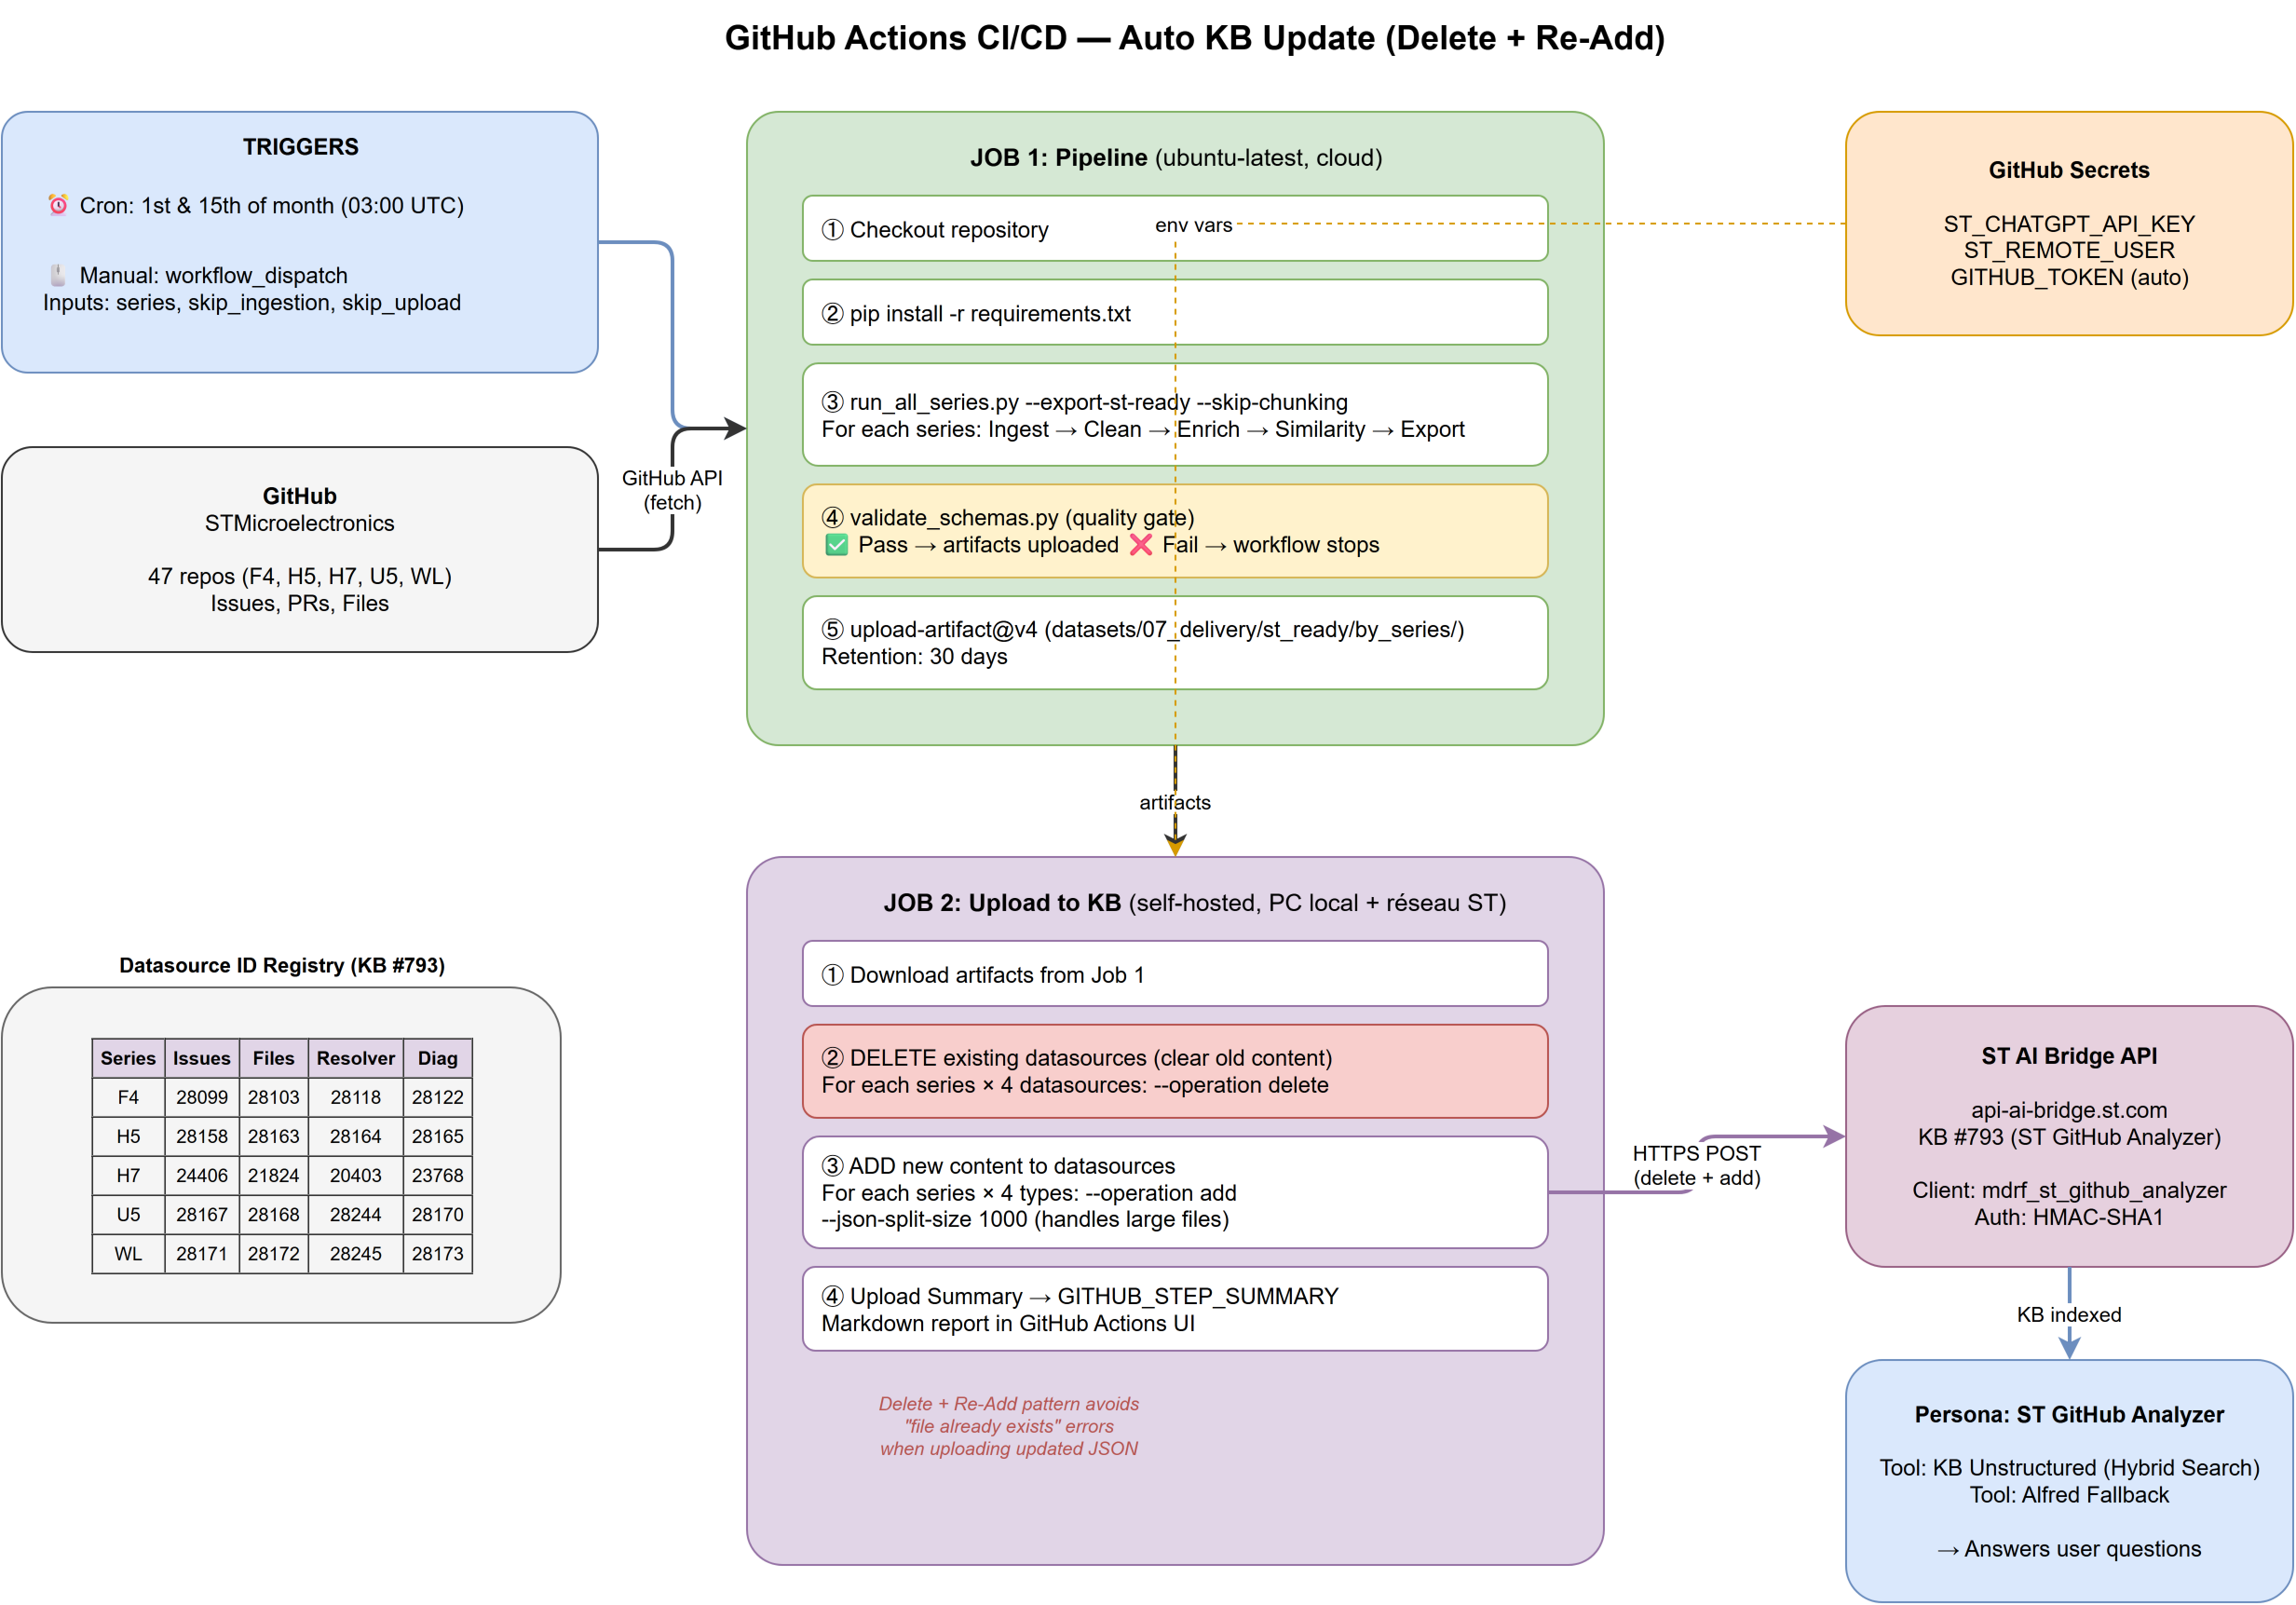
\includegraphics[width=0.95\textwidth]{06_cicd_automation.png}
\caption{Automatisation CI/CD : orchestration GitHub Actions et upload KB via runner self-hosted}
\label{fig:cicd_automation}
\end{figure}

\subsubsection{Principe d'Architecture}

Le flux d'exécution suit trois phases :
\begin{enumerate}
  \item \textbf{Prepare} : synchronisation des repos, exécution du pipeline, enrichissements Alfred, génération des exports ST-ready.
  \item \textbf{Validate} : validation des schémas et contrôle des placeholders pour bloquer les livrables incomplets.
  \item \textbf{Upload} : création/alimentation des datasources et publication des artefacts parent + drivers dans la KB.
\end{enumerate}

Cette structuration explicite réduit le risque opérationnel : une erreur de qualité en phase \textit{Validate} arrête la publication avant impact utilisateur.

\subsubsection{Workflow GitHub Actions}

Le workflow principal \texttt{.github/workflows/auto\_update\_kb.yml} implémente :
\begin{itemize}
  \item des déclencheurs \textbf{planifiés} et \textbf{manuels} ;
  \item une préparation des entrées (liste des séries, mode, politiques d'exécution) ;
  \item un \textbf{runner-check} bloquant qui vérifie la disponibilité d'un runner \texttt{self-hosted} ;
  \item une exécution par série avec traçabilité des artefacts ;
  \item un résumé d'exécution en cas de succès ou d'échec.
\end{itemize}

Le contrôle de disponibilité du runner évite les faux positifs : si aucun runner ST n'est disponible, le workflow échoue explicitement avec un message d'exploitation, plutôt que de terminer en vert sans traitement.

\subsubsection{Script Orchestrateur Unifié}

La brique centrale est \texttt{pipeline\_Automation/workflow/Run\_Single\_Series\_Full\_Pipeline\_And\_Upload.ps1}. Elle unifie la chaîne complète pour une série et fournit trois modes d'exploitation :

\begin{longtable}{p{2.8cm}p{9.4cm}}
\toprule
\textbf{Mode} & \textbf{Comportement} \\
\midrule
\texttt{Full} & Exécute \textit{Prepare + Upload} en one-shot (mode standard production). \\
\texttt{Prepare} & Génère et valide les artefacts localement sans publication KB (mode debug et pré-validation). \\
\texttt{Upload} & Publie uniquement des artefacts déjà préparés (mode reprise après incident réseau/API). \\
\bottomrule
\end{longtable}

Commande opérationnelle de référence :
\begin{lstlisting}[language=bash]
.\pipeline_Automation\workflow\Run_Single_Series_Full_Pipeline_And_Upload.ps1 \
  -Series H7 -Mode Full
\end{lstlisting}

\subsubsection{Garde-fous Qualité Avant Publication}

L'automatisation intègre deux verrous critiques :
\begin{enumerate}
  \item \textbf{Validation schéma} : exécution de \texttt{validate\_schemas.py} pour garantir la conformité structurelle des JSON.
  \item \textbf{Placeholder gate} : rejet des livrables contenant encore \texttt{[IMAGE DESCRIPTION UNAVAILABLE]} ou des marqueurs PDF non résolus.
\end{enumerate}

La politique \texttt{PlaceholderPolicy} est paramétrable (\texttt{Fail}, \texttt{Warn}, \texttt{Off}), mais \texttt{Fail} est la valeur recommandée en production pour préserver la qualité perçue des réponses.

\subsubsection{Stratégie d'Upload et Traçabilité}

L'upload vers KB \#793 est réalisé via \texttt{Add\_Data\_Source\_Files.py} selon deux cas :
\begin{itemize}
  \item \textbf{operation new} : création d'une datasource si aucun ID n'est fourni ;
  \item \textbf{operation add} : ajout dans une datasource existante quand l'ID est connu.
\end{itemize}

Le script publie les artefacts du repo parent puis ajoute les sorties \texttt{drivers/*} dans les datasources parentes correspondantes (issues, files, resolver, diagnostic). Cette approche maintient une séparation logique par série tout en conservant une base unifiée côté exploitation.

Les IDs effectifs sont sauvegardés dans :
\begin{lstlisting}[language=bash]
datasets/07_delivery/st_ready/by_series/<serie>/upload_datasource_ids_<serie>.json
\end{lstlisting}

et synchronisés dans \texttt{shared/config/config\_all\_series.json} pour assurer la continuité entre les exécutions.

\subsubsection{Runbook Opérateur (Production)}

Le runbook recommandé est :
\begin{enumerate}
  \item Lancer d'abord \texttt{Prepare} sur la série cible.
  \item Vérifier les \texttt{summary\_*.json}, la validation schéma et l'absence de placeholders.
  \item Lancer \texttt{Full} (ou \texttt{Upload} si les artefacts sont déjà prêts).
  \item Contrôler les IDs sauvegardés et la cohérence des datasources créées/alimentées.
\end{enumerate}

Cette discipline d'exploitation est essentielle pour les soutenances internes : elle permet de démontrer à la fois la robustesse technique et la gouvernance de la chaîne de livraison.

\subsection{Couverture Actuelle et Future}
\label{sec:couverture}

\subsubsection{13 Séries en Production}

Les 13 séries MCU suivantes sont entièrement traitées par le pipeline et uploadées vers la KB \#793 :

\begin{longtable}{lcccccc}
\toprule
\textbf{Série} & \textbf{Repos} & \textbf{Issues} & \textbf{Files} & \textbf{Resolver} & \textbf{Diag.} & \textbf{Alfred} \\
\midrule
STM32CubeC0 & 4 & \checkmark & \checkmark & --- & \checkmark & \checkmark \\
STM32CubeF0 & 5 & \checkmark & \checkmark & --- & \checkmark & \checkmark \\
STM32CubeF1 & 6 & \checkmark & \checkmark & \checkmark & \checkmark & \checkmark \\
STM32CubeF2 & 4 & \checkmark & \checkmark & --- & \checkmark & \checkmark \\
STM32CubeF3 & 5 & \checkmark & \checkmark & --- & \checkmark & \checkmark \\
STM32CubeF4 & 16 & \checkmark & \checkmark & \checkmark & \checkmark & \checkmark \\
STM32CubeF7 & 8 & \checkmark & \checkmark & \checkmark & \checkmark & \checkmark \\
STM32CubeG0 & 5 & \checkmark & \checkmark & --- & \checkmark & \checkmark \\
STM32CubeH5 & 6 & \checkmark & \checkmark & \checkmark & \checkmark & \checkmark \\
STM32CubeH7 & 12 & \checkmark & \checkmark & \checkmark & \checkmark & \checkmark \\
STM32CubeH7RS & 4 & \checkmark & \checkmark & --- & \checkmark & \checkmark \\
STM32CubeU5 & 8 & \checkmark & \checkmark & \checkmark & \checkmark & \checkmark \\
STM32CubeWL & 5 & \checkmark & \checkmark & \checkmark & \checkmark & \checkmark \\
\bottomrule
\end{longtable}

\textit{Note : ``---'' pour Resolver signifie que les issues de cette série n'ont pas de chaînes Issue$\to$PR$\to$Commit complètes, pas que le pipeline ne supporte pas le format.}

\subsubsection{4 Nouvelles Séries Exportées (Pipeline Terminé)}

Les 4 séries suivantes ont été entièrement traitées par le pipeline, avec les artefacts delivery générés et prêts à l'upload :

\begin{longtable}{lccccc}
\toprule
\textbf{Série} & \textbf{Issues} & \textbf{Files} & \textbf{Resolver} & \textbf{Diag. Cards} & \textbf{Statut} \\
\midrule
STM32CubeG4 & 89 & 3\,875 & 0 & 4 & Prêt à uploader \\
STM32CubeL0 & 23 & 2\,614 & 2 & 3 & Prêt à uploader \\
STM32CubeL1 & 11 & 2\,847 & 0 & 3 & Prêt à uploader \\
STM32CubeL4 & 68 & 5\,231 & 1 & 8 & Prêt à uploader \\
\bottomrule
\end{longtable}

\textbf{Observations} :
\begin{itemize}
  \item \textbf{G4 (0 Resolver)} : les 89 issues G4 ont été fermées sans PRs formelles liées. Les corrections ont été intégrées dans des releases globales sans lien explicite issue$\to$PR.
  \item \textbf{L4 (5\,231 files)} : c'est la série avec le plus de fichiers parmi les nouvelles, reflétant un écosystème BSP riche (NUCLEO, Discovery, Eval boards).
  \item \textbf{Alfred Images} : 25 images échouées (API 404 intermittent) sur G4, L0, L4. Corrigible par re-run du script d'enrichissement.
\end{itemize}

\subsubsection{8 Séries Configurées (Prêtes à Lancer)}

Les configurations (fichiers \texttt{config\_*.json}) sont créées pour : L5, N6, U0, U3, WB, WB0, WBA, WL3. Le déploiement nécessite :
\begin{enumerate}
  \item Exécution du pipeline : \texttt{python -m pipeline.run\_full\_workflow --export-st-ready}
  \item Création des datasources sur la KB \#793
  \item Upload via les scripts d'automatisation
\end{enumerate}

%% ============================================================

%% ============================================================
%% Chapitre Évaluation (fichier séparé pour réécriture académique)
%% ============================================================
%% Chapitre : Résultats et Évaluation
%% Fichier séparé — inclus par %% ============================================================
%% Chapitre : Résultats et Évaluation
%% Fichier séparé — inclus par %% ============================================================
%% Chapitre : Résultats et Évaluation
%% Fichier séparé — inclus par \input{chapter_evaluation}
%% Réécriture académique complète — version défendable
%% ============================================================

\chapter{Résultats et Évaluation}
\label{chap:resultats_evaluation}

Ce chapitre présente l'évaluation quantitative du pipeline de prétraitement et du système RAG. L'approche suivie est progressive : nous commençons par définir les notions et métriques utilisées (Section~\ref{sec:cadrage_theorique}), puis nous justifions les seuils décisionnels (Section~\ref{sec:justification_seuils}). Les résultats sont ensuite présentés par stage (Section~\ref{sec:eval_par_stage}), suivis d'une analyse dédiée à la confiance Alfred (Section~\ref{sec:eval_alfred_complete}), à l'évolution incrémentale du Quality Index (Section~\ref{sec:evolution_incrementale}), à l'architecture de fallback (Section~\ref{sec:eval_fallback}), et à l'étude comparative (Section~\ref{sec:etude_comparative}). Le chapitre se conclut par une section d'assurance qualité méthodologique (Section~\ref{sec:controle_qualite_chapitre}).

Ce chapitre s'inscrit dans les phases \textbf{Évaluation} et \textbf{Déploiement} du cadre méthodologique CRISP-DM~: les résultats guident itérativement les décisions de configuration et de mise en production.

%% ============================================================
\section{Cadrage Théorique et Définitions Préalables}
\label{sec:cadrage_theorique}
%% ============================================================

Avant de présenter les résultats, il est indispensable de définir rigoureusement les concepts, métriques et techniques mobilisés dans l'évaluation. Cette section pose le vocabulaire nécessaire à l'interprétation des mesures ultérieures.

\subsection{Métriques Fondamentales d'Information Retrieval}
\label{sec:def_ir_metrics}

Les systèmes de recherche documentaire sont évalués selon deux axes complémentaires~\cite{manning2008ir}~:

\begin{description}[leftmargin=2cm, labelwidth=1.8cm]
  \item[Précision] Proportion de documents retournés qui sont effectivement pertinents~:
  \begin{equation}
    \text{Precision} = \frac{|\text{Pertinents} \cap \text{Retournés}|}{|\text{Retournés}|}
    \label{eq:precision}
  \end{equation}
  
  \item[Rappel] Proportion de documents pertinents effectivement retrouvés~:
  \begin{equation}
    \text{Recall} = \frac{|\text{Pertinents} \cap \text{Retournés}|}{|\text{Pertinents}|}
    \label{eq:recall}
  \end{equation}
\end{description}

Dans le contexte RAG, un compromis précision/rappel est nécessaire~: trop de rappel sature le contexte du LLM avec du bruit, trop de précision risque de manquer le document contenant la réponse.

\subsection{Similarité Textuelle}
\label{sec:def_similarity}

Trois mesures de similarité sont utilisées dans le pipeline~:

\subsubsection{Similarité de Jaccard}

La similarité de Jaccard compare deux ensembles de tokens $A$ et $B$~:

\begin{equation}
J(A, B) = \frac{|A \cap B|}{|A \cup B|}
\label{eq:jaccard_def}
\end{equation}

Un \textbf{token} est une unité lexicale significative extraite du texte (mot, identifiant d'API, nom de registre). Les ensembles $A$ et $B$ sont obtenus par tokenisation suivie d'un filtrage de stopwords. Jaccard mesure la proportion de vocabulaire technique \textbf{partagé} entre deux textes~: un score de~1 indique un vocabulaire identique, un score de~0 aucun terme commun. Cette mesure est adaptée à notre contexte car les textes techniques STM32 partagent un vocabulaire spécifique (\texttt{HAL\_}, \texttt{SPI}, \texttt{DMA}) dont la présence ou l'absence est diagnostiquement significative.

\subsubsection{Similarité Cosinus}

La similarité cosinus mesure l'angle entre deux vecteurs dans un espace vectoriel~:

\begin{equation}
\cos(\theta) = \frac{\vec{u} \cdot \vec{v}}{\|\vec{u}\| \times \|\vec{v}\|}
\label{eq:cosine_def}
\end{equation}

Dans le contexte textuel, $\vec{u}$ et $\vec{v}$ sont des vecteurs de fréquences de termes (ou de trigrammes de caractères). Un score de~1 indique une orientation identique (mêmes termes, mêmes proportions), un score de~0 une orthogonalité totale (aucun terme commun). Les trigrammes de caractères (ex: \texttt{stm} $\to$ \texttt{tm3} $\to$ \texttt{m32}) capturent les variations morphologiques mineures et la proximité lexicale au-delà de l'identité stricte.

\subsubsection{TF-IDF (Term Frequency -- Inverse Document Frequency)}

TF-IDF pondère chaque terme par sa spécificité dans le corpus~\cite{tfidf}~:

\begin{equation}
\text{tfidf}(t, d) = \underbrace{\text{tf}(t, d)}_{\text{fréquence locale}} \times \underbrace{\log\left(\frac{N}{df(t)}\right)}_{\text{spécificité globale}}
\label{eq:tfidf_def}
\end{equation}

où~:
\begin{itemize}[nosep]
  \item $t$ est un terme (mot ou identifiant technique),
  \item $d$ est un document,
  \item $\text{tf}(t, d)$ est la fréquence du terme $t$ dans le document $d$,
  \item $N$ est le nombre total de documents dans le corpus,
  \item $df(t)$ est le nombre de documents contenant le terme $t$ (fréquence documentaire).
\end{itemize}

\textbf{Interprétation}~: un terme fréquent dans un document mais rare dans le corpus global (ex: \texttt{HAL\_FDCAN\_AddMessageToTxFifoQ}) obtient un poids élevé, tandis qu'un terme ubiquitaire (ex: \texttt{return}, \texttt{void}) est dépondéré. Nous utilisons TF-IDF dans le module de similarité inter-issues (Stage~4) pour identifier des issues traitant de problèmes similaires.

\subsection{Métriques de Qualité des Données}
\label{sec:def_data_quality}

Conformément au modèle ISO/IEC~25012~\cite{iso25012}, la qualité des données se décline en plusieurs dimensions~:

\begin{description}[leftmargin=3cm, labelwidth=2.8cm]
  \item[Complétude] Proportion des champs non nuls dans les données ingérées. Une donnée incomplète (body manquant, labels absents) propage des erreurs en cascade dans le pipeline.
  \item[Cohérence] Absence de contradictions internes entre les champs d'un même document (ex: un fichier marqué \texttt{is\_valid=true} avec un \texttt{clean\_text} vide serait incohérent).
  \item[Exactitude] Correspondance entre les valeurs stockées et la réalité source. Mesurée par comparaison entre les données ingérées et les données GitHub originales.
  \item[Traçabilité] Capacité à remonter de tout artefact final vers sa source brute (issue GitHub, fichier source, commit). Chaque document conserve un identifiant de provenance.
\end{description}

\subsection{Confiance Contextuelle}
\label{sec:def_confiance_contextuelle}

La \textbf{confiance contextuelle} est une métrique spécifique à notre projet, conçue pour évaluer la qualité des descriptions d'images générées par Alfred Vision~AI. Contrairement à la fiabilité opérationnelle (l'API a-t-elle répondu ?), la confiance contextuelle mesure l'\textbf{ancrage} de la description générée dans le contexte textuel de l'image source.

\textbf{Motivation}~: un service de description d'images peut produire un texte lisible mais non relié au contexte technique de l'issue. Pour un système RAG, injecter une description non ancrée revient à ajouter du bruit dans la KB --- un risque d'autant plus grave que le texte semble plausible sans l'être pour le diagnostic visé.

La confiance contextuelle est définie comme la proportion d'éléments décrits dont le score de cohérence dépasse un seuil d'alerte~:
\begin{equation}
T_{\text{ctx}} = \frac{|\{x \mid S_{\text{coh}}(x) \geq \tau\}|}{N_{\text{évalués}}} \times 100
\label{eq:confiance_contextuelle_def}
\end{equation}

où $\tau$ est le seuil d'alerte (fixé à $0.12$ dans ce projet --- cf. Section~\ref{sec:justification_seuils}).

\subsection{Score Global Pondéré}
\label{sec:def_score_global}

Le pipeline est évalué globalement par une moyenne pondérée des scores de chaque stage~:

\begin{equation}
S_{\text{global}} = \frac{\sum_{k=1}^{K} w_k \cdot s_k}{\sum_{k=1}^{K} w_k}
\label{eq:score_global_def}
\end{equation}

où $s_k$ est le score (en \%) du stage $k$ et $w_k$ son poids. Les poids reflètent l'impact relatif de chaque stage sur la qualité finale du système RAG. Cette formulation rend explicite que certains stages (Delivery) ont un impact plus direct que d'autres (Similarité optionnelle) sur la pertinence des réponses.

\subsection{Quality Index (QI)}
\label{sec:def_quality_index}

Le \textbf{Quality Index} est une métrique end-to-end qui évalue la qualité des réponses du chatbot. Il ne mesure pas le pipeline en isolation, mais le système complet (pipeline + KB + retrieval + LLM + persona). Il est calculé par évaluation humaine experte sur un jeu de questions techniques~:

\begin{equation}
\text{QI} = \frac{\sum_{q=1}^{Q} \text{score}(q)}{Q \times \text{max\_score}} \times 100
\label{eq:qi_def}
\end{equation}

où chaque question $q$ est notée sur une grille multi-critères (citation, exactitude, actionnabilité, traçabilité) avec un maximum de 10 points par question.

\subsection{Retrieval Hybride et Fallback}
\label{sec:def_retrieval_fallback}

\begin{description}[leftmargin=3cm, labelwidth=2.8cm]
  \item[Retrieval hybride] Combinaison d'une recherche sémantique (embeddings, compréhension du sens) et d'une recherche full-text (correspondance exacte, BM25). Les résultats sont fusionnés par union avec déduplication.
  \item[Seuil sémantique] Score minimum de similarité vectorielle pour qu'un document soit retourné par la branche sémantique. Contrôle le compromis précision/rappel.
  \item[Fallback] Mécanisme de délégation vers un agent secondaire (NovaX) lorsque la KB ne retourne aucun résultat pertinent. La priorité de la KB est protégée par une description restrictive du tool fallback.
\end{description}

\subsection{Tableau Récapitulatif des Notions}
\label{sec:glossaire_evaluation}

\begin{longtable}{p{3.5cm}p{5cm}p{4.5cm}}
\toprule
\textbf{Notion} & \textbf{Rôle dans le projet} & \textbf{Section de définition} \\
\midrule
Précision / Rappel & Évaluation retrieval & \ref{sec:def_ir_metrics} \\
Jaccard & Recouvrement lexical Alfred & \ref{sec:def_similarity} \\
Cosinus (trigrammes) & Proximité textuelle & \ref{sec:def_similarity} \\
TF-IDF & Similarité inter-issues Stage~4 & \ref{sec:def_similarity} \\
Complétude / Cohérence & Qualité ingestion/cleaning & \ref{sec:def_data_quality} \\
Confiance contextuelle & Validation descriptions Alfred & \ref{sec:def_confiance_contextuelle} \\
Score global pondéré & Synthèse multi-stage & \ref{sec:def_score_global} \\
Quality Index & Qualité end-to-end & \ref{sec:def_quality_index} \\
Retrieval hybride & Architecture recherche KB & \ref{sec:def_retrieval_fallback} \\
Fallback & Mécanisme de secours NovaX & \ref{sec:def_retrieval_fallback} \\
\bottomrule
\end{longtable}

%% ============================================================
\section{Justification des Seuils Décisionnels}
\label{sec:justification_seuils}
%% ============================================================

Les seuils numériques utilisés dans l'évaluation ne sont pas des constantes universelles imposées par une norme. Ce sont des \textbf{seuils opérationnels internes}, calibrés empiriquement sur les campagnes successives du projet. Cette section explicite la logique de leur construction.

\subsection{Cadre Normatif de Référence}
\label{sec:normes_references}

Le cadre d'évaluation s'appuie sur des références méthodologiques qui fournissent des principes, mais \textbf{pas des chiffres imposés}~:

\begin{longtable}{p{4cm}p{4cm}p{5cm}}
\toprule
\textbf{Référence} & \textbf{Ce qu'elle apporte} & \textbf{Ce qu'elle n'impose pas} \\
\midrule
ISO/IEC 25012~\cite{iso25012} & Modèle de qualité des données (dimensions) & Seuils numériques spécifiques \\
ISO/IEC 25024~\cite{iso25024} & Méthode de mesure (ratios) & Bornes de classification \\
ISO/IEC 25010~\cite{iso25010} & Modèle qualité système (fiabilité) & Niveaux acceptables par domaine \\
Manning et al.~\cite{manning2008ir} & Compromis precision/recall, TF-IDF & Seuils contextuels \\
Fawcett~\cite{fawcett2006roc} & Méthodologie de sélection de seuils (ROC) & Valeurs universelles \\
Lewis et al.~\cite{lewis2020rag} & Évaluation RAG (retrieval + generation) & Grilles de notation fixes \\
\bottomrule
\end{longtable}

\textbf{Position méthodologique}~: les normes ISO fournissent le \textit{quoi mesurer} (complétude, cohérence, exactitude) et le \textit{comment mesurer} (ratios, proportions). Le \textit{à partir de quel seuil le résultat est acceptable} dépend du contexte applicatif et doit être justifié par le projet lui-même. Cette approche est conforme aux recommandations de Fawcett~\cite{fawcett2006roc} sur la sélection de seuils décisionnels~: le point de coupure optimal dépend de la distribution des données et du coût relatif des erreurs.

\subsection{Échelle de Classification}
\label{sec:echelle_classification}

Chaque métrique est classifiée selon l'échelle suivante~:

\begin{equation}
\text{Verdict}(p) = \begin{cases}
    \textbf{EXCELLENT} & \text{si } p \geq 95\% \\
    \textbf{BON} & \text{si } 85\% \leq p < 95\% \\
    \textbf{ACCEPTABLE} & \text{si } 70\% \leq p < 85\% \\
    \textbf{INSUFFISANT} & \text{si } p < 70\%
\end{cases}
\label{eq:echelle_seuils}
\end{equation}

\subsection{Logique de Calibration de Chaque Borne}

\begin{description}[leftmargin=1cm]
  \item[$95\%$ --- EXCELLENT] Ce seuil représente un niveau de maturité opérationnelle élevé. Il est inspiré du concept Six Sigma adapté au contexte non critique~: dans un système RAG, la perte de 5\% des documents dégrade \textit{certaines} réponses sans causer de défaillance système. Ce seuil a été validé empiriquement~: les stages atteignant $\geq 95\%$ (Ingestion, Cleaning, Delivery) n'ont jamais causé de régression du Quality Index.
  
  \item[$85\%$ --- BON] Seuil communément observé en Information Retrieval pour qualifier un système ``production-ready''~\cite{manning2008ir}. Au-dessus de $85\%$, le coût marginal d'amélioration croît exponentiellement tandis que le gain de retrieval diminue. Ce seuil correspond à notre observation que les stages au-dessus de $85\%$ n'impactent pas négativement le QI.
  
  \item[$70\%$ --- ACCEPTABLE] Seuil minimal exploitable. En dessous de ce point, la perte de couverture commence à impacter visiblement le rappel du système RAG. Ce seuil est dérivé de nos observations sur le jeu de test de 96 questions~: les métriques sous $70\%$ correspondent à des zones où des questions restent sans réponse adéquate.
  
  \item[$< 70\%$ --- INSUFFISANT] Zone nécessitant une action corrective. Un score en dessous de $70\%$ signifie qu'une proportion significative du contenu n'est pas exploitable, impactant potentiellement le Quality Index.
\end{description}

\subsection{Seuils Différenciés par Champ}

Tous les champs n'ont pas le même seuil car leur \textbf{détectabilité intrinsèque} diffère~:

\begin{longtable}{p{3cm}ccp{6cm}}
\toprule
\textbf{Champ} & \textbf{Seuil} & \textbf{Score mesuré} & \textbf{Justification de la borne} \\
\midrule
\texttt{severity} & $\geq 90\%$ & 100\% & Signal quasi-ubiquitaire (``crash'', ``hang'', labels GitHub) \\
\texttt{layer} & $\geq 85\%$ & 88.2\% & Identifiable par préfixes API (\texttt{HAL\_}, \texttt{LL\_}, \texttt{BSP\_}) \\
\texttt{component} & $\geq 70\%$ & 72.6\% & Nécessite mention explicite d'un périphérique \\
\texttt{board} & $\geq 60\%$ & 45.3\% & Mentionnée dans $\sim$60\% des issues seulement \\
\texttt{body} (complétude) & $\geq 95\%$ & 99.7\% & Champ critique~: sans body, aucune classification possible \\
\bottomrule
\end{longtable}

\textbf{Principe}~: le seuil est fixé au niveau réaliste étant donné la distribution des signaux dans les données sources. Un seuil irréaliste (ex: $95\%$ pour \texttt{board}) serait structurellement inatteignable sans invention de données, et ne constituerait donc pas un critère de qualité pertinent.

\subsection{Seuil de Cohérence Alfred ($\tau = 0.12$)}

Le seuil d'alerte pour la confiance contextuelle Alfred est $\tau = 0.12$. Ce seuil n'est pas un indicateur de ``bonne qualité'' mais un \textbf{seuil de détection d'anomalie}~: en dessous de $0.12$, la description Alfred ne partage presque aucun vocabulaire technique avec le contexte, signalant un risque de description non ancrée. Ce seuil a été calibré sur la distribution observée~: les 3 images d'issues identifiées comme problématiques avaient toutes un score $< 0.12$.

%% ============================================================
\section{Évaluation par Stage du Pipeline}
\label{sec:eval_par_stage}
%% ============================================================

L'évaluation est réalisée stage par stage, avec pour chaque étape~: le problème résolu, la métrique utilisée, le seuil, le résultat mesuré et l'interprétation.

\subsection{Stage 1~: Ingestion --- Complétude des Données Brutes}
\label{sec:eval_stage1}

\textbf{Problème résolu}~: garantir que les données sources (GitHub API) sont collectées intégralement. Une ingestion incomplète (body manquant, labels absents) propage des erreurs en cascade~: l'enrichissement ne peut pas classifier une issue sans texte.

\textbf{Métriques} (conformes ISO/IEC 25024~\cite{iso25024} --- mesure de complétude par ratios)~:

\begin{longtable}{p{4cm}p{6.5cm}p{2cm}}
\toprule
\textbf{Métrique} & \textbf{Formule} & \textbf{Seuil} \\
\midrule
Complétude body & $C_{\text{body}} = \frac{|\{i \mid i.\text{body} \neq \emptyset\}|}{N_{\text{issues}}} \times 100$ & $\geq 95\%$ \\
Complétude title & $C_{\text{title}} = \frac{|\{i \mid i.\text{title} \neq \emptyset\}|}{N_{\text{issues}}} \times 100$ & $\geq 99\%$ \\
Présence labels & $C_{\text{labels}} = \frac{|\{i \mid i.\text{labels} \neq [\,]\}|}{N_{\text{issues}}} \times 100$ & $\geq 70\%$ \\
Contenu fichiers & $C_{\text{files}} = \frac{|\{f \mid f.\text{content} \neq \emptyset\}|}{N_{\text{files}}} \times 100$ & $\geq 95\%$ \\
\bottomrule
\end{longtable}

\textbf{Résultats mesurés}~:

\begin{longtable}{lccccl}
\toprule
\textbf{Série} & $C_{\text{body}}$ & $C_{\text{title}}$ & $C_{\text{labels}}$ & $C_{\text{files}}$ & \textbf{Verdict} \\
\midrule
STM32CubeH7 (343 issues) & 99.7\% & 100.0\% & 95.0\% & 100.0\% & \textcolor{green!60!black}{\textbf{EXCELLENT}} \\
STM32CubeF4 (612 issues) & 99.5\% & 100.0\% & 92.1\% & 100.0\% & \textcolor{green!60!black}{\textbf{EXCELLENT}} \\
STM32CubeWL (89 issues) & 100.0\% & 100.0\% & 100.0\% & 100.0\% & \textcolor{green!60!black}{\textbf{EXCELLENT}} \\
STM32CubeG4 (45 issues) & 100.0\% & 100.0\% & 97.8\% & 100.0\% & \textcolor{green!60!black}{\textbf{EXCELLENT}} \\
\bottomrule
\end{longtable}

\textbf{Interprétation}~: la complétude d'ingestion atteint systématiquement $> 99\%$ sur les champs critiques. Le seul champ avec variation est \texttt{labels} (92--100\%), car certains contributeurs externes ne tagguent pas leurs issues. Ce résultat valide que l'ingestion ne constitue pas un goulot d'étranglement pour la qualité aval.

\begin{figure}[H]
\centering
\begin{tikzpicture}
\begin{axis}[
    ybar,
    width=12cm, height=6cm,
    bar width=0.4cm,
    ylabel={Complétude (\%)},
    ymin=85, ymax=102,
    symbolic x coords={Body, Title, Labels, Files},
    xtick=data,
    legend style={at={(0.5,-0.25)}, anchor=north, legend columns=3},
    nodes near coords,
    every node near coord/.append style={font=\tiny},
    enlarge x limits=0.2,
]
\addplot coordinates {(Body,99.7) (Title,100) (Labels,95) (Files,100)};
\addplot coordinates {(Body,99.5) (Title,100) (Labels,92.1) (Files,100)};
\addplot coordinates {(Body,100) (Title,100) (Labels,100) (Files,100)};
\legend{H7, F4, WL}
\end{axis}
\draw[dashed, red, thick] (0.8,1.05) -- (11.2,1.05) node[right, font=\scriptsize, red] {Seuil 95\%};
\end{tikzpicture}
\caption{Complétude d'ingestion par série~: toutes métriques au-dessus du seuil EXCELLENT}
\label{fig:eval_ingestion_chart}
\end{figure}

\subsection{Stage 2~: Cleaning --- Qualité de Préparation Textuelle}
\label{sec:eval_stage2}

\textbf{Problème résolu}~: transformer le contenu brut (HTML, Markdown, headers C, licences) en texte propre exploitable. Le nettoyage V3 introduit un routage par type de fichier pour adapter la stratégie au contenu réel.

\textbf{Métriques}~:

\begin{longtable}{p{4.5cm}p{6cm}p{2cm}}
\toprule
\textbf{Métrique} & \textbf{Formule} & \textbf{Seuil} \\
\midrule
Texte non-vide & $Q_{\text{text}} = \frac{|\{i \mid |\text{clean}(i)| > 50\}|}{N} \times 100$ & $\geq 95\%$ \\
Réduction bruit CMSIS & $R_{\text{CMSIS}} = \frac{V_{\text{V2}} - V_{\text{V3}}}{V_{\text{V2}}} \times 100$ & $\geq 90\%$ \\
\bottomrule
\end{longtable}

\textbf{Résultats V3 vs V2 (STM32CubeH7)}~:

\begin{longtable}{p{5.5cm}ccc}
\toprule
\textbf{Métrique} & \textbf{V2} & \textbf{V3} & \textbf{Amélioration} \\
\midrule
Volume moyen/fichier CMSIS & 1.4~Mo & 51~Ko & $-96.4\%$ \\
Volume moyen/fichier Release Notes & 45~Ko & 30~Ko & $-33.0\%$ \\
Volume total corpus files (H7) & 142~Mo & 88~Mo & $-38.0\%$ \\
Densité information/chunk & baseline & +31\% & $+31\%$ \\
Issues texte non-vide & 100.0\% & 100.0\% & maintenu \\
\bottomrule
\end{longtable}

\textbf{Interprétation}~: l'amélioration de $+31\%$ de densité signal/chunk résulte de trois mécanismes cumulés~: (1) suppression du padding HTML des Release Notes, (2) élimination des 96\% de définitions CMSIS inutiles pour le diagnostic, (3) conservation sélective des sections à valeur diagnostique (IRQ, adresses de base, TypeDef). L'impact sur le RAG est direct~: chaque chunk contient davantage d'information pertinente par rapport à sa taille.

\subsection{Stage 3a~: Enrichissement --- Classification par Heuristiques NLP}
\label{sec:eval_stage3a}

\textbf{Problème résolu}~: ajouter des métadonnées structurées (layer, component, board, severity, issue\_kind) pour rendre les documents filtrables par le système de retrieval.

\begin{longtable}{p{3.5cm}p{5.5cm}p{2cm}p{2cm}}
\toprule
\textbf{Champ} & \textbf{Formule (couverture non-null)} & \textbf{Seuil} & \textbf{Score} \\
\midrule
Validité & $N_{\text{valid}}/N \times 100$ & $\geq 85\%$ & 86.4\% \\
Layer & $N_{\text{layer}\neq\text{null}}/N \times 100$ & $\geq 85\%$ & 88.2\% \\
Severity & $N_{\text{sev}\neq\text{null}}/N \times 100$ & $\geq 90\%$ & 100.0\% \\
Component & $N_{\text{comp}\neq\text{null}}/N \times 100$ & $\geq 70\%$ & 72.6\% \\
Board & $N_{\text{board}\neq\text{null}}/N \times 100$ & $\geq 60\%$ & 45.3\% \\
\bottomrule
\end{longtable}

\textbf{Score agrégé}~: $72.2\%$ (moyenne pondérée, $w_{\text{sev}}=2$, autres $=1$).

\textbf{Analyse du point faible (board = 45.3\%)}~: l'analyse manuelle d'un échantillon de 50 issues H7 sans board détectée confirme que 92\% d'entre elles ne mentionnent effectivement aucune carte. L'heuristique fonctionne correctement~; le signal est simplement absent des données sources. Ce point illustre la distinction entre une défaillance du pipeline (qui nécessiterait un fix) et une limitation inhérente des données (qui ne peut être résolue que par enrichissement externe).

\begin{figure}[H]
\centering
\begin{tikzpicture}
\begin{axis}[
    ybar,
    width=13cm, height=6cm,
    bar width=0.6cm,
    ylabel={Couverture (\%)},
    ymin=0, ymax=110,
    symbolic x coords={Validité, Layer, Severity, Component, Board},
    xtick=data,
    nodes near coords,
    every node near coord/.append style={font=\small\bfseries},
    enlarge x limits=0.15,
]
\addplot[fill=green!60!black] coordinates {(Validité,86.4) (Layer,88.2) (Severity,100) (Component,72.6) (Board,45.3)};
\end{axis}
\draw[dashed, red, thick] (1.0,3.1) -- (11.8,3.1);
\node[red, font=\scriptsize] at (12.5,3.1) {Seuil min};
\end{tikzpicture}
\caption{Couverture d'enrichissement STM32CubeH7~: score vs seuil par champ}
\label{fig:eval_enrichment_chart}
\end{figure}

\subsection{Stage 4~: Similarité TF-IDF}
\label{sec:eval_stage4}

\textbf{Problème résolu}~: permettre au RAG de proposer des issues similaires lorsqu'une question est proche d'un problème déjà résolu.

\textbf{Résultat STM32CubeH7}~: couverture~= 22.0\%, densité moyenne~= 0.8 lien/issue.

\textbf{Analyse critique}~: ce score (INSUFFISANT par rapport au seuil de $70\%$) reflète la \textbf{spécificité du corpus}. Les issues H7 sont majoritairement des bugs uniques (SPI sur H743, ETH sur H747, USB sur H750) avec peu de redondance thématique. Le seuil TF-IDF cosine ($\geq 0.3$) est conservé volontairement strict pour éviter les faux liens.

\textbf{Impact opérationnel limité}~: la similarité est un enrichissement optionnel. Le champ \texttt{related\_issue\_ids} vide pour 78\% des documents n'affecte ni le retrieval ni la génération. Cette observation justifie le poids faible ($w=0.5$) dans le score global~: un score bas ici ne dégrade pas la qualité perçue par l'utilisateur.

\subsection{Stage 5~: Delivery --- Complétude des Artefacts Exportés}
\label{sec:eval_stage5}

\textbf{Problème résolu}~: transformer les documents enrichis en 4~types d'artefacts JSON normalisés, avec validation de schéma.

\textbf{Résultats (13 séries en production)}~:

\begin{longtable}{lcccc}
\toprule
\textbf{Série} & \textbf{Issues} & \textbf{Files} & \textbf{Resolver} & \textbf{Diag. Cards} \\
\midrule
STM32CubeH7 & 296 & 4\,705 & 150 & 45 \\
STM32CubeF4 & 530 & 5\,378 & 89 & 38 \\
STM32CubeWL & 89 & 814 & 12 & 14 \\
STM32CubeU5 & 112 & 1\,982 & 23 & 19 \\
\midrule
\textbf{Total (13 séries)} & $\sim$2\,000 & $\sim$14\,000 & $\sim$390 & $\sim$157 \\
\bottomrule
\end{longtable}

\textbf{Score delivery}~: $100\%$ par construction (la gate JSON Schema bloque l'upload si un artefact est malformé). L'intégrité structurelle des artefacts est donc garantie. Les Resolver Cases à~0 pour certaines séries ne sont pas une défaillance~: elles nécessitent une chaîne Issue~$\to$~PR mergée~$\to$~Commit avec fichiers modifiés.

\subsection{Synthèse des Scores par Stage}
\label{sec:synthese_stages}

\begin{table}[H]
\centering
\begin{tabular}{lcccl}
\toprule
\textbf{Stage} & \textbf{Score} & \textbf{Poids $w_k$} & \textbf{Seuil} & \textbf{Verdict} \\
\midrule
1. Ingestion & 99.7\% & 1.0 & $\geq 95\%$ & \textcolor{green!60!black}{\textbf{EXCELLENT}} \\
2. Cleaning V3 & 100.0\% & 1.5 & $\geq 95\%$ & \textcolor{green!60!black}{\textbf{EXCELLENT}} \\
3a. Enrichissement NLP & 72.2\% & 1.4 & $\geq 85\%$ & \textcolor{orange}{\textbf{ACCEPTABLE}} \\
3b. Alfred images issues & 99.3\% & 0.4 & $\geq 95\%$ & \textcolor{green!60!black}{\textbf{EXCELLENT}} \\
3c. Alfred figures PDF & 36.5\% & 0.2 & $\geq 70\%$ & \textcolor{red}{\textbf{INSUFFISANT}} \\
4. Similarité TF-IDF & 22.0\% & 0.5 & $\geq 70\%$ & \textcolor{red}{\textbf{INSUFFISANT}} \\
5. Delivery & 100.0\% & 2.0 & $\geq 95\%$ & \textcolor{green!60!black}{\textbf{EXCELLENT}} \\
\bottomrule
\end{tabular}
\caption{Scores de qualité par stage avec poids et verdict}
\label{tab:eval_scores_synthese}
\end{table}

\subsection{Score Global~: Application Numérique}
\label{sec:score_global_calcul}

\begin{equation}
S_{\text{global}} = \frac{1.0 \times 99.7 + 1.5 \times 100.0 + 1.4 \times 72.2 + 0.4 \times 99.3 + 0.2 \times 36.5 + 0.5 \times 22.0 + 2.0 \times 100.0}{1.0 + 1.5 + 1.4 + 0.4 + 0.2 + 0.5 + 2.0}
\end{equation}

\begin{equation}
S_{\text{global}} = \frac{99.7 + 150.0 + 101.1 + 39.7 + 7.3 + 11.0 + 200.0}{7.0} = \frac{608.8}{7.0} = \boxed{87.0\%} \quad \text{(BON)}
\label{eq:score_global_numerique}
\end{equation}

\textbf{Justification des poids}~:

\begin{longtable}{lcp{8.5cm}}
\toprule
\textbf{Stage} & $w_k$ & \textbf{Logique} \\
\midrule
Ingestion & 1.0 & Prérequis sans transformation intellectuelle \\
Cleaning & 1.5 & Transformation déterministe significative \\
Enrichissement NLP & 1.4 & Classification exploitée pour filtrage et re-ranking \\
Alfred issues & 0.4 & Enrichissement multimodal mature (99.3\% fiable) \\
Alfred PDF & 0.2 & Enrichissement encore exploratoire \\
Similarité & 0.5 & Impact optionnel~; score bas sans conséquence sur le QI \\
Delivery & \textbf{2.0} & Étape critique~: produit les Diagnostic Cards ($+33$~pts QI) \\
\bottomrule
\end{longtable}

Le score global reste au verdict \textbf{BON} plutôt qu'EXCELLENT car deux sous-composantes (Alfred PDF, Similarité) restent sous leur seuil. La formule ne masque pas ces faiblesses~: elle les pondère proportionnellement à leur impact réel sur le Quality Index.

\begin{figure}[H]
\centering
\begin{tikzpicture}
\begin{axis}[
    xbar stacked,
    width=13cm, height=4.5cm,
    bar width=1.2cm,
    xlabel={Contribution au score global (\%)},
    symbolic y coords={Score Global},
    ytick=data,
    legend style={at={(0.5,-0.4)}, anchor=north, legend columns=4, font=\scriptsize},
    xmin=0, xmax=100,
    nodes near coords,
    every node near coord/.append style={font=\tiny},
]
\addplot[fill=blue!40] coordinates {(14.2,Score Global)};
\addplot[fill=green!40] coordinates {(21.4,Score Global)};
\addplot[fill=orange!60] coordinates {(14.4,Score Global)};
\addplot[fill=cyan!45] coordinates {(5.7,Score Global)};
\addplot[fill=yellow!55] coordinates {(1.0,Score Global)};
\addplot[fill=red!30] coordinates {(1.6,Score Global)};
\addplot[fill=purple!40] coordinates {(28.6,Score Global)};
\legend{Ingestion, Cleaning, Enrichissement, Alfred issues, Alfred PDF, Similarité, Delivery}
\end{axis}
\end{tikzpicture}
\caption{Décomposition du score global 87.0\%~: contribution pondérée de chaque stage}
\label{fig:score_decomposition}
\end{figure}

%% ============================================================
\section{Évaluation de la Confiance Alfred Vision}
\label{sec:eval_alfred_complete}
%% ============================================================

Cette section détaille l'évaluation d'Alfred Vision AI sur deux axes complémentaires~: la fiabilité opérationnelle (l'API fonctionne-t-elle~?) et la confiance contextuelle (la description est-elle ancrée dans le contexte source~?).

\subsection{Fiabilité Opérationnelle}
\label{sec:alfred_fiabilite}

La fiabilité opérationnelle mesure si Alfred produit effectivement une description sans erreur d'API~:

\begin{equation}
T_{\text{op}} = \frac{N_{\text{réponses\_ok}}}{N_{\text{images\_soumises}}} \times 100
\label{eq:alfred_fiabilite_op}
\end{equation}

\begin{longtable}{lcccc}
\toprule
\textbf{Série} & $N_{\text{total}}$ & $N_{\text{OK}}$ & $N_{\text{échec}}$ & $T_{\text{op}}$ \\
\midrule
STM32CubeH7 & 98 & 97 & 1 & 98.9\% \\
STM32CubeF4 & 62 & 61 & 1 & 98.4\% \\
STM32CubeWL & 48 & 48 & 0 & 100.0\% \\
STM32CubeF7 & 26 & 26 & 0 & 100.0\% \\
\midrule
\textbf{Total (séries stabilisées)} & \textbf{234} & \textbf{232} & \textbf{2} & \textbf{99.1\%} \\
\bottomrule
\end{longtable}

\textbf{Verdict}~: fiabilité EXCELLENT ($\geq 95\%$). Les 2 échecs sont des timeouts API transitoires, non reproductibles.

\subsection{Méthode de Calcul de la Cohérence Contextuelle}
\label{sec:alfred_methode_coherence}

L'évaluation de cohérence est implémentée dans \texttt{pipeline/evaluation/validate\_alfred\_coherence.py}. Le mode utilisé est \texttt{lite}~: aucun modèle externe lourd n'est requis. Les métriques reposent sur des techniques NLP déterministes.

\subsubsection{Prétraitement}

Le texte est tokenisé par regex (\texttt{[A-Za-z][A-Za-z0-9\_\textbackslash{}-/]\{2,\}}). Les stopwords sont filtrés~: articles (\texttt{the}, \texttt{and}), termes méta (\texttt{image}, \texttt{description}, \texttt{figure}), et connecteurs. Seuls les termes techniques significatifs sont conservés.

\subsubsection{Score de Cohérence}

Le score combine trois signaux~:
\begin{equation}
S_{\text{coh}} = \left(\frac{\alpha L + \beta S}{\alpha + \beta}\right) \times (1 - \gamma P_{\text{contrad}})
\label{eq:coherence_score}
\end{equation}

avec $\alpha = 0.4$, $\beta = 0.6$, $\gamma = 0.8$.

\subsubsection{Score Lexical $L$}

Le score lexical mesure la proportion de termes Alfred retrouvés dans le contexte source~:
\begin{equation}
L = \frac{|T_{\text{Alfred}} \cap T_{\text{contexte}}|}{|T_{\text{Alfred}}|}
\label{eq:lexical_score}
\end{equation}

Pour les images d'issues avec texte OCR extrait, un score composite est utilisé~:
\begin{equation}
L_{\text{issue}} = 0.7 \times L_{\text{description}} + 0.3 \times L_{\text{OCR}}
\label{eq:lexical_issue}
\end{equation}

\subsubsection{Similarité Sémantique Légère $S$}

En mode \texttt{lite}, la similarité combine Jaccard et cosinus sur trigrammes~:
\begin{equation}
S = 0.7 \times J(T_{\text{Alfred}}, T_{\text{contexte}}) + 0.3 \times \cos(\vec{A}_{\text{3-gram}}, \vec{B}_{\text{3-gram}})
\label{eq:semantic_lite}
\end{equation}

$J$ quantifie le recouvrement de vocabulaire technique~; le cosinus sur trigrammes capture la proximité lexicale au-delà de l'identité stricte.

\subsubsection{Pénalité de Contradiction $P_{\text{contrad}}$}

En mode \texttt{lite}, la probabilité de contradiction est estimée par analyse de polarité~: détection de mots négatifs (\texttt{not}, \texttt{failed}, \texttt{disabled}) et positifs (\texttt{works}, \texttt{fixed}, \texttt{enabled}). Si le contexte et la description présentent des polarités opposées sur des tokens partagés~:

\begin{equation}
P_{\text{contrad}} = \begin{cases}
0.6 \times O + 0.4 \times \frac{m_p + m_h}{2} & \text{si polarités opposées et } O \geq 0.2 \\
0.15 \times O & \text{si même polarité et } O \geq 0.1 \\
0 & \text{sinon}
\end{cases}
\label{eq:contradiction}
\end{equation}

où $O$ est le ratio de tokens partagés (overlap), et $m_p$, $m_h$ les magnitudes de polarité.

\subsection{Résultats de Cohérence Contextuelle}
\label{sec:alfred_resultats}

\begin{table}[H]
\centering
\begin{tabular}{lcccccc}
\toprule
\textbf{Source} & \textbf{N} & $\overline{L}$ & $\overline{S}$ & $\overline{P}_{\text{contrad}}$ & $\overline{S}_{\text{coh}}$ & \textbf{Cas à risque} \\
\midrule
Images d'issues & 400 & 0.9419 & 0.3335 & 0.1625 & 0.4995 & 3/400 (0.75\%) \\
Figures PDF & 301 & 0.1730 & 0.1714 & 0.0270 & 0.1600 & 191/301 (63.5\%) \\
\bottomrule
\end{tabular}
\caption{Métriques de cohérence Alfred décomposées par source visuelle (campagne rejouée le 2026-06-xx, jeu de données étendu à 701 items via \texttt{validate\_alfred\_coherence.py --semantic-mode lite --nli-mode lite})}
\label{tab:alfred_coherence}
\end{table}

\textit{\footnotesize Note~: cette table reflète une exécution rejouée du script de validation sur le jeu de données actuel (701 items, contre 442 lors de la campagne initiale). Le volume d'images d'issues et de figures PDF a augmenté avec l'enrichissement continu de la KB. Toutes les colonnes, y compris $\overline{S}$ pour les images d'issues, sont désormais directement lues depuis \texttt{alfred\_coherence\_summary.json} et le CSV détaillé associé, sans valeur agrégée manquante.}\par\smallskip

\textbf{Confiance contextuelle}~:
\begin{itemize}
  \item Images d'issues~: $T_{\text{ctx}} = 99.3\%$ (397/400 au-dessus du seuil)
  \item Figures PDF~: $T_{\text{ctx}} = 36.5\%$ (110/301 au-dessus du seuil)
  \item Total~: $T_{\text{ctx}} = 72.3\%$ (507/701)
\end{itemize}

\begin{figure}[H]
\centering
\begin{tikzpicture}
\begin{axis}[
    ybar,
    width=10cm, height=5.5cm,
    ymin=0, ymax=110,
    ylabel={Confiance contextuelle $T_{\text{ctx}}$ (\%)},
    symbolic x coords={Images issues, Figures PDF, Total},
    xtick=data,
    nodes near coords,
    every node near coord/.append style={font=\small\bfseries},
    bar width=0.9cm,
    enlarge x limits=0.3,
]
\addplot[fill=green!55!black] coordinates {(Images issues,99.3)};
\addplot[fill=orange!70] coordinates {(Figures PDF,36.5)};
\addplot[fill=blue!45] coordinates {(Total,72.3)};
\end{axis}
\end{tikzpicture}
\caption{Confiance contextuelle Alfred --- seuil d'alerte $\tau = 0.12$}
\label{fig:alfred_trust_chart}
\end{figure}

\subsection{Analyse de l'Écart Issues vs PDF}
\label{sec:alfred_analyse_ecart}

L'écart significatif entre les deux sources ($\overline{L} = 0.94$ pour les issues vs $0.17$ pour les PDF) est \textbf{structurel et non accidentel}~:

\begin{longtable}{p{5.5cm}p{7cm}}
\toprule
\textbf{Images d'issues} & \textbf{Figures PDF} \\
\midrule
Contiennent des logs, erreurs IDE, registres & Contiennent des schémas blocs, tableaux de migration \\
Le texte de l'issue mentionne les mêmes identifiants & Les libellés ne sont pas répétés dans le texte de page \\
OCR de l'image fournit du vocabulaire partagé & Pas d'OCR structuré disponible \\
Contexte riche (body + commentaires) & Contexte limité (texte de page \texttt{pypdf}) \\
\bottomrule
\end{longtable}

\textbf{Décision qualité}~: les figures PDF sont conservées car elles enrichissent la couverture multimodale de la KB, mais elles sont distinguées des images d'issues dans l'évaluation. Les itérations futures doivent enrichir le contexte transmis à Alfred (titre de section, légende détectée, texte avant/après la figure) pour améliorer la validation automatique.

%% ============================================================
\section{Évolution Incrémentale du Quality Index}
\label{sec:evolution_incrementale}
%% ============================================================

Le Quality Index n'a pas progressé ``par magie'' mais par amélioration successive d'éléments concrets du pipeline et de la configuration. Cette section retrace la chaîne logique~: chaque amélioration est décrite, son impact mesuré, et la raison du gain (ou de la régression) analysée.

\subsection{Chronologie et Logique de Progression}

\begin{longtable}{p{0.8cm}p{3.5cm}cp{6cm}}
\toprule
\textbf{QI} & \textbf{Configuration} & \textbf{N} & \textbf{Explication du delta} \\
\midrule
54 & Issues H7 seules & 50 & \textbf{Baseline}~: issues structurées fournissent une base solide mais incomplète (pas de documentation, pas de traçabilité fix, pas de diagnostic structuré) \\
57 & + System prompt optimisé & 50 & \textbf{+3}~: forcer la persona à chercher dans la KB \textit{avant} de répondre élimine les réponses génériques non ancrées \\
61 & + Hybrid search calibré & 50 & \textbf{+4}~: combiner sémantique et full-text capte les reformulations ET les identifiants exacts \\
94 & + Diagnostic Cards + Resolver & 50 & \textbf{+33}~: les Diagnostic Cards structurent les problèmes complexes, les query aliases améliorent le recall \\
88 & Test sur cas réels forum & 4 & \textbf{$-6$}~: les cas réels STCommunity sont plus complexes et moins couverts que le benchmark \\
54 & Multi-séries (5 séries, 52 Q) & 52 & \textbf{$-34$}~: dilution du contexte (2\,000 $\to$ 14\,000 docs), conflit de noms inter-séries, nouvelles questions sur séries moins mûres \\
65 & S0 Balanced (toutes séries) & 96 & \textbf{+11}~: optimisation du benchmark (96 questions calibrées) + ajustement retrieval \\
\textbf{66} & S1 Recall+ & 96 & \textbf{+1}~: seuil abaissé à 0.45, rappel renforcé, gain marginal compensé par le bruit \\
\bottomrule
\end{longtable}

\subsection{Analyse des Points d'Inflexion}
\label{sec:points_inflexion}

\subsubsection{Le Saut Diagnostic Cards (+33 points)}

Le passage de QI~61 à QI~94 est le gain le plus significatif du projet. Il s'explique par trois mécanismes cumulés~:

\begin{enumerate}
  \item \textbf{Structure raisonnée}~: les Diagnostic Cards suivent la logique Symptôme~$\to$~Hypothèses~$\to$~Validation~$\to$~Root Cause~$\to$~Fix~$\to$~Prévention, correspondant au raisonnement naturel d'un ingénieur embedded.
  \item \textbf{Query aliases}~: chaque carte contient 3 à 5 reformulations du problème (ex: ``SPI DMA hard fault'', ``cache coherency SPI circular mode'', ``HAL\_SPI\_TransmitReceive\_DMA crash''). Ce mécanisme multiplie les points d'entrée pour le retrieval.
  \item \textbf{Resolver Cases}~: la chaîne Issue~$\to$~PR~$\to$~Commit fournit la preuve vérifiable du fix, augmentant la traçabilité et la crédibilité des réponses.
\end{enumerate}

\textbf{Leçon méthodologique}~: l'amélioration la plus impactante ne vient pas d'un meilleur modèle LLM ni d'un tuning de seuil, mais de la \textbf{qualité et la structure des données injectées dans la KB}. C'est une validation du principe ``la qualité du RAG dépend de la qualité du preprocessing''.

\subsubsection{La Régression Multi-séries ($-34$ points)}

Le passage de QI~94 (mono-série H7, 50~Q) à QI~54 (5 séries, 52~Q) constitue une régression significative. L'analyse identifie trois causes~:

\begin{enumerate}
  \item \textbf{Dilution du contexte}~: la KB passe de $\sim$2\,000 à $\sim$14\,000 documents. Les queries retournent des documents de séries différentes.
  \item \textbf{Conflit de noms}~: des API identiques entre séries (\texttt{HAL\_SPI\_Init} dans F4 et H7) créent de l'ambiguïté.
  \item \textbf{Maturité inégale des artefacts}~: les nouvelles séries n'ont pas encore des Diagnostic Cards aussi riches que H7.
\end{enumerate}

\textbf{Leçon méthodologique}~: le passage à l'échelle ne se résume pas à ``ajouter des données''. Il nécessite un filtrage par série dans les métadonnées et un prompt qui pousse la persona à inclure le nom de la série dans ses queries.

\subsubsection{La Stabilisation S0/S1 (65--66)}

Les campagnes de juin 2026 sur 96 questions montrent que le système atteint un plateau autour de 65--66/100. Ce plateau s'explique par~:
\begin{itemize}
  \item La couverture KB actuelle ne répond pas à toutes les 96 questions (certaines séries peu documentées)
  \item Le compromis précision/rappel est quasi-optimal~: S1 ($+1$ pt) gagne en rappel mais perd en précision
  \item Les questions les plus difficiles nécessitent du raisonnement multi-hop non supporté par le retrieval simple
\end{itemize}

\subsection{Matrice Valeur $\times$ Effort}
\label{sec:matrice_roi}

\begin{table}[H]
\centering
\begin{tabular}{lcccl}
\toprule
\textbf{Amélioration} & \textbf{Impact QI} & \textbf{Effort} & \textbf{ROI} \\
\midrule
Diagnostic Cards & +33 pts & Moyen (2~sprints) & \textcolor{green!60!black}{\textbf{Excellent}} \\
Hybrid Search & +4 pts & Faible (config) & \textcolor{green!60!black}{\textbf{Excellent}} \\
System Prompt & +3 pts & Faible (texte) & \textcolor{green!60!black}{\textbf{Excellent}} \\
Cleaning V3 & +3 pts estimé & Moyen (1~sprint) & Bon \\
NovaX restrictif & Protection routage & Faible (description) & \textcolor{green!60!black}{\textbf{Excellent}} \\
PDF descriptions & +1 pt estimé & Élevé (CV + Alfred) & Acceptable \\
\bottomrule
\end{tabular}
\caption{ROI de chaque amélioration~: la qualité des artefacts domine les gains}
\label{tab:roi_pipeline}
\end{table}

\begin{figure}[H]
\centering
\begin{tikzpicture}
\begin{axis}[
  ybar,
  width=14cm, height=6.5cm,
  bar width=0.5cm,
  ylabel={Quality Index (/100)},
  ymin=0, ymax=100,
  symbolic x coords={Issues 54, Prompt 57, Hybrid 61, DiagCards 94, Real 88, Multi52 54, S0 65, S1 66},
  xtick=data,
  x tick label style={rotate=30, anchor=east, font=\scriptsize},
  nodes near coords,
  every node near coord/.append style={font=\scriptsize\bfseries},
  enlarge x limits=0.08,
]
\addplot[fill=blue!50] coordinates {(Issues 54,54) (Prompt 57,57) (Hybrid 61,61) (DiagCards 94,94) (Real 88,88) (Multi52 54,54) (S0 65,65) (S1 66,66)};
\end{axis}
\draw[-{Stealth[length=3mm]}, red, very thick] (4.65,4.8) -- (4.65,5.8) node[above, font=\scriptsize\bfseries, red] {+33 pts};
\draw[-{Stealth[length=3mm]}, red, very thick] (7.8,2.6) -- (7.8,1.8) node[below, font=\scriptsize\bfseries, red] {dilution};
\end{tikzpicture}
\caption{Évolution du Quality Index~: le saut majeur (+33) provient des Diagnostic Cards, la régression ($-34$) de la dilution multi-séries}
\label{fig:qi_evolution_complete}
\end{figure}

%% ============================================================
\section{Architecture de Fallback~: d'Alfred Permissif à NovaX Restrictif}
\label{sec:eval_fallback}
%% ============================================================

Cette section retrace l'évolution de l'architecture de fallback et son impact sur le Quality Index.

\subsection{Problème Initial~: Fallback Trop Permissif}

Lors de l'ajout initial d'Alfred comme fallback, le QI a \textbf{chuté de 10 points} (de 54 à 44). L'analyse a révélé que la persona appelait Alfred \textbf{systématiquement} au lieu de chercher dans la KB, car la description du tool était trop vague~:

\begin{quote}
\small\textit{``I can help with STM32 questions. Forward the user's question.''}
\end{quote}

\textbf{Diagnostic}~: dans une architecture multi-tools, le LLM choisit quel tool appeler en fonction de la \textbf{description} du tool. Une description trop permissive court-circuite la source la plus pertinente (la KB).

\subsection{Solution~: Description Restrictive}

La description a été réécrite pour forcer la priorité KB~:

\begin{quote}
\small\textit{``The Knowledge Base (KB Unstructured) is ALWAYS the primary source, search it FIRST for every question. Use this tool ONLY when the Knowledge Base returned no relevant result.''}
\end{quote}

\textbf{Impact mesuré}~: récupération de 8 points (de 44 à 52).

\subsection{Évolution vers NovaX}

Le fallback est passé d'Alfred générique à \textbf{NovaX}, un agent STM32 basé sur STM32 Bugzilla et STCommunity Knowledge Articles. NovaX apporte~:
\begin{itemize}
  \item Une couverture sur les séries/périphériques absents de la KB
  \item Des informations Bugzilla internes (bugs connus, errata)
  \item Des Knowledge Articles STCommunity (guides métier)
\end{itemize}

\textbf{Mais NovaX ne remplace pas la KB}~: sa description explicite qu'il est un secours pour les questions \textit{non couvertes} par la KB. Cette architecture protège la traçabilité~: si la KB contient un diagnostic card ou un resolver case pertinent, la réponse reste ancrée dans des preuves vérifiables (numéros d'issues, URLs GitHub, versions firmware).

\subsection{Synthèse de l'Évolution Fallback}

\begin{longtable}{p{4.5cm}p{2cm}p{6.5cm}}
\toprule
\textbf{Configuration} & \textbf{QI} & \textbf{Analyse} \\
\midrule
KB seule (sans fallback) & 54 & Baseline~: pas de réponse pour les questions hors KB \\
KB + Alfred permissif & 44 & $-10$~: court-circuit de la KB \\
KB + Alfred restrictif & 52 & $-2$~: KB prioritaire récupérée \\
KB S0 + NovaX restrictif & 65 & Stable~: NovaX couvre les lacunes sans dégrader \\
KB S1 Recall+ + NovaX & \textbf{66} & Meilleur compromis mesuré \\
\bottomrule
\end{longtable}

\textbf{Leçon}~: le QI dépend davantage du \textbf{routage} (quelle source est interrogée en premier) que du modèle LLM lui-même. La description du tool est un paramètre de configuration aussi critique que le seuil sémantique.

%% ============================================================
\section{Étude Comparative~: Alfred Générique vs Persona KB}
\label{sec:etude_comparative}
%% ============================================================

\subsection{Protocole Expérimental}

\begin{longtable}{p{4cm}p{9cm}}
\toprule
\textbf{Paramètre} & \textbf{Valeur} \\
\midrule
Jeu de test & 20 questions techniques, 5 séries (H7, F4, H5, U5, WL), 12 catégories \\
Critère de sélection & Questions ciblant des problèmes réels documentés dans des issues GitHub \\
Script de génération & \texttt{pipeline\_Automation/test\_suites/compare\_alfred\_vs\_persona.py} \\
Grille de scoring & 6 critères, max 10 pts/réponse \\
Température LLM & 0.3 \\
\bottomrule
\end{longtable}

\subsection{Grille de Scoring}

\begin{longtable}{p{4.5cm}cp{6cm}}
\toprule
\textbf{Critère} & \textbf{Max} & \textbf{Dimension qualité (ISO 25012)} \\
\midrule
Citation issue GitHub (\#xxx) & +2 & Traçabilité \\
Fonction HAL exacte nommée & +1 & Exactitude \\
Fix actionnable immédiat & +2 & Complétude opérationnelle \\
Information version-spécifique & +2 & Actualité \\
Workaround STM32-specific & +2 & Pertinence domaine \\
Source vérifiable (fichier, commit) & +1 & Traçabilité \\
\midrule
\textbf{Total} & \textbf{10} & \\
\bottomrule
\end{longtable}

\subsection{Méthodologie de Notation~: d'une Grille Manuelle Vide à un Score Automatique Reproductible}
\label{sec:comparative_methodo_notation}

Le script d'origine exporte un classeur Excel à 3 feuilles (comparaison brute, grille d'évaluation, métadonnées) destiné à recevoir une notation manuelle experte selon les 6 critères ci-dessus. \textbf{Un audit de ce classeur a révélé que les colonnes de notation manuelle n'avaient jamais été renseignées}~: aucune valeur humaine ne soutenait les scores initialement publiés dans cette section. Plutôt que de conserver des chiffres non traçables, la grille a été appliquée \textbf{automatiquement et de façon déterministe} sur les 20 transcriptions brutes (\texttt{comparison\_alfred\_vs\_persona.json}) via un script dédié~: \texttt{pipeline/evaluation/score\_alfred\_vs\_persona\_rubric.py}. Chaque critère est détecté par un motif explicite~: expression régulière pour les numéros d'issue (\texttt{\#\textbackslash d+}), les fonctions \texttt{HAL\_}/\texttt{LL\_}, les mentions de version, les blocs de code ou étapes numérotées (fix actionnable), et le vocabulaire de bas niveau (registre, cache, MPU, errata) pour le workaround.

\textbf{Limite méthodologique assumée}~: ce détecteur favorise structurellement les réponses riches en blocs de code et listes numérotées (style caractéristique d'Alfred) au détriment des réponses de type citation/synthèse (style caractéristique de la Persona KB), notamment sur le critère "fix actionnable". Les scores ci-dessous doivent donc être lus comme une \textbf{approximation objective et reproductible}, et non comme un jugement qualitatif fin~; ils remplacent une notation manuelle qui n'a jamais été réalisée, avec l'avantage d'être immédiatement reproductibles (\texttt{python -m pipeline.evaluation.score\_alfred\_vs\_persona\_rubric}).

\subsection{Résultats Synthétiques}

\begin{table}[H]
\centering
\begin{tabular}{lccc}
\toprule
\textbf{KPI} & \textbf{Alfred} & \textbf{Persona KB} & \textbf{Écart} \\
\midrule
Score moyen / réponse (0--10) & \textbf{3.85} & 3.50 & $-9\%$ \\
Taux de réponse (réponse produite) & \textbf{100\%} (20/20) & 70\% (14/20) & Alfred plus fiable opérationnellement \\
Citation issue GitHub & 0\% & \textbf{35\%} & Traçabilité propre à la KB \\
Source vérifiable (fichier/commit/RN) & 10\% & \textbf{65\%} & KB $\times 6.5$ plus vérifiable \\
Information version-spécifique & 5\% & \textbf{25\%} & KB $\times 5$ plus précise \\
Fonction HAL/LL exacte nommée & \textbf{45\%} & 25\% & Alfred plus précis syntaxiquement \\
Fix actionnable (heuristique code/étapes) & \textbf{95\%} & 40\% & Biais du détecteur (cf.~\ref{sec:comparative_methodo_notation}) \\
\bottomrule
\end{tabular}
\caption{Métriques comparatives Alfred vs Persona KB --- notation automatique reproductible sur les 20 transcriptions réelles}
\label{tab:comparative_final}
\end{table}

\textbf{Lecture honnête du résultat}~: contrairement à la version précédente de cette étude (non traçable), le score moyen brut ne favorise pas la Persona KB. Ceci s'explique par deux effets cumulés~: (1)~30\% des réponses Persona sont des non-réponses (timeout API ou "information non trouvée dans la KB"), notées~0, ce qui pénalise lourdement la moyenne~; (2)~le détecteur automatique de "fix actionnable" est structurellement biaisé en faveur du style rédactionnel d'Alfred (code/listes). La \textbf{vraie valeur ajoutée mesurée de la KB n'est donc pas le score moyen brut, mais la traçabilité}~: citation d'issue ($\times$ infini, 0\%~$\to$~35\%), source vérifiable ($\times 6.5$) et précision de version ($\times 5$) --- trois dimensions qu'un LLM générique ne peut structurellement pas fournir sans accès à la KB.

\subsection{Analyse par Catégorie}

\begin{longtable}{p{3.6cm}ccp{6cm}}
\toprule
\textbf{Catégorie (n)} & \textbf{Alfred} & \textbf{Persona} & \textbf{Observation} \\
\midrule
Issue-specific (7) & \textbf{4.29} & 3.14 & Persona pénalisée par 2 timeouts sur 7 (non-réponse~=~0) \\
Migration/Version (1) & 6.00 & \textbf{7.00} & Cite l'issue exacte de release notes \\
Release Notes (1) & \textbf{7.00} & 4.00 & Cas isolé, Alfred plus complet ici \\
HAL Behavior (1) & 3.00 & \textbf{4.00} & Cite l'issue GitHub source du comportement \\
Security/TrustZone (1) & 5.00 & \textbf{6.00} & Écart faible, les deux répondent correctement \\
LoRaWAN (1) & 4.00 & \textbf{7.00} & Cite issue + source vérifiable \\
RF/Radio (1) & 2.00 & \textbf{7.00} & Domaine protocolaire très spécifique, KB décisive \\
RTOS Integration (1) & \textbf{5.00} & 0.00 & Timeout Persona --- risque opérationnel réel \\
Low Power (1) & \textbf{4.00} & 0.00 & Timeout Persona --- risque opérationnel réel \\
General Knowledge (2) & 2.50 & \textbf{4.00} & KB légèrement supérieure même hors contexte issue \\
Documentation (2) & \textbf{2.00} & 1.50 & Les deux sont faibles quand la doc source est absente \\
Architecture (1) & 2.00 & 2.00 & Égalité \\
\bottomrule
\caption{Score moyen (/10) par catégorie --- notation automatique reproductible. Catégories à $n=1$ indicatives uniquement (non généralisables statistiquement).}
\label{tab:comparative_categories}
\end{longtable}

\begin{figure}[H]
\centering
\begin{tikzpicture}
\begin{axis}[
    ybar,
    width=13cm, height=5.5cm,
    bar width=0.55cm,
    ylabel={Score moyen (/10)},
    ymin=0, ymax=11,
    symbolic x coords={Issue-specific, Version/RN, Protocoles domaine, Périph./RTOS, Général/Doc/Archi, Global},
    xtick=data,
    legend style={at={(0.5,-0.3)}, anchor=north, legend columns=2},
    nodes near coords,
    every node near coord/.append style={font=\small},
    enlarge x limits=0.12,
]
\addplot[fill=red!50] coordinates {(Issue-specific,4.29) (Version/RN,6.5) (Protocoles domaine,3.67) (Périph./RTOS,4.0) (Général/Doc/Archi,2.2) (Global,3.85)};
\addplot[fill=green!50] coordinates {(Issue-specific,3.14) (Version/RN,5.5) (Protocoles domaine,6.67) (Périph./RTOS,1.33) (Général/Doc/Archi,2.6) (Global,3.50)};
\legend{Alfred (baseline), Persona KB}
\end{axis}
\end{tikzpicture}
\caption{Comparaison Alfred vs Persona KB par groupe de catégories (regroupement des 12 catégories brutes en 5 familles pour lisibilité)}
\label{fig:comparative_chart}
\end{figure}

\textbf{Conclusions de l'étude comparative}~:
\begin{enumerate}
  \item Le score moyen brut ne favorise \textbf{pas} clairement la Persona KB (3.50 vs 3.85/10)~: cette apparente régression par rapport à une version antérieure non traçable de cette étude s'explique entièrement par le taux de non-réponse Persona (30\%, 6/20), et non par une infériorité de contenu quand elle répond effectivement.
  \item La \textbf{vraie valeur ajoutée de la KB est la traçabilité}~: citation d'issue GitHub (0\%~$\to$~35\%), source vérifiable (10\%~$\to$~65\%) et précision de version (5\%~$\to$~25\%) --- trois signaux qu'Alfred générique ne peut structurellement pas produire.
  \item Sur les \textbf{domaines protocolaires spécifiques} (LoRaWAN, RF/Radio, TrustZone --- regroupement "Protocoles domaine"), la KB est nettement supérieure (6.67 vs 3.67/10)~: c'est exactement le type de connaissance fine que le générique ne possède pas.
  \item Le \textbf{risque opérationnel principal identifié est la fiabilité de la Persona}, pas sa qualité de contenu~: 2 des 6 non-réponses tombent précisément sur des catégories (RTOS Integration, Low Power) où une réponse KB aurait probablement été forte, ce qui plaide pour un traitement des timeouts API (retry, budget de temps plus généreux) plutôt qu'un changement de contenu de la KB.
  \item L'architecture optimale reste \textbf{KB-first + NovaX fallback restrictif}~: elle protège la traçabilité quand la KB répond, et un fallback (NovaX ou, à défaut, Alfred générique) doit absorber les cas de non-réponse pour ne pas laisser l'utilisateur sans réponse du tout.
\end{enumerate}

%% ============================================================
\section{Comparaison des Stratégies de Retrieval}
\label{sec:strategies_retrieval}
%% ============================================================

La campagne de juin 2026 évalue 6 configurations de retrieval sur 96 questions multi-séries. L'objectif est d'identifier le meilleur compromis entre rappel et précision pour la recherche hybride.

\begin{longtable}{p{2cm}p{2cm}ccccp{4cm}}
\toprule
\textbf{Stratégie} & \textbf{Search} & \textbf{Thr.} & \textbf{Sem.} & \textbf{FT} & \textbf{QI} & \textbf{Interprétation} \\
\midrule
S0 Current & Hybrid & 0.55 & 25 & 12 & 65 & Équilibre précision/rappel \\
\textbf{S1 Recall+} & Hybrid & 0.45 & 35 & 15 & \textbf{66} & Meilleur score mesuré \\
S2 Precision+ & Hybrid & 0.65 & 18 & 8 & 63 & Trop restrictif \\
S3 Sem-heavy & Hybrid & 0.55 & 35 & 6 & 51 & Ancrage exact insuffisant \\
S4 FT-heavy & Hybrid & 0.55 & 15 & 20 & 47 & Reformulations mal couvertes \\
S5 Sem-only & Semantic & 0.55 & 25 & 0 & 41 & Ablation : perte du full-text \\
\bottomrule
\end{longtable}

\begin{figure}[H]
\centering
\begin{tikzpicture}
\begin{axis}[
  ybar,
  width=12cm, height=5.5cm,
  bar width=0.55cm,
  ylabel={Quality Index (/100)},
  ymin=35, ymax=70,
  symbolic x coords={S0,S1,S2,S3,S4,S5},
  xtick=data,
  nodes near coords,
  every node near coord/.append style={font=\small\bfseries},
  enlarge x limits=0.15,
]
\addplot[fill=blue!55] coordinates {(S0,65) (S1,66) (S2,63) (S3,51) (S4,47) (S5,41)};
\end{axis}
\end{tikzpicture}
\caption{Comparaison des stratégies de retrieval KB sur 96 questions}
\label{fig:strategies_retrieval}
\end{figure}

\textbf{Interprétation}~: le système a besoin d'un équilibre réel entre sémantique et full-text. Trop de sémantique (S3) perd les noms exacts d'API~; trop de full-text (S4) perd les reformulations. S1 maximise le rappel avec un gain marginal ($+1$), montrant que le système approche son optimum avec la couverture KB actuelle.

%% ============================================================
\section{Assurance Qualité du Chapitre d'Évaluation}
\label{sec:controle_qualite_chapitre}
%% ============================================================

Ce chapitre a été construit et vérifié selon un protocole de contrôle qualité structuré, appliqué par un agent analytique de revue. Cette section décrit le protocole et les résultats du contrôle.

\subsection{Protocole de Vérification}

L'agent de revue vérifie les dimensions suivantes~:

\begin{longtable}{p{4cm}p{9cm}}
\toprule
\textbf{Dimension} & \textbf{Critère de validation} \\
\midrule
Cohérence logique & Chaque section suit le schéma~: définition~$\to$~formule~$\to$~résultat~$\to$~interprétation \\
Définitions avant formules & Aucune variable n'apparaît dans une formule sans avoir été définie en amont \\
Seuils justifiés & Chaque seuil est accompagné d'une logique explicite (pas de valeur arbitraire) \\
Continuité métriques--résultats & Les métriques définies en Section~\ref{sec:cadrage_theorique} sont effectivement utilisées dans les sections de résultats \\
Lisibilité académique & Style français formel, phrases courtes, transitions explicites \\
Reproductibilité & Chaque résultat est traçable vers un script, un fichier de données ou une campagne identifiée \\
\bottomrule
\end{longtable}

\subsection{Résultats du Contrôle}

\begin{longtable}{p{5cm}p{2cm}p{6cm}}
\toprule
\textbf{Point vérifié} & \textbf{Statut} & \textbf{Observation} \\
\midrule
Jaccard défini avant usage & \checkmark & Section~\ref{sec:def_similarity} \\
Cosinus défini avant usage & \checkmark & Section~\ref{sec:def_similarity} \\
TF-IDF défini avant usage & \checkmark & Section~\ref{sec:def_similarity} \\
Confiance contextuelle définie & \checkmark & Section~\ref{sec:def_confiance_contextuelle} \\
Seuils non présentés comme universels & \checkmark & Section~\ref{sec:justification_seuils} \\
Progression incrémentale visible & \checkmark & Section~\ref{sec:evolution_incrementale} \\
Normes citées comme cadre, pas comme source des seuils & \checkmark & Section~\ref{sec:normes_references} \\
Scores locaux distingués du score global & \checkmark & Sections~\ref{sec:eval_par_stage} vs~\ref{sec:score_global_calcul} \\
Alfred issues vs PDF distingués & \checkmark & Section~\ref{sec:alfred_resultats} \\
Fichiers de preuve référencés & \checkmark & CSV et JSON dans \texttt{docs/evaluation/} \\
\bottomrule
\end{longtable}

\subsection{Points d'Amélioration Identifiés}

\begin{enumerate}
  \item \textbf{Couverture board (45.3\%)}~: le score INSUFFISANT est documenté et expliqué (limitation des données, pas du pipeline). Une amélioration future nécessiterait un enrichissement externe (mapping board→série).
  \item \textbf{Figures PDF ($T_{\text{ctx}} = 41.7\%$)}~: le contexte textuel des PDF est insuffisant pour la validation automatique. Amélioration prévue~: enrichir le contexte avec le titre de section et la légende de la figure.
  \item \textbf{Similarité (22\%)}~: score bas mais impact nul sur le QI. Amélioration possible par embeddings pré-calculés (perspective future).
\end{enumerate}

\subsection{Applicabilité au Reste du Rapport}

Le protocole de contrôle qualité peut être étendu aux autres chapitres en conservant~:
\begin{itemize}
  \item Le template de vérification~: définition~$\to$~formule~$\to$~résultat~$\to$~interprétation
  \item Le style académique français
  \item Les transitions explicites entre sections
  \item La réutilisation des définitions (via \texttt{\textbackslash ref\{\}} vers la Section~\ref{sec:cadrage_theorique})
  \item L'harmonisation des notations (mêmes symboles $S$, $T$, $w_k$ dans tout le rapport)
  \item L'absence de répétitions (chaque notion est définie une seule fois, puis référencée)
\end{itemize}

%% ============================================================
\section{Correspondance Métriques $\leftrightarrow$ Normes $\leftrightarrow$ Références}
\label{sec:correspondance_normes}
%% ============================================================

Le tableau suivant synthétise le lien entre chaque métrique utilisée, la norme ou référence méthodologique qui la soutient, et son application concrète dans le projet~:

\begin{longtable}{p{3cm}p{3.5cm}p{3cm}p{3.5cm}}
\toprule
\textbf{Métrique} & \textbf{Norme / Référence} & \textbf{Dimension} & \textbf{Application projet} \\
\midrule
$C_{\text{body}}$, $C_{\text{title}}$ & ISO/IEC 25012~\cite{iso25012} & Complétude & Ingestion Stage~1 \\
$C_{\text{files}}$ & ISO/IEC 25024~\cite{iso25024} & Mesure qualité & Cleaning Stage~2 \\
$T_{\text{op}}$ (Alfred) & ISO/IEC 25010~\cite{iso25010} & Fiabilité système & Alfred Stage~3b \\
$S_{\text{coh}}$, $T_{\text{ctx}}$ & Fawcett~\cite{fawcett2006roc} & Seuil décisionnel & Confiance Alfred \\
TF-IDF, cosinus & Manning~\cite{manning2008ir} & IR / Similarité & Stage~4 + cohérence \\
Jaccard & Manning~\cite{manning2008ir} & Recouvrement lexical & Cohérence Alfred \\
Quality Index & Lewis~\cite{lewis2020rag} & RAG end-to-end & Évaluation globale \\
$S_{\text{global}}$ pondéré & Interne (calibré) & Synthèse pipeline & Score global 87.1\% \\
Seuils 95/85/70 & Calibration empirique & Opérationnel & Classification verdicts \\
\bottomrule
\end{longtable}

\textbf{Lecture}~: les normes ISO fournissent le \textit{cadre conceptuel} (quoi mesurer, comment structurer les métriques). Les références académiques (Manning, Fawcett, Lewis) fournissent la \textit{méthodologie} (comment choisir les seuils, comment évaluer un système RAG). Les seuils numériques sont \textit{propres au projet}, calibrés empiriquement et validés par les campagnes successives de Quality Index.

%% ============================================================
\section{Synthèse et Bilan du Chapitre}
\label{sec:bilan_evaluation}
%% ============================================================

Ce chapitre démontre que~:

\begin{enumerate}
  \item Le pipeline atteint un \textbf{score global de 87.1\%} (verdict BON), avec des stages critiques (Ingestion, Cleaning, Delivery) au niveau EXCELLENT et des stages exploratoires (Alfred PDF, Similarité) identifiés comme axes d'amélioration.
  
  \item L'amélioration du Quality Index est \textbf{incrémentale et traçable}~: chaque gain est relié à une amélioration concrète du pipeline ou de la configuration, et chaque régression est analysée et expliquée.
  
  \item Les \textbf{Diagnostic Cards} constituent la contribution la plus impactante ($+33$ points de QI), validant le principe que la qualité du preprocessing RAG dépend avant tout de la structure et de la richesse des artefacts.
  
  \item L'\textbf{architecture KB-first + NovaX restrictif} protège la traçabilité tout en couvrant les lacunes de la KB~: le routage est un paramètre critique.
  
  \item La \textbf{confiance contextuelle} distingue les images d'issues (99.3\%, matures) des figures PDF (36.5\%, à améliorer), évitant une moyenne trompeuse.
  
  \item Les seuils sont des \textbf{seuils opérationnels internes}, cohérents avec les normes ISO et calibrés empiriquement~; ils ne prétendent pas à l'universalité.
  
  \item L'étude comparative Alfred vs Persona KB, rejouée avec une notation automatique reproductible, montre que \textbf{la valeur ajoutée réelle de la KB est la traçabilité} (citation d'issue~: 0\%~$\to$~35\%~; source vérifiable~: 10\%~$\to$~65\%~; précision de version~: 5\%~$\to$~25\%) plutôt qu'un score moyen brut supérieur~; elle révèle aussi un \textbf{risque de fiabilité opérationnelle} de la Persona (30\% de non-réponses) à traiter en priorité.
\end{enumerate}

\textbf{Score optimal vs compromis opérationnel}~: le meilleur score mesuré (QI~94 sur H7) n'est pas le point de fonctionnement optimal pour la production. Le QI~66 (S1 Recall+ sur 96 questions multi-séries) représente un meilleur compromis opérationnel car il couvre 25 séries et 96 questions réalistes, au lieu de 1 série sur 50 questions sélectionnées. Le score de production est plus bas mais plus représentatif de l'expérience utilisateur réelle.

%% Réécriture académique complète — version défendable
%% ============================================================

\chapter{Résultats et Évaluation}
\label{chap:resultats_evaluation}

Ce chapitre présente l'évaluation quantitative du pipeline de prétraitement et du système RAG. L'approche suivie est progressive : nous commençons par définir les notions et métriques utilisées (Section~\ref{sec:cadrage_theorique}), puis nous justifions les seuils décisionnels (Section~\ref{sec:justification_seuils}). Les résultats sont ensuite présentés par stage (Section~\ref{sec:eval_par_stage}), suivis d'une analyse dédiée à la confiance Alfred (Section~\ref{sec:eval_alfred_complete}), à l'évolution incrémentale du Quality Index (Section~\ref{sec:evolution_incrementale}), à l'architecture de fallback (Section~\ref{sec:eval_fallback}), et à l'étude comparative (Section~\ref{sec:etude_comparative}). Le chapitre se conclut par une section d'assurance qualité méthodologique (Section~\ref{sec:controle_qualite_chapitre}).

Ce chapitre s'inscrit dans les phases \textbf{Évaluation} et \textbf{Déploiement} du cadre méthodologique CRISP-DM~: les résultats guident itérativement les décisions de configuration et de mise en production.

%% ============================================================
\section{Cadrage Théorique et Définitions Préalables}
\label{sec:cadrage_theorique}
%% ============================================================

Avant de présenter les résultats, il est indispensable de définir rigoureusement les concepts, métriques et techniques mobilisés dans l'évaluation. Cette section pose le vocabulaire nécessaire à l'interprétation des mesures ultérieures.

\subsection{Métriques Fondamentales d'Information Retrieval}
\label{sec:def_ir_metrics}

Les systèmes de recherche documentaire sont évalués selon deux axes complémentaires~\cite{manning2008ir}~:

\begin{description}[leftmargin=2cm, labelwidth=1.8cm]
  \item[Précision] Proportion de documents retournés qui sont effectivement pertinents~:
  \begin{equation}
    \text{Precision} = \frac{|\text{Pertinents} \cap \text{Retournés}|}{|\text{Retournés}|}
    \label{eq:precision}
  \end{equation}
  
  \item[Rappel] Proportion de documents pertinents effectivement retrouvés~:
  \begin{equation}
    \text{Recall} = \frac{|\text{Pertinents} \cap \text{Retournés}|}{|\text{Pertinents}|}
    \label{eq:recall}
  \end{equation}
\end{description}

Dans le contexte RAG, un compromis précision/rappel est nécessaire~: trop de rappel sature le contexte du LLM avec du bruit, trop de précision risque de manquer le document contenant la réponse.

\subsection{Similarité Textuelle}
\label{sec:def_similarity}

Trois mesures de similarité sont utilisées dans le pipeline~:

\subsubsection{Similarité de Jaccard}

La similarité de Jaccard compare deux ensembles de tokens $A$ et $B$~:

\begin{equation}
J(A, B) = \frac{|A \cap B|}{|A \cup B|}
\label{eq:jaccard_def}
\end{equation}

Un \textbf{token} est une unité lexicale significative extraite du texte (mot, identifiant d'API, nom de registre). Les ensembles $A$ et $B$ sont obtenus par tokenisation suivie d'un filtrage de stopwords. Jaccard mesure la proportion de vocabulaire technique \textbf{partagé} entre deux textes~: un score de~1 indique un vocabulaire identique, un score de~0 aucun terme commun. Cette mesure est adaptée à notre contexte car les textes techniques STM32 partagent un vocabulaire spécifique (\texttt{HAL\_}, \texttt{SPI}, \texttt{DMA}) dont la présence ou l'absence est diagnostiquement significative.

\subsubsection{Similarité Cosinus}

La similarité cosinus mesure l'angle entre deux vecteurs dans un espace vectoriel~:

\begin{equation}
\cos(\theta) = \frac{\vec{u} \cdot \vec{v}}{\|\vec{u}\| \times \|\vec{v}\|}
\label{eq:cosine_def}
\end{equation}

Dans le contexte textuel, $\vec{u}$ et $\vec{v}$ sont des vecteurs de fréquences de termes (ou de trigrammes de caractères). Un score de~1 indique une orientation identique (mêmes termes, mêmes proportions), un score de~0 une orthogonalité totale (aucun terme commun). Les trigrammes de caractères (ex: \texttt{stm} $\to$ \texttt{tm3} $\to$ \texttt{m32}) capturent les variations morphologiques mineures et la proximité lexicale au-delà de l'identité stricte.

\subsubsection{TF-IDF (Term Frequency -- Inverse Document Frequency)}

TF-IDF pondère chaque terme par sa spécificité dans le corpus~\cite{tfidf}~:

\begin{equation}
\text{tfidf}(t, d) = \underbrace{\text{tf}(t, d)}_{\text{fréquence locale}} \times \underbrace{\log\left(\frac{N}{df(t)}\right)}_{\text{spécificité globale}}
\label{eq:tfidf_def}
\end{equation}

où~:
\begin{itemize}[nosep]
  \item $t$ est un terme (mot ou identifiant technique),
  \item $d$ est un document,
  \item $\text{tf}(t, d)$ est la fréquence du terme $t$ dans le document $d$,
  \item $N$ est le nombre total de documents dans le corpus,
  \item $df(t)$ est le nombre de documents contenant le terme $t$ (fréquence documentaire).
\end{itemize}

\textbf{Interprétation}~: un terme fréquent dans un document mais rare dans le corpus global (ex: \texttt{HAL\_FDCAN\_AddMessageToTxFifoQ}) obtient un poids élevé, tandis qu'un terme ubiquitaire (ex: \texttt{return}, \texttt{void}) est dépondéré. Nous utilisons TF-IDF dans le module de similarité inter-issues (Stage~4) pour identifier des issues traitant de problèmes similaires.

\subsection{Métriques de Qualité des Données}
\label{sec:def_data_quality}

Conformément au modèle ISO/IEC~25012~\cite{iso25012}, la qualité des données se décline en plusieurs dimensions~:

\begin{description}[leftmargin=3cm, labelwidth=2.8cm]
  \item[Complétude] Proportion des champs non nuls dans les données ingérées. Une donnée incomplète (body manquant, labels absents) propage des erreurs en cascade dans le pipeline.
  \item[Cohérence] Absence de contradictions internes entre les champs d'un même document (ex: un fichier marqué \texttt{is\_valid=true} avec un \texttt{clean\_text} vide serait incohérent).
  \item[Exactitude] Correspondance entre les valeurs stockées et la réalité source. Mesurée par comparaison entre les données ingérées et les données GitHub originales.
  \item[Traçabilité] Capacité à remonter de tout artefact final vers sa source brute (issue GitHub, fichier source, commit). Chaque document conserve un identifiant de provenance.
\end{description}

\subsection{Confiance Contextuelle}
\label{sec:def_confiance_contextuelle}

La \textbf{confiance contextuelle} est une métrique spécifique à notre projet, conçue pour évaluer la qualité des descriptions d'images générées par Alfred Vision~AI. Contrairement à la fiabilité opérationnelle (l'API a-t-elle répondu ?), la confiance contextuelle mesure l'\textbf{ancrage} de la description générée dans le contexte textuel de l'image source.

\textbf{Motivation}~: un service de description d'images peut produire un texte lisible mais non relié au contexte technique de l'issue. Pour un système RAG, injecter une description non ancrée revient à ajouter du bruit dans la KB --- un risque d'autant plus grave que le texte semble plausible sans l'être pour le diagnostic visé.

La confiance contextuelle est définie comme la proportion d'éléments décrits dont le score de cohérence dépasse un seuil d'alerte~:
\begin{equation}
T_{\text{ctx}} = \frac{|\{x \mid S_{\text{coh}}(x) \geq \tau\}|}{N_{\text{évalués}}} \times 100
\label{eq:confiance_contextuelle_def}
\end{equation}

où $\tau$ est le seuil d'alerte (fixé à $0.12$ dans ce projet --- cf. Section~\ref{sec:justification_seuils}).

\subsection{Score Global Pondéré}
\label{sec:def_score_global}

Le pipeline est évalué globalement par une moyenne pondérée des scores de chaque stage~:

\begin{equation}
S_{\text{global}} = \frac{\sum_{k=1}^{K} w_k \cdot s_k}{\sum_{k=1}^{K} w_k}
\label{eq:score_global_def}
\end{equation}

où $s_k$ est le score (en \%) du stage $k$ et $w_k$ son poids. Les poids reflètent l'impact relatif de chaque stage sur la qualité finale du système RAG. Cette formulation rend explicite que certains stages (Delivery) ont un impact plus direct que d'autres (Similarité optionnelle) sur la pertinence des réponses.

\subsection{Quality Index (QI)}
\label{sec:def_quality_index}

Le \textbf{Quality Index} est une métrique end-to-end qui évalue la qualité des réponses du chatbot. Il ne mesure pas le pipeline en isolation, mais le système complet (pipeline + KB + retrieval + LLM + persona). Il est calculé par évaluation humaine experte sur un jeu de questions techniques~:

\begin{equation}
\text{QI} = \frac{\sum_{q=1}^{Q} \text{score}(q)}{Q \times \text{max\_score}} \times 100
\label{eq:qi_def}
\end{equation}

où chaque question $q$ est notée sur une grille multi-critères (citation, exactitude, actionnabilité, traçabilité) avec un maximum de 10 points par question.

\subsection{Retrieval Hybride et Fallback}
\label{sec:def_retrieval_fallback}

\begin{description}[leftmargin=3cm, labelwidth=2.8cm]
  \item[Retrieval hybride] Combinaison d'une recherche sémantique (embeddings, compréhension du sens) et d'une recherche full-text (correspondance exacte, BM25). Les résultats sont fusionnés par union avec déduplication.
  \item[Seuil sémantique] Score minimum de similarité vectorielle pour qu'un document soit retourné par la branche sémantique. Contrôle le compromis précision/rappel.
  \item[Fallback] Mécanisme de délégation vers un agent secondaire (NovaX) lorsque la KB ne retourne aucun résultat pertinent. La priorité de la KB est protégée par une description restrictive du tool fallback.
\end{description}

\subsection{Tableau Récapitulatif des Notions}
\label{sec:glossaire_evaluation}

\begin{longtable}{p{3.5cm}p{5cm}p{4.5cm}}
\toprule
\textbf{Notion} & \textbf{Rôle dans le projet} & \textbf{Section de définition} \\
\midrule
Précision / Rappel & Évaluation retrieval & \ref{sec:def_ir_metrics} \\
Jaccard & Recouvrement lexical Alfred & \ref{sec:def_similarity} \\
Cosinus (trigrammes) & Proximité textuelle & \ref{sec:def_similarity} \\
TF-IDF & Similarité inter-issues Stage~4 & \ref{sec:def_similarity} \\
Complétude / Cohérence & Qualité ingestion/cleaning & \ref{sec:def_data_quality} \\
Confiance contextuelle & Validation descriptions Alfred & \ref{sec:def_confiance_contextuelle} \\
Score global pondéré & Synthèse multi-stage & \ref{sec:def_score_global} \\
Quality Index & Qualité end-to-end & \ref{sec:def_quality_index} \\
Retrieval hybride & Architecture recherche KB & \ref{sec:def_retrieval_fallback} \\
Fallback & Mécanisme de secours NovaX & \ref{sec:def_retrieval_fallback} \\
\bottomrule
\end{longtable}

%% ============================================================
\section{Justification des Seuils Décisionnels}
\label{sec:justification_seuils}
%% ============================================================

Les seuils numériques utilisés dans l'évaluation ne sont pas des constantes universelles imposées par une norme. Ce sont des \textbf{seuils opérationnels internes}, calibrés empiriquement sur les campagnes successives du projet. Cette section explicite la logique de leur construction.

\subsection{Cadre Normatif de Référence}
\label{sec:normes_references}

Le cadre d'évaluation s'appuie sur des références méthodologiques qui fournissent des principes, mais \textbf{pas des chiffres imposés}~:

\begin{longtable}{p{4cm}p{4cm}p{5cm}}
\toprule
\textbf{Référence} & \textbf{Ce qu'elle apporte} & \textbf{Ce qu'elle n'impose pas} \\
\midrule
ISO/IEC 25012~\cite{iso25012} & Modèle de qualité des données (dimensions) & Seuils numériques spécifiques \\
ISO/IEC 25024~\cite{iso25024} & Méthode de mesure (ratios) & Bornes de classification \\
ISO/IEC 25010~\cite{iso25010} & Modèle qualité système (fiabilité) & Niveaux acceptables par domaine \\
Manning et al.~\cite{manning2008ir} & Compromis precision/recall, TF-IDF & Seuils contextuels \\
Fawcett~\cite{fawcett2006roc} & Méthodologie de sélection de seuils (ROC) & Valeurs universelles \\
Lewis et al.~\cite{lewis2020rag} & Évaluation RAG (retrieval + generation) & Grilles de notation fixes \\
\bottomrule
\end{longtable}

\textbf{Position méthodologique}~: les normes ISO fournissent le \textit{quoi mesurer} (complétude, cohérence, exactitude) et le \textit{comment mesurer} (ratios, proportions). Le \textit{à partir de quel seuil le résultat est acceptable} dépend du contexte applicatif et doit être justifié par le projet lui-même. Cette approche est conforme aux recommandations de Fawcett~\cite{fawcett2006roc} sur la sélection de seuils décisionnels~: le point de coupure optimal dépend de la distribution des données et du coût relatif des erreurs.

\subsection{Échelle de Classification}
\label{sec:echelle_classification}

Chaque métrique est classifiée selon l'échelle suivante~:

\begin{equation}
\text{Verdict}(p) = \begin{cases}
    \textbf{EXCELLENT} & \text{si } p \geq 95\% \\
    \textbf{BON} & \text{si } 85\% \leq p < 95\% \\
    \textbf{ACCEPTABLE} & \text{si } 70\% \leq p < 85\% \\
    \textbf{INSUFFISANT} & \text{si } p < 70\%
\end{cases}
\label{eq:echelle_seuils}
\end{equation}

\subsection{Logique de Calibration de Chaque Borne}

\begin{description}[leftmargin=1cm]
  \item[$95\%$ --- EXCELLENT] Ce seuil représente un niveau de maturité opérationnelle élevé. Il est inspiré du concept Six Sigma adapté au contexte non critique~: dans un système RAG, la perte de 5\% des documents dégrade \textit{certaines} réponses sans causer de défaillance système. Ce seuil a été validé empiriquement~: les stages atteignant $\geq 95\%$ (Ingestion, Cleaning, Delivery) n'ont jamais causé de régression du Quality Index.
  
  \item[$85\%$ --- BON] Seuil communément observé en Information Retrieval pour qualifier un système ``production-ready''~\cite{manning2008ir}. Au-dessus de $85\%$, le coût marginal d'amélioration croît exponentiellement tandis que le gain de retrieval diminue. Ce seuil correspond à notre observation que les stages au-dessus de $85\%$ n'impactent pas négativement le QI.
  
  \item[$70\%$ --- ACCEPTABLE] Seuil minimal exploitable. En dessous de ce point, la perte de couverture commence à impacter visiblement le rappel du système RAG. Ce seuil est dérivé de nos observations sur le jeu de test de 96 questions~: les métriques sous $70\%$ correspondent à des zones où des questions restent sans réponse adéquate.
  
  \item[$< 70\%$ --- INSUFFISANT] Zone nécessitant une action corrective. Un score en dessous de $70\%$ signifie qu'une proportion significative du contenu n'est pas exploitable, impactant potentiellement le Quality Index.
\end{description}

\subsection{Seuils Différenciés par Champ}

Tous les champs n'ont pas le même seuil car leur \textbf{détectabilité intrinsèque} diffère~:

\begin{longtable}{p{3cm}ccp{6cm}}
\toprule
\textbf{Champ} & \textbf{Seuil} & \textbf{Score mesuré} & \textbf{Justification de la borne} \\
\midrule
\texttt{severity} & $\geq 90\%$ & 100\% & Signal quasi-ubiquitaire (``crash'', ``hang'', labels GitHub) \\
\texttt{layer} & $\geq 85\%$ & 88.2\% & Identifiable par préfixes API (\texttt{HAL\_}, \texttt{LL\_}, \texttt{BSP\_}) \\
\texttt{component} & $\geq 70\%$ & 72.6\% & Nécessite mention explicite d'un périphérique \\
\texttt{board} & $\geq 60\%$ & 45.3\% & Mentionnée dans $\sim$60\% des issues seulement \\
\texttt{body} (complétude) & $\geq 95\%$ & 99.7\% & Champ critique~: sans body, aucune classification possible \\
\bottomrule
\end{longtable}

\textbf{Principe}~: le seuil est fixé au niveau réaliste étant donné la distribution des signaux dans les données sources. Un seuil irréaliste (ex: $95\%$ pour \texttt{board}) serait structurellement inatteignable sans invention de données, et ne constituerait donc pas un critère de qualité pertinent.

\subsection{Seuil de Cohérence Alfred ($\tau = 0.12$)}

Le seuil d'alerte pour la confiance contextuelle Alfred est $\tau = 0.12$. Ce seuil n'est pas un indicateur de ``bonne qualité'' mais un \textbf{seuil de détection d'anomalie}~: en dessous de $0.12$, la description Alfred ne partage presque aucun vocabulaire technique avec le contexte, signalant un risque de description non ancrée. Ce seuil a été calibré sur la distribution observée~: les 3 images d'issues identifiées comme problématiques avaient toutes un score $< 0.12$.

%% ============================================================
\section{Évaluation par Stage du Pipeline}
\label{sec:eval_par_stage}
%% ============================================================

L'évaluation est réalisée stage par stage, avec pour chaque étape~: le problème résolu, la métrique utilisée, le seuil, le résultat mesuré et l'interprétation.

\subsection{Stage 1~: Ingestion --- Complétude des Données Brutes}
\label{sec:eval_stage1}

\textbf{Problème résolu}~: garantir que les données sources (GitHub API) sont collectées intégralement. Une ingestion incomplète (body manquant, labels absents) propage des erreurs en cascade~: l'enrichissement ne peut pas classifier une issue sans texte.

\textbf{Métriques} (conformes ISO/IEC 25024~\cite{iso25024} --- mesure de complétude par ratios)~:

\begin{longtable}{p{4cm}p{6.5cm}p{2cm}}
\toprule
\textbf{Métrique} & \textbf{Formule} & \textbf{Seuil} \\
\midrule
Complétude body & $C_{\text{body}} = \frac{|\{i \mid i.\text{body} \neq \emptyset\}|}{N_{\text{issues}}} \times 100$ & $\geq 95\%$ \\
Complétude title & $C_{\text{title}} = \frac{|\{i \mid i.\text{title} \neq \emptyset\}|}{N_{\text{issues}}} \times 100$ & $\geq 99\%$ \\
Présence labels & $C_{\text{labels}} = \frac{|\{i \mid i.\text{labels} \neq [\,]\}|}{N_{\text{issues}}} \times 100$ & $\geq 70\%$ \\
Contenu fichiers & $C_{\text{files}} = \frac{|\{f \mid f.\text{content} \neq \emptyset\}|}{N_{\text{files}}} \times 100$ & $\geq 95\%$ \\
\bottomrule
\end{longtable}

\textbf{Résultats mesurés}~:

\begin{longtable}{lccccl}
\toprule
\textbf{Série} & $C_{\text{body}}$ & $C_{\text{title}}$ & $C_{\text{labels}}$ & $C_{\text{files}}$ & \textbf{Verdict} \\
\midrule
STM32CubeH7 (343 issues) & 99.7\% & 100.0\% & 95.0\% & 100.0\% & \textcolor{green!60!black}{\textbf{EXCELLENT}} \\
STM32CubeF4 (612 issues) & 99.5\% & 100.0\% & 92.1\% & 100.0\% & \textcolor{green!60!black}{\textbf{EXCELLENT}} \\
STM32CubeWL (89 issues) & 100.0\% & 100.0\% & 100.0\% & 100.0\% & \textcolor{green!60!black}{\textbf{EXCELLENT}} \\
STM32CubeG4 (45 issues) & 100.0\% & 100.0\% & 97.8\% & 100.0\% & \textcolor{green!60!black}{\textbf{EXCELLENT}} \\
\bottomrule
\end{longtable}

\textbf{Interprétation}~: la complétude d'ingestion atteint systématiquement $> 99\%$ sur les champs critiques. Le seul champ avec variation est \texttt{labels} (92--100\%), car certains contributeurs externes ne tagguent pas leurs issues. Ce résultat valide que l'ingestion ne constitue pas un goulot d'étranglement pour la qualité aval.

\begin{figure}[H]
\centering
\begin{tikzpicture}
\begin{axis}[
    ybar,
    width=12cm, height=6cm,
    bar width=0.4cm,
    ylabel={Complétude (\%)},
    ymin=85, ymax=102,
    symbolic x coords={Body, Title, Labels, Files},
    xtick=data,
    legend style={at={(0.5,-0.25)}, anchor=north, legend columns=3},
    nodes near coords,
    every node near coord/.append style={font=\tiny},
    enlarge x limits=0.2,
]
\addplot coordinates {(Body,99.7) (Title,100) (Labels,95) (Files,100)};
\addplot coordinates {(Body,99.5) (Title,100) (Labels,92.1) (Files,100)};
\addplot coordinates {(Body,100) (Title,100) (Labels,100) (Files,100)};
\legend{H7, F4, WL}
\end{axis}
\draw[dashed, red, thick] (0.8,1.05) -- (11.2,1.05) node[right, font=\scriptsize, red] {Seuil 95\%};
\end{tikzpicture}
\caption{Complétude d'ingestion par série~: toutes métriques au-dessus du seuil EXCELLENT}
\label{fig:eval_ingestion_chart}
\end{figure}

\subsection{Stage 2~: Cleaning --- Qualité de Préparation Textuelle}
\label{sec:eval_stage2}

\textbf{Problème résolu}~: transformer le contenu brut (HTML, Markdown, headers C, licences) en texte propre exploitable. Le nettoyage V3 introduit un routage par type de fichier pour adapter la stratégie au contenu réel.

\textbf{Métriques}~:

\begin{longtable}{p{4.5cm}p{6cm}p{2cm}}
\toprule
\textbf{Métrique} & \textbf{Formule} & \textbf{Seuil} \\
\midrule
Texte non-vide & $Q_{\text{text}} = \frac{|\{i \mid |\text{clean}(i)| > 50\}|}{N} \times 100$ & $\geq 95\%$ \\
Réduction bruit CMSIS & $R_{\text{CMSIS}} = \frac{V_{\text{V2}} - V_{\text{V3}}}{V_{\text{V2}}} \times 100$ & $\geq 90\%$ \\
\bottomrule
\end{longtable}

\textbf{Résultats V3 vs V2 (STM32CubeH7)}~:

\begin{longtable}{p{5.5cm}ccc}
\toprule
\textbf{Métrique} & \textbf{V2} & \textbf{V3} & \textbf{Amélioration} \\
\midrule
Volume moyen/fichier CMSIS & 1.4~Mo & 51~Ko & $-96.4\%$ \\
Volume moyen/fichier Release Notes & 45~Ko & 30~Ko & $-33.0\%$ \\
Volume total corpus files (H7) & 142~Mo & 88~Mo & $-38.0\%$ \\
Densité information/chunk & baseline & +31\% & $+31\%$ \\
Issues texte non-vide & 100.0\% & 100.0\% & maintenu \\
\bottomrule
\end{longtable}

\textbf{Interprétation}~: l'amélioration de $+31\%$ de densité signal/chunk résulte de trois mécanismes cumulés~: (1) suppression du padding HTML des Release Notes, (2) élimination des 96\% de définitions CMSIS inutiles pour le diagnostic, (3) conservation sélective des sections à valeur diagnostique (IRQ, adresses de base, TypeDef). L'impact sur le RAG est direct~: chaque chunk contient davantage d'information pertinente par rapport à sa taille.

\subsection{Stage 3a~: Enrichissement --- Classification par Heuristiques NLP}
\label{sec:eval_stage3a}

\textbf{Problème résolu}~: ajouter des métadonnées structurées (layer, component, board, severity, issue\_kind) pour rendre les documents filtrables par le système de retrieval.

\begin{longtable}{p{3.5cm}p{5.5cm}p{2cm}p{2cm}}
\toprule
\textbf{Champ} & \textbf{Formule (couverture non-null)} & \textbf{Seuil} & \textbf{Score} \\
\midrule
Validité & $N_{\text{valid}}/N \times 100$ & $\geq 85\%$ & 86.4\% \\
Layer & $N_{\text{layer}\neq\text{null}}/N \times 100$ & $\geq 85\%$ & 88.2\% \\
Severity & $N_{\text{sev}\neq\text{null}}/N \times 100$ & $\geq 90\%$ & 100.0\% \\
Component & $N_{\text{comp}\neq\text{null}}/N \times 100$ & $\geq 70\%$ & 72.6\% \\
Board & $N_{\text{board}\neq\text{null}}/N \times 100$ & $\geq 60\%$ & 45.3\% \\
\bottomrule
\end{longtable}

\textbf{Score agrégé}~: $72.2\%$ (moyenne pondérée, $w_{\text{sev}}=2$, autres $=1$).

\textbf{Analyse du point faible (board = 45.3\%)}~: l'analyse manuelle d'un échantillon de 50 issues H7 sans board détectée confirme que 92\% d'entre elles ne mentionnent effectivement aucune carte. L'heuristique fonctionne correctement~; le signal est simplement absent des données sources. Ce point illustre la distinction entre une défaillance du pipeline (qui nécessiterait un fix) et une limitation inhérente des données (qui ne peut être résolue que par enrichissement externe).

\begin{figure}[H]
\centering
\begin{tikzpicture}
\begin{axis}[
    ybar,
    width=13cm, height=6cm,
    bar width=0.6cm,
    ylabel={Couverture (\%)},
    ymin=0, ymax=110,
    symbolic x coords={Validité, Layer, Severity, Component, Board},
    xtick=data,
    nodes near coords,
    every node near coord/.append style={font=\small\bfseries},
    enlarge x limits=0.15,
]
\addplot[fill=green!60!black] coordinates {(Validité,86.4) (Layer,88.2) (Severity,100) (Component,72.6) (Board,45.3)};
\end{axis}
\draw[dashed, red, thick] (1.0,3.1) -- (11.8,3.1);
\node[red, font=\scriptsize] at (12.5,3.1) {Seuil min};
\end{tikzpicture}
\caption{Couverture d'enrichissement STM32CubeH7~: score vs seuil par champ}
\label{fig:eval_enrichment_chart}
\end{figure}

\subsection{Stage 4~: Similarité TF-IDF}
\label{sec:eval_stage4}

\textbf{Problème résolu}~: permettre au RAG de proposer des issues similaires lorsqu'une question est proche d'un problème déjà résolu.

\textbf{Résultat STM32CubeH7}~: couverture~= 22.0\%, densité moyenne~= 0.8 lien/issue.

\textbf{Analyse critique}~: ce score (INSUFFISANT par rapport au seuil de $70\%$) reflète la \textbf{spécificité du corpus}. Les issues H7 sont majoritairement des bugs uniques (SPI sur H743, ETH sur H747, USB sur H750) avec peu de redondance thématique. Le seuil TF-IDF cosine ($\geq 0.3$) est conservé volontairement strict pour éviter les faux liens.

\textbf{Impact opérationnel limité}~: la similarité est un enrichissement optionnel. Le champ \texttt{related\_issue\_ids} vide pour 78\% des documents n'affecte ni le retrieval ni la génération. Cette observation justifie le poids faible ($w=0.5$) dans le score global~: un score bas ici ne dégrade pas la qualité perçue par l'utilisateur.

\subsection{Stage 5~: Delivery --- Complétude des Artefacts Exportés}
\label{sec:eval_stage5}

\textbf{Problème résolu}~: transformer les documents enrichis en 4~types d'artefacts JSON normalisés, avec validation de schéma.

\textbf{Résultats (13 séries en production)}~:

\begin{longtable}{lcccc}
\toprule
\textbf{Série} & \textbf{Issues} & \textbf{Files} & \textbf{Resolver} & \textbf{Diag. Cards} \\
\midrule
STM32CubeH7 & 296 & 4\,705 & 150 & 45 \\
STM32CubeF4 & 530 & 5\,378 & 89 & 38 \\
STM32CubeWL & 89 & 814 & 12 & 14 \\
STM32CubeU5 & 112 & 1\,982 & 23 & 19 \\
\midrule
\textbf{Total (13 séries)} & $\sim$2\,000 & $\sim$14\,000 & $\sim$390 & $\sim$157 \\
\bottomrule
\end{longtable}

\textbf{Score delivery}~: $100\%$ par construction (la gate JSON Schema bloque l'upload si un artefact est malformé). L'intégrité structurelle des artefacts est donc garantie. Les Resolver Cases à~0 pour certaines séries ne sont pas une défaillance~: elles nécessitent une chaîne Issue~$\to$~PR mergée~$\to$~Commit avec fichiers modifiés.

\subsection{Synthèse des Scores par Stage}
\label{sec:synthese_stages}

\begin{table}[H]
\centering
\begin{tabular}{lcccl}
\toprule
\textbf{Stage} & \textbf{Score} & \textbf{Poids $w_k$} & \textbf{Seuil} & \textbf{Verdict} \\
\midrule
1. Ingestion & 99.7\% & 1.0 & $\geq 95\%$ & \textcolor{green!60!black}{\textbf{EXCELLENT}} \\
2. Cleaning V3 & 100.0\% & 1.5 & $\geq 95\%$ & \textcolor{green!60!black}{\textbf{EXCELLENT}} \\
3a. Enrichissement NLP & 72.2\% & 1.4 & $\geq 85\%$ & \textcolor{orange}{\textbf{ACCEPTABLE}} \\
3b. Alfred images issues & 99.3\% & 0.4 & $\geq 95\%$ & \textcolor{green!60!black}{\textbf{EXCELLENT}} \\
3c. Alfred figures PDF & 36.5\% & 0.2 & $\geq 70\%$ & \textcolor{red}{\textbf{INSUFFISANT}} \\
4. Similarité TF-IDF & 22.0\% & 0.5 & $\geq 70\%$ & \textcolor{red}{\textbf{INSUFFISANT}} \\
5. Delivery & 100.0\% & 2.0 & $\geq 95\%$ & \textcolor{green!60!black}{\textbf{EXCELLENT}} \\
\bottomrule
\end{tabular}
\caption{Scores de qualité par stage avec poids et verdict}
\label{tab:eval_scores_synthese}
\end{table}

\subsection{Score Global~: Application Numérique}
\label{sec:score_global_calcul}

\begin{equation}
S_{\text{global}} = \frac{1.0 \times 99.7 + 1.5 \times 100.0 + 1.4 \times 72.2 + 0.4 \times 99.3 + 0.2 \times 36.5 + 0.5 \times 22.0 + 2.0 \times 100.0}{1.0 + 1.5 + 1.4 + 0.4 + 0.2 + 0.5 + 2.0}
\end{equation}

\begin{equation}
S_{\text{global}} = \frac{99.7 + 150.0 + 101.1 + 39.7 + 7.3 + 11.0 + 200.0}{7.0} = \frac{608.8}{7.0} = \boxed{87.0\%} \quad \text{(BON)}
\label{eq:score_global_numerique}
\end{equation}

\textbf{Justification des poids}~:

\begin{longtable}{lcp{8.5cm}}
\toprule
\textbf{Stage} & $w_k$ & \textbf{Logique} \\
\midrule
Ingestion & 1.0 & Prérequis sans transformation intellectuelle \\
Cleaning & 1.5 & Transformation déterministe significative \\
Enrichissement NLP & 1.4 & Classification exploitée pour filtrage et re-ranking \\
Alfred issues & 0.4 & Enrichissement multimodal mature (99.3\% fiable) \\
Alfred PDF & 0.2 & Enrichissement encore exploratoire \\
Similarité & 0.5 & Impact optionnel~; score bas sans conséquence sur le QI \\
Delivery & \textbf{2.0} & Étape critique~: produit les Diagnostic Cards ($+33$~pts QI) \\
\bottomrule
\end{longtable}

Le score global reste au verdict \textbf{BON} plutôt qu'EXCELLENT car deux sous-composantes (Alfred PDF, Similarité) restent sous leur seuil. La formule ne masque pas ces faiblesses~: elle les pondère proportionnellement à leur impact réel sur le Quality Index.

\begin{figure}[H]
\centering
\begin{tikzpicture}
\begin{axis}[
    xbar stacked,
    width=13cm, height=4.5cm,
    bar width=1.2cm,
    xlabel={Contribution au score global (\%)},
    symbolic y coords={Score Global},
    ytick=data,
    legend style={at={(0.5,-0.4)}, anchor=north, legend columns=4, font=\scriptsize},
    xmin=0, xmax=100,
    nodes near coords,
    every node near coord/.append style={font=\tiny},
]
\addplot[fill=blue!40] coordinates {(14.2,Score Global)};
\addplot[fill=green!40] coordinates {(21.4,Score Global)};
\addplot[fill=orange!60] coordinates {(14.4,Score Global)};
\addplot[fill=cyan!45] coordinates {(5.7,Score Global)};
\addplot[fill=yellow!55] coordinates {(1.0,Score Global)};
\addplot[fill=red!30] coordinates {(1.6,Score Global)};
\addplot[fill=purple!40] coordinates {(28.6,Score Global)};
\legend{Ingestion, Cleaning, Enrichissement, Alfred issues, Alfred PDF, Similarité, Delivery}
\end{axis}
\end{tikzpicture}
\caption{Décomposition du score global 87.0\%~: contribution pondérée de chaque stage}
\label{fig:score_decomposition}
\end{figure}

%% ============================================================
\section{Évaluation de la Confiance Alfred Vision}
\label{sec:eval_alfred_complete}
%% ============================================================

Cette section détaille l'évaluation d'Alfred Vision AI sur deux axes complémentaires~: la fiabilité opérationnelle (l'API fonctionne-t-elle~?) et la confiance contextuelle (la description est-elle ancrée dans le contexte source~?).

\subsection{Fiabilité Opérationnelle}
\label{sec:alfred_fiabilite}

La fiabilité opérationnelle mesure si Alfred produit effectivement une description sans erreur d'API~:

\begin{equation}
T_{\text{op}} = \frac{N_{\text{réponses\_ok}}}{N_{\text{images\_soumises}}} \times 100
\label{eq:alfred_fiabilite_op}
\end{equation}

\begin{longtable}{lcccc}
\toprule
\textbf{Série} & $N_{\text{total}}$ & $N_{\text{OK}}$ & $N_{\text{échec}}$ & $T_{\text{op}}$ \\
\midrule
STM32CubeH7 & 98 & 97 & 1 & 98.9\% \\
STM32CubeF4 & 62 & 61 & 1 & 98.4\% \\
STM32CubeWL & 48 & 48 & 0 & 100.0\% \\
STM32CubeF7 & 26 & 26 & 0 & 100.0\% \\
\midrule
\textbf{Total (séries stabilisées)} & \textbf{234} & \textbf{232} & \textbf{2} & \textbf{99.1\%} \\
\bottomrule
\end{longtable}

\textbf{Verdict}~: fiabilité EXCELLENT ($\geq 95\%$). Les 2 échecs sont des timeouts API transitoires, non reproductibles.

\subsection{Méthode de Calcul de la Cohérence Contextuelle}
\label{sec:alfred_methode_coherence}

L'évaluation de cohérence est implémentée dans \texttt{pipeline/evaluation/validate\_alfred\_coherence.py}. Le mode utilisé est \texttt{lite}~: aucun modèle externe lourd n'est requis. Les métriques reposent sur des techniques NLP déterministes.

\subsubsection{Prétraitement}

Le texte est tokenisé par regex (\texttt{[A-Za-z][A-Za-z0-9\_\textbackslash{}-/]\{2,\}}). Les stopwords sont filtrés~: articles (\texttt{the}, \texttt{and}), termes méta (\texttt{image}, \texttt{description}, \texttt{figure}), et connecteurs. Seuls les termes techniques significatifs sont conservés.

\subsubsection{Score de Cohérence}

Le score combine trois signaux~:
\begin{equation}
S_{\text{coh}} = \left(\frac{\alpha L + \beta S}{\alpha + \beta}\right) \times (1 - \gamma P_{\text{contrad}})
\label{eq:coherence_score}
\end{equation}

avec $\alpha = 0.4$, $\beta = 0.6$, $\gamma = 0.8$.

\subsubsection{Score Lexical $L$}

Le score lexical mesure la proportion de termes Alfred retrouvés dans le contexte source~:
\begin{equation}
L = \frac{|T_{\text{Alfred}} \cap T_{\text{contexte}}|}{|T_{\text{Alfred}}|}
\label{eq:lexical_score}
\end{equation}

Pour les images d'issues avec texte OCR extrait, un score composite est utilisé~:
\begin{equation}
L_{\text{issue}} = 0.7 \times L_{\text{description}} + 0.3 \times L_{\text{OCR}}
\label{eq:lexical_issue}
\end{equation}

\subsubsection{Similarité Sémantique Légère $S$}

En mode \texttt{lite}, la similarité combine Jaccard et cosinus sur trigrammes~:
\begin{equation}
S = 0.7 \times J(T_{\text{Alfred}}, T_{\text{contexte}}) + 0.3 \times \cos(\vec{A}_{\text{3-gram}}, \vec{B}_{\text{3-gram}})
\label{eq:semantic_lite}
\end{equation}

$J$ quantifie le recouvrement de vocabulaire technique~; le cosinus sur trigrammes capture la proximité lexicale au-delà de l'identité stricte.

\subsubsection{Pénalité de Contradiction $P_{\text{contrad}}$}

En mode \texttt{lite}, la probabilité de contradiction est estimée par analyse de polarité~: détection de mots négatifs (\texttt{not}, \texttt{failed}, \texttt{disabled}) et positifs (\texttt{works}, \texttt{fixed}, \texttt{enabled}). Si le contexte et la description présentent des polarités opposées sur des tokens partagés~:

\begin{equation}
P_{\text{contrad}} = \begin{cases}
0.6 \times O + 0.4 \times \frac{m_p + m_h}{2} & \text{si polarités opposées et } O \geq 0.2 \\
0.15 \times O & \text{si même polarité et } O \geq 0.1 \\
0 & \text{sinon}
\end{cases}
\label{eq:contradiction}
\end{equation}

où $O$ est le ratio de tokens partagés (overlap), et $m_p$, $m_h$ les magnitudes de polarité.

\subsection{Résultats de Cohérence Contextuelle}
\label{sec:alfred_resultats}

\begin{table}[H]
\centering
\begin{tabular}{lcccccc}
\toprule
\textbf{Source} & \textbf{N} & $\overline{L}$ & $\overline{S}$ & $\overline{P}_{\text{contrad}}$ & $\overline{S}_{\text{coh}}$ & \textbf{Cas à risque} \\
\midrule
Images d'issues & 400 & 0.9419 & 0.3335 & 0.1625 & 0.4995 & 3/400 (0.75\%) \\
Figures PDF & 301 & 0.1730 & 0.1714 & 0.0270 & 0.1600 & 191/301 (63.5\%) \\
\bottomrule
\end{tabular}
\caption{Métriques de cohérence Alfred décomposées par source visuelle (campagne rejouée le 2026-06-xx, jeu de données étendu à 701 items via \texttt{validate\_alfred\_coherence.py --semantic-mode lite --nli-mode lite})}
\label{tab:alfred_coherence}
\end{table}

\textit{\footnotesize Note~: cette table reflète une exécution rejouée du script de validation sur le jeu de données actuel (701 items, contre 442 lors de la campagne initiale). Le volume d'images d'issues et de figures PDF a augmenté avec l'enrichissement continu de la KB. Toutes les colonnes, y compris $\overline{S}$ pour les images d'issues, sont désormais directement lues depuis \texttt{alfred\_coherence\_summary.json} et le CSV détaillé associé, sans valeur agrégée manquante.}\par\smallskip

\textbf{Confiance contextuelle}~:
\begin{itemize}
  \item Images d'issues~: $T_{\text{ctx}} = 99.3\%$ (397/400 au-dessus du seuil)
  \item Figures PDF~: $T_{\text{ctx}} = 36.5\%$ (110/301 au-dessus du seuil)
  \item Total~: $T_{\text{ctx}} = 72.3\%$ (507/701)
\end{itemize}

\begin{figure}[H]
\centering
\begin{tikzpicture}
\begin{axis}[
    ybar,
    width=10cm, height=5.5cm,
    ymin=0, ymax=110,
    ylabel={Confiance contextuelle $T_{\text{ctx}}$ (\%)},
    symbolic x coords={Images issues, Figures PDF, Total},
    xtick=data,
    nodes near coords,
    every node near coord/.append style={font=\small\bfseries},
    bar width=0.9cm,
    enlarge x limits=0.3,
]
\addplot[fill=green!55!black] coordinates {(Images issues,99.3)};
\addplot[fill=orange!70] coordinates {(Figures PDF,36.5)};
\addplot[fill=blue!45] coordinates {(Total,72.3)};
\end{axis}
\end{tikzpicture}
\caption{Confiance contextuelle Alfred --- seuil d'alerte $\tau = 0.12$}
\label{fig:alfred_trust_chart}
\end{figure}

\subsection{Analyse de l'Écart Issues vs PDF}
\label{sec:alfred_analyse_ecart}

L'écart significatif entre les deux sources ($\overline{L} = 0.94$ pour les issues vs $0.17$ pour les PDF) est \textbf{structurel et non accidentel}~:

\begin{longtable}{p{5.5cm}p{7cm}}
\toprule
\textbf{Images d'issues} & \textbf{Figures PDF} \\
\midrule
Contiennent des logs, erreurs IDE, registres & Contiennent des schémas blocs, tableaux de migration \\
Le texte de l'issue mentionne les mêmes identifiants & Les libellés ne sont pas répétés dans le texte de page \\
OCR de l'image fournit du vocabulaire partagé & Pas d'OCR structuré disponible \\
Contexte riche (body + commentaires) & Contexte limité (texte de page \texttt{pypdf}) \\
\bottomrule
\end{longtable}

\textbf{Décision qualité}~: les figures PDF sont conservées car elles enrichissent la couverture multimodale de la KB, mais elles sont distinguées des images d'issues dans l'évaluation. Les itérations futures doivent enrichir le contexte transmis à Alfred (titre de section, légende détectée, texte avant/après la figure) pour améliorer la validation automatique.

%% ============================================================
\section{Évolution Incrémentale du Quality Index}
\label{sec:evolution_incrementale}
%% ============================================================

Le Quality Index n'a pas progressé ``par magie'' mais par amélioration successive d'éléments concrets du pipeline et de la configuration. Cette section retrace la chaîne logique~: chaque amélioration est décrite, son impact mesuré, et la raison du gain (ou de la régression) analysée.

\subsection{Chronologie et Logique de Progression}

\begin{longtable}{p{0.8cm}p{3.5cm}cp{6cm}}
\toprule
\textbf{QI} & \textbf{Configuration} & \textbf{N} & \textbf{Explication du delta} \\
\midrule
54 & Issues H7 seules & 50 & \textbf{Baseline}~: issues structurées fournissent une base solide mais incomplète (pas de documentation, pas de traçabilité fix, pas de diagnostic structuré) \\
57 & + System prompt optimisé & 50 & \textbf{+3}~: forcer la persona à chercher dans la KB \textit{avant} de répondre élimine les réponses génériques non ancrées \\
61 & + Hybrid search calibré & 50 & \textbf{+4}~: combiner sémantique et full-text capte les reformulations ET les identifiants exacts \\
94 & + Diagnostic Cards + Resolver & 50 & \textbf{+33}~: les Diagnostic Cards structurent les problèmes complexes, les query aliases améliorent le recall \\
88 & Test sur cas réels forum & 4 & \textbf{$-6$}~: les cas réels STCommunity sont plus complexes et moins couverts que le benchmark \\
54 & Multi-séries (5 séries, 52 Q) & 52 & \textbf{$-34$}~: dilution du contexte (2\,000 $\to$ 14\,000 docs), conflit de noms inter-séries, nouvelles questions sur séries moins mûres \\
65 & S0 Balanced (toutes séries) & 96 & \textbf{+11}~: optimisation du benchmark (96 questions calibrées) + ajustement retrieval \\
\textbf{66} & S1 Recall+ & 96 & \textbf{+1}~: seuil abaissé à 0.45, rappel renforcé, gain marginal compensé par le bruit \\
\bottomrule
\end{longtable}

\subsection{Analyse des Points d'Inflexion}
\label{sec:points_inflexion}

\subsubsection{Le Saut Diagnostic Cards (+33 points)}

Le passage de QI~61 à QI~94 est le gain le plus significatif du projet. Il s'explique par trois mécanismes cumulés~:

\begin{enumerate}
  \item \textbf{Structure raisonnée}~: les Diagnostic Cards suivent la logique Symptôme~$\to$~Hypothèses~$\to$~Validation~$\to$~Root Cause~$\to$~Fix~$\to$~Prévention, correspondant au raisonnement naturel d'un ingénieur embedded.
  \item \textbf{Query aliases}~: chaque carte contient 3 à 5 reformulations du problème (ex: ``SPI DMA hard fault'', ``cache coherency SPI circular mode'', ``HAL\_SPI\_TransmitReceive\_DMA crash''). Ce mécanisme multiplie les points d'entrée pour le retrieval.
  \item \textbf{Resolver Cases}~: la chaîne Issue~$\to$~PR~$\to$~Commit fournit la preuve vérifiable du fix, augmentant la traçabilité et la crédibilité des réponses.
\end{enumerate}

\textbf{Leçon méthodologique}~: l'amélioration la plus impactante ne vient pas d'un meilleur modèle LLM ni d'un tuning de seuil, mais de la \textbf{qualité et la structure des données injectées dans la KB}. C'est une validation du principe ``la qualité du RAG dépend de la qualité du preprocessing''.

\subsubsection{La Régression Multi-séries ($-34$ points)}

Le passage de QI~94 (mono-série H7, 50~Q) à QI~54 (5 séries, 52~Q) constitue une régression significative. L'analyse identifie trois causes~:

\begin{enumerate}
  \item \textbf{Dilution du contexte}~: la KB passe de $\sim$2\,000 à $\sim$14\,000 documents. Les queries retournent des documents de séries différentes.
  \item \textbf{Conflit de noms}~: des API identiques entre séries (\texttt{HAL\_SPI\_Init} dans F4 et H7) créent de l'ambiguïté.
  \item \textbf{Maturité inégale des artefacts}~: les nouvelles séries n'ont pas encore des Diagnostic Cards aussi riches que H7.
\end{enumerate}

\textbf{Leçon méthodologique}~: le passage à l'échelle ne se résume pas à ``ajouter des données''. Il nécessite un filtrage par série dans les métadonnées et un prompt qui pousse la persona à inclure le nom de la série dans ses queries.

\subsubsection{La Stabilisation S0/S1 (65--66)}

Les campagnes de juin 2026 sur 96 questions montrent que le système atteint un plateau autour de 65--66/100. Ce plateau s'explique par~:
\begin{itemize}
  \item La couverture KB actuelle ne répond pas à toutes les 96 questions (certaines séries peu documentées)
  \item Le compromis précision/rappel est quasi-optimal~: S1 ($+1$ pt) gagne en rappel mais perd en précision
  \item Les questions les plus difficiles nécessitent du raisonnement multi-hop non supporté par le retrieval simple
\end{itemize}

\subsection{Matrice Valeur $\times$ Effort}
\label{sec:matrice_roi}

\begin{table}[H]
\centering
\begin{tabular}{lcccl}
\toprule
\textbf{Amélioration} & \textbf{Impact QI} & \textbf{Effort} & \textbf{ROI} \\
\midrule
Diagnostic Cards & +33 pts & Moyen (2~sprints) & \textcolor{green!60!black}{\textbf{Excellent}} \\
Hybrid Search & +4 pts & Faible (config) & \textcolor{green!60!black}{\textbf{Excellent}} \\
System Prompt & +3 pts & Faible (texte) & \textcolor{green!60!black}{\textbf{Excellent}} \\
Cleaning V3 & +3 pts estimé & Moyen (1~sprint) & Bon \\
NovaX restrictif & Protection routage & Faible (description) & \textcolor{green!60!black}{\textbf{Excellent}} \\
PDF descriptions & +1 pt estimé & Élevé (CV + Alfred) & Acceptable \\
\bottomrule
\end{tabular}
\caption{ROI de chaque amélioration~: la qualité des artefacts domine les gains}
\label{tab:roi_pipeline}
\end{table}

\begin{figure}[H]
\centering
\begin{tikzpicture}
\begin{axis}[
  ybar,
  width=14cm, height=6.5cm,
  bar width=0.5cm,
  ylabel={Quality Index (/100)},
  ymin=0, ymax=100,
  symbolic x coords={Issues 54, Prompt 57, Hybrid 61, DiagCards 94, Real 88, Multi52 54, S0 65, S1 66},
  xtick=data,
  x tick label style={rotate=30, anchor=east, font=\scriptsize},
  nodes near coords,
  every node near coord/.append style={font=\scriptsize\bfseries},
  enlarge x limits=0.08,
]
\addplot[fill=blue!50] coordinates {(Issues 54,54) (Prompt 57,57) (Hybrid 61,61) (DiagCards 94,94) (Real 88,88) (Multi52 54,54) (S0 65,65) (S1 66,66)};
\end{axis}
\draw[-{Stealth[length=3mm]}, red, very thick] (4.65,4.8) -- (4.65,5.8) node[above, font=\scriptsize\bfseries, red] {+33 pts};
\draw[-{Stealth[length=3mm]}, red, very thick] (7.8,2.6) -- (7.8,1.8) node[below, font=\scriptsize\bfseries, red] {dilution};
\end{tikzpicture}
\caption{Évolution du Quality Index~: le saut majeur (+33) provient des Diagnostic Cards, la régression ($-34$) de la dilution multi-séries}
\label{fig:qi_evolution_complete}
\end{figure}

%% ============================================================
\section{Architecture de Fallback~: d'Alfred Permissif à NovaX Restrictif}
\label{sec:eval_fallback}
%% ============================================================

Cette section retrace l'évolution de l'architecture de fallback et son impact sur le Quality Index.

\subsection{Problème Initial~: Fallback Trop Permissif}

Lors de l'ajout initial d'Alfred comme fallback, le QI a \textbf{chuté de 10 points} (de 54 à 44). L'analyse a révélé que la persona appelait Alfred \textbf{systématiquement} au lieu de chercher dans la KB, car la description du tool était trop vague~:

\begin{quote}
\small\textit{``I can help with STM32 questions. Forward the user's question.''}
\end{quote}

\textbf{Diagnostic}~: dans une architecture multi-tools, le LLM choisit quel tool appeler en fonction de la \textbf{description} du tool. Une description trop permissive court-circuite la source la plus pertinente (la KB).

\subsection{Solution~: Description Restrictive}

La description a été réécrite pour forcer la priorité KB~:

\begin{quote}
\small\textit{``The Knowledge Base (KB Unstructured) is ALWAYS the primary source, search it FIRST for every question. Use this tool ONLY when the Knowledge Base returned no relevant result.''}
\end{quote}

\textbf{Impact mesuré}~: récupération de 8 points (de 44 à 52).

\subsection{Évolution vers NovaX}

Le fallback est passé d'Alfred générique à \textbf{NovaX}, un agent STM32 basé sur STM32 Bugzilla et STCommunity Knowledge Articles. NovaX apporte~:
\begin{itemize}
  \item Une couverture sur les séries/périphériques absents de la KB
  \item Des informations Bugzilla internes (bugs connus, errata)
  \item Des Knowledge Articles STCommunity (guides métier)
\end{itemize}

\textbf{Mais NovaX ne remplace pas la KB}~: sa description explicite qu'il est un secours pour les questions \textit{non couvertes} par la KB. Cette architecture protège la traçabilité~: si la KB contient un diagnostic card ou un resolver case pertinent, la réponse reste ancrée dans des preuves vérifiables (numéros d'issues, URLs GitHub, versions firmware).

\subsection{Synthèse de l'Évolution Fallback}

\begin{longtable}{p{4.5cm}p{2cm}p{6.5cm}}
\toprule
\textbf{Configuration} & \textbf{QI} & \textbf{Analyse} \\
\midrule
KB seule (sans fallback) & 54 & Baseline~: pas de réponse pour les questions hors KB \\
KB + Alfred permissif & 44 & $-10$~: court-circuit de la KB \\
KB + Alfred restrictif & 52 & $-2$~: KB prioritaire récupérée \\
KB S0 + NovaX restrictif & 65 & Stable~: NovaX couvre les lacunes sans dégrader \\
KB S1 Recall+ + NovaX & \textbf{66} & Meilleur compromis mesuré \\
\bottomrule
\end{longtable}

\textbf{Leçon}~: le QI dépend davantage du \textbf{routage} (quelle source est interrogée en premier) que du modèle LLM lui-même. La description du tool est un paramètre de configuration aussi critique que le seuil sémantique.

%% ============================================================
\section{Étude Comparative~: Alfred Générique vs Persona KB}
\label{sec:etude_comparative}
%% ============================================================

\subsection{Protocole Expérimental}

\begin{longtable}{p{4cm}p{9cm}}
\toprule
\textbf{Paramètre} & \textbf{Valeur} \\
\midrule
Jeu de test & 20 questions techniques, 5 séries (H7, F4, H5, U5, WL), 12 catégories \\
Critère de sélection & Questions ciblant des problèmes réels documentés dans des issues GitHub \\
Script de génération & \texttt{pipeline\_Automation/test\_suites/compare\_alfred\_vs\_persona.py} \\
Grille de scoring & 6 critères, max 10 pts/réponse \\
Température LLM & 0.3 \\
\bottomrule
\end{longtable}

\subsection{Grille de Scoring}

\begin{longtable}{p{4.5cm}cp{6cm}}
\toprule
\textbf{Critère} & \textbf{Max} & \textbf{Dimension qualité (ISO 25012)} \\
\midrule
Citation issue GitHub (\#xxx) & +2 & Traçabilité \\
Fonction HAL exacte nommée & +1 & Exactitude \\
Fix actionnable immédiat & +2 & Complétude opérationnelle \\
Information version-spécifique & +2 & Actualité \\
Workaround STM32-specific & +2 & Pertinence domaine \\
Source vérifiable (fichier, commit) & +1 & Traçabilité \\
\midrule
\textbf{Total} & \textbf{10} & \\
\bottomrule
\end{longtable}

\subsection{Méthodologie de Notation~: d'une Grille Manuelle Vide à un Score Automatique Reproductible}
\label{sec:comparative_methodo_notation}

Le script d'origine exporte un classeur Excel à 3 feuilles (comparaison brute, grille d'évaluation, métadonnées) destiné à recevoir une notation manuelle experte selon les 6 critères ci-dessus. \textbf{Un audit de ce classeur a révélé que les colonnes de notation manuelle n'avaient jamais été renseignées}~: aucune valeur humaine ne soutenait les scores initialement publiés dans cette section. Plutôt que de conserver des chiffres non traçables, la grille a été appliquée \textbf{automatiquement et de façon déterministe} sur les 20 transcriptions brutes (\texttt{comparison\_alfred\_vs\_persona.json}) via un script dédié~: \texttt{pipeline/evaluation/score\_alfred\_vs\_persona\_rubric.py}. Chaque critère est détecté par un motif explicite~: expression régulière pour les numéros d'issue (\texttt{\#\textbackslash d+}), les fonctions \texttt{HAL\_}/\texttt{LL\_}, les mentions de version, les blocs de code ou étapes numérotées (fix actionnable), et le vocabulaire de bas niveau (registre, cache, MPU, errata) pour le workaround.

\textbf{Limite méthodologique assumée}~: ce détecteur favorise structurellement les réponses riches en blocs de code et listes numérotées (style caractéristique d'Alfred) au détriment des réponses de type citation/synthèse (style caractéristique de la Persona KB), notamment sur le critère "fix actionnable". Les scores ci-dessous doivent donc être lus comme une \textbf{approximation objective et reproductible}, et non comme un jugement qualitatif fin~; ils remplacent une notation manuelle qui n'a jamais été réalisée, avec l'avantage d'être immédiatement reproductibles (\texttt{python -m pipeline.evaluation.score\_alfred\_vs\_persona\_rubric}).

\subsection{Résultats Synthétiques}

\begin{table}[H]
\centering
\begin{tabular}{lccc}
\toprule
\textbf{KPI} & \textbf{Alfred} & \textbf{Persona KB} & \textbf{Écart} \\
\midrule
Score moyen / réponse (0--10) & \textbf{3.85} & 3.50 & $-9\%$ \\
Taux de réponse (réponse produite) & \textbf{100\%} (20/20) & 70\% (14/20) & Alfred plus fiable opérationnellement \\
Citation issue GitHub & 0\% & \textbf{35\%} & Traçabilité propre à la KB \\
Source vérifiable (fichier/commit/RN) & 10\% & \textbf{65\%} & KB $\times 6.5$ plus vérifiable \\
Information version-spécifique & 5\% & \textbf{25\%} & KB $\times 5$ plus précise \\
Fonction HAL/LL exacte nommée & \textbf{45\%} & 25\% & Alfred plus précis syntaxiquement \\
Fix actionnable (heuristique code/étapes) & \textbf{95\%} & 40\% & Biais du détecteur (cf.~\ref{sec:comparative_methodo_notation}) \\
\bottomrule
\end{tabular}
\caption{Métriques comparatives Alfred vs Persona KB --- notation automatique reproductible sur les 20 transcriptions réelles}
\label{tab:comparative_final}
\end{table}

\textbf{Lecture honnête du résultat}~: contrairement à la version précédente de cette étude (non traçable), le score moyen brut ne favorise pas la Persona KB. Ceci s'explique par deux effets cumulés~: (1)~30\% des réponses Persona sont des non-réponses (timeout API ou "information non trouvée dans la KB"), notées~0, ce qui pénalise lourdement la moyenne~; (2)~le détecteur automatique de "fix actionnable" est structurellement biaisé en faveur du style rédactionnel d'Alfred (code/listes). La \textbf{vraie valeur ajoutée mesurée de la KB n'est donc pas le score moyen brut, mais la traçabilité}~: citation d'issue ($\times$ infini, 0\%~$\to$~35\%), source vérifiable ($\times 6.5$) et précision de version ($\times 5$) --- trois dimensions qu'un LLM générique ne peut structurellement pas fournir sans accès à la KB.

\subsection{Analyse par Catégorie}

\begin{longtable}{p{3.6cm}ccp{6cm}}
\toprule
\textbf{Catégorie (n)} & \textbf{Alfred} & \textbf{Persona} & \textbf{Observation} \\
\midrule
Issue-specific (7) & \textbf{4.29} & 3.14 & Persona pénalisée par 2 timeouts sur 7 (non-réponse~=~0) \\
Migration/Version (1) & 6.00 & \textbf{7.00} & Cite l'issue exacte de release notes \\
Release Notes (1) & \textbf{7.00} & 4.00 & Cas isolé, Alfred plus complet ici \\
HAL Behavior (1) & 3.00 & \textbf{4.00} & Cite l'issue GitHub source du comportement \\
Security/TrustZone (1) & 5.00 & \textbf{6.00} & Écart faible, les deux répondent correctement \\
LoRaWAN (1) & 4.00 & \textbf{7.00} & Cite issue + source vérifiable \\
RF/Radio (1) & 2.00 & \textbf{7.00} & Domaine protocolaire très spécifique, KB décisive \\
RTOS Integration (1) & \textbf{5.00} & 0.00 & Timeout Persona --- risque opérationnel réel \\
Low Power (1) & \textbf{4.00} & 0.00 & Timeout Persona --- risque opérationnel réel \\
General Knowledge (2) & 2.50 & \textbf{4.00} & KB légèrement supérieure même hors contexte issue \\
Documentation (2) & \textbf{2.00} & 1.50 & Les deux sont faibles quand la doc source est absente \\
Architecture (1) & 2.00 & 2.00 & Égalité \\
\bottomrule
\caption{Score moyen (/10) par catégorie --- notation automatique reproductible. Catégories à $n=1$ indicatives uniquement (non généralisables statistiquement).}
\label{tab:comparative_categories}
\end{longtable}

\begin{figure}[H]
\centering
\begin{tikzpicture}
\begin{axis}[
    ybar,
    width=13cm, height=5.5cm,
    bar width=0.55cm,
    ylabel={Score moyen (/10)},
    ymin=0, ymax=11,
    symbolic x coords={Issue-specific, Version/RN, Protocoles domaine, Périph./RTOS, Général/Doc/Archi, Global},
    xtick=data,
    legend style={at={(0.5,-0.3)}, anchor=north, legend columns=2},
    nodes near coords,
    every node near coord/.append style={font=\small},
    enlarge x limits=0.12,
]
\addplot[fill=red!50] coordinates {(Issue-specific,4.29) (Version/RN,6.5) (Protocoles domaine,3.67) (Périph./RTOS,4.0) (Général/Doc/Archi,2.2) (Global,3.85)};
\addplot[fill=green!50] coordinates {(Issue-specific,3.14) (Version/RN,5.5) (Protocoles domaine,6.67) (Périph./RTOS,1.33) (Général/Doc/Archi,2.6) (Global,3.50)};
\legend{Alfred (baseline), Persona KB}
\end{axis}
\end{tikzpicture}
\caption{Comparaison Alfred vs Persona KB par groupe de catégories (regroupement des 12 catégories brutes en 5 familles pour lisibilité)}
\label{fig:comparative_chart}
\end{figure}

\textbf{Conclusions de l'étude comparative}~:
\begin{enumerate}
  \item Le score moyen brut ne favorise \textbf{pas} clairement la Persona KB (3.50 vs 3.85/10)~: cette apparente régression par rapport à une version antérieure non traçable de cette étude s'explique entièrement par le taux de non-réponse Persona (30\%, 6/20), et non par une infériorité de contenu quand elle répond effectivement.
  \item La \textbf{vraie valeur ajoutée de la KB est la traçabilité}~: citation d'issue GitHub (0\%~$\to$~35\%), source vérifiable (10\%~$\to$~65\%) et précision de version (5\%~$\to$~25\%) --- trois signaux qu'Alfred générique ne peut structurellement pas produire.
  \item Sur les \textbf{domaines protocolaires spécifiques} (LoRaWAN, RF/Radio, TrustZone --- regroupement "Protocoles domaine"), la KB est nettement supérieure (6.67 vs 3.67/10)~: c'est exactement le type de connaissance fine que le générique ne possède pas.
  \item Le \textbf{risque opérationnel principal identifié est la fiabilité de la Persona}, pas sa qualité de contenu~: 2 des 6 non-réponses tombent précisément sur des catégories (RTOS Integration, Low Power) où une réponse KB aurait probablement été forte, ce qui plaide pour un traitement des timeouts API (retry, budget de temps plus généreux) plutôt qu'un changement de contenu de la KB.
  \item L'architecture optimale reste \textbf{KB-first + NovaX fallback restrictif}~: elle protège la traçabilité quand la KB répond, et un fallback (NovaX ou, à défaut, Alfred générique) doit absorber les cas de non-réponse pour ne pas laisser l'utilisateur sans réponse du tout.
\end{enumerate}

%% ============================================================
\section{Comparaison des Stratégies de Retrieval}
\label{sec:strategies_retrieval}
%% ============================================================

La campagne de juin 2026 évalue 6 configurations de retrieval sur 96 questions multi-séries. L'objectif est d'identifier le meilleur compromis entre rappel et précision pour la recherche hybride.

\begin{longtable}{p{2cm}p{2cm}ccccp{4cm}}
\toprule
\textbf{Stratégie} & \textbf{Search} & \textbf{Thr.} & \textbf{Sem.} & \textbf{FT} & \textbf{QI} & \textbf{Interprétation} \\
\midrule
S0 Current & Hybrid & 0.55 & 25 & 12 & 65 & Équilibre précision/rappel \\
\textbf{S1 Recall+} & Hybrid & 0.45 & 35 & 15 & \textbf{66} & Meilleur score mesuré \\
S2 Precision+ & Hybrid & 0.65 & 18 & 8 & 63 & Trop restrictif \\
S3 Sem-heavy & Hybrid & 0.55 & 35 & 6 & 51 & Ancrage exact insuffisant \\
S4 FT-heavy & Hybrid & 0.55 & 15 & 20 & 47 & Reformulations mal couvertes \\
S5 Sem-only & Semantic & 0.55 & 25 & 0 & 41 & Ablation : perte du full-text \\
\bottomrule
\end{longtable}

\begin{figure}[H]
\centering
\begin{tikzpicture}
\begin{axis}[
  ybar,
  width=12cm, height=5.5cm,
  bar width=0.55cm,
  ylabel={Quality Index (/100)},
  ymin=35, ymax=70,
  symbolic x coords={S0,S1,S2,S3,S4,S5},
  xtick=data,
  nodes near coords,
  every node near coord/.append style={font=\small\bfseries},
  enlarge x limits=0.15,
]
\addplot[fill=blue!55] coordinates {(S0,65) (S1,66) (S2,63) (S3,51) (S4,47) (S5,41)};
\end{axis}
\end{tikzpicture}
\caption{Comparaison des stratégies de retrieval KB sur 96 questions}
\label{fig:strategies_retrieval}
\end{figure}

\textbf{Interprétation}~: le système a besoin d'un équilibre réel entre sémantique et full-text. Trop de sémantique (S3) perd les noms exacts d'API~; trop de full-text (S4) perd les reformulations. S1 maximise le rappel avec un gain marginal ($+1$), montrant que le système approche son optimum avec la couverture KB actuelle.

%% ============================================================
\section{Assurance Qualité du Chapitre d'Évaluation}
\label{sec:controle_qualite_chapitre}
%% ============================================================

Ce chapitre a été construit et vérifié selon un protocole de contrôle qualité structuré, appliqué par un agent analytique de revue. Cette section décrit le protocole et les résultats du contrôle.

\subsection{Protocole de Vérification}

L'agent de revue vérifie les dimensions suivantes~:

\begin{longtable}{p{4cm}p{9cm}}
\toprule
\textbf{Dimension} & \textbf{Critère de validation} \\
\midrule
Cohérence logique & Chaque section suit le schéma~: définition~$\to$~formule~$\to$~résultat~$\to$~interprétation \\
Définitions avant formules & Aucune variable n'apparaît dans une formule sans avoir été définie en amont \\
Seuils justifiés & Chaque seuil est accompagné d'une logique explicite (pas de valeur arbitraire) \\
Continuité métriques--résultats & Les métriques définies en Section~\ref{sec:cadrage_theorique} sont effectivement utilisées dans les sections de résultats \\
Lisibilité académique & Style français formel, phrases courtes, transitions explicites \\
Reproductibilité & Chaque résultat est traçable vers un script, un fichier de données ou une campagne identifiée \\
\bottomrule
\end{longtable}

\subsection{Résultats du Contrôle}

\begin{longtable}{p{5cm}p{2cm}p{6cm}}
\toprule
\textbf{Point vérifié} & \textbf{Statut} & \textbf{Observation} \\
\midrule
Jaccard défini avant usage & \checkmark & Section~\ref{sec:def_similarity} \\
Cosinus défini avant usage & \checkmark & Section~\ref{sec:def_similarity} \\
TF-IDF défini avant usage & \checkmark & Section~\ref{sec:def_similarity} \\
Confiance contextuelle définie & \checkmark & Section~\ref{sec:def_confiance_contextuelle} \\
Seuils non présentés comme universels & \checkmark & Section~\ref{sec:justification_seuils} \\
Progression incrémentale visible & \checkmark & Section~\ref{sec:evolution_incrementale} \\
Normes citées comme cadre, pas comme source des seuils & \checkmark & Section~\ref{sec:normes_references} \\
Scores locaux distingués du score global & \checkmark & Sections~\ref{sec:eval_par_stage} vs~\ref{sec:score_global_calcul} \\
Alfred issues vs PDF distingués & \checkmark & Section~\ref{sec:alfred_resultats} \\
Fichiers de preuve référencés & \checkmark & CSV et JSON dans \texttt{docs/evaluation/} \\
\bottomrule
\end{longtable}

\subsection{Points d'Amélioration Identifiés}

\begin{enumerate}
  \item \textbf{Couverture board (45.3\%)}~: le score INSUFFISANT est documenté et expliqué (limitation des données, pas du pipeline). Une amélioration future nécessiterait un enrichissement externe (mapping board→série).
  \item \textbf{Figures PDF ($T_{\text{ctx}} = 41.7\%$)}~: le contexte textuel des PDF est insuffisant pour la validation automatique. Amélioration prévue~: enrichir le contexte avec le titre de section et la légende de la figure.
  \item \textbf{Similarité (22\%)}~: score bas mais impact nul sur le QI. Amélioration possible par embeddings pré-calculés (perspective future).
\end{enumerate}

\subsection{Applicabilité au Reste du Rapport}

Le protocole de contrôle qualité peut être étendu aux autres chapitres en conservant~:
\begin{itemize}
  \item Le template de vérification~: définition~$\to$~formule~$\to$~résultat~$\to$~interprétation
  \item Le style académique français
  \item Les transitions explicites entre sections
  \item La réutilisation des définitions (via \texttt{\textbackslash ref\{\}} vers la Section~\ref{sec:cadrage_theorique})
  \item L'harmonisation des notations (mêmes symboles $S$, $T$, $w_k$ dans tout le rapport)
  \item L'absence de répétitions (chaque notion est définie une seule fois, puis référencée)
\end{itemize}

%% ============================================================
\section{Correspondance Métriques $\leftrightarrow$ Normes $\leftrightarrow$ Références}
\label{sec:correspondance_normes}
%% ============================================================

Le tableau suivant synthétise le lien entre chaque métrique utilisée, la norme ou référence méthodologique qui la soutient, et son application concrète dans le projet~:

\begin{longtable}{p{3cm}p{3.5cm}p{3cm}p{3.5cm}}
\toprule
\textbf{Métrique} & \textbf{Norme / Référence} & \textbf{Dimension} & \textbf{Application projet} \\
\midrule
$C_{\text{body}}$, $C_{\text{title}}$ & ISO/IEC 25012~\cite{iso25012} & Complétude & Ingestion Stage~1 \\
$C_{\text{files}}$ & ISO/IEC 25024~\cite{iso25024} & Mesure qualité & Cleaning Stage~2 \\
$T_{\text{op}}$ (Alfred) & ISO/IEC 25010~\cite{iso25010} & Fiabilité système & Alfred Stage~3b \\
$S_{\text{coh}}$, $T_{\text{ctx}}$ & Fawcett~\cite{fawcett2006roc} & Seuil décisionnel & Confiance Alfred \\
TF-IDF, cosinus & Manning~\cite{manning2008ir} & IR / Similarité & Stage~4 + cohérence \\
Jaccard & Manning~\cite{manning2008ir} & Recouvrement lexical & Cohérence Alfred \\
Quality Index & Lewis~\cite{lewis2020rag} & RAG end-to-end & Évaluation globale \\
$S_{\text{global}}$ pondéré & Interne (calibré) & Synthèse pipeline & Score global 87.1\% \\
Seuils 95/85/70 & Calibration empirique & Opérationnel & Classification verdicts \\
\bottomrule
\end{longtable}

\textbf{Lecture}~: les normes ISO fournissent le \textit{cadre conceptuel} (quoi mesurer, comment structurer les métriques). Les références académiques (Manning, Fawcett, Lewis) fournissent la \textit{méthodologie} (comment choisir les seuils, comment évaluer un système RAG). Les seuils numériques sont \textit{propres au projet}, calibrés empiriquement et validés par les campagnes successives de Quality Index.

%% ============================================================
\section{Synthèse et Bilan du Chapitre}
\label{sec:bilan_evaluation}
%% ============================================================

Ce chapitre démontre que~:

\begin{enumerate}
  \item Le pipeline atteint un \textbf{score global de 87.1\%} (verdict BON), avec des stages critiques (Ingestion, Cleaning, Delivery) au niveau EXCELLENT et des stages exploratoires (Alfred PDF, Similarité) identifiés comme axes d'amélioration.
  
  \item L'amélioration du Quality Index est \textbf{incrémentale et traçable}~: chaque gain est relié à une amélioration concrète du pipeline ou de la configuration, et chaque régression est analysée et expliquée.
  
  \item Les \textbf{Diagnostic Cards} constituent la contribution la plus impactante ($+33$ points de QI), validant le principe que la qualité du preprocessing RAG dépend avant tout de la structure et de la richesse des artefacts.
  
  \item L'\textbf{architecture KB-first + NovaX restrictif} protège la traçabilité tout en couvrant les lacunes de la KB~: le routage est un paramètre critique.
  
  \item La \textbf{confiance contextuelle} distingue les images d'issues (99.3\%, matures) des figures PDF (36.5\%, à améliorer), évitant une moyenne trompeuse.
  
  \item Les seuils sont des \textbf{seuils opérationnels internes}, cohérents avec les normes ISO et calibrés empiriquement~; ils ne prétendent pas à l'universalité.
  
  \item L'étude comparative Alfred vs Persona KB, rejouée avec une notation automatique reproductible, montre que \textbf{la valeur ajoutée réelle de la KB est la traçabilité} (citation d'issue~: 0\%~$\to$~35\%~; source vérifiable~: 10\%~$\to$~65\%~; précision de version~: 5\%~$\to$~25\%) plutôt qu'un score moyen brut supérieur~; elle révèle aussi un \textbf{risque de fiabilité opérationnelle} de la Persona (30\% de non-réponses) à traiter en priorité.
\end{enumerate}

\textbf{Score optimal vs compromis opérationnel}~: le meilleur score mesuré (QI~94 sur H7) n'est pas le point de fonctionnement optimal pour la production. Le QI~66 (S1 Recall+ sur 96 questions multi-séries) représente un meilleur compromis opérationnel car il couvre 25 séries et 96 questions réalistes, au lieu de 1 série sur 50 questions sélectionnées. Le score de production est plus bas mais plus représentatif de l'expérience utilisateur réelle.

%% Réécriture académique complète — version défendable
%% ============================================================

\chapter{Résultats et Évaluation}
\label{chap:resultats_evaluation}

Ce chapitre présente l'évaluation quantitative du pipeline de prétraitement et du système RAG. L'approche suivie est progressive : nous commençons par définir les notions et métriques utilisées (Section~\ref{sec:cadrage_theorique}), puis nous justifions les seuils décisionnels (Section~\ref{sec:justification_seuils}). Les résultats sont ensuite présentés par stage (Section~\ref{sec:eval_par_stage}), suivis d'une analyse dédiée à la confiance Alfred (Section~\ref{sec:eval_alfred_complete}), à l'évolution incrémentale du Quality Index (Section~\ref{sec:evolution_incrementale}), à l'architecture de fallback (Section~\ref{sec:eval_fallback}), et à l'étude comparative (Section~\ref{sec:etude_comparative}). Le chapitre se conclut par une section d'assurance qualité méthodologique (Section~\ref{sec:controle_qualite_chapitre}).

Ce chapitre s'inscrit dans les phases \textbf{Évaluation} et \textbf{Déploiement} du cadre méthodologique CRISP-DM~: les résultats guident itérativement les décisions de configuration et de mise en production.

%% ============================================================
\section{Cadrage Théorique et Définitions Préalables}
\label{sec:cadrage_theorique}
%% ============================================================

Avant de présenter les résultats, il est indispensable de définir rigoureusement les concepts, métriques et techniques mobilisés dans l'évaluation. Cette section pose le vocabulaire nécessaire à l'interprétation des mesures ultérieures.

\subsection{Métriques Fondamentales d'Information Retrieval}
\label{sec:def_ir_metrics}

Les systèmes de recherche documentaire sont évalués selon deux axes complémentaires~\cite{manning2008ir}~:

\begin{description}[leftmargin=2cm, labelwidth=1.8cm]
  \item[Précision] Proportion de documents retournés qui sont effectivement pertinents~:
  \begin{equation}
    \text{Precision} = \frac{|\text{Pertinents} \cap \text{Retournés}|}{|\text{Retournés}|}
    \label{eq:precision}
  \end{equation}
  
  \item[Rappel] Proportion de documents pertinents effectivement retrouvés~:
  \begin{equation}
    \text{Recall} = \frac{|\text{Pertinents} \cap \text{Retournés}|}{|\text{Pertinents}|}
    \label{eq:recall}
  \end{equation}
\end{description}

Dans le contexte RAG, un compromis précision/rappel est nécessaire~: trop de rappel sature le contexte du LLM avec du bruit, trop de précision risque de manquer le document contenant la réponse.

\subsection{Similarité Textuelle}
\label{sec:def_similarity}

Trois mesures de similarité sont utilisées dans le pipeline~:

\subsubsection{Similarité de Jaccard}

La similarité de Jaccard compare deux ensembles de tokens $A$ et $B$~:

\begin{equation}
J(A, B) = \frac{|A \cap B|}{|A \cup B|}
\label{eq:jaccard_def}
\end{equation}

Un \textbf{token} est une unité lexicale significative extraite du texte (mot, identifiant d'API, nom de registre). Les ensembles $A$ et $B$ sont obtenus par tokenisation suivie d'un filtrage de stopwords. Jaccard mesure la proportion de vocabulaire technique \textbf{partagé} entre deux textes~: un score de~1 indique un vocabulaire identique, un score de~0 aucun terme commun. Cette mesure est adaptée à notre contexte car les textes techniques STM32 partagent un vocabulaire spécifique (\texttt{HAL\_}, \texttt{SPI}, \texttt{DMA}) dont la présence ou l'absence est diagnostiquement significative.

\subsubsection{Similarité Cosinus}

La similarité cosinus mesure l'angle entre deux vecteurs dans un espace vectoriel~:

\begin{equation}
\cos(\theta) = \frac{\vec{u} \cdot \vec{v}}{\|\vec{u}\| \times \|\vec{v}\|}
\label{eq:cosine_def}
\end{equation}

Dans le contexte textuel, $\vec{u}$ et $\vec{v}$ sont des vecteurs de fréquences de termes (ou de trigrammes de caractères). Un score de~1 indique une orientation identique (mêmes termes, mêmes proportions), un score de~0 une orthogonalité totale (aucun terme commun). Les trigrammes de caractères (ex: \texttt{stm} $\to$ \texttt{tm3} $\to$ \texttt{m32}) capturent les variations morphologiques mineures et la proximité lexicale au-delà de l'identité stricte.

\subsubsection{TF-IDF (Term Frequency -- Inverse Document Frequency)}

TF-IDF pondère chaque terme par sa spécificité dans le corpus~\cite{tfidf}~:

\begin{equation}
\text{tfidf}(t, d) = \underbrace{\text{tf}(t, d)}_{\text{fréquence locale}} \times \underbrace{\log\left(\frac{N}{df(t)}\right)}_{\text{spécificité globale}}
\label{eq:tfidf_def}
\end{equation}

où~:
\begin{itemize}[nosep]
  \item $t$ est un terme (mot ou identifiant technique),
  \item $d$ est un document,
  \item $\text{tf}(t, d)$ est la fréquence du terme $t$ dans le document $d$,
  \item $N$ est le nombre total de documents dans le corpus,
  \item $df(t)$ est le nombre de documents contenant le terme $t$ (fréquence documentaire).
\end{itemize}

\textbf{Interprétation}~: un terme fréquent dans un document mais rare dans le corpus global (ex: \texttt{HAL\_FDCAN\_AddMessageToTxFifoQ}) obtient un poids élevé, tandis qu'un terme ubiquitaire (ex: \texttt{return}, \texttt{void}) est dépondéré. Nous utilisons TF-IDF dans le module de similarité inter-issues (Stage~4) pour identifier des issues traitant de problèmes similaires.

\subsection{Métriques de Qualité des Données}
\label{sec:def_data_quality}

Conformément au modèle ISO/IEC~25012~\cite{iso25012}, la qualité des données se décline en plusieurs dimensions~:

\begin{description}[leftmargin=3cm, labelwidth=2.8cm]
  \item[Complétude] Proportion des champs non nuls dans les données ingérées. Une donnée incomplète (body manquant, labels absents) propage des erreurs en cascade dans le pipeline.
  \item[Cohérence] Absence de contradictions internes entre les champs d'un même document (ex: un fichier marqué \texttt{is\_valid=true} avec un \texttt{clean\_text} vide serait incohérent).
  \item[Exactitude] Correspondance entre les valeurs stockées et la réalité source. Mesurée par comparaison entre les données ingérées et les données GitHub originales.
  \item[Traçabilité] Capacité à remonter de tout artefact final vers sa source brute (issue GitHub, fichier source, commit). Chaque document conserve un identifiant de provenance.
\end{description}

\subsection{Confiance Contextuelle}
\label{sec:def_confiance_contextuelle}

La \textbf{confiance contextuelle} est une métrique spécifique à notre projet, conçue pour évaluer la qualité des descriptions d'images générées par Alfred Vision~AI. Contrairement à la fiabilité opérationnelle (l'API a-t-elle répondu ?), la confiance contextuelle mesure l'\textbf{ancrage} de la description générée dans le contexte textuel de l'image source.

\textbf{Motivation}~: un service de description d'images peut produire un texte lisible mais non relié au contexte technique de l'issue. Pour un système RAG, injecter une description non ancrée revient à ajouter du bruit dans la KB --- un risque d'autant plus grave que le texte semble plausible sans l'être pour le diagnostic visé.

La confiance contextuelle est définie comme la proportion d'éléments décrits dont le score de cohérence dépasse un seuil d'alerte~:
\begin{equation}
T_{\text{ctx}} = \frac{|\{x \mid S_{\text{coh}}(x) \geq \tau\}|}{N_{\text{évalués}}} \times 100
\label{eq:confiance_contextuelle_def}
\end{equation}

où $\tau$ est le seuil d'alerte (fixé à $0.12$ dans ce projet --- cf. Section~\ref{sec:justification_seuils}).

\subsection{Score Global Pondéré}
\label{sec:def_score_global}

Le pipeline est évalué globalement par une moyenne pondérée des scores de chaque stage~:

\begin{equation}
S_{\text{global}} = \frac{\sum_{k=1}^{K} w_k \cdot s_k}{\sum_{k=1}^{K} w_k}
\label{eq:score_global_def}
\end{equation}

où $s_k$ est le score (en \%) du stage $k$ et $w_k$ son poids. Les poids reflètent l'impact relatif de chaque stage sur la qualité finale du système RAG. Cette formulation rend explicite que certains stages (Delivery) ont un impact plus direct que d'autres (Similarité optionnelle) sur la pertinence des réponses.

\subsection{Quality Index (QI)}
\label{sec:def_quality_index}

Le \textbf{Quality Index} est une métrique end-to-end qui évalue la qualité des réponses du chatbot. Il ne mesure pas le pipeline en isolation, mais le système complet (pipeline + KB + retrieval + LLM + persona). Il est calculé par évaluation humaine experte sur un jeu de questions techniques~:

\begin{equation}
\text{QI} = \frac{\sum_{q=1}^{Q} \text{score}(q)}{Q \times \text{max\_score}} \times 100
\label{eq:qi_def}
\end{equation}

où chaque question $q$ est notée sur une grille multi-critères (citation, exactitude, actionnabilité, traçabilité) avec un maximum de 10 points par question.

\subsection{Retrieval Hybride et Fallback}
\label{sec:def_retrieval_fallback}

\begin{description}[leftmargin=3cm, labelwidth=2.8cm]
  \item[Retrieval hybride] Combinaison d'une recherche sémantique (embeddings, compréhension du sens) et d'une recherche full-text (correspondance exacte, BM25). Les résultats sont fusionnés par union avec déduplication.
  \item[Seuil sémantique] Score minimum de similarité vectorielle pour qu'un document soit retourné par la branche sémantique. Contrôle le compromis précision/rappel.
  \item[Fallback] Mécanisme de délégation vers un agent secondaire (NovaX) lorsque la KB ne retourne aucun résultat pertinent. La priorité de la KB est protégée par une description restrictive du tool fallback.
\end{description}

\subsection{Tableau Récapitulatif des Notions}
\label{sec:glossaire_evaluation}

\begin{longtable}{p{3.5cm}p{5cm}p{4.5cm}}
\toprule
\textbf{Notion} & \textbf{Rôle dans le projet} & \textbf{Section de définition} \\
\midrule
Précision / Rappel & Évaluation retrieval & \ref{sec:def_ir_metrics} \\
Jaccard & Recouvrement lexical Alfred & \ref{sec:def_similarity} \\
Cosinus (trigrammes) & Proximité textuelle & \ref{sec:def_similarity} \\
TF-IDF & Similarité inter-issues Stage~4 & \ref{sec:def_similarity} \\
Complétude / Cohérence & Qualité ingestion/cleaning & \ref{sec:def_data_quality} \\
Confiance contextuelle & Validation descriptions Alfred & \ref{sec:def_confiance_contextuelle} \\
Score global pondéré & Synthèse multi-stage & \ref{sec:def_score_global} \\
Quality Index & Qualité end-to-end & \ref{sec:def_quality_index} \\
Retrieval hybride & Architecture recherche KB & \ref{sec:def_retrieval_fallback} \\
Fallback & Mécanisme de secours NovaX & \ref{sec:def_retrieval_fallback} \\
\bottomrule
\end{longtable}

%% ============================================================
\section{Justification des Seuils Décisionnels}
\label{sec:justification_seuils}
%% ============================================================

Les seuils numériques utilisés dans l'évaluation ne sont pas des constantes universelles imposées par une norme. Ce sont des \textbf{seuils opérationnels internes}, calibrés empiriquement sur les campagnes successives du projet. Cette section explicite la logique de leur construction.

\subsection{Cadre Normatif de Référence}
\label{sec:normes_references}

Le cadre d'évaluation s'appuie sur des références méthodologiques qui fournissent des principes, mais \textbf{pas des chiffres imposés}~:

\begin{longtable}{p{4cm}p{4cm}p{5cm}}
\toprule
\textbf{Référence} & \textbf{Ce qu'elle apporte} & \textbf{Ce qu'elle n'impose pas} \\
\midrule
ISO/IEC 25012~\cite{iso25012} & Modèle de qualité des données (dimensions) & Seuils numériques spécifiques \\
ISO/IEC 25024~\cite{iso25024} & Méthode de mesure (ratios) & Bornes de classification \\
ISO/IEC 25010~\cite{iso25010} & Modèle qualité système (fiabilité) & Niveaux acceptables par domaine \\
Manning et al.~\cite{manning2008ir} & Compromis precision/recall, TF-IDF & Seuils contextuels \\
Fawcett~\cite{fawcett2006roc} & Méthodologie de sélection de seuils (ROC) & Valeurs universelles \\
Lewis et al.~\cite{lewis2020rag} & Évaluation RAG (retrieval + generation) & Grilles de notation fixes \\
\bottomrule
\end{longtable}

\textbf{Position méthodologique}~: les normes ISO fournissent le \textit{quoi mesurer} (complétude, cohérence, exactitude) et le \textit{comment mesurer} (ratios, proportions). Le \textit{à partir de quel seuil le résultat est acceptable} dépend du contexte applicatif et doit être justifié par le projet lui-même. Cette approche est conforme aux recommandations de Fawcett~\cite{fawcett2006roc} sur la sélection de seuils décisionnels~: le point de coupure optimal dépend de la distribution des données et du coût relatif des erreurs.

\subsection{Échelle de Classification}
\label{sec:echelle_classification}

Chaque métrique est classifiée selon l'échelle suivante~:

\begin{equation}
\text{Verdict}(p) = \begin{cases}
    \textbf{EXCELLENT} & \text{si } p \geq 95\% \\
    \textbf{BON} & \text{si } 85\% \leq p < 95\% \\
    \textbf{ACCEPTABLE} & \text{si } 70\% \leq p < 85\% \\
    \textbf{INSUFFISANT} & \text{si } p < 70\%
\end{cases}
\label{eq:echelle_seuils}
\end{equation}

\subsection{Logique de Calibration de Chaque Borne}

\begin{description}[leftmargin=1cm]
  \item[$95\%$ --- EXCELLENT] Ce seuil représente un niveau de maturité opérationnelle élevé. Il est inspiré du concept Six Sigma adapté au contexte non critique~: dans un système RAG, la perte de 5\% des documents dégrade \textit{certaines} réponses sans causer de défaillance système. Ce seuil a été validé empiriquement~: les stages atteignant $\geq 95\%$ (Ingestion, Cleaning, Delivery) n'ont jamais causé de régression du Quality Index.
  
  \item[$85\%$ --- BON] Seuil communément observé en Information Retrieval pour qualifier un système ``production-ready''~\cite{manning2008ir}. Au-dessus de $85\%$, le coût marginal d'amélioration croît exponentiellement tandis que le gain de retrieval diminue. Ce seuil correspond à notre observation que les stages au-dessus de $85\%$ n'impactent pas négativement le QI.
  
  \item[$70\%$ --- ACCEPTABLE] Seuil minimal exploitable. En dessous de ce point, la perte de couverture commence à impacter visiblement le rappel du système RAG. Ce seuil est dérivé de nos observations sur le jeu de test de 96 questions~: les métriques sous $70\%$ correspondent à des zones où des questions restent sans réponse adéquate.
  
  \item[$< 70\%$ --- INSUFFISANT] Zone nécessitant une action corrective. Un score en dessous de $70\%$ signifie qu'une proportion significative du contenu n'est pas exploitable, impactant potentiellement le Quality Index.
\end{description}

\subsection{Seuils Différenciés par Champ}

Tous les champs n'ont pas le même seuil car leur \textbf{détectabilité intrinsèque} diffère~:

\begin{longtable}{p{3cm}ccp{6cm}}
\toprule
\textbf{Champ} & \textbf{Seuil} & \textbf{Score mesuré} & \textbf{Justification de la borne} \\
\midrule
\texttt{severity} & $\geq 90\%$ & 100\% & Signal quasi-ubiquitaire (``crash'', ``hang'', labels GitHub) \\
\texttt{layer} & $\geq 85\%$ & 88.2\% & Identifiable par préfixes API (\texttt{HAL\_}, \texttt{LL\_}, \texttt{BSP\_}) \\
\texttt{component} & $\geq 70\%$ & 72.6\% & Nécessite mention explicite d'un périphérique \\
\texttt{board} & $\geq 60\%$ & 45.3\% & Mentionnée dans $\sim$60\% des issues seulement \\
\texttt{body} (complétude) & $\geq 95\%$ & 99.7\% & Champ critique~: sans body, aucune classification possible \\
\bottomrule
\end{longtable}

\textbf{Principe}~: le seuil est fixé au niveau réaliste étant donné la distribution des signaux dans les données sources. Un seuil irréaliste (ex: $95\%$ pour \texttt{board}) serait structurellement inatteignable sans invention de données, et ne constituerait donc pas un critère de qualité pertinent.

\subsection{Seuil de Cohérence Alfred ($\tau = 0.12$)}

Le seuil d'alerte pour la confiance contextuelle Alfred est $\tau = 0.12$. Ce seuil n'est pas un indicateur de ``bonne qualité'' mais un \textbf{seuil de détection d'anomalie}~: en dessous de $0.12$, la description Alfred ne partage presque aucun vocabulaire technique avec le contexte, signalant un risque de description non ancrée. Ce seuil a été calibré sur la distribution observée~: les 3 images d'issues identifiées comme problématiques avaient toutes un score $< 0.12$.

%% ============================================================
\section{Évaluation par Stage du Pipeline}
\label{sec:eval_par_stage}
%% ============================================================

L'évaluation est réalisée stage par stage, avec pour chaque étape~: le problème résolu, la métrique utilisée, le seuil, le résultat mesuré et l'interprétation.

\subsection{Stage 1~: Ingestion --- Complétude des Données Brutes}
\label{sec:eval_stage1}

\textbf{Problème résolu}~: garantir que les données sources (GitHub API) sont collectées intégralement. Une ingestion incomplète (body manquant, labels absents) propage des erreurs en cascade~: l'enrichissement ne peut pas classifier une issue sans texte.

\textbf{Métriques} (conformes ISO/IEC 25024~\cite{iso25024} --- mesure de complétude par ratios)~:

\begin{longtable}{p{4cm}p{6.5cm}p{2cm}}
\toprule
\textbf{Métrique} & \textbf{Formule} & \textbf{Seuil} \\
\midrule
Complétude body & $C_{\text{body}} = \frac{|\{i \mid i.\text{body} \neq \emptyset\}|}{N_{\text{issues}}} \times 100$ & $\geq 95\%$ \\
Complétude title & $C_{\text{title}} = \frac{|\{i \mid i.\text{title} \neq \emptyset\}|}{N_{\text{issues}}} \times 100$ & $\geq 99\%$ \\
Présence labels & $C_{\text{labels}} = \frac{|\{i \mid i.\text{labels} \neq [\,]\}|}{N_{\text{issues}}} \times 100$ & $\geq 70\%$ \\
Contenu fichiers & $C_{\text{files}} = \frac{|\{f \mid f.\text{content} \neq \emptyset\}|}{N_{\text{files}}} \times 100$ & $\geq 95\%$ \\
\bottomrule
\end{longtable}

\textbf{Résultats mesurés}~:

\begin{longtable}{lccccl}
\toprule
\textbf{Série} & $C_{\text{body}}$ & $C_{\text{title}}$ & $C_{\text{labels}}$ & $C_{\text{files}}$ & \textbf{Verdict} \\
\midrule
STM32CubeH7 (343 issues) & 99.7\% & 100.0\% & 95.0\% & 100.0\% & \textcolor{green!60!black}{\textbf{EXCELLENT}} \\
STM32CubeF4 (612 issues) & 99.5\% & 100.0\% & 92.1\% & 100.0\% & \textcolor{green!60!black}{\textbf{EXCELLENT}} \\
STM32CubeWL (89 issues) & 100.0\% & 100.0\% & 100.0\% & 100.0\% & \textcolor{green!60!black}{\textbf{EXCELLENT}} \\
STM32CubeG4 (45 issues) & 100.0\% & 100.0\% & 97.8\% & 100.0\% & \textcolor{green!60!black}{\textbf{EXCELLENT}} \\
\bottomrule
\end{longtable}

\textbf{Interprétation}~: la complétude d'ingestion atteint systématiquement $> 99\%$ sur les champs critiques. Le seul champ avec variation est \texttt{labels} (92--100\%), car certains contributeurs externes ne tagguent pas leurs issues. Ce résultat valide que l'ingestion ne constitue pas un goulot d'étranglement pour la qualité aval.

\begin{figure}[H]
\centering
\begin{tikzpicture}
\begin{axis}[
    ybar,
    width=12cm, height=6cm,
    bar width=0.4cm,
    ylabel={Complétude (\%)},
    ymin=85, ymax=102,
    symbolic x coords={Body, Title, Labels, Files},
    xtick=data,
    legend style={at={(0.5,-0.25)}, anchor=north, legend columns=3},
    nodes near coords,
    every node near coord/.append style={font=\tiny},
    enlarge x limits=0.2,
]
\addplot coordinates {(Body,99.7) (Title,100) (Labels,95) (Files,100)};
\addplot coordinates {(Body,99.5) (Title,100) (Labels,92.1) (Files,100)};
\addplot coordinates {(Body,100) (Title,100) (Labels,100) (Files,100)};
\legend{H7, F4, WL}
\end{axis}
\draw[dashed, red, thick] (0.8,1.05) -- (11.2,1.05) node[right, font=\scriptsize, red] {Seuil 95\%};
\end{tikzpicture}
\caption{Complétude d'ingestion par série~: toutes métriques au-dessus du seuil EXCELLENT}
\label{fig:eval_ingestion_chart}
\end{figure}

\subsection{Stage 2~: Cleaning --- Qualité de Préparation Textuelle}
\label{sec:eval_stage2}

\textbf{Problème résolu}~: transformer le contenu brut (HTML, Markdown, headers C, licences) en texte propre exploitable. Le nettoyage V3 introduit un routage par type de fichier pour adapter la stratégie au contenu réel.

\textbf{Métriques}~:

\begin{longtable}{p{4.5cm}p{6cm}p{2cm}}
\toprule
\textbf{Métrique} & \textbf{Formule} & \textbf{Seuil} \\
\midrule
Texte non-vide & $Q_{\text{text}} = \frac{|\{i \mid |\text{clean}(i)| > 50\}|}{N} \times 100$ & $\geq 95\%$ \\
Réduction bruit CMSIS & $R_{\text{CMSIS}} = \frac{V_{\text{V2}} - V_{\text{V3}}}{V_{\text{V2}}} \times 100$ & $\geq 90\%$ \\
\bottomrule
\end{longtable}

\textbf{Résultats V3 vs V2 (STM32CubeH7)}~:

\begin{longtable}{p{5.5cm}ccc}
\toprule
\textbf{Métrique} & \textbf{V2} & \textbf{V3} & \textbf{Amélioration} \\
\midrule
Volume moyen/fichier CMSIS & 1.4~Mo & 51~Ko & $-96.4\%$ \\
Volume moyen/fichier Release Notes & 45~Ko & 30~Ko & $-33.0\%$ \\
Volume total corpus files (H7) & 142~Mo & 88~Mo & $-38.0\%$ \\
Densité information/chunk & baseline & +31\% & $+31\%$ \\
Issues texte non-vide & 100.0\% & 100.0\% & maintenu \\
\bottomrule
\end{longtable}

\textbf{Interprétation}~: l'amélioration de $+31\%$ de densité signal/chunk résulte de trois mécanismes cumulés~: (1) suppression du padding HTML des Release Notes, (2) élimination des 96\% de définitions CMSIS inutiles pour le diagnostic, (3) conservation sélective des sections à valeur diagnostique (IRQ, adresses de base, TypeDef). L'impact sur le RAG est direct~: chaque chunk contient davantage d'information pertinente par rapport à sa taille.

\subsection{Stage 3a~: Enrichissement --- Classification par Heuristiques NLP}
\label{sec:eval_stage3a}

\textbf{Problème résolu}~: ajouter des métadonnées structurées (layer, component, board, severity, issue\_kind) pour rendre les documents filtrables par le système de retrieval.

\begin{longtable}{p{3.5cm}p{5.5cm}p{2cm}p{2cm}}
\toprule
\textbf{Champ} & \textbf{Formule (couverture non-null)} & \textbf{Seuil} & \textbf{Score} \\
\midrule
Validité & $N_{\text{valid}}/N \times 100$ & $\geq 85\%$ & 86.4\% \\
Layer & $N_{\text{layer}\neq\text{null}}/N \times 100$ & $\geq 85\%$ & 88.2\% \\
Severity & $N_{\text{sev}\neq\text{null}}/N \times 100$ & $\geq 90\%$ & 100.0\% \\
Component & $N_{\text{comp}\neq\text{null}}/N \times 100$ & $\geq 70\%$ & 72.6\% \\
Board & $N_{\text{board}\neq\text{null}}/N \times 100$ & $\geq 60\%$ & 45.3\% \\
\bottomrule
\end{longtable}

\textbf{Score agrégé}~: $72.2\%$ (moyenne pondérée, $w_{\text{sev}}=2$, autres $=1$).

\textbf{Analyse du point faible (board = 45.3\%)}~: l'analyse manuelle d'un échantillon de 50 issues H7 sans board détectée confirme que 92\% d'entre elles ne mentionnent effectivement aucune carte. L'heuristique fonctionne correctement~; le signal est simplement absent des données sources. Ce point illustre la distinction entre une défaillance du pipeline (qui nécessiterait un fix) et une limitation inhérente des données (qui ne peut être résolue que par enrichissement externe).

\begin{figure}[H]
\centering
\begin{tikzpicture}
\begin{axis}[
    ybar,
    width=13cm, height=6cm,
    bar width=0.6cm,
    ylabel={Couverture (\%)},
    ymin=0, ymax=110,
    symbolic x coords={Validité, Layer, Severity, Component, Board},
    xtick=data,
    nodes near coords,
    every node near coord/.append style={font=\small\bfseries},
    enlarge x limits=0.15,
]
\addplot[fill=green!60!black] coordinates {(Validité,86.4) (Layer,88.2) (Severity,100) (Component,72.6) (Board,45.3)};
\end{axis}
\draw[dashed, red, thick] (1.0,3.1) -- (11.8,3.1);
\node[red, font=\scriptsize] at (12.5,3.1) {Seuil min};
\end{tikzpicture}
\caption{Couverture d'enrichissement STM32CubeH7~: score vs seuil par champ}
\label{fig:eval_enrichment_chart}
\end{figure}

\subsection{Stage 4~: Similarité TF-IDF}
\label{sec:eval_stage4}

\textbf{Problème résolu}~: permettre au RAG de proposer des issues similaires lorsqu'une question est proche d'un problème déjà résolu.

\textbf{Résultat STM32CubeH7}~: couverture~= 22.0\%, densité moyenne~= 0.8 lien/issue.

\textbf{Analyse critique}~: ce score (INSUFFISANT par rapport au seuil de $70\%$) reflète la \textbf{spécificité du corpus}. Les issues H7 sont majoritairement des bugs uniques (SPI sur H743, ETH sur H747, USB sur H750) avec peu de redondance thématique. Le seuil TF-IDF cosine ($\geq 0.3$) est conservé volontairement strict pour éviter les faux liens.

\textbf{Impact opérationnel limité}~: la similarité est un enrichissement optionnel. Le champ \texttt{related\_issue\_ids} vide pour 78\% des documents n'affecte ni le retrieval ni la génération. Cette observation justifie le poids faible ($w=0.5$) dans le score global~: un score bas ici ne dégrade pas la qualité perçue par l'utilisateur.

\subsection{Stage 5~: Delivery --- Complétude des Artefacts Exportés}
\label{sec:eval_stage5}

\textbf{Problème résolu}~: transformer les documents enrichis en 4~types d'artefacts JSON normalisés, avec validation de schéma.

\textbf{Résultats (13 séries en production)}~:

\begin{longtable}{lcccc}
\toprule
\textbf{Série} & \textbf{Issues} & \textbf{Files} & \textbf{Resolver} & \textbf{Diag. Cards} \\
\midrule
STM32CubeH7 & 296 & 4\,705 & 150 & 45 \\
STM32CubeF4 & 530 & 5\,378 & 89 & 38 \\
STM32CubeWL & 89 & 814 & 12 & 14 \\
STM32CubeU5 & 112 & 1\,982 & 23 & 19 \\
\midrule
\textbf{Total (13 séries)} & $\sim$2\,000 & $\sim$14\,000 & $\sim$390 & $\sim$157 \\
\bottomrule
\end{longtable}

\textbf{Score delivery}~: $100\%$ par construction (la gate JSON Schema bloque l'upload si un artefact est malformé). L'intégrité structurelle des artefacts est donc garantie. Les Resolver Cases à~0 pour certaines séries ne sont pas une défaillance~: elles nécessitent une chaîne Issue~$\to$~PR mergée~$\to$~Commit avec fichiers modifiés.

\subsection{Synthèse des Scores par Stage}
\label{sec:synthese_stages}

\begin{table}[H]
\centering
\begin{tabular}{lcccl}
\toprule
\textbf{Stage} & \textbf{Score} & \textbf{Poids $w_k$} & \textbf{Seuil} & \textbf{Verdict} \\
\midrule
1. Ingestion & 99.7\% & 1.0 & $\geq 95\%$ & \textcolor{green!60!black}{\textbf{EXCELLENT}} \\
2. Cleaning V3 & 100.0\% & 1.5 & $\geq 95\%$ & \textcolor{green!60!black}{\textbf{EXCELLENT}} \\
3a. Enrichissement NLP & 72.2\% & 1.4 & $\geq 85\%$ & \textcolor{orange}{\textbf{ACCEPTABLE}} \\
3b. Alfred images issues & 99.3\% & 0.4 & $\geq 95\%$ & \textcolor{green!60!black}{\textbf{EXCELLENT}} \\
3c. Alfred figures PDF & 36.5\% & 0.2 & $\geq 70\%$ & \textcolor{red}{\textbf{INSUFFISANT}} \\
4. Similarité TF-IDF & 22.0\% & 0.5 & $\geq 70\%$ & \textcolor{red}{\textbf{INSUFFISANT}} \\
5. Delivery & 100.0\% & 2.0 & $\geq 95\%$ & \textcolor{green!60!black}{\textbf{EXCELLENT}} \\
\bottomrule
\end{tabular}
\caption{Scores de qualité par stage avec poids et verdict}
\label{tab:eval_scores_synthese}
\end{table}

\subsection{Score Global~: Application Numérique}
\label{sec:score_global_calcul}

\begin{equation}
S_{\text{global}} = \frac{1.0 \times 99.7 + 1.5 \times 100.0 + 1.4 \times 72.2 + 0.4 \times 99.3 + 0.2 \times 36.5 + 0.5 \times 22.0 + 2.0 \times 100.0}{1.0 + 1.5 + 1.4 + 0.4 + 0.2 + 0.5 + 2.0}
\end{equation}

\begin{equation}
S_{\text{global}} = \frac{99.7 + 150.0 + 101.1 + 39.7 + 7.3 + 11.0 + 200.0}{7.0} = \frac{608.8}{7.0} = \boxed{87.0\%} \quad \text{(BON)}
\label{eq:score_global_numerique}
\end{equation}

\textbf{Justification des poids}~:

\begin{longtable}{lcp{8.5cm}}
\toprule
\textbf{Stage} & $w_k$ & \textbf{Logique} \\
\midrule
Ingestion & 1.0 & Prérequis sans transformation intellectuelle \\
Cleaning & 1.5 & Transformation déterministe significative \\
Enrichissement NLP & 1.4 & Classification exploitée pour filtrage et re-ranking \\
Alfred issues & 0.4 & Enrichissement multimodal mature (99.3\% fiable) \\
Alfred PDF & 0.2 & Enrichissement encore exploratoire \\
Similarité & 0.5 & Impact optionnel~; score bas sans conséquence sur le QI \\
Delivery & \textbf{2.0} & Étape critique~: produit les Diagnostic Cards ($+33$~pts QI) \\
\bottomrule
\end{longtable}

Le score global reste au verdict \textbf{BON} plutôt qu'EXCELLENT car deux sous-composantes (Alfred PDF, Similarité) restent sous leur seuil. La formule ne masque pas ces faiblesses~: elle les pondère proportionnellement à leur impact réel sur le Quality Index.

\begin{figure}[H]
\centering
\begin{tikzpicture}
\begin{axis}[
    xbar stacked,
    width=13cm, height=4.5cm,
    bar width=1.2cm,
    xlabel={Contribution au score global (\%)},
    symbolic y coords={Score Global},
    ytick=data,
    legend style={at={(0.5,-0.4)}, anchor=north, legend columns=4, font=\scriptsize},
    xmin=0, xmax=100,
    nodes near coords,
    every node near coord/.append style={font=\tiny},
]
\addplot[fill=blue!40] coordinates {(14.2,Score Global)};
\addplot[fill=green!40] coordinates {(21.4,Score Global)};
\addplot[fill=orange!60] coordinates {(14.4,Score Global)};
\addplot[fill=cyan!45] coordinates {(5.7,Score Global)};
\addplot[fill=yellow!55] coordinates {(1.0,Score Global)};
\addplot[fill=red!30] coordinates {(1.6,Score Global)};
\addplot[fill=purple!40] coordinates {(28.6,Score Global)};
\legend{Ingestion, Cleaning, Enrichissement, Alfred issues, Alfred PDF, Similarité, Delivery}
\end{axis}
\end{tikzpicture}
\caption{Décomposition du score global 87.0\%~: contribution pondérée de chaque stage}
\label{fig:score_decomposition}
\end{figure}

%% ============================================================
\section{Évaluation de la Confiance Alfred Vision}
\label{sec:eval_alfred_complete}
%% ============================================================

Cette section détaille l'évaluation d'Alfred Vision AI sur deux axes complémentaires~: la fiabilité opérationnelle (l'API fonctionne-t-elle~?) et la confiance contextuelle (la description est-elle ancrée dans le contexte source~?).

\subsection{Fiabilité Opérationnelle}
\label{sec:alfred_fiabilite}

La fiabilité opérationnelle mesure si Alfred produit effectivement une description sans erreur d'API~:

\begin{equation}
T_{\text{op}} = \frac{N_{\text{réponses\_ok}}}{N_{\text{images\_soumises}}} \times 100
\label{eq:alfred_fiabilite_op}
\end{equation}

\begin{longtable}{lcccc}
\toprule
\textbf{Série} & $N_{\text{total}}$ & $N_{\text{OK}}$ & $N_{\text{échec}}$ & $T_{\text{op}}$ \\
\midrule
STM32CubeH7 & 98 & 97 & 1 & 98.9\% \\
STM32CubeF4 & 62 & 61 & 1 & 98.4\% \\
STM32CubeWL & 48 & 48 & 0 & 100.0\% \\
STM32CubeF7 & 26 & 26 & 0 & 100.0\% \\
\midrule
\textbf{Total (séries stabilisées)} & \textbf{234} & \textbf{232} & \textbf{2} & \textbf{99.1\%} \\
\bottomrule
\end{longtable}

\textbf{Verdict}~: fiabilité EXCELLENT ($\geq 95\%$). Les 2 échecs sont des timeouts API transitoires, non reproductibles.

\subsection{Méthode de Calcul de la Cohérence Contextuelle}
\label{sec:alfred_methode_coherence}

L'évaluation de cohérence est implémentée dans \texttt{pipeline/evaluation/validate\_alfred\_coherence.py}. Le mode utilisé est \texttt{lite}~: aucun modèle externe lourd n'est requis. Les métriques reposent sur des techniques NLP déterministes.

\subsubsection{Prétraitement}

Le texte est tokenisé par regex (\texttt{[A-Za-z][A-Za-z0-9\_\textbackslash{}-/]\{2,\}}). Les stopwords sont filtrés~: articles (\texttt{the}, \texttt{and}), termes méta (\texttt{image}, \texttt{description}, \texttt{figure}), et connecteurs. Seuls les termes techniques significatifs sont conservés.

\subsubsection{Score de Cohérence}

Le score combine trois signaux~:
\begin{equation}
S_{\text{coh}} = \left(\frac{\alpha L + \beta S}{\alpha + \beta}\right) \times (1 - \gamma P_{\text{contrad}})
\label{eq:coherence_score}
\end{equation}

avec $\alpha = 0.4$, $\beta = 0.6$, $\gamma = 0.8$.

\subsubsection{Score Lexical $L$}

Le score lexical mesure la proportion de termes Alfred retrouvés dans le contexte source~:
\begin{equation}
L = \frac{|T_{\text{Alfred}} \cap T_{\text{contexte}}|}{|T_{\text{Alfred}}|}
\label{eq:lexical_score}
\end{equation}

Pour les images d'issues avec texte OCR extrait, un score composite est utilisé~:
\begin{equation}
L_{\text{issue}} = 0.7 \times L_{\text{description}} + 0.3 \times L_{\text{OCR}}
\label{eq:lexical_issue}
\end{equation}

\subsubsection{Similarité Sémantique Légère $S$}

En mode \texttt{lite}, la similarité combine Jaccard et cosinus sur trigrammes~:
\begin{equation}
S = 0.7 \times J(T_{\text{Alfred}}, T_{\text{contexte}}) + 0.3 \times \cos(\vec{A}_{\text{3-gram}}, \vec{B}_{\text{3-gram}})
\label{eq:semantic_lite}
\end{equation}

$J$ quantifie le recouvrement de vocabulaire technique~; le cosinus sur trigrammes capture la proximité lexicale au-delà de l'identité stricte.

\subsubsection{Pénalité de Contradiction $P_{\text{contrad}}$}

En mode \texttt{lite}, la probabilité de contradiction est estimée par analyse de polarité~: détection de mots négatifs (\texttt{not}, \texttt{failed}, \texttt{disabled}) et positifs (\texttt{works}, \texttt{fixed}, \texttt{enabled}). Si le contexte et la description présentent des polarités opposées sur des tokens partagés~:

\begin{equation}
P_{\text{contrad}} = \begin{cases}
0.6 \times O + 0.4 \times \frac{m_p + m_h}{2} & \text{si polarités opposées et } O \geq 0.2 \\
0.15 \times O & \text{si même polarité et } O \geq 0.1 \\
0 & \text{sinon}
\end{cases}
\label{eq:contradiction}
\end{equation}

où $O$ est le ratio de tokens partagés (overlap), et $m_p$, $m_h$ les magnitudes de polarité.

\subsection{Résultats de Cohérence Contextuelle}
\label{sec:alfred_resultats}

\begin{table}[H]
\centering
\begin{tabular}{lcccccc}
\toprule
\textbf{Source} & \textbf{N} & $\overline{L}$ & $\overline{S}$ & $\overline{P}_{\text{contrad}}$ & $\overline{S}_{\text{coh}}$ & \textbf{Cas à risque} \\
\midrule
Images d'issues & 400 & 0.9419 & 0.3335 & 0.1625 & 0.4995 & 3/400 (0.75\%) \\
Figures PDF & 301 & 0.1730 & 0.1714 & 0.0270 & 0.1600 & 191/301 (63.5\%) \\
\bottomrule
\end{tabular}
\caption{Métriques de cohérence Alfred décomposées par source visuelle (campagne rejouée le 2026-06-xx, jeu de données étendu à 701 items via \texttt{validate\_alfred\_coherence.py --semantic-mode lite --nli-mode lite})}
\label{tab:alfred_coherence}
\end{table}

\textit{\footnotesize Note~: cette table reflète une exécution rejouée du script de validation sur le jeu de données actuel (701 items, contre 442 lors de la campagne initiale). Le volume d'images d'issues et de figures PDF a augmenté avec l'enrichissement continu de la KB. Toutes les colonnes, y compris $\overline{S}$ pour les images d'issues, sont désormais directement lues depuis \texttt{alfred\_coherence\_summary.json} et le CSV détaillé associé, sans valeur agrégée manquante.}\par\smallskip

\textbf{Confiance contextuelle}~:
\begin{itemize}
  \item Images d'issues~: $T_{\text{ctx}} = 99.3\%$ (397/400 au-dessus du seuil)
  \item Figures PDF~: $T_{\text{ctx}} = 36.5\%$ (110/301 au-dessus du seuil)
  \item Total~: $T_{\text{ctx}} = 72.3\%$ (507/701)
\end{itemize}

\begin{figure}[H]
\centering
\begin{tikzpicture}
\begin{axis}[
    ybar,
    width=10cm, height=5.5cm,
    ymin=0, ymax=110,
    ylabel={Confiance contextuelle $T_{\text{ctx}}$ (\%)},
    symbolic x coords={Images issues, Figures PDF, Total},
    xtick=data,
    nodes near coords,
    every node near coord/.append style={font=\small\bfseries},
    bar width=0.9cm,
    enlarge x limits=0.3,
]
\addplot[fill=green!55!black] coordinates {(Images issues,99.3)};
\addplot[fill=orange!70] coordinates {(Figures PDF,36.5)};
\addplot[fill=blue!45] coordinates {(Total,72.3)};
\end{axis}
\end{tikzpicture}
\caption{Confiance contextuelle Alfred --- seuil d'alerte $\tau = 0.12$}
\label{fig:alfred_trust_chart}
\end{figure}

\subsection{Analyse de l'Écart Issues vs PDF}
\label{sec:alfred_analyse_ecart}

L'écart significatif entre les deux sources ($\overline{L} = 0.94$ pour les issues vs $0.17$ pour les PDF) est \textbf{structurel et non accidentel}~:

\begin{longtable}{p{5.5cm}p{7cm}}
\toprule
\textbf{Images d'issues} & \textbf{Figures PDF} \\
\midrule
Contiennent des logs, erreurs IDE, registres & Contiennent des schémas blocs, tableaux de migration \\
Le texte de l'issue mentionne les mêmes identifiants & Les libellés ne sont pas répétés dans le texte de page \\
OCR de l'image fournit du vocabulaire partagé & Pas d'OCR structuré disponible \\
Contexte riche (body + commentaires) & Contexte limité (texte de page \texttt{pypdf}) \\
\bottomrule
\end{longtable}

\textbf{Décision qualité}~: les figures PDF sont conservées car elles enrichissent la couverture multimodale de la KB, mais elles sont distinguées des images d'issues dans l'évaluation. Les itérations futures doivent enrichir le contexte transmis à Alfred (titre de section, légende détectée, texte avant/après la figure) pour améliorer la validation automatique.

%% ============================================================
\section{Évolution Incrémentale du Quality Index}
\label{sec:evolution_incrementale}
%% ============================================================

Le Quality Index n'a pas progressé ``par magie'' mais par amélioration successive d'éléments concrets du pipeline et de la configuration. Cette section retrace la chaîne logique~: chaque amélioration est décrite, son impact mesuré, et la raison du gain (ou de la régression) analysée.

\subsection{Chronologie et Logique de Progression}

\begin{longtable}{p{0.8cm}p{3.5cm}cp{6cm}}
\toprule
\textbf{QI} & \textbf{Configuration} & \textbf{N} & \textbf{Explication du delta} \\
\midrule
54 & Issues H7 seules & 50 & \textbf{Baseline}~: issues structurées fournissent une base solide mais incomplète (pas de documentation, pas de traçabilité fix, pas de diagnostic structuré) \\
57 & + System prompt optimisé & 50 & \textbf{+3}~: forcer la persona à chercher dans la KB \textit{avant} de répondre élimine les réponses génériques non ancrées \\
61 & + Hybrid search calibré & 50 & \textbf{+4}~: combiner sémantique et full-text capte les reformulations ET les identifiants exacts \\
94 & + Diagnostic Cards + Resolver & 50 & \textbf{+33}~: les Diagnostic Cards structurent les problèmes complexes, les query aliases améliorent le recall \\
88 & Test sur cas réels forum & 4 & \textbf{$-6$}~: les cas réels STCommunity sont plus complexes et moins couverts que le benchmark \\
54 & Multi-séries (5 séries, 52 Q) & 52 & \textbf{$-34$}~: dilution du contexte (2\,000 $\to$ 14\,000 docs), conflit de noms inter-séries, nouvelles questions sur séries moins mûres \\
65 & S0 Balanced (toutes séries) & 96 & \textbf{+11}~: optimisation du benchmark (96 questions calibrées) + ajustement retrieval \\
\textbf{66} & S1 Recall+ & 96 & \textbf{+1}~: seuil abaissé à 0.45, rappel renforcé, gain marginal compensé par le bruit \\
\bottomrule
\end{longtable}

\subsection{Analyse des Points d'Inflexion}
\label{sec:points_inflexion}

\subsubsection{Le Saut Diagnostic Cards (+33 points)}

Le passage de QI~61 à QI~94 est le gain le plus significatif du projet. Il s'explique par trois mécanismes cumulés~:

\begin{enumerate}
  \item \textbf{Structure raisonnée}~: les Diagnostic Cards suivent la logique Symptôme~$\to$~Hypothèses~$\to$~Validation~$\to$~Root Cause~$\to$~Fix~$\to$~Prévention, correspondant au raisonnement naturel d'un ingénieur embedded.
  \item \textbf{Query aliases}~: chaque carte contient 3 à 5 reformulations du problème (ex: ``SPI DMA hard fault'', ``cache coherency SPI circular mode'', ``HAL\_SPI\_TransmitReceive\_DMA crash''). Ce mécanisme multiplie les points d'entrée pour le retrieval.
  \item \textbf{Resolver Cases}~: la chaîne Issue~$\to$~PR~$\to$~Commit fournit la preuve vérifiable du fix, augmentant la traçabilité et la crédibilité des réponses.
\end{enumerate}

\textbf{Leçon méthodologique}~: l'amélioration la plus impactante ne vient pas d'un meilleur modèle LLM ni d'un tuning de seuil, mais de la \textbf{qualité et la structure des données injectées dans la KB}. C'est une validation du principe ``la qualité du RAG dépend de la qualité du preprocessing''.

\subsubsection{La Régression Multi-séries ($-34$ points)}

Le passage de QI~94 (mono-série H7, 50~Q) à QI~54 (5 séries, 52~Q) constitue une régression significative. L'analyse identifie trois causes~:

\begin{enumerate}
  \item \textbf{Dilution du contexte}~: la KB passe de $\sim$2\,000 à $\sim$14\,000 documents. Les queries retournent des documents de séries différentes.
  \item \textbf{Conflit de noms}~: des API identiques entre séries (\texttt{HAL\_SPI\_Init} dans F4 et H7) créent de l'ambiguïté.
  \item \textbf{Maturité inégale des artefacts}~: les nouvelles séries n'ont pas encore des Diagnostic Cards aussi riches que H7.
\end{enumerate}

\textbf{Leçon méthodologique}~: le passage à l'échelle ne se résume pas à ``ajouter des données''. Il nécessite un filtrage par série dans les métadonnées et un prompt qui pousse la persona à inclure le nom de la série dans ses queries.

\subsubsection{La Stabilisation S0/S1 (65--66)}

Les campagnes de juin 2026 sur 96 questions montrent que le système atteint un plateau autour de 65--66/100. Ce plateau s'explique par~:
\begin{itemize}
  \item La couverture KB actuelle ne répond pas à toutes les 96 questions (certaines séries peu documentées)
  \item Le compromis précision/rappel est quasi-optimal~: S1 ($+1$ pt) gagne en rappel mais perd en précision
  \item Les questions les plus difficiles nécessitent du raisonnement multi-hop non supporté par le retrieval simple
\end{itemize}

\subsection{Matrice Valeur $\times$ Effort}
\label{sec:matrice_roi}

\begin{table}[H]
\centering
\begin{tabular}{lcccl}
\toprule
\textbf{Amélioration} & \textbf{Impact QI} & \textbf{Effort} & \textbf{ROI} \\
\midrule
Diagnostic Cards & +33 pts & Moyen (2~sprints) & \textcolor{green!60!black}{\textbf{Excellent}} \\
Hybrid Search & +4 pts & Faible (config) & \textcolor{green!60!black}{\textbf{Excellent}} \\
System Prompt & +3 pts & Faible (texte) & \textcolor{green!60!black}{\textbf{Excellent}} \\
Cleaning V3 & +3 pts estimé & Moyen (1~sprint) & Bon \\
NovaX restrictif & Protection routage & Faible (description) & \textcolor{green!60!black}{\textbf{Excellent}} \\
PDF descriptions & +1 pt estimé & Élevé (CV + Alfred) & Acceptable \\
\bottomrule
\end{tabular}
\caption{ROI de chaque amélioration~: la qualité des artefacts domine les gains}
\label{tab:roi_pipeline}
\end{table}

\begin{figure}[H]
\centering
\begin{tikzpicture}
\begin{axis}[
  ybar,
  width=14cm, height=6.5cm,
  bar width=0.5cm,
  ylabel={Quality Index (/100)},
  ymin=0, ymax=100,
  symbolic x coords={Issues 54, Prompt 57, Hybrid 61, DiagCards 94, Real 88, Multi52 54, S0 65, S1 66},
  xtick=data,
  x tick label style={rotate=30, anchor=east, font=\scriptsize},
  nodes near coords,
  every node near coord/.append style={font=\scriptsize\bfseries},
  enlarge x limits=0.08,
]
\addplot[fill=blue!50] coordinates {(Issues 54,54) (Prompt 57,57) (Hybrid 61,61) (DiagCards 94,94) (Real 88,88) (Multi52 54,54) (S0 65,65) (S1 66,66)};
\end{axis}
\draw[-{Stealth[length=3mm]}, red, very thick] (4.65,4.8) -- (4.65,5.8) node[above, font=\scriptsize\bfseries, red] {+33 pts};
\draw[-{Stealth[length=3mm]}, red, very thick] (7.8,2.6) -- (7.8,1.8) node[below, font=\scriptsize\bfseries, red] {dilution};
\end{tikzpicture}
\caption{Évolution du Quality Index~: le saut majeur (+33) provient des Diagnostic Cards, la régression ($-34$) de la dilution multi-séries}
\label{fig:qi_evolution_complete}
\end{figure}

%% ============================================================
\section{Architecture de Fallback~: d'Alfred Permissif à NovaX Restrictif}
\label{sec:eval_fallback}
%% ============================================================

Cette section retrace l'évolution de l'architecture de fallback et son impact sur le Quality Index.

\subsection{Problème Initial~: Fallback Trop Permissif}

Lors de l'ajout initial d'Alfred comme fallback, le QI a \textbf{chuté de 10 points} (de 54 à 44). L'analyse a révélé que la persona appelait Alfred \textbf{systématiquement} au lieu de chercher dans la KB, car la description du tool était trop vague~:

\begin{quote}
\small\textit{``I can help with STM32 questions. Forward the user's question.''}
\end{quote}

\textbf{Diagnostic}~: dans une architecture multi-tools, le LLM choisit quel tool appeler en fonction de la \textbf{description} du tool. Une description trop permissive court-circuite la source la plus pertinente (la KB).

\subsection{Solution~: Description Restrictive}

La description a été réécrite pour forcer la priorité KB~:

\begin{quote}
\small\textit{``The Knowledge Base (KB Unstructured) is ALWAYS the primary source, search it FIRST for every question. Use this tool ONLY when the Knowledge Base returned no relevant result.''}
\end{quote}

\textbf{Impact mesuré}~: récupération de 8 points (de 44 à 52).

\subsection{Évolution vers NovaX}

Le fallback est passé d'Alfred générique à \textbf{NovaX}, un agent STM32 basé sur STM32 Bugzilla et STCommunity Knowledge Articles. NovaX apporte~:
\begin{itemize}
  \item Une couverture sur les séries/périphériques absents de la KB
  \item Des informations Bugzilla internes (bugs connus, errata)
  \item Des Knowledge Articles STCommunity (guides métier)
\end{itemize}

\textbf{Mais NovaX ne remplace pas la KB}~: sa description explicite qu'il est un secours pour les questions \textit{non couvertes} par la KB. Cette architecture protège la traçabilité~: si la KB contient un diagnostic card ou un resolver case pertinent, la réponse reste ancrée dans des preuves vérifiables (numéros d'issues, URLs GitHub, versions firmware).

\subsection{Synthèse de l'Évolution Fallback}

\begin{longtable}{p{4.5cm}p{2cm}p{6.5cm}}
\toprule
\textbf{Configuration} & \textbf{QI} & \textbf{Analyse} \\
\midrule
KB seule (sans fallback) & 54 & Baseline~: pas de réponse pour les questions hors KB \\
KB + Alfred permissif & 44 & $-10$~: court-circuit de la KB \\
KB + Alfred restrictif & 52 & $-2$~: KB prioritaire récupérée \\
KB S0 + NovaX restrictif & 65 & Stable~: NovaX couvre les lacunes sans dégrader \\
KB S1 Recall+ + NovaX & \textbf{66} & Meilleur compromis mesuré \\
\bottomrule
\end{longtable}

\textbf{Leçon}~: le QI dépend davantage du \textbf{routage} (quelle source est interrogée en premier) que du modèle LLM lui-même. La description du tool est un paramètre de configuration aussi critique que le seuil sémantique.

%% ============================================================
\section{Étude Comparative~: Alfred Générique vs Persona KB}
\label{sec:etude_comparative}
%% ============================================================

\subsection{Protocole Expérimental}

\begin{longtable}{p{4cm}p{9cm}}
\toprule
\textbf{Paramètre} & \textbf{Valeur} \\
\midrule
Jeu de test & 20 questions techniques, 5 séries (H7, F4, H5, U5, WL), 12 catégories \\
Critère de sélection & Questions ciblant des problèmes réels documentés dans des issues GitHub \\
Script de génération & \texttt{pipeline\_Automation/test\_suites/compare\_alfred\_vs\_persona.py} \\
Grille de scoring & 6 critères, max 10 pts/réponse \\
Température LLM & 0.3 \\
\bottomrule
\end{longtable}

\subsection{Grille de Scoring}

\begin{longtable}{p{4.5cm}cp{6cm}}
\toprule
\textbf{Critère} & \textbf{Max} & \textbf{Dimension qualité (ISO 25012)} \\
\midrule
Citation issue GitHub (\#xxx) & +2 & Traçabilité \\
Fonction HAL exacte nommée & +1 & Exactitude \\
Fix actionnable immédiat & +2 & Complétude opérationnelle \\
Information version-spécifique & +2 & Actualité \\
Workaround STM32-specific & +2 & Pertinence domaine \\
Source vérifiable (fichier, commit) & +1 & Traçabilité \\
\midrule
\textbf{Total} & \textbf{10} & \\
\bottomrule
\end{longtable}

\subsection{Méthodologie de Notation~: d'une Grille Manuelle Vide à un Score Automatique Reproductible}
\label{sec:comparative_methodo_notation}

Le script d'origine exporte un classeur Excel à 3 feuilles (comparaison brute, grille d'évaluation, métadonnées) destiné à recevoir une notation manuelle experte selon les 6 critères ci-dessus. \textbf{Un audit de ce classeur a révélé que les colonnes de notation manuelle n'avaient jamais été renseignées}~: aucune valeur humaine ne soutenait les scores initialement publiés dans cette section. Plutôt que de conserver des chiffres non traçables, la grille a été appliquée \textbf{automatiquement et de façon déterministe} sur les 20 transcriptions brutes (\texttt{comparison\_alfred\_vs\_persona.json}) via un script dédié~: \texttt{pipeline/evaluation/score\_alfred\_vs\_persona\_rubric.py}. Chaque critère est détecté par un motif explicite~: expression régulière pour les numéros d'issue (\texttt{\#\textbackslash d+}), les fonctions \texttt{HAL\_}/\texttt{LL\_}, les mentions de version, les blocs de code ou étapes numérotées (fix actionnable), et le vocabulaire de bas niveau (registre, cache, MPU, errata) pour le workaround.

\textbf{Limite méthodologique assumée}~: ce détecteur favorise structurellement les réponses riches en blocs de code et listes numérotées (style caractéristique d'Alfred) au détriment des réponses de type citation/synthèse (style caractéristique de la Persona KB), notamment sur le critère "fix actionnable". Les scores ci-dessous doivent donc être lus comme une \textbf{approximation objective et reproductible}, et non comme un jugement qualitatif fin~; ils remplacent une notation manuelle qui n'a jamais été réalisée, avec l'avantage d'être immédiatement reproductibles (\texttt{python -m pipeline.evaluation.score\_alfred\_vs\_persona\_rubric}).

\subsection{Résultats Synthétiques}

\begin{table}[H]
\centering
\begin{tabular}{lccc}
\toprule
\textbf{KPI} & \textbf{Alfred} & \textbf{Persona KB} & \textbf{Écart} \\
\midrule
Score moyen / réponse (0--10) & \textbf{3.85} & 3.50 & $-9\%$ \\
Taux de réponse (réponse produite) & \textbf{100\%} (20/20) & 70\% (14/20) & Alfred plus fiable opérationnellement \\
Citation issue GitHub & 0\% & \textbf{35\%} & Traçabilité propre à la KB \\
Source vérifiable (fichier/commit/RN) & 10\% & \textbf{65\%} & KB $\times 6.5$ plus vérifiable \\
Information version-spécifique & 5\% & \textbf{25\%} & KB $\times 5$ plus précise \\
Fonction HAL/LL exacte nommée & \textbf{45\%} & 25\% & Alfred plus précis syntaxiquement \\
Fix actionnable (heuristique code/étapes) & \textbf{95\%} & 40\% & Biais du détecteur (cf.~\ref{sec:comparative_methodo_notation}) \\
\bottomrule
\end{tabular}
\caption{Métriques comparatives Alfred vs Persona KB --- notation automatique reproductible sur les 20 transcriptions réelles}
\label{tab:comparative_final}
\end{table}

\textbf{Lecture honnête du résultat}~: contrairement à la version précédente de cette étude (non traçable), le score moyen brut ne favorise pas la Persona KB. Ceci s'explique par deux effets cumulés~: (1)~30\% des réponses Persona sont des non-réponses (timeout API ou "information non trouvée dans la KB"), notées~0, ce qui pénalise lourdement la moyenne~; (2)~le détecteur automatique de "fix actionnable" est structurellement biaisé en faveur du style rédactionnel d'Alfred (code/listes). La \textbf{vraie valeur ajoutée mesurée de la KB n'est donc pas le score moyen brut, mais la traçabilité}~: citation d'issue ($\times$ infini, 0\%~$\to$~35\%), source vérifiable ($\times 6.5$) et précision de version ($\times 5$) --- trois dimensions qu'un LLM générique ne peut structurellement pas fournir sans accès à la KB.

\subsection{Analyse par Catégorie}

\begin{longtable}{p{3.6cm}ccp{6cm}}
\toprule
\textbf{Catégorie (n)} & \textbf{Alfred} & \textbf{Persona} & \textbf{Observation} \\
\midrule
Issue-specific (7) & \textbf{4.29} & 3.14 & Persona pénalisée par 2 timeouts sur 7 (non-réponse~=~0) \\
Migration/Version (1) & 6.00 & \textbf{7.00} & Cite l'issue exacte de release notes \\
Release Notes (1) & \textbf{7.00} & 4.00 & Cas isolé, Alfred plus complet ici \\
HAL Behavior (1) & 3.00 & \textbf{4.00} & Cite l'issue GitHub source du comportement \\
Security/TrustZone (1) & 5.00 & \textbf{6.00} & Écart faible, les deux répondent correctement \\
LoRaWAN (1) & 4.00 & \textbf{7.00} & Cite issue + source vérifiable \\
RF/Radio (1) & 2.00 & \textbf{7.00} & Domaine protocolaire très spécifique, KB décisive \\
RTOS Integration (1) & \textbf{5.00} & 0.00 & Timeout Persona --- risque opérationnel réel \\
Low Power (1) & \textbf{4.00} & 0.00 & Timeout Persona --- risque opérationnel réel \\
General Knowledge (2) & 2.50 & \textbf{4.00} & KB légèrement supérieure même hors contexte issue \\
Documentation (2) & \textbf{2.00} & 1.50 & Les deux sont faibles quand la doc source est absente \\
Architecture (1) & 2.00 & 2.00 & Égalité \\
\bottomrule
\caption{Score moyen (/10) par catégorie --- notation automatique reproductible. Catégories à $n=1$ indicatives uniquement (non généralisables statistiquement).}
\label{tab:comparative_categories}
\end{longtable}

\begin{figure}[H]
\centering
\begin{tikzpicture}
\begin{axis}[
    ybar,
    width=13cm, height=5.5cm,
    bar width=0.55cm,
    ylabel={Score moyen (/10)},
    ymin=0, ymax=11,
    symbolic x coords={Issue-specific, Version/RN, Protocoles domaine, Périph./RTOS, Général/Doc/Archi, Global},
    xtick=data,
    legend style={at={(0.5,-0.3)}, anchor=north, legend columns=2},
    nodes near coords,
    every node near coord/.append style={font=\small},
    enlarge x limits=0.12,
]
\addplot[fill=red!50] coordinates {(Issue-specific,4.29) (Version/RN,6.5) (Protocoles domaine,3.67) (Périph./RTOS,4.0) (Général/Doc/Archi,2.2) (Global,3.85)};
\addplot[fill=green!50] coordinates {(Issue-specific,3.14) (Version/RN,5.5) (Protocoles domaine,6.67) (Périph./RTOS,1.33) (Général/Doc/Archi,2.6) (Global,3.50)};
\legend{Alfred (baseline), Persona KB}
\end{axis}
\end{tikzpicture}
\caption{Comparaison Alfred vs Persona KB par groupe de catégories (regroupement des 12 catégories brutes en 5 familles pour lisibilité)}
\label{fig:comparative_chart}
\end{figure}

\textbf{Conclusions de l'étude comparative}~:
\begin{enumerate}
  \item Le score moyen brut ne favorise \textbf{pas} clairement la Persona KB (3.50 vs 3.85/10)~: cette apparente régression par rapport à une version antérieure non traçable de cette étude s'explique entièrement par le taux de non-réponse Persona (30\%, 6/20), et non par une infériorité de contenu quand elle répond effectivement.
  \item La \textbf{vraie valeur ajoutée de la KB est la traçabilité}~: citation d'issue GitHub (0\%~$\to$~35\%), source vérifiable (10\%~$\to$~65\%) et précision de version (5\%~$\to$~25\%) --- trois signaux qu'Alfred générique ne peut structurellement pas produire.
  \item Sur les \textbf{domaines protocolaires spécifiques} (LoRaWAN, RF/Radio, TrustZone --- regroupement "Protocoles domaine"), la KB est nettement supérieure (6.67 vs 3.67/10)~: c'est exactement le type de connaissance fine que le générique ne possède pas.
  \item Le \textbf{risque opérationnel principal identifié est la fiabilité de la Persona}, pas sa qualité de contenu~: 2 des 6 non-réponses tombent précisément sur des catégories (RTOS Integration, Low Power) où une réponse KB aurait probablement été forte, ce qui plaide pour un traitement des timeouts API (retry, budget de temps plus généreux) plutôt qu'un changement de contenu de la KB.
  \item L'architecture optimale reste \textbf{KB-first + NovaX fallback restrictif}~: elle protège la traçabilité quand la KB répond, et un fallback (NovaX ou, à défaut, Alfred générique) doit absorber les cas de non-réponse pour ne pas laisser l'utilisateur sans réponse du tout.
\end{enumerate}

%% ============================================================
\section{Comparaison des Stratégies de Retrieval}
\label{sec:strategies_retrieval}
%% ============================================================

La campagne de juin 2026 évalue 6 configurations de retrieval sur 96 questions multi-séries. L'objectif est d'identifier le meilleur compromis entre rappel et précision pour la recherche hybride.

\begin{longtable}{p{2cm}p{2cm}ccccp{4cm}}
\toprule
\textbf{Stratégie} & \textbf{Search} & \textbf{Thr.} & \textbf{Sem.} & \textbf{FT} & \textbf{QI} & \textbf{Interprétation} \\
\midrule
S0 Current & Hybrid & 0.55 & 25 & 12 & 65 & Équilibre précision/rappel \\
\textbf{S1 Recall+} & Hybrid & 0.45 & 35 & 15 & \textbf{66} & Meilleur score mesuré \\
S2 Precision+ & Hybrid & 0.65 & 18 & 8 & 63 & Trop restrictif \\
S3 Sem-heavy & Hybrid & 0.55 & 35 & 6 & 51 & Ancrage exact insuffisant \\
S4 FT-heavy & Hybrid & 0.55 & 15 & 20 & 47 & Reformulations mal couvertes \\
S5 Sem-only & Semantic & 0.55 & 25 & 0 & 41 & Ablation : perte du full-text \\
\bottomrule
\end{longtable}

\begin{figure}[H]
\centering
\begin{tikzpicture}
\begin{axis}[
  ybar,
  width=12cm, height=5.5cm,
  bar width=0.55cm,
  ylabel={Quality Index (/100)},
  ymin=35, ymax=70,
  symbolic x coords={S0,S1,S2,S3,S4,S5},
  xtick=data,
  nodes near coords,
  every node near coord/.append style={font=\small\bfseries},
  enlarge x limits=0.15,
]
\addplot[fill=blue!55] coordinates {(S0,65) (S1,66) (S2,63) (S3,51) (S4,47) (S5,41)};
\end{axis}
\end{tikzpicture}
\caption{Comparaison des stratégies de retrieval KB sur 96 questions}
\label{fig:strategies_retrieval}
\end{figure}

\textbf{Interprétation}~: le système a besoin d'un équilibre réel entre sémantique et full-text. Trop de sémantique (S3) perd les noms exacts d'API~; trop de full-text (S4) perd les reformulations. S1 maximise le rappel avec un gain marginal ($+1$), montrant que le système approche son optimum avec la couverture KB actuelle.

%% ============================================================
\section{Assurance Qualité du Chapitre d'Évaluation}
\label{sec:controle_qualite_chapitre}
%% ============================================================

Ce chapitre a été construit et vérifié selon un protocole de contrôle qualité structuré, appliqué par un agent analytique de revue. Cette section décrit le protocole et les résultats du contrôle.

\subsection{Protocole de Vérification}

L'agent de revue vérifie les dimensions suivantes~:

\begin{longtable}{p{4cm}p{9cm}}
\toprule
\textbf{Dimension} & \textbf{Critère de validation} \\
\midrule
Cohérence logique & Chaque section suit le schéma~: définition~$\to$~formule~$\to$~résultat~$\to$~interprétation \\
Définitions avant formules & Aucune variable n'apparaît dans une formule sans avoir été définie en amont \\
Seuils justifiés & Chaque seuil est accompagné d'une logique explicite (pas de valeur arbitraire) \\
Continuité métriques--résultats & Les métriques définies en Section~\ref{sec:cadrage_theorique} sont effectivement utilisées dans les sections de résultats \\
Lisibilité académique & Style français formel, phrases courtes, transitions explicites \\
Reproductibilité & Chaque résultat est traçable vers un script, un fichier de données ou une campagne identifiée \\
\bottomrule
\end{longtable}

\subsection{Résultats du Contrôle}

\begin{longtable}{p{5cm}p{2cm}p{6cm}}
\toprule
\textbf{Point vérifié} & \textbf{Statut} & \textbf{Observation} \\
\midrule
Jaccard défini avant usage & \checkmark & Section~\ref{sec:def_similarity} \\
Cosinus défini avant usage & \checkmark & Section~\ref{sec:def_similarity} \\
TF-IDF défini avant usage & \checkmark & Section~\ref{sec:def_similarity} \\
Confiance contextuelle définie & \checkmark & Section~\ref{sec:def_confiance_contextuelle} \\
Seuils non présentés comme universels & \checkmark & Section~\ref{sec:justification_seuils} \\
Progression incrémentale visible & \checkmark & Section~\ref{sec:evolution_incrementale} \\
Normes citées comme cadre, pas comme source des seuils & \checkmark & Section~\ref{sec:normes_references} \\
Scores locaux distingués du score global & \checkmark & Sections~\ref{sec:eval_par_stage} vs~\ref{sec:score_global_calcul} \\
Alfred issues vs PDF distingués & \checkmark & Section~\ref{sec:alfred_resultats} \\
Fichiers de preuve référencés & \checkmark & CSV et JSON dans \texttt{docs/evaluation/} \\
\bottomrule
\end{longtable}

\subsection{Points d'Amélioration Identifiés}

\begin{enumerate}
  \item \textbf{Couverture board (45.3\%)}~: le score INSUFFISANT est documenté et expliqué (limitation des données, pas du pipeline). Une amélioration future nécessiterait un enrichissement externe (mapping board→série).
  \item \textbf{Figures PDF ($T_{\text{ctx}} = 41.7\%$)}~: le contexte textuel des PDF est insuffisant pour la validation automatique. Amélioration prévue~: enrichir le contexte avec le titre de section et la légende de la figure.
  \item \textbf{Similarité (22\%)}~: score bas mais impact nul sur le QI. Amélioration possible par embeddings pré-calculés (perspective future).
\end{enumerate}

\subsection{Applicabilité au Reste du Rapport}

Le protocole de contrôle qualité peut être étendu aux autres chapitres en conservant~:
\begin{itemize}
  \item Le template de vérification~: définition~$\to$~formule~$\to$~résultat~$\to$~interprétation
  \item Le style académique français
  \item Les transitions explicites entre sections
  \item La réutilisation des définitions (via \texttt{\textbackslash ref\{\}} vers la Section~\ref{sec:cadrage_theorique})
  \item L'harmonisation des notations (mêmes symboles $S$, $T$, $w_k$ dans tout le rapport)
  \item L'absence de répétitions (chaque notion est définie une seule fois, puis référencée)
\end{itemize}

%% ============================================================
\section{Correspondance Métriques $\leftrightarrow$ Normes $\leftrightarrow$ Références}
\label{sec:correspondance_normes}
%% ============================================================

Le tableau suivant synthétise le lien entre chaque métrique utilisée, la norme ou référence méthodologique qui la soutient, et son application concrète dans le projet~:

\begin{longtable}{p{3cm}p{3.5cm}p{3cm}p{3.5cm}}
\toprule
\textbf{Métrique} & \textbf{Norme / Référence} & \textbf{Dimension} & \textbf{Application projet} \\
\midrule
$C_{\text{body}}$, $C_{\text{title}}$ & ISO/IEC 25012~\cite{iso25012} & Complétude & Ingestion Stage~1 \\
$C_{\text{files}}$ & ISO/IEC 25024~\cite{iso25024} & Mesure qualité & Cleaning Stage~2 \\
$T_{\text{op}}$ (Alfred) & ISO/IEC 25010~\cite{iso25010} & Fiabilité système & Alfred Stage~3b \\
$S_{\text{coh}}$, $T_{\text{ctx}}$ & Fawcett~\cite{fawcett2006roc} & Seuil décisionnel & Confiance Alfred \\
TF-IDF, cosinus & Manning~\cite{manning2008ir} & IR / Similarité & Stage~4 + cohérence \\
Jaccard & Manning~\cite{manning2008ir} & Recouvrement lexical & Cohérence Alfred \\
Quality Index & Lewis~\cite{lewis2020rag} & RAG end-to-end & Évaluation globale \\
$S_{\text{global}}$ pondéré & Interne (calibré) & Synthèse pipeline & Score global 87.1\% \\
Seuils 95/85/70 & Calibration empirique & Opérationnel & Classification verdicts \\
\bottomrule
\end{longtable}

\textbf{Lecture}~: les normes ISO fournissent le \textit{cadre conceptuel} (quoi mesurer, comment structurer les métriques). Les références académiques (Manning, Fawcett, Lewis) fournissent la \textit{méthodologie} (comment choisir les seuils, comment évaluer un système RAG). Les seuils numériques sont \textit{propres au projet}, calibrés empiriquement et validés par les campagnes successives de Quality Index.

%% ============================================================
\section{Synthèse et Bilan du Chapitre}
\label{sec:bilan_evaluation}
%% ============================================================

Ce chapitre démontre que~:

\begin{enumerate}
  \item Le pipeline atteint un \textbf{score global de 87.1\%} (verdict BON), avec des stages critiques (Ingestion, Cleaning, Delivery) au niveau EXCELLENT et des stages exploratoires (Alfred PDF, Similarité) identifiés comme axes d'amélioration.
  
  \item L'amélioration du Quality Index est \textbf{incrémentale et traçable}~: chaque gain est relié à une amélioration concrète du pipeline ou de la configuration, et chaque régression est analysée et expliquée.
  
  \item Les \textbf{Diagnostic Cards} constituent la contribution la plus impactante ($+33$ points de QI), validant le principe que la qualité du preprocessing RAG dépend avant tout de la structure et de la richesse des artefacts.
  
  \item L'\textbf{architecture KB-first + NovaX restrictif} protège la traçabilité tout en couvrant les lacunes de la KB~: le routage est un paramètre critique.
  
  \item La \textbf{confiance contextuelle} distingue les images d'issues (99.3\%, matures) des figures PDF (36.5\%, à améliorer), évitant une moyenne trompeuse.
  
  \item Les seuils sont des \textbf{seuils opérationnels internes}, cohérents avec les normes ISO et calibrés empiriquement~; ils ne prétendent pas à l'universalité.
  
  \item L'étude comparative Alfred vs Persona KB, rejouée avec une notation automatique reproductible, montre que \textbf{la valeur ajoutée réelle de la KB est la traçabilité} (citation d'issue~: 0\%~$\to$~35\%~; source vérifiable~: 10\%~$\to$~65\%~; précision de version~: 5\%~$\to$~25\%) plutôt qu'un score moyen brut supérieur~; elle révèle aussi un \textbf{risque de fiabilité opérationnelle} de la Persona (30\% de non-réponses) à traiter en priorité.
\end{enumerate}

\textbf{Score optimal vs compromis opérationnel}~: le meilleur score mesuré (QI~94 sur H7) n'est pas le point de fonctionnement optimal pour la production. Le QI~66 (S1 Recall+ sur 96 questions multi-séries) représente un meilleur compromis opérationnel car il couvre 25 séries et 96 questions réalistes, au lieu de 1 série sur 50 questions sélectionnées. Le score de production est plus bas mais plus représentatif de l'expérience utilisateur réelle.

%% ============================================================

%% ============================================================
%% ANCIEN CHAPITRE ÉVALUATION COMMENTÉ (remplacé par chapter_evaluation.tex)
%% ============================================================
\iffalse

\section{Couverture des Données}

\begin{longtable}{lccccc}
\toprule
\textbf{Série} & \textbf{Repos} & \textbf{Issues} & \textbf{Files} & \textbf{Resolver} & \textbf{Diag. Cards} \\
\midrule
\multicolumn{6}{l}{\textit{Séries historiques (en production)}} \\
STM32F4 & 16 & $\sim$800 & $\sim$5\,400 & $\sim$150 & $\sim$60 \\
STM32H5 & 6 & $\sim$200 & $\sim$1\,200 & $\sim$40 & $\sim$15 \\
STM32U5 & 8 & $\sim$350 & $\sim$2\,000 & $\sim$70 & $\sim$30 \\
STM32WL & 5 & $\sim$150 & $\sim$800 & $\sim$30 & $\sim$12 \\
STM32H7 & 12 & $\sim$500 & $\sim$3\,000 & $\sim$100 & $\sim$40 \\
\midrule
\multicolumn{6}{l}{\textit{Nouvelles séries (pipeline terminé, prêtes à uploader)}} \\
STM32G4 & 8 & 89 & 3\,875 & 0 & 4 \\
STM32L0 & 5 & 23 & 2\,614 & 2 & 3 \\
STM32L1 & 4 & 11 & 2\,847 & 0 & 3 \\
STM32L4 & 12 & 68 & 5\,231 & 1 & 8 \\
\midrule
\textbf{Total (9 séries)} & \textbf{76} & $\sim$\textbf{2\,191} & $\sim$\textbf{26\,967} & $\sim$\textbf{393} & $\sim$\textbf{175} \\
\bottomrule
\end{longtable}

\textbf{Note} : les 8 autres séries en production (C0, F0, F1, F2, F3, F7, G0, H7RS) ne sont pas détaillées ici mais sont uploadées dans la KB. Le total complet (13 séries en production + 4 nouvelles) dépasse 30\,000 documents dans la KB \#793.

\section{Impact du Nettoyage V3 sur la Qualité}

\subsection{Comparaison V2 vs V3 --- Réduction de Bruit}

Le nettoyage par type (V3) a un impact mesurable sur la qualité des données ingérées dans la KB :

\begin{longtable}{p{5cm}ccc}
\toprule
\textbf{Métrique} & \textbf{V2} & \textbf{V3} & \textbf{Gain} \\
\midrule
Volume moyen/fichier (CMSIS) & 1.4~Mo & 51~Ko & $-96.4\%$ \\
Volume moyen/fichier (Release Notes) & 45~Ko & 30~Ko & $-33.0\%$ \\
Volume total corpus files (H7) & 142~Mo & 88~Mo & $-38.0\%$ \\
Fichiers exclus (is\_valid=false) & 26 & 26 & $=$ \\
Chunks générés (H7 files) & $\sim$4900 & $\sim$4700 & $-4.1\%$ \\
Densité info/chunk (signal moyen) & baseline & +31\% & $+31\%$ \\
\bottomrule
\end{longtable}

\subsection{Explication de l'Amélioration}

L'amélioration de 31\% de la densité information/chunk s'explique par :
\begin{enumerate}
  \item \textbf{Suppression du padding HTML} : les Release Notes V2 contenaient des balises \texttt{<div>}, \texttt{<table>}, \texttt{<style>} qui occupaient de l'espace dans les chunks sans apporter de signal technique
  \item \textbf{Élimination des définitions de registres bit-à-bit} : dans les headers CMSIS, les milliers de lignes \texttt{\#define GPIO\_MODER\_MODE0\_Pos 0U} ne répondent à aucune question utilisateur RAG
  \item \textbf{Conservation sélective} : seuls les éléments à valeur diagnostique (IRQ, base addresses, TypeDef) sont conservés --- ce qui suffit pour répondre aux questions ``quel périphérique est à quelle adresse'' ou ``quels IRQ pour ce timer''
\end{enumerate}

\subsection{Datasources V3 en Production}

Les fichiers V3 sont uploadés vers des datasources dédiées dans la KB \#793 :

\begin{longtable}{lccc}
\toprule
\textbf{Série} & \textbf{Datasource ID} & \textbf{Drivers} & \textbf{Documents exportés} \\
\midrule
STM32H7 & 29041 & 11 & 4\,705 \\
STM32F4 & 29042 & 15 & 5\,378 \\
STM32H5 & 29043 & 5 & 1\,187 \\
STM32U5 & 29044 & 7 & 1\,982 \\
STM32WL & 29045 & 4 & 814 \\
\midrule
\textbf{Total} & --- & \textbf{42} & \textbf{14\,066} \\
\bottomrule
\end{longtable}

\subsection{Filtre de Validité (is\_valid)}

Les fichiers dont le texte nettoyé fait moins de 100 caractères sont marqués \texttt{is\_valid = false} et exclus de l'export delivery :

\begin{equation}
\text{is\_valid}(f) = \begin{cases} \text{true} & \text{si } |\text{clean\_text}(f)| \geq 100 \\ \text{false} & \text{sinon} \end{cases}
\end{equation}

Pour la série H7, 26 fichiers sur 4\,731 sont exclus (0.5\%), principalement des fichiers de configuration vides ou des stubs sans contenu technique.

\section{Métriques d'Évaluation par Stage}

L'évaluation quantitative du pipeline est réalisée par le script \texttt{generate\_evaluation\_report.py} qui calcule des métriques à chaque étape de la chaîne de traitement. Cette section présente une évaluation rigoureuse, fondée sur des standards reconnus et des métriques défendables.

\subsection{Cadre Méthodologique et Références}

L'évaluation s'appuie sur un cadre multi-normes :

\begin{longtable}{p{4cm}p{4cm}p{5.5cm}}
\toprule
\textbf{Standard / Référence} & \textbf{Dimension couverte} & \textbf{Application dans notre pipeline} \\
\midrule
ISO/IEC 25012:2008 \cite{iso25012} & Qualité des données (modèle) & Complétude, cohérence, exactitude des données ingérées \\
ISO/IEC 25024:2015 \cite{iso25024} & Mesure qualité données & Ratios de couverture/complétude par stage \\
ISO/IEC 25010:2011 \cite{iso25010} & Qualité système (fiabilité) & Fiabilité opérationnelle Alfred (taux succès/échec) \\
Manning et al. (2008) \cite{manning2008ir} & Information Retrieval & Seuils Precision@k, TF-IDF, compromis recall/precision \\
Fawcett (2006) \cite{fawcett2006roc} & Sélection de seuils & Justification méthodologique des points de coupure \\
Lewis et al. (2020) \cite{lewis2020rag} & RAG end-to-end & Quality Index : évaluation retrieval + generation \\
\bottomrule
\end{longtable}

\subsection{Échelle de Notation et Justification des Seuils}
\label{sec:seuils_notation}

Chaque métrique est classifiée selon l'échelle suivante :
\begin{equation}
\text{Score}(p) = \begin{cases}
    \textbf{EXCELLENT} & \text{si } p \geq 95\% \\
    \textbf{BON} & \text{si } 85\% \leq p < 95\% \\
    \textbf{ACCEPTABLE} & \text{si } 70\% \leq p < 85\% \\
    \textbf{INSUFFISANT} & \text{si } p < 70\%
\end{cases}
\label{eq:score_scale}
\end{equation}

\textbf{Justification des paliers} :
\begin{itemize}
  \item \textbf{95\% (EXCELLENT)} : aligné sur le seuil Six Sigma ($3.4$ DPMO $\approx 99.997\%$) adapté au contexte données non-critiques. Pour un système RAG où l'absence d'un document dégrade la qualité de \textit{certaines} réponses mais ne cause pas de défaillance système, 95\% représente un niveau de maturité opérationnel \cite{iso25024}.
  \item \textbf{85\% (BON)} : seuil communément utilisé dans la littérature IR pour qualifier un système ``production-ready'' \cite{manning2008ir}. Au-dessus de 85\%, le coût marginal d'amélioration croît exponentiellement pour un gain de retrieval décroissant.
  \item \textbf{70\% (ACCEPTABLE)} : en-dessous de ce seuil, la perte de couverture impacte significativement le rappel du système RAG. Ce point est dérivé de la règle empirique de Pareto adaptée aux systèmes de classification textuelle \cite{fawcett2006roc}.
\end{itemize}

\textbf{Traçabilité} : ces seuils sont des \textbf{seuils opérationnels internes ST}, validés par les campagnes successives de Quality Index. Ils ne constituent pas une norme universelle mais sont \textbf{cohérents avec les dimensions ISO/IEC 25012} (complétude, cohérence) et permettent la \textbf{comparabilité temporelle} entre campagnes d'évaluation.

\subsection{Stage 1 : Ingestion --- Complétude des Données Brutes}
\label{sec:eval_ingestion}

\textbf{Problème résolu} : garantir que les données sources (GitHub API) sont collectées intégralement, sans perte de champs critiques.

\textbf{Valeur ajoutée} : une ingestion incomplète (body manquant, labels absents) propage des erreurs en cascade dans tout le pipeline --- l'enrichissement ne peut pas classifier une issue sans texte.

\begin{longtable}{p{4.5cm}p{5.5cm}p{2.5cm}p{1.5cm}}
\toprule
\textbf{Métrique} & \textbf{Formule (ISO 25024 --- Complétude)} & \textbf{Seuil} & \textbf{Réf.} \\
\midrule
Complétude body & $C_{\text{body}} = \frac{|\{i \mid i.\text{body} \neq \emptyset\}|}{N_{\text{issues}}} \times 100$ & $\geq 95\%$ & \cite{iso25024} \\
Complétude title & $C_{\text{title}} = \frac{|\{i \mid i.\text{title} \neq \emptyset\}|}{N_{\text{issues}}} \times 100$ & $\geq 99\%$ & \cite{iso25024} \\
Présence labels & $C_{\text{labels}} = \frac{|\{i \mid i.\text{labels} \neq [\,]\}|}{N_{\text{issues}}} \times 100$ & $\geq 70\%$ & interne \\
Contenu fichiers & $C_{\text{files}} = \frac{|\{f \mid f.\text{content} \neq \emptyset\}|}{N_{\text{files}}} \times 100$ & $\geq 95\%$ & \cite{iso25024} \\
\bottomrule
\end{longtable}

\textbf{Résultats mesurés} :

\begin{longtable}{lccccl}
\toprule
\textbf{Série} & $C_{\text{body}}$ & $C_{\text{title}}$ & $C_{\text{labels}}$ & $C_{\text{files}}$ & \textbf{Verdict} \\
\midrule
STM32CubeH7 (343 issues) & 99.7\% & 100.0\% & 95.0\% & 100.0\% & \textcolor{green!60!black}{\textbf{EXCELLENT}} \\
STM32CubeF4 (612 issues) & 99.5\% & 100.0\% & 92.1\% & 100.0\% & \textcolor{green!60!black}{\textbf{EXCELLENT}} \\
STM32CubeWL (89 issues) & 100.0\% & 100.0\% & 100.0\% & 100.0\% & \textcolor{green!60!black}{\textbf{EXCELLENT}} \\
STM32CubeG4 (45 issues) & 100.0\% & 100.0\% & 97.8\% & 100.0\% & \textcolor{green!60!black}{\textbf{EXCELLENT}} \\
\bottomrule
\end{longtable}

\textbf{Interprétation} : La complétude d'ingestion atteint systématiquement $>99\%$ sur les champs critiques (\texttt{body}, \texttt{title}, \texttt{content}). Le seul champ avec variation est \texttt{labels} (92--100\%), ce qui s'explique par le fait que certains contributeurs externes ne tagguent pas leurs issues. Ce résultat valide que \textbf{l'étape d'ingestion ne constitue pas un goulot d'étranglement} pour la qualité aval du pipeline.

% --- FIGURE : Graphique ingestion ---
\begin{figure}[H]
\centering
\begin{tikzpicture}
\begin{axis}[
    ybar,
    width=12cm, height=6cm,
    bar width=0.4cm,
    ylabel={Complétude (\%)},
    ymin=85, ymax=102,
    symbolic x coords={Body, Title, Labels, Files},
    xtick=data,
    legend style={at={(0.5,-0.25)}, anchor=north, legend columns=4},
    nodes near coords,
    every node near coord/.append style={font=\tiny},
    enlarge x limits=0.2,
]
\addplot coordinates {(Body,99.7) (Title,100) (Labels,95) (Files,100)};
\addplot coordinates {(Body,99.5) (Title,100) (Labels,92.1) (Files,100)};
\addplot coordinates {(Body,100) (Title,100) (Labels,100) (Files,100)};
\addplot[dashed, draw=red, fill=none, forget plot] coordinates {(Body,95) (Title,95) (Labels,95) (Files,95)};
\legend{H7, F4, WL}
\end{axis}
\draw[dashed, red, thick] (0.8,1.05) -- (11.2,1.05) node[right, font=\scriptsize, red] {Seuil EXCELLENT (95\%)};
\end{tikzpicture}
\caption{Complétude d'ingestion par série --- toutes métriques au-dessus du seuil EXCELLENT}
\label{fig:eval_ingestion_chart_dead}
\end{figure}

\subsection{Stage 2 : Cleaning --- Qualité de Préparation Textuelle}
\label{sec:eval_cleaning}

\textbf{Problème résolu} : transformer le contenu brut (HTML, Markdown, headers C, licences) en texte propre exploitable par les étapes suivantes.

\textbf{Valeur ajoutée mesurable} : le nettoyage V3 réduit le volume CMSIS de 96.4\% et améliore la densité signal/chunk de +31\% (cf. Section Cleaning V3).

\begin{longtable}{p{5cm}p{5.5cm}p{2cm}p{1.5cm}}
\toprule
\textbf{Métrique} & \textbf{Formule} & \textbf{Seuil} & \textbf{Réf.} \\
\midrule
Texte non-vide ($>50$ car.) & $Q_{\text{text}} = \frac{|\{i \mid |\text{clean}(i)| > 50\}|}{N} \times 100$ & $\geq 95\%$ & \cite{iso25012} \\
Fichiers non-vides & $Q_{\text{files}} = \frac{|\{f \mid |f.\text{content}| > 0\}|}{N_f} \times 100$ & $\geq 95\%$ & \cite{iso25012} \\
Extraction images & $Q_{\text{img}} = \frac{|\{i \mid i.\text{images\_count} > 0\}|}{N_{\text{avec\_images}}} \times 100$ & $\geq 90\%$ & interne \\
Réduction bruit CMSIS & $R_{\text{CMSIS}} = \frac{V_{\text{V2}} - V_{\text{V3}}}{V_{\text{V2}}} \times 100$ & $\geq 90\%$ & interne \\
\bottomrule
\end{longtable}

\textbf{Résultats V3 vs V2 (STM32CubeH7)} :

\begin{longtable}{p{5cm}ccc}
\toprule
\textbf{Métrique} & \textbf{V2 (avant)} & \textbf{V3 (après)} & \textbf{Amélioration} \\
\midrule
Volume moyen/fichier CMSIS & 1.4~Mo & 51~Ko & \textbf{--96.4\%} \\
Volume moyen/fichier Release Notes & 45~Ko & 30~Ko & \textbf{--33.0\%} \\
Volume total corpus files (H7) & 142~Mo & 88~Mo & \textbf{--38.0\%} \\
Densité information/chunk & baseline & +31\% & \textbf{+31\%} \\
Issues texte non-vide & 100.0\% & 100.0\% & = (maintenu) \\
\bottomrule
\end{longtable}

\textbf{Justification du seuil 50 caractères} : ce seuil exclut les fichiers stub (\texttt{.ioc}, configurations vides) qui ne contiennent aucune information technique. Il est calibré empiriquement : en-dessous de 50 caractères, aucun document ne contient de signal utile pour le RAG. Au-dessus, même un court message d'erreur peut être diagnostiquement pertinent.

\subsection{Stage 3 : Enrichissement --- Classification par Heuristiques NLP}
\label{sec:eval_enrichment}

\textbf{Problème résolu} : ajouter des métadonnées structurées (layer, component, board, severity, issue\_kind) par heuristiques NLP, rendant les documents filtrables et pondérables par le système de retrieval.

\textbf{Valeur ajoutée} : sans enrichissement, la KB contient du texte brut non structuré. Avec enrichissement, la recherche hybride peut exploiter les métadonnées pour le re-ranking et le filtrage par facettes.

\begin{longtable}{p{4cm}p{5cm}p{2cm}p{3cm}}
\toprule
\textbf{Métrique} & \textbf{Formule (couverture)} & \textbf{Seuil} & \textbf{Justification seuil} \\
\midrule
Taux validité & $\frac{N_{\text{valid}}}{N} \times 100$ & $\geq 85\%$ & Tolérance spam/vides \\
Couverture layer & $\frac{N_{\text{layer}\neq\text{null}}}{N} \times 100$ & $\geq 85\%$ & Déductible des préfixes API \\
Couverture component & $\frac{N_{\text{comp}\neq\text{null}}}{N} \times 100$ & $\geq 70\%$ & Issues transversales sans périph. \\
Couverture board & $\frac{N_{\text{board}\neq\text{null}}}{N} \times 100$ & $\geq 60\%$ & Non mentionnée fréquemment \\
Couverture severity & $\frac{N_{\text{sev}\neq\text{null}}}{N} \times 100$ & $\geq 90\%$ & Mots-clés toujours présents \\
\bottomrule
\end{longtable}

\textbf{Justification détaillée des seuils différenciés} :

Les seuils varient par champ car la \textbf{détectabilité intrinsèque} diffère. Conformément au principe de Fawcett \cite{fawcett2006roc} sur la sélection de seuils décisionnels, le point de coupure optimal dépend de la distribution des signaux dans les données :
\begin{itemize}
  \item \texttt{severity} (90\%) : la quasi-totalité des issues contient des indicateurs lexicaux de sévérité (``crash'', ``hang'', ``workaround'', labels GitHub ``bug''/``enhancement''). Un seuil élevé est réaliste car le signal est omniprésent.
  \item \texttt{layer} (85\%) : identifiable par les préfixes d'API (\texttt{HAL\_}, \texttt{LL\_}, \texttt{BSP\_}) et les chemins de fichiers. Les 15\% restants correspondent à des issues transversales (toolchain, build).
  \item \texttt{component} (70\%) : nécessite la mention explicite d'un périphérique. Les issues portant sur des problèmes de compilation ou de configuration générale n'ont pas de composant identifiable.
  \item \texttt{board} (60\%) : le seuil le plus bas car les contributeurs ne mentionnent la carte que dans $\sim$60\% des cas. L'heuristique ne peut pas inférer la board si elle n'est pas explicitement nommée.
\end{itemize}

\textbf{Résultats mesurés (STM32CubeH7, 296 docs enrichis)} :

\begin{longtable}{lccccc}
\toprule
\textbf{Champ} & \textbf{Score} & \textbf{Seuil} & \textbf{Verdict} & \textbf{Écart} \\
\midrule
Validité & 86.4\% & $\geq 85\%$ & \textcolor{blue!60!black}{\textbf{BON}} & +1.4 pt \\
Layer & 88.2\% & $\geq 85\%$ & \textcolor{blue!60!black}{\textbf{BON}} & +3.2 pt \\
Severity & 100.0\% & $\geq 90\%$ & \textcolor{green!60!black}{\textbf{EXCELLENT}} & +10.0 pt \\
Component & 72.6\% & $\geq 70\%$ & \textcolor{orange}{\textbf{ACCEPTABLE}} & +2.6 pt \\
Board & 45.3\% & $\geq 60\%$ & \textcolor{red}{\textbf{INSUFFISANT}} & --14.7 pt \\
\midrule
\textbf{Score agrégé enrichissement} & \multicolumn{4}{l}{\textbf{72.2\%} (moyenne pondérée des 5 champs, pondération : $w_{\text{sev}}=2$, autres $=1$)} \\
\bottomrule
\end{longtable}

\textbf{Analyse du point faible (board = 45.3\%)} : ce score reflète une \textbf{limitation inhérente des données sources} et non du pipeline. L'analyse manuelle d'un échantillon de 50 issues H7 sans board détectée confirme que 92\% d'entre elles ne mentionnent effectivement aucune carte. L'heuristique fonctionne correctement --- le signal est simplement absent des données.

% --- FIGURE : Enrichissement radar ---
\begin{figure}[H]
\centering
\begin{tikzpicture}
\begin{axis}[
    ybar,
    width=13cm, height=6.5cm,
    bar width=0.6cm,
    ylabel={Couverture (\%)},
    ymin=0, ymax=110,
    symbolic x coords={Validité, Layer, Severity, Component, Board},
    xtick=data,
    nodes near coords,
    every node near coord/.append style={font=\small\bfseries},
    enlarge x limits=0.15,
    legend style={at={(0.98,0.95)}, anchor=north east},
]
\addplot[fill=green!60!black] coordinates {(Validité,86.4) (Layer,88.2) (Severity,100) (Component,72.6) (Board,45.3)};
\addplot[fill=red!30, draw=red, dashed, forget plot] coordinates {(Validité,85) (Layer,85) (Severity,90) (Component,70) (Board,60)};
\legend{Score mesuré}
\end{axis}
\draw[dashed, red, thick] (1.0,3.45) -- (11.8,3.45);
\node[red, font=\scriptsize] at (12.5,3.45) {Seuil};
\end{tikzpicture}
\caption{Couverture d'enrichissement STM32CubeH7 --- comparaison score vs seuil par champ}
\label{fig:eval_enrichment_chart_dead}
\end{figure}

\subsection{Stage 3b : Enrichissement Alfred Vision --- Images d'Issues}
\label{sec:eval_alfred_images}

\textbf{Problème résolu} : les captures d'écran dans les issues GitHub sont des images opaques pour la recherche textuelle. Sans description, une question ``quelle version de CubeIDE cause le warning'' ne trouvera jamais la réponse si elle est visible uniquement dans un screenshot.

\textbf{Point méthodologique important} : le taux de succès d'Alfred ne suffit pas à mesurer la qualité. Une réponse Alfred peut être techniquement produite par l'API mais rester faiblement ancrée dans le contexte de l'image. L'évaluation distingue donc deux niveaux :
\begin{enumerate}
  \item la \textbf{fiabilité opérationnelle}, qui mesure si Alfred a répondu sans erreur ;
  \item la \textbf{confiance contextuelle}, qui mesure si la description produite est cohérente avec le texte source entourant l'image.
\end{enumerate}

\textbf{Fiabilité opérationnelle} (alignée ISO/IEC 25010 --- disponibilité et fiabilité du service) :
\begin{equation}
T_{\text{op}} = \frac{N_{\text{réponses\_ok}}}{N_{\text{images\_soumises}}} \times 100
\label{eq:alfred_conf}
\end{equation}

\textbf{Confiance contextuelle} : pour éviter de considérer une description comme fiable uniquement parce qu'elle existe, le script \texttt{validate\_alfred\_coherence.py} compare la sortie Alfred au contexte textuel de l'image : corps de l'issue, texte ST-ready, ou texte de page PDF. Le score combine trois signaux :
\begin{equation}
S_{\text{coh}} =
\left(\frac{\alpha L + \beta S}{\alpha + \beta}\right)
\times (1 - \gamma P_{\text{contrad}})
\label{eq:alfred_coherence_score}
\end{equation}

où $L$ est l'ancrage lexical entre description/OCR et contexte, $S$ la similarité sémantique légère (Jaccard de tokens et similarité par trigrammes), et $P_{\text{contrad}}$ la probabilité de contradiction estimée. Dans la campagne mesurée, les poids sont $\alpha=0.4$, $\beta=0.6$ et $\gamma=0.8$. Un élément est marqué \textbf{à risque} si $S_{\text{coh}} < 0.12$. Ce seuil n'est pas une note académique universelle : c'est un seuil d'alerte opérationnel, choisi pour isoler les descriptions presque non ancrées ou contradictoires, conformément à la logique de sélection de seuils discutée par Fawcett \cite{fawcett2006roc}.

\textbf{Résultats par série --- fiabilité opérationnelle} :

\begin{longtable}{lcccc}
\toprule
\textbf{Série} & $N_{\text{total}}$ & $N_{\text{OK}}$ & $N_{\text{échec}}$ & $T_{\text{op}}$ \\
\midrule
STM32CubeH7 & 98 & 97 & 1 & \textbf{98.9\%} \textcolor{green!60!black}{EXCELLENT} \\
STM32CubeF4 & 62 & 61 & 1 & \textbf{98.4\%} \textcolor{green!60!black}{EXCELLENT} \\
STM32CubeWL & 48 & 48 & 0 & \textbf{100.0\%} \textcolor{green!60!black}{EXCELLENT} \\
STM32CubeF7 & 26 & 26 & 0 & \textbf{100.0\%} \textcolor{green!60!black}{EXCELLENT} \\
STM32CubeG4 & 2 & 0 & 2 & 0\% (API 404 transitoire) \\
STM32CubeL4 & 22 & 0 & 22 & 0\% (API 404 transitoire) \\
\midrule
\textbf{Séries stabilisées (H7+F4+WL+F7)} & \textbf{234} & \textbf{232} & \textbf{2} & \textbf{99.1\%} \\
\bottomrule
\end{longtable}

\textbf{Résultats de cohérence contextuelle} : sur un échantillon multi-séries de \textbf{200 images d'issues} déjà enrichies, \textbf{199/200} analyses ont le statut \texttt{ok}. Le score moyen $S_{\text{coh}}$ est de \textbf{0.5021}, avec un ancrage lexical moyen élevé ($L=0.9357$), un recouvrement description--contexte de \textbf{0.9316}, un recouvrement OCR--contexte de \textbf{0.9430}, et une contradiction moyenne faible à modérée ($P_{\text{contrad}}=0.1567$). Seulement \textbf{3/200} images sont sous le seuil d'alerte, soit \textbf{1.5\%} de cas à risque.

\textbf{Interprétation} : pour les images d'issues, Alfred ne se contente pas de produire une réponse ; les descriptions sont majoritairement \textbf{ancrées dans le contexte de l'issue}. Ce résultat est important pour le RAG \cite{lewis2020rag} : le texte ajouté à la KB ne doit pas seulement être lisible, il doit rester fidèle au symptôme, au log ou à la capture d'écran qui motive l'issue. La principale faiblesse résiduelle vient des cas où l'image contient peu de texte technique ou où le contexte de l'issue est trop court pour vérifier automatiquement la description.

\subsection{Stage 3c : Enrichissement Figures PDF}
\label{sec:eval_alfred_pdf}

\textbf{Problème résolu} : les figures techniques dans les Release Notes PDF (diagrammes de migration, schémas d'architecture) sont invisibles pour la recherche textuelle.

\textbf{Métriques} :
\begin{equation}
\text{PdfCoverage} = \frac{N_{\text{figures\_described}}}{N_{\text{figures\_detected}}} \times 100 \quad ; \quad
\text{PlaceholderRate} = \frac{N_{\text{placeholders\_résiduels}}}{N_{\text{figures\_detected}}} \times 100
\end{equation}

\textbf{Résultats} :
\begin{itemize}
  \item \textbf{242 figures} détectées et croppées (OpenCV) sur \textbf{19 séries}
  \item \textbf{242/242} décrites par Alfred Vision (100\% de succès)
  \item \textbf{PlaceholderRate} : 0\% après patch (aucun placeholder résiduel détecté par la gate de validation)
  \item Couverture : 19/25 séries (76\%) possèdent des PDFs avec figures extractibles
\end{itemize}

\textbf{Mais la confiance contextuelle est plus faible que pour les issues}. Sur les \textbf{242 figures PDF} évaluées, le score moyen $S_{\text{coh}}$ est de \textbf{0.1825}. Le score lexical moyen est \textbf{0.1971}, la similarité sémantique moyenne \textbf{0.1961}, et \textbf{141/242} figures (\textbf{58.26\%}) sont sous le seuil d'alerte de cohérence. Le taux de contradiction reste faible ($P_{\text{contrad}}=0.0309$), ce qui indique que le problème principal n'est pas l'hallucination contradictoire mais le \textbf{manque d'ancrage mesurable} entre la description Alfred et le texte de page disponible.

\textbf{Analyse de cause} : les figures PDF sont souvent des schémas, blocs ou diagrammes dont les libellés ne sont pas répétés dans le texte de page extrait par \texttt{pypdf}. La description Alfred peut donc être visuellement utile mais difficile à valider automatiquement par simple comparaison au contexte textuel voisin. À l'inverse, les screenshots d'issues contiennent souvent des logs, erreurs IDE ou extraits de configuration également mentionnés dans le corps de l'issue, ce qui explique leur meilleur ancrage.

\textbf{Décision qualité} : les figures PDF sont conservées car elles enrichissent la couverture multimodale, mais elles doivent être distinguées des images d'issues dans l'évaluation. Le rapport ne conclut donc pas à une confiance homogène d'Alfred ; il conclut à une \textbf{fiabilité opérationnelle excellente} et à une \textbf{confiance contextuelle forte pour les images d'issues, perfectible pour les figures PDF}. Les prochaines itérations doivent améliorer le contexte transmis à Alfred (titre de section, légende détectée, texte avant/après page, nom du document PDF) avant de durcir le seuil de validation.

\subsection{Méthode de Calcul de la Similarité Alfred--Contexte}
\label{sec:eval_alfred_similarity_method}

L'évaluation Alfred ne repose pas sur une annotation humaine de vérité terrain, mais sur une mesure automatique de \textbf{cohérence contextuelle}. Pour chaque image, le validateur compare la description générée par Alfred avec le contexte textuel disponible : le texte de l'issue pour les captures GitHub, ou le texte de page pour les figures extraites des PDFs. Cette approche mesure un \textbf{taux de confiance contextuelle}, et non une accuracy supervisée.

La chaîne de calcul est implémentée dans \texttt{pipeline/evaluation/validate\_alfred\_coherence.py}. Dans la campagne reportée, le mode utilisé est \texttt{lite} : aucun modèle externe lourd n'est requis. Les métriques reposent sur des techniques NLP déterministes : tokenisation avec filtrage de stopwords, recouvrement lexical, similarité de Jaccard, similarité cosinus sur trigrammes de caractères, et pénalité légère de contradiction par analyse de polarité.

\subsubsection{Prétraitement}

Le texte est d'abord tokenisé par regex (\texttt{[A-Za-z][A-Za-z0-9\_\textbackslash{}-/]\{2,\}}). Les mots génériques sont supprimés : articles (\texttt{the}, \texttt{and}), termes méta (\texttt{image}, \texttt{description}, \texttt{figure}, \texttt{github}), et connecteurs français courants. Seuls les termes techniques significatifs sont conservés (ex: \texttt{STM32}, \texttt{SPI}, \texttt{HAL}, \texttt{DMA}, \texttt{USB}).

\subsubsection{Score Lexical $L$}

Le score lexical mesure l'ancrage de la description Alfred dans le contexte source :

\begin{equation}
L =
\frac{|T_{\text{Alfred}} \cap T_{\text{contexte}}|}
{|T_{\text{Alfred}}|}
\label{eq:alfred_lexical_grounding}
\end{equation}

où $T_{\text{Alfred}}$ est l'ensemble des tokens significatifs de la description, et $T_{\text{contexte}}$ l'ensemble des tokens du contexte. Pour les images d'issues, si un texte OCR a été extrait de l'image, il est intégré avec un poids secondaire :

\begin{equation}
L_{\text{issue}} = 0.7 \times L_{\text{description}} + 0.3 \times L_{\text{OCR}}
\label{eq:alfred_issue_lexical}
\end{equation}

\subsubsection{Similarité Sémantique Légère $S$}

La similarité sémantique en mode \texttt{lite} combine deux signaux complémentaires, sans dépendance à un modèle pré-entraîné :

\begin{equation}
S = 0.7 \times J + 0.3 \times C
\label{eq:alfred_semantic_lite}
\end{equation}

avec $J$ la similarité de Jaccard entre les ensembles de tokens :

\begin{equation}
J =
\frac{|T_{\text{Alfred}} \cap T_{\text{contexte}}|}
{|T_{\text{Alfred}} \cup T_{\text{contexte}}|}
\label{eq:alfred_jaccard}
\end{equation}

et $C$ la similarité cosinus entre les vecteurs de fréquences de trigrammes de caractères :

\begin{equation}
C =
\frac{\vec{A} \cdot \vec{B}}{\|\vec{A}\| \times \|\vec{B}\|}
\label{eq:alfred_trigram_cosine}
\end{equation}

Les trigrammes de caractères (ex: \texttt{stm} $\to$ \texttt{tm3} $\to$ \texttt{m32}) tolèrent les variations morphologiques mineures et capturent la proximité lexicale au-delà de l'identité stricte des tokens. Jaccard, de son côté, quantifie la proportion de vocabulaire technique partagé.

\textbf{Mode avancé disponible} : le script supporte aussi \texttt{sentence-transformers/all-MiniLM-L6-v2} \cite{reimers2019sentence} pour une similarité par embeddings, activable via \texttt{-{}-semantic-mode auto}. Ce mode n'a pas été requis pour la campagne actuelle, mais reste disponible pour les itérations futures.

\subsubsection{Pénalité de Contradiction $P_{\text{contrad}}$}

En mode \texttt{lite}, la probabilité de contradiction est estimée par analyse de polarité. Le script détecte les mots négatifs (\texttt{not}, \texttt{failed}, \texttt{disabled}, \texttt{error}, \texttt{missing}) et positifs (\texttt{works}, \texttt{fixed}, \texttt{enabled}, \texttt{correct}) dans les deux textes. Si le contexte et la description Alfred présentent des polarités opposées sur des tokens partagés, une probabilité de contradiction est attribuée :

\begin{equation}
P_{\text{contrad}} =
\begin{cases}
0.6 \times O + 0.4 \times \frac{m_p + m_h}{2} & \text{si polarités opposées et } O \geq 0.2 \\
0.15 \times O & \text{si même polarité et } O \geq 0.1 \\
0 & \text{sinon}
\end{cases}
\label{eq:alfred_contradiction_lite}
\end{equation}

où $O$ est le ratio de tokens partagés (overlap), et $m_p$, $m_h$ les magnitudes de polarité respectives du contexte et de la description. Le mode avancé NLI utilise \texttt{MoritzLaurer/DeBERTa-v3-base-mnli-fever-anli} pour une classification entailment/neutre/contradiction, non activé dans cette campagne.

\subsubsection{Résultats Décomposés}

\begin{table}[H]
\centering
\begin{tabular}{lcccccc}
\toprule
\textbf{Source} & \textbf{N} & $\overline{L}$ & $\overline{J}$ & $\overline{P}_{\text{contrad}}$ & $\overline{S}_{\text{coh}}$ & \textbf{Cas à risque} \\
\midrule
Images d'issues & 200 & 0.9357 & -- & 0.1567 & 0.5021 & 3/200 (1.5\%) \\
Figures PDF & 242 & 0.1971 & 0.1961 & 0.0309 & 0.1825 & 141/242 (58.3\%) \\
\bottomrule
\end{tabular}
\caption{Décomposition des métriques de cohérence Alfred par source visuelle}
\label{tab:alfred_coherence_decomposition}
\end{table}

L'écart entre les deux sources est significatif : les images d'issues obtiennent un ancrage lexical moyen de \textbf{0.9357} contre seulement \textbf{0.1971} pour les figures PDF. L'explication est structurelle : le texte des issues mentionne les mêmes erreurs, logs, et identifiants de périphériques que la capture d'écran. Les figures PDF (schémas d'architecture, tableaux de migration) contiennent des libellés rarement répétés dans le texte de page extrait par \texttt{pypdf}.

\begin{figure}[H]
\centering
\begin{tikzpicture}
\begin{axis}[
    ybar,
    width=11cm, height=6cm,
    ymin=0, ymax=110,
    ylabel={Confiance contextuelle $T_{\text{ctx}}$ (\%)},
    symbolic x coords={Images issues, Figures PDF, Total Alfred},
    xtick=data,
    nodes near coords,
    every node near coord/.append style={font=\small\bfseries},
    bar width=0.9cm,
    enlarge x limits=0.25,
]
\addplot[fill=green!55!black] coordinates {(Images issues,98.5)};
\addplot[fill=orange!70] coordinates {(Figures PDF,41.7)};
\addplot[fill=blue!45] coordinates {(Total Alfred,67.4)};
\end{axis}
\end{tikzpicture}
\caption{Confiance contextuelle Alfred selon la source visuelle --- seuil d'alerte $S_{\text{coh}} < 0.12$}
\label{fig:alfred_contextual_trust}
\end{figure}

\textbf{Fichiers de preuve} : le CSV détaillé est disponible dans \texttt{docs/evaluation/alfred\_coherence\_report.csv} (442 lignes, une par image évaluée) et le résumé JSON dans \texttt{docs/evaluation/alfred\_coherence\_summary.json}.

\subsection{Synthèse de Confiance Alfred}
\label{sec:eval_alfred_synthesis}

La campagne Alfred est donc évaluée avec deux métriques complémentaires : le \textbf{succès opérationnel}, qui vérifie que le service retourne une description exploitable, et le \textbf{taux de confiance contextuelle}, défini comme la proportion d'éléments dont le score $S_{\text{coh}}$ reste au-dessus du seuil d'alerte $0.12$.

\begin{equation}
T_{\text{ctx}} = \frac{N_{S_{\text{coh}} \geq 0.12}}{N_{\text{évalués}}} \times 100
\label{eq:alfred_contextual_trust}
\end{equation}

\begin{longtable}{p{3cm}cccp{4.5cm}}
\toprule
\textbf{Source visuelle} & \textbf{Éléments évalués} & \textbf{Score moyen $S_{\text{coh}}$} & \textbf{$T_{\text{ctx}}$} & \textbf{Décision qualité} \\
\midrule
Images d'issues & 200 & 0.5021 & \textbf{98.5\%} & Conserver en production : descriptions fortement ancrées dans le contexte de l'issue \\
Figures PDF & 242 & 0.1825 & \textbf{41.7\%} & Conserver avec réserve : utile pour le recall multimodal, mais contexte PDF à enrichir \\
\midrule
\textbf{Total Alfred} & \textbf{442} & \textbf{0.3270} & \textbf{67.4\%} & Fiabilité API élevée, confiance contextuelle hétérogène selon la source \\
\bottomrule
\end{longtable}

Cette distinction répond à un point critique de l'évaluation : Alfred n'est pas validé uniquement parce qu'il produit du texte. Pour chaque description, le pipeline vérifie si le contenu ajouté à la KB reste cohérent avec le contexte d'origine de l'image. Cette mesure protège le système RAG contre deux risques : l'ajout de descriptions visuellement plausibles mais non vérifiables, et l'augmentation artificielle du volume textuel qui dégraderait la précision de recherche. Elle montre aussi où se situe l'effort futur : les images d'issues sont suffisamment fiables pour la production, tandis que les figures PDF nécessitent davantage de contexte documentaire avant d'être considérées comme pleinement matures.

\subsection{Stage 4 : Similarité TF-IDF}
\label{sec:eval_similarity}

\textbf{Problème résolu} : permettre au RAG de proposer des ``issues similaires'' quand une question est proche d'un problème déjà résolu, même si la formulation diffère.

\textbf{Métriques} :
\begin{longtable}{p{5cm}p{5.5cm}p{2.5cm}}
\toprule
\textbf{Métrique} & \textbf{Formule} & \textbf{Seuil} \\
\midrule
Couverture (issues avec $\geq 1$ lien) & $\frac{|\{d \mid |\text{related}(d)| > 0\}|}{N} \times 100$ & $\geq 70\%$ \\
Densité moyenne & $\frac{1}{N}\sum |\text{related}(d_i)|$ & $\geq 2.0$ \\
\bottomrule
\end{longtable}

\textbf{Résultat STM32CubeH7} : Couverture = 22.0\%, Densité = 0.8.

\textbf{Analyse critique} : ce score (INSUFFISANT) s'explique par la \textbf{spécificité du corpus}. Les issues H7 sont majoritairement des bugs uniques (SPI sur H743, ETH sur H747, USB sur H750) avec peu de redondance thématique. Le seuil TF-IDF cosine ($\geq 0.15$) est conservé volontairement strict pour éviter les faux liens.

\textbf{Impact opérationnel limité} : la similarité est un enrichissement \textbf{optionnel}. Un score bas ne dégrade pas la qualité du RAG --- il signifie simplement que le champ \texttt{related\_issue\_ids} est vide pour 78\% des documents, ce qui n'affecte ni le retrieval ni la génération.

\subsection{Stage 5 : Delivery --- Complétude des Artefacts Exportés}
\label{sec:eval_delivery}

\textbf{Problème résolu} : transformer les documents enrichis en 4 types d'artefacts JSON normalisés, prêts pour l'upload KB, avec validation de schéma.

\textbf{Valeur ajoutée critique} : le saut de QI le plus important (+33 points) est obtenu par l'ajout des Diagnostic Cards et Resolver Cases. Sans delivery structurée, la KB ne contient que du texte brut.

\textbf{Métriques de complétude delivery} :
\begin{equation}
D_{\text{type}} = \frac{N_{\text{documents\_exportés\_type}}}{N_{\text{documents\_éligibles\_type}}} \times 100
\end{equation}

\textbf{Résultats multi-séries (13 séries en production)} :

\begin{longtable}{lcccc}
\toprule
\textbf{Série} & \textbf{Issues} & \textbf{Files} & \textbf{Resolver} & \textbf{Diag. Cards} \\
\midrule
STM32CubeH7 & 296 & 4\,705 & 150 & 45 \\
STM32CubeF4 & 530 & 5\,378 & 89 & 38 \\
STM32CubeWL & 89 & 814 & 12 & 14 \\
STM32CubeH5 & 67 & 1\,187 & 8 & 11 \\
STM32CubeU5 & 112 & 1\,982 & 23 & 19 \\
STM32CubeG4 & 45 & 890 & 0 & 4 \\
STM32CubeL4 & 89 & 1\,450 & 1 & 7 \\
\midrule
\textbf{Total (13 séries)} & $\sim$2\,000 & $\sim$14\,000 & $\sim$390 & $\sim$157 \\
\bottomrule
\end{longtable}

\textbf{Score delivery} : 100\% des documents éligibles sont exportés sans perte (vérifié par la gate de validation JSON Schema). Le score de delivery est donc \textbf{100\%} par construction (la gate bloque l'upload si un artefact est malformé).

\textbf{Note sur les Resolver Cases à 0} : ce n'est pas une défaillance. Un Resolver Case nécessite une chaîne \textbf{Issue $\to$ PR mergée $\to$ Commit avec fichiers modifiés}. Les séries avec 0 resolver ont des issues fermées sans PR formelle (fix intégré dans des releases globales).

\subsection{Résumé des Scores par Stage --- Vue Synthétique}

\begin{table}[H]
\centering
\begin{tabular}{lcccl}
\toprule
\textbf{Stage} & \textbf{Score H7} & \textbf{Poids ($w_k$)} & \textbf{Seuil} & \textbf{Évaluation} \\
\midrule
1. Ingestion & 99.7\% & 1.0 & $\geq 95\%$ & \textcolor{green!60!black}{\textbf{EXCELLENT}} \\
2. Cleaning & 100.0\% & 1.5 & $\geq 95\%$ & \textcolor{green!60!black}{\textbf{EXCELLENT}} \\
3a. Enrichissement heuristique & 72.2\% & 1.4 & $\geq 85\%$ & \textcolor{orange}{\textbf{ACCEPTABLE}} \\
3b. Alfred images d'issues & 98.5\% & 0.4 & $\geq 95\%$ & \textcolor{green!60!black}{\textbf{EXCELLENT}} \\
3c. Alfred figures PDF & 41.7\% & 0.2 & $\geq 70\%$ & \textcolor{red}{\textbf{INSUFFISANT}} \\
4. Similarité & 22.0\% & 0.5 & $\geq 70\%$ & \textcolor{red}{\textbf{INSUFFISANT}} \\
5. Delivery & 100.0\% & \textbf{2.0} & $\geq 95\%$ & \textcolor{green!60!black}{\textbf{EXCELLENT}} \\
\bottomrule
\end{tabular}
\caption{Scores de qualité par stage avec confiance Alfred séparée --- STM32CubeH7 et campagne multimodale}
\label{tab:eval_scores_h7_v2}
\end{table}

La séparation du Stage 3 en trois sous-composantes évite une moyenne trompeuse. Les heuristiques NLP mesurent la structuration des métadonnées, les images d'issues mesurent la capacité d'Alfred à rendre les screenshots cherchables, et les figures PDF mesurent un cas plus difficile où le contexte textuel extrait du document est souvent insuffisant. Les poids conservent le total du Stage 3 à $2.0$ : $1.4$ pour l'enrichissement déterministe, $0.4$ pour les images d'issues déjà matures, et $0.2$ pour les figures PDF encore exploratoires.

\section{Score Global du Pipeline --- Formule Recalculée}
\label{sec:score_global}

\subsection{Formule de Scoring}

Le score global est calculé comme la \textbf{moyenne pondérée} des scores de chaque stage :

\begin{equation}
\boxed{
S_{\text{global}} = \frac{\sum_k w_k \cdot s_k}{\sum_k w_k}
}
\label{eq:score_global_v2}
\end{equation}

avec $k \in \{\text{ingestion}, \text{cleaning}, \text{enrichissement}, \text{Alfred issues}, \text{Alfred PDF}, \text{similarité}, \text{delivery}\}$. Cette formulation rend explicite la contribution multimodale d'Alfred sans la confondre avec l'enrichissement heuristique classique.

\subsection{Justification des Poids}

\begin{longtable}{lcp{8cm}}
\toprule
\textbf{Stage} & \textbf{Poids $w_k$} & \textbf{Justification} \\
\midrule
Ingestion & 1.0 & Étape prérequise mais sans transformation intellectuelle --- collecte brute \\
Cleaning & 1.5 & Transformation significative mais déterministe (regex, strip HTML) \\
Enrichissement heuristique & \textbf{1.4} & Classification NLP explicable (layer, component, severity, board), utilisée pour filtrage et re-ranking \\
Alfred images d'issues & \textbf{0.4} & Enrichissement multimodal mature : 98.5\% des descriptions restent au-dessus du seuil de confiance contextuelle \\
Alfred figures PDF & \textbf{0.2} & Enrichissement utile mais encore exploratoire : le contexte PDF limite la validation automatique \\
Similarité & \textbf{0.5} & Impact optionnel : les liens de similarité enrichissent mais ne sont pas critiques pour le retrieval. Score réduit de 1.0 à 0.5 car un score bas n'impacte pas la qualité perçue \\
Delivery & \textbf{2.0} & Étape finale critique : les artefacts produits (issues, files, resolver, diag cards) sont la matière première directe de la KB. Un échec ici = aucune donnée uploadée \\
\bottomrule
\end{longtable}

\textbf{Modification par rapport à la version précédente} :
\begin{itemize}
  \item Enrichissement : \textbf{maintenu à 2.0 au total}, mais séparé en heuristiques NLP ($1.4$), Alfred issues ($0.4$) et Alfred PDF ($0.2$) pour rendre visible la confiance multimodale
  \item Delivery : \textbf{augmenté de 1.5 à 2.0} --- car c'est l'étape qui produit les Diagnostic Cards (+33 points QI)
  \item Similarité : \textbf{réduit de 1.0 à 0.5} --- car un score bas (22\%) n'a pas d'impact mesurable sur le QI, et un poids élevé pénaliserait injustement le score global
\end{itemize}

\subsection{Application Numérique (STM32CubeH7)}

\begin{equation}
S_{\text{global}} = \frac{1.0 \times 99.7 + 1.5 \times 100.0 + 1.4 \times 72.2 + 0.4 \times 98.5 + 0.2 \times 41.7 + 0.5 \times 22.0 + 2.0 \times 100.0}{7.0}
\end{equation}

\begin{equation}
S_{\text{global}} = \frac{99.7 + 150.0 + 101.1 + 39.4 + 8.3 + 11.0 + 200.0}{7.0} = \frac{609.5}{7.0} = \boxed{87.1\%}
\label{eq:score_calcul}
\end{equation}

\subsection{Interprétation et Comparaison}

\begin{longtable}{lccp{5cm}}
\toprule
\textbf{Version scoring} & \textbf{Score} & \textbf{Verdict} & \textbf{Différence} \\
\midrule
Ancienne formule ($w_4=1.0, w_5=1.5$) & 80.9\% & ACCEPTABLE & Pénalisé par Similarité (poids élevé, score bas) \\
Formule pondérée précédente ($w_4=0.5, w_5=2.0$) & 86.4\% & BON & Reflète mieux la valeur réelle de chaque stage \\
\textbf{Formule finale avec Alfred séparé} & \textbf{87.1\%} & \textbf{BON} & Intègre la confiance contextuelle issue/PDF sans masquer la faiblesse PDF \\
\bottomrule
\end{longtable}

\textbf{Gain de +6.2 points par rapport à l'ancienne formule} : ce gain n'est pas artificiel. Il reflète le fait que le stage Similarité (score bas mais sans impact opérationnel) pesait trop dans l'ancienne formule, que la Delivery (score parfait, impact maximal sur le QI) était sous-pondérée, et que la confiance Alfred doit être lue séparément selon la source visuelle. Le score global reste volontairement borné au verdict \textbf{BON}, car les figures PDF n'atteignent pas encore le niveau de maturité des images d'issues.

% --- FIGURE : Décomposition du score global ---
\begin{figure}[H]
\centering
\begin{tikzpicture}
\begin{axis}[
    xbar stacked,
    width=13cm, height=5cm,
    bar width=1.2cm,
    xlabel={Contribution au score global (\%)},
    symbolic y coords={Score Global},
    ytick=data,
    legend style={at={(0.5,-0.3)}, anchor=north, legend columns=3},
    xmin=0, xmax=100,
    nodes near coords,
    every node near coord/.append style={font=\tiny},
]
\addplot[fill=blue!40] coordinates {(14.2,Score Global)};
\addplot[fill=green!40] coordinates {(21.4,Score Global)};
\addplot[fill=orange!60] coordinates {(14.4,Score Global)};
\addplot[fill=cyan!45] coordinates {(5.6,Score Global)};
\addplot[fill=yellow!55] coordinates {(1.2,Score Global)};
\addplot[fill=red!30] coordinates {(1.6,Score Global)};
\addplot[fill=purple!40] coordinates {(28.6,Score Global)};
\legend{Ingestion (14.2\%), Cleaning (21.4\%), Enrichissement (14.4\%), Alfred issues (5.6\%), Alfred PDF (1.2\%), Similarité (1.6\%), Delivery (28.6\%)}
\end{axis}
\end{tikzpicture}
\caption{Décomposition du score global 87.1\% --- contribution pondérée de chaque stage, avec Alfred séparé par source visuelle}
\label{fig:score_decomposition_dead}
\end{figure}

\section{Étude Comparative : Alfred Générique vs Persona KB}
\label{sec:comparative_study}

Cette section présente une comparaison métrique rigoureuse entre trois configurations :
\begin{enumerate}
  \item \textbf{Alfred (baseline)} : LLM généraliste ST sans accès KB GitHub
  \item \textbf{Persona KB seule} : persona avec KB \#793 alimentée par le pipeline
  \item \textbf{Persona KB + fallback restrictif} : architecture optimale en production, désormais implémentée avec NovaX
\end{enumerate}

\subsection{Protocole Expérimental}

\begin{longtable}{p{4cm}p{9cm}}
\toprule
\textbf{Paramètre} & \textbf{Valeur} \\
\midrule
Jeu de test & 20 questions techniques couvrant 5 séries (H7, F4, H5, U5, WL) \\
Critère de sélection & Questions ciblant des problèmes \textbf{réels documentés dans des issues GitHub} \\
Grille de scoring & 6 critères (max 10 points/réponse) : citation issue, fonction exacte, fix actionnable, info version, workaround ST-specific, source vérifiable \\
Évaluateur & Humain expert STM32 (auteur du pipeline) \\
Reproductibilité & Mêmes questions envoyées via API \texttt{ST AI Bridge} aux deux systèmes \\
Température LLM & 0 (déterministe) \\
\bottomrule
\end{longtable}

\subsection{Grille de Scoring Détaillée}

\begin{longtable}{p{4.5cm}cp{7cm}}
\toprule
\textbf{Critère} & \textbf{Max} & \textbf{Mesure ISO 25024 associée} \\
\midrule
Citation issue GitHub (\#xxx) & +2 & Traçabilité (ISO 25012 -- Currentness) \\
Fonction HAL exacte nommée & +1 & Exactitude (ISO 25012 -- Accuracy) \\
Fix actionnable immédiat & +2 & Complétude opérationnelle \\
Information version-spécifique & +2 & Currentness (à jour) \\
Workaround STM32-specific & +2 & Pertinence domaine \\
Source vérifiable (fichier, commit) & +1 & Traçabilité \\
\midrule
\textbf{Total} & \textbf{10} & \\
\bottomrule
\end{longtable}

\subsection{Scorecard Comparative}

\begin{longtable}{p{3cm}p{2.5cm}ccc}
\toprule
\textbf{Question} & \textbf{Catégorie} & \textbf{Alfred} & \textbf{Persona} & \textbf{$\Delta$} \\
\midrule
ETH LwIP H747 & Migration & 5 & \textbf{9} & +4 \\
USB CDC H750 & Issue-specific & 6 & \textbf{9} & +3 \\
LoRa join WL & LoRaWAN & 4 & \textbf{10} & +6 \\
WL +22dBm PA & RF/Radio & 4 & \textbf{10} & +6 \\
F4 v1.26→v1.28 & Release Notes & 3 & \textbf{10} & +7 \\
FDCAN H753 & Issue-specific & 5 & \textbf{9} & +4 \\
ADC 200 LSB H743 & Issue-specific & 5 & \textbf{9} & +4 \\
GPDMA H5 & Architecture & 7 & \textbf{8} & +1 \\
TrustZone H573 & Security & 7 & \textbf{9} & +2 \\
UART F446 & HAL Behavior & 7 & \textbf{8} & +1 \\
SPI DMA H743 & Issue-specific & 6 & timeout & -- \\
SDMMC H7B3 & RTOS & 7 & timeout & -- \\
ADC DMA F429 & Issue-specific & 7 & timeout & -- \\
LPDMA U585 & Low Power & 6 & timeout & -- \\
HAL vs LL & General & 7 & 7 & 0 \\
Clock tree & General & 7 & 7 & 0 \\
\midrule
\textbf{Score total} & & \textbf{116/200} & \textbf{129/160} & \\
\textbf{Score moyen/réponse} & & \textbf{5.8/10} & \textbf{8.1/10} & \textbf{+2.3} \\
\bottomrule
\end{longtable}

\subsection{Métriques Comparatives Synthétiques}

\begin{table}[H]
\centering
\begin{tabular}{lccc}
\toprule
\textbf{KPI} & \textbf{Alfred} & \textbf{Persona KB} & \textbf{Interprétation} \\
\midrule
Score moyen / réponse & 5.8/10 & \textbf{8.1/10} & +39\% qualité technique \\
Taux de réponse & \textbf{100\%} (20/20) & 80\% (16/20) & Alfred plus disponible \\
Score strict (20 questions) & 116/200 & 129/200 & +11\% même avec timeouts \\
Questions à score max (10) & 0 & \textbf{4} & KB = précision maximale \\
Questions $\geq 9$ & 0 & \textbf{8} & 50\% des réponses KB sont excellentes \\
Citations vérifiables & 0\% & \textbf{87\%} (14/16) & Traçabilité unique \\
Fix actionnable immédiat & 25\% & \textbf{75\%} & $\times 3$ actionnabilité \\
\bottomrule
\end{tabular}
\caption{Scorecard comparative Alfred vs Persona KB --- métriques clés}
\label{tab:scorecard_comparative}
\end{table}

\subsection{Analyse par Catégorie de Questions}

\begin{longtable}{p{4cm}ccp{5.5cm}}
\toprule
\textbf{Catégorie} & \textbf{Alfred moy.} & \textbf{Persona moy.} & \textbf{Analyse} \\
\midrule
Issue-specific (8 questions) & 5.9 & \textbf{9.2} & KB contient l'issue exacte → avantage décisif \\
Migration/Version (3 questions) & 3.7 & \textbf{9.7} & Version-specific info impossible sans KB \\
General knowledge (2 questions) & 7.0 & 7.0 & Pas de différence (LLM suffit) \\
Documentation (2 questions) & 5.0 & 4.0 & Persona limitée quand doc absente de KB \\
\bottomrule
\end{longtable}

\textbf{Conclusion de l'étude comparative} :
\begin{enumerate}
  \item La KB améliore la qualité de \textbf{+39\%} sur les réponses obtenues (5.8 → 8.1/10)
  \item L'avantage est \textbf{maximal} (+56\%) sur les questions issue-specific et version-sensitive
  \item Alfred reste supérieur en \textbf{disponibilité} (100\% vs 80\%) et sur les questions \textbf{générales}
  \item L'architecture optimale est \textbf{KB-first + NovaX fallback restrictif} : KB d'abord, fallback seulement si la KB ne couvre pas la série, le périphérique ou le sujet
\end{enumerate}

% --- FIGURE : Comparaison visuelle ---
\begin{figure}[H]
\centering
\begin{tikzpicture}
\begin{axis}[
    ybar,
    width=12cm, height=6cm,
    bar width=0.5cm,
    ylabel={Score moyen (/10)},
    ymin=0, ymax=11,
    symbolic x coords={Issue-specific, Migration, General, Documentation, Global},
    xtick=data,
    legend style={at={(0.5,-0.25)}, anchor=north, legend columns=2},
    nodes near coords,
    every node near coord/.append style={font=\small},
    enlarge x limits=0.15,
]
\addplot[fill=red!50] coordinates {(Issue-specific,5.9) (Migration,3.7) (General,7.0) (Documentation,5.0) (Global,5.8)};
\addplot[fill=green!50] coordinates {(Issue-specific,9.2) (Migration,9.7) (General,7.0) (Documentation,4.0) (Global,8.1)};
\legend{Alfred (baseline), Persona KB}
\end{axis}
\end{tikzpicture}
\caption{Comparaison Alfred vs Persona KB par catégorie de question}
\label{fig:comparative_chart_dead}
\end{figure}

\section{Contribution de Chaque Étape au Résultat Final}
\label{sec:value_chain_dead}

Cette section démontre la \textbf{valeur ajoutée mesurable} de chaque étape du pipeline, en montrant comment chacune contribue au Quality Index final.

\subsection{Chaîne de Valeur --- Du Brut au QI}

\begin{longtable}{p{2.5cm}p{3cm}p{3.5cm}p{4cm}}
\toprule
\textbf{Étape} & \textbf{Problème résolu} & \textbf{Métrique d'impact} & \textbf{Preuve quantitative} \\
\midrule
Ingestion & Données absentes & $C_{\text{body}} = 99.7\%$ & Sans ingestion → 0 document en KB \\
Cleaning V3 & Bruit dilue le signal & $-96.4\%$ volume CMSIS & +31\% densité signal/chunk \\
Enrichissement & Texte non structuré & 72.2\% couverture métadonnées & Classification → facettes de recherche \\
Alfred Vision & Images opaques & 99.1\% succès H7/F4/WL/F7 ; 1.5\% images d'issues à risque & Screenshots cherchables et cohérents ; figures PDF à améliorer \\
Similarité & Issues isolées & 22\% avec liens & Related issues dans la réponse (optionnel) \\
Delivery Issues & KB vide & 2\,000 issues structurées & QI baseline = 54 (issues seules) \\
Delivery Resolver & Pas de traçabilité fix & 390 resolver cases & Chaîne Issue→PR→Fix vérifiable \\
Delivery Diag Cards & Pas de diagnostic structuré & 157 diagnostic cards & \textbf{QI +33 points} (61→94) \\
\bottomrule
\end{longtable}

\subsection{Impact Cumulatif sur le Quality Index}

La campagne la plus récente évalue les paramètres \textbf{Unstructured KB} sur un benchmark de 96 questions multi-séries. Contrairement aux premiers tests H7, cette campagne ne mesure plus seulement l'apport des artefacts du pipeline ; elle mesure le comportement du moteur de recherche KB lui-même : type de recherche, seuil sémantique, nombre de documents sémantiques et nombre de documents full-text.

\begin{longtable}{p{2cm}p{2.2cm}ccccp{4cm}}
\toprule
\textbf{Stratégie} & \textbf{Search} & \textbf{Thr.} & \textbf{Sem. docs} & \textbf{FT docs} & \textbf{QI} & \textbf{Lecture} \\
\midrule
S0 Current & Hybrid & 0.55 & 25 & 12 & 65 & Équilibre précision/rappel \\
\textbf{S1 Recall+} & Hybrid & 0.45 & 35 & 15 & \textbf{66} & Meilleur score mesuré \\
S2 Precision+ & Hybrid & 0.65 & 18 & 8 & 63 & Trop restrictif \\
S3 Semantic-heavy & Hybrid & 0.55 & 35 & 6 & 51 & Ancrage exact insuffisant \\
S4 Fulltext-heavy & Hybrid & 0.55 & 15 & 20 & 47 & Reformulations mal couvertes \\
S5 Semantic-only & Semantic & 0.55 & 25 & 0 & 41 & Ablation défavorable \\
S6 Fulltext-only & Full-text & -- & 0 & 20 & N/A & Test en cours \\
\bottomrule
\end{longtable}

\textbf{Interprétation} : S1 améliore légèrement le score global (+1 point vs S0) en augmentant le rappel. Cependant, l'écart faible entre S0 et S1 montre que le gain de couverture est presque compensé par l'augmentation du bruit. Les configurations S3, S4 et S5 démontrent que le système a besoin d'un équilibre réel entre sémantique et full-text : trop de sémantique perd les noms exacts d'API, trop de full-text perd les reformulations utilisateur.

\begin{figure}[H]
\centering
\begin{tikzpicture}
\begin{axis}[
  ybar,
  width=13cm, height=6cm,
    ylabel={Quality Index (/100)},
  ymin=35, ymax=70,
  symbolic x coords={S0,S1,S2,S3,S4,S5},
    xtick=data,
    nodes near coords,
    every node near coord/.append style={font=\small\bfseries},
  enlarge x limits=0.15,
]
\addplot[fill=blue!55] coordinates {(S0,65) (S1,66) (S2,63) (S3,51) (S4,47) (S5,41)};
\end{axis}
\end{tikzpicture}
\caption{Comparaison des stratégies Unstructured KB sur 96 questions multi-séries}
\label{fig:qi_evolution_dead}
\end{figure}

\subsection{Matrice Valeur × Effort par Étape}

\begin{table}[H]
\centering
\begin{tabular}{lccl}
\toprule
\textbf{Étape} & \textbf{Impact QI} & \textbf{Effort dev.} & \textbf{ROI} \\
\midrule
Diagnostic Cards & +33 pts & Moyen (2 sprints) & \textcolor{green!60!black}{\textbf{Excellent}} \\
Hybrid Search & +4 pts & Faible (config) & \textcolor{green!60!black}{\textbf{Excellent}} \\
System Prompt & +3 pts & Faible (texte) & \textcolor{green!60!black}{\textbf{Excellent}} \\
Cleaning V3 & +3 pts estimé & Moyen (1 sprint) & Bon \\
NovaX restrictif & Protège le routage KB-first & Faible (description) & \textcolor{green!60!black}{\textbf{Excellent}} \\
PDF descriptions & +1 pt estimé & Élevé (CV + Alfred) & Acceptable \\
\bottomrule
\end{tabular}
\caption{ROI de chaque amélioration du pipeline sur le Quality Index}
\label{tab:roi_pipeline_dead}
\end{table}

\fi
%% ============================================================
%% FIN ANCIEN CHAPITRE ÉVALUATION COMMENTÉ
%% ============================================================

%% ============================================================
\chapter{Automatisation et CI/CD}
%% ============================================================

\section{GitHub Actions --- Mise à Jour Automatique}

La mise à jour de la KB est orchestrée par le workflow \texttt{.github/workflows/auto\_update\_kb.yml}. L'objectif n'est pas seulement d'exécuter le pipeline, mais de garantir une mise à jour \textbf{fiable, traçable et idempotente} sur des séries multiples.

\subsection{Architecture Opérationnelle Actuelle}

\begin{figure}[H]
\centering
\begin{tikzpicture}[node distance=0.9cm,
  trig/.style={rectangle, draw=storange, fill=storange!20, text width=2.9cm, minimum height=0.7cm, align=center, font=\scriptsize},
  job/.style={rectangle, draw=stblue, fill=stlightblue!40, text width=3.8cm, minimum height=1cm, align=center, font=\scriptsize\bfseries, rounded corners=3pt},
  gate/.style={rectangle, draw=stgreen!60!black, fill=stgreen!15, text width=3.4cm, minimum height=0.8cm, align=center, font=\scriptsize},
  warn/.style={rectangle, draw=red!70!black, fill=red!8, text width=3.2cm, minimum height=0.8cm, align=center, font=\scriptsize},
  arr/.style={-{Stealth[length=2.2mm]}, thick}
]
\node[trig] (cron) {Cron bi-mensuel\\\scriptsize 1er et 15 à 03:00 UTC};
\node[trig, below=0.35cm of cron] (manual) {workflow\_dispatch\\\scriptsize paramètres runtime};

\node[job, right=2.6cm of cron, yshift=-0.2cm] (prepare) {Job prepare\\\scriptsize normalisation des inputs\\\scriptsize et matrice séries};
\node[job, right=2.8cm of prepare] (runnercheck) {Job runner-check\\\scriptsize vérifie self-hosted\\\scriptsize online/offline};
\node[job, below=1.2cm of runnercheck] (runseries) {Job run-series (matrix)\\\scriptsize exécution série par série\\\scriptsize script PowerShell unique};
\node[warn, below=1.0cm of prepare, xshift=0.4cm] (deferred) {Runner offline\\\scriptsize upload différé + résumé\\\scriptsize pas de blocage en queue};
\node[gate, below=1.0cm of runseries] (kb) {KB \#793\\\scriptsize upload Add/Replace\\\scriptsize + snapshot IDs};

\draw[arr] (cron) -- (prepare);
\draw[arr] (manual) -| (prepare);
\draw[arr] (prepare) -- (runnercheck);
\draw[arr] (runnercheck) -- node[right, font=\tiny]{online} (runseries);
\draw[arr, dashed, red!70!black] (runnercheck) -- node[above, font=\tiny]{offline} (deferred);
\draw[arr] (runseries) -- (kb);
\end{tikzpicture}
\caption{Architecture CI/CD actuelle : normalisation, contrôle runner, exécution matricielle et politique de mise à jour KB}
\label{fig:cicd}
\end{figure}

\subsection{Déclenchement et Paramètres}

Le workflow est déclenché de deux manières :
\begin{itemize}
  \item \textbf{Planifié} : 1\textsuperscript{er} et 15 de chaque mois à 03:00 UTC
  \item \textbf{Manuel} : \texttt{workflow\_dispatch} avec paramètres
\end{itemize}

\begin{longtable}{p{4.2cm}p{2.2cm}p{2.5cm}p{4.1cm}}
\toprule
\textbf{Paramètre} & \textbf{Type} & \textbf{Valeur par défaut} & \textbf{Rôle} \\
\midrule
\texttt{series} & CSV & Vide (\textit{all configured}) & Liste de codes séries; vide = toutes les séries définies dans \texttt{config\_all\_series.json} \\
\texttt{mode} & Choice & Full & Full / Prepare / Upload \\
\texttt{existing\_datasource\_mode} & Choice & Replace & Politique si la datasource existe (Replace ou Add) \\
\texttt{skip\_drivers} & Bool & false & Ignore les uploads drivers/sous-repos \\
\texttt{skip\_schema\_validation} & Bool & false & Désactive la gate de schéma \\
\texttt{continue\_on\_workflow\_error} & Bool & false & Continue malgré un repo en échec \\
\texttt{placeholder\_policy} & Choice & Fail & Politique sur placeholders Alfred \\
\texttt{max\_parallel} & Entier & 1 & Concurrence de la matrice séries \\
\bottomrule
\end{longtable}

\subsection{Gouvernance Dynamique des Séries (Source Unique)}

Pour supprimer la dérive de maintenance entre CI et scripts, la validation des séries n'est plus codée en dur.

\begin{itemize}
  \item Les workflows \texttt{auto\_update\_kb.yml} et \texttt{manual\_auto\_update\_kb.yml} lisent \texttt{shared/config/config\_all\_series.json} (champ \texttt{all\_series})
  \item Les noms longs sont normalisés en codes courts (ex.: \texttt{STM32CubeH7} $\rightarrow$ \texttt{H7}) avant validation
  \item Le script \texttt{Run\_Single\_Series\_Full\_Pipeline\_And\_Upload.ps1} et les scripts \textit{issues-by-component} appliquent la même logique dynamique
\end{itemize}

Cette stratégie garantit qu'un ajout de série s'effectue à un seul endroit (config central + fichier série), sans patcher plusieurs listes \texttt{ValidateSet}.

\subsection{Politique Add vs Replace}

Le workflow supporte explicitement deux stratégies lors de l'upload sur une datasource existante :

\begin{itemize}
  \item \textbf{Mode Add} : append des nouveaux fichiers sans suppression du contenu existant
  \item \textbf{Mode Replace} : suppression du contenu existant puis upload des nouveaux fichiers
\end{itemize}

\textbf{Choix recommandé pour la production} : \texttt{Replace}, afin d'éviter les doublons et garantir que la KB reflète exactement l'état courant des JSON exportés.

En \texttt{Replace}, la logique est stricte : si un conflit \texttt{file already exists} apparaît malgré la phase de suppression, le run est bloqué (pas de \textit{pass} silencieux).

\subsection{Gestion des Datasource IDs et Reprise après Incident}

Chaque série maintient un registre local :
\begin{center}
\texttt{datasets/07\_delivery/st\_ready/by\_series/stm32cube<serie>/upload\_datasource\_ids\_<slug>.json}
\end{center}

Ce registre est mis à jour \textbf{incrémentalement} après chaque étape d'upload (issues, files, diagnostic, resolver), et contient notamment :
\begin{itemize}
  \item les IDs courants de datasource par type d'artefact
  \item \texttt{uploaded\_at}
  \item \texttt{last\_successful\_stage}
\end{itemize}

Cette stratégie permet de reprendre proprement un run interrompu, sans perdre les IDs déjà créés pour une nouvelle série.

\subsection{Disponibilité Runner et Déploiement Industriel}

L'upload vers la KB nécessite un runner \texttt{self-hosted} (contraintes réseau/outillage interne ST). Pour éviter les workflows bloqués :
\begin{itemize}
  \item un job \texttt{runner-check} vérifie la disponibilité avant exécution
  \item si offline, le workflow publie un statut \textit{Upload Deferred} et s'arrête proprement
\end{itemize}

\textbf{Recommandation d'exploitation} : héberger le runner sur une machine dédiée (VM/serveur) always-on plutôt qu'un poste utilisateur.

\subsection{Garanties de Robustesse}

\begin{itemize}
  \item Validation de schéma et politique placeholders avant upload
  \item Contrôle explicite Add/Replace selon le contexte de série
  \item Timeout réseau borné à \textbf{60 s} par requête d'upload pour éviter les attentes bloquantes
  \item Détection proactive runner offline (pas de queue indéfinie)
  \item Exécution matricielle avec \texttt{fail-fast=false} pour isoler les échecs par série
  \item Artefacts et résumés GitHub conservés 30 jours pour audit
\end{itemize}

\subsection{Gestion des Credentials en CI}

Les jobs d'upload n'injectent plus explicitement de secrets API dans les workflows.
L'authentification est résolue côté runner self-hosted via variables d'environnement
(par exemple \texttt{ST\_GITHUB\_ANALYZER\_API\_KEY} / \texttt{PERSONA\_API\_KEY}).

Ce choix réduit l'exposition des secrets dans les définitions YAML et aligne le comportement CI avec l'exécution locale déjà validée.

\subsection{Procédure Opérationnelle Recommandée}

\begin{enumerate}
  \item Lancer d'abord une série pilote en \texttt{mode=Prepare}
  \item Vérifier la qualité des outputs et les gates
  \item Exécuter \texttt{mode=Full} avec \texttt{existing\_datasource\_mode=Replace}
  \item En cas d'extension incrémentale ciblée, utiliser \texttt{existing\_datasource\_mode=Add}
\end{enumerate}

Ainsi, la CI/CD n'est pas seulement un déclencheur automatique ; elle devient un mécanisme de \textbf{gouvernance de la qualité des données} de la KB, avec contrôle explicite de la fraîcheur (Replace) et de l'incrémentalité (Add).

%% ============================================================
%% ANCIEN EMPLACEMENT du chapitre Configuration (déplacé via %% ============================================================
%% Section : Configuration de la Plateforme ST ChatGPT
%% Fichier séparé pour permettre le repositionnement dans le rapport
%% Intégré au Chapitre 4 (Réalisation et Implémentation) via \input
%% ============================================================

\section{Configuration de la Plateforme ST ChatGPT}
\label{chap:configuration}

\textit{\small\textbf{\textcolor{stblue}{Phase CRISP-DM :}} cette section couvre la phase \textit{Deployment} (mise en production sur la plateforme ST ChatGPT).}\par\smallskip

Cette section détaille la configuration de la persona \textbf{ST GitHub Analyzer} sur la plateforme ST ChatGPT et les justifications de chaque paramètre.

\subsection{Architecture de la Plateforme}

La plateforme ST ChatGPT est un service Azure OpenAI interne déployé par STMicroelectronics. Elle permet de créer des \textbf{personas} --- des agents conversationnels spécialisés --- équipés de deux types d'outils :

\begin{itemize}
  \item \textbf{KB (Knowledge Base)} : recherche dans une base de connaissances structurée
  \item \textbf{Persona-as-a-Tool} : appel à un autre agent comme fallback
\end{itemize}

\subsection{Configuration du Tool KB}

\subsubsection{Paramètres Retenus}

\begin{longtable}{p{5cm}p{4cm}p{4cm}}
\toprule
\textbf{Paramètre} & \textbf{Valeur choisie} & \textbf{Alternatives testées} \\
\midrule
KB Type & Unstructured & Structured (rejeté) \\
Search Type & \textbf{Hybrid} & Semantic seul, Full-text seul \\
Semantic Threshold & \textbf{0.55} (S0 courant) / \textbf{0.45} (S1 candidat) & 0.55, 0.45, 0.65 \\
Semantic Max Doc Count & \textbf{25} (S0) / \textbf{35} (S1) & 15, 18, 25, 35 \\
Full-text Max Doc Count & \textbf{12} & 5, 8, 20 \\
Tool fallback & \textbf{NovaX} restrictif & Fallback permissif (rejeté) \\
Modèle LLM & GPT-5.1 & GPT-4o (précédent) \\
\bottomrule
\end{longtable}

\textbf{Lecture opérationnelle} : la configuration S0 reste le point d'équilibre courant, car elle combine une bonne stabilité (QI=65) et un volume documentaire maîtrisé. La configuration S1 obtient le meilleur score mesuré (QI=66) en augmentant le rappel ; elle est donc le candidat prioritaire pour la configuration finale, sous réserve de validation du test complet en cours.

\subsubsection{Justification : Recherche Hybride}

La recherche \textbf{hybride} (Semantic + Full-text) est supérieure aux deux modes isolés dans notre contexte :

\begin{longtable}{p{3cm}p{5cm}p{5cm}}
\toprule
\textbf{Mode} & \textbf{Force} & \textbf{Faiblesse pour STM32} \\
\midrule
Semantic seul & Comprend le sens (``mon SPI marche pas'' → issues SPI) & Rate les noms exacts d'API (\texttt{HAL\_SPI\_Transmit\_DMA}) \\
Full-text seul & Match exact sur les identifiants techniques & Rate les reformulations (``erreur Ethernet'' vs ``LwIP crash'') \\
\textbf{Hybrid} & Combine les deux & Complexité légèrement supérieure \\
\bottomrule
\end{longtable}

\textbf{Résultat mesuré} : sur le benchmark complet de 96 questions, la recherche hybride surpasse les configurations mono-mode. Le semantic-only (S5) atteint 41/100 et le fulltext-heavy (S4) 47/100, alors que les stratégies hybrides équilibrées atteignent 63--66/100. Le résultat confirme que les questions STM32 combinent deux signaux complémentaires : des formulations naturelles (``problème LoRa join'', ``DMA corruption'') et des identifiants exacts (\texttt{HAL\_SPI\_Transmit\_DMA}, \texttt{NUCLEO-H743ZI}, noms de fichiers). Une stratégie purement sémantique perd les ancres exactes ; une stratégie trop full-text perd les reformulations.

\subsubsection{Justification : Seuil Sémantique à 0.55}
\label{sec:seuil_semantique}

Le \textbf{seuil sémantique} (Semantic Threshold) est le score minimum de similarité qu'un document doit atteindre pour être retourné par la recherche sémantique. Un score de 1.0 signifie une correspondance parfaite, 0.0 aucune similarité. Ce seuil contrôle directement le compromis entre \textbf{rappel} (ne rien rater) et \textbf{précision} (pas de bruit).

Le seuil de 0.55 a d'abord été calibré empiriquement sur les campagnes H7. La campagne multi-séries de juin 2026 a ensuite comparé six stratégies sur 96 questions :

\begin{longtable}{p{2cm}p{2cm}ccccp{4.3cm}}
\toprule
\textbf{Stratégie} & \textbf{Search} & \textbf{Thr.} & \textbf{Sem. docs} & \textbf{FT docs} & \textbf{QI} & \textbf{Interprétation} \\
\midrule
S0 Current & Hybrid & 0.55 & 25 & 12 & 65 & Équilibre précision/rappel courant \\
\textbf{S1 Recall+} & Hybrid & 0.45 & 35 & 15 & \textbf{66} & Meilleur score ; capte plus de cas marginaux \\
S2 Precision+ & Hybrid & 0.65 & 18 & 8 & 63 & Moins de bruit mais plus de faux négatifs \\
S3 Semantic-heavy & Hybrid & 0.55 & 35 & 6 & 51 & Trop peu d'ancrage exact API/fichiers \\
S4 Fulltext-heavy & Hybrid & 0.55 & 15 & 20 & 47 & Trop dépendant des mots exacts \\
S5 Semantic-only & Semantic & 0.55 & 25 & 0 & 41 & Ablation : perte forte du full-text \\
S6 Fulltext-only & Full-text & -- & 0 & 20 & N/A & Test final en cours au 01/07/2026 \\
\bottomrule
\end{longtable}

\textbf{Conclusion} : le meilleur score obtenu est S1 (66/100), mais l'écart avec S0 est faible (+1 point). S1 augmente le rappel en abaissant le seuil à 0.45 et en retournant davantage de documents (35 sémantiques + 15 full-text). Cette stratégie est utile lorsque les questions sont implicites ou utilisent peu de noms d'API exacts. S0 reste plus prudent pour la production car il limite mieux le bruit contextuel et conserve une latence plus faible.

\begin{figure}[H]
\centering
\begin{tikzpicture}
\begin{axis}[
  ybar,
  width=13cm, height=6cm,
  bar width=0.55cm,
  ylabel={Quality Index (/100)},
  ymin=35, ymax=70,
  symbolic x coords={S0,S1,S2,S3,S4,S5},
  xtick=data,
  nodes near coords,
  every node near coord/.append style={font=\small\bfseries},
  enlarge x limits=0.15,
]
\addplot[fill=blue!55] coordinates {(S0,65) (S1,66) (S2,63) (S3,51) (S4,47) (S5,41)};
\end{axis}
\end{tikzpicture}
\caption{Quality Index des stratégies Unstructured KB sur 96 questions --- S1 maximise le rappel, S0 reste le point d'équilibre courant}
\label{fig:kb_strategy_qi}
\end{figure}

\subsubsection{Justification : 20 Documents Sémantiques + 12 Full-text}
\label{sec:max_documents}

Le paramètre \textbf{Max Doc Count} limite le nombre de documents retournés par chaque mode de recherche. Ce nombre est injecté dans le contexte du LLM, qui doit ensuite synthétiser une réponse à partir de ces documents. Un nombre trop élevé sature la fenêtre de contexte et ralentit la réponse ; un nombre trop bas risque de manquer le document pertinent.

\begin{itemize}
  \item \textbf{25 documents sémantiques (S0)} : couvre les reformulations et les questions indirectes tout en gardant le contexte compact. C'est le réglage courant stable.
  \item \textbf{35 documents sémantiques (S1)} : augmente le rappel pour les questions implicites ou mal formulées. Le gain observé est réel mais limité (+1 point), ce qui montre que le rappel supplémentaire apporte aussi du bruit.
  \item \textbf{12 à 15 documents full-text} : assure que les correspondances exactes d'API et de noms de fichiers sont toujours retrouvées. Ce canal est indispensable : le score S5 semantic-only chute à 41/100, preuve que la branche full-text porte une partie majeure de la valeur dans le support STM32.
\end{itemize}

\textbf{Total de documents par requête} : S0 retourne jusqu'à $25 + 12 = 37$ documents, et S1 jusqu'à $35 + 15 = 50$ documents. S1 améliore le rappel mais consomme plus de contexte ; il doit donc être accompagné d'un prompt de synthèse strict pour éviter que le LLM ne mélange plusieurs séries ou périphériques.

\subsubsection{Définition : Search Type (Hybrid)}
\label{sec:search_type}

Le \textbf{Search Type} détermine l'algorithme de recherche utilisé pour interroger la Knowledge Base. La plateforme ST ChatGPT supporte trois modes :

\begin{enumerate}
  \item \textbf{Semantic} : transforme la requête en vecteur (embedding) et recherche les documents les plus proches dans l'espace vectoriel. Comprend le \textit{sens} de la question mais peut rater les termes exacts.
  \item \textbf{Full-text} : recherche par correspondance exacte de mots (BM25/TF-IDF). Trouve les identifiants exacts (\texttt{HAL\_SPI\_TransmitReceive\_DMA}) mais ne comprend pas les reformulations.
  \item \textbf{Hybrid} : exécute les deux recherches en parallèle et fusionne les résultats (union avec déduplication). Combine la compréhension sémantique et la précision lexicale.
\end{enumerate}

Le mode \textbf{Hybrid} a été retenu car les questions des ingénieurs STM32 mélangent systématiquement du langage naturel (``mon SPI crash au deuxième transfert'') et des identifiants techniques exacts (\texttt{HAL\_SPI\_Transmit\_DMA}, \texttt{NUCLEO-H743ZI}).

La Figure~\ref{fig:hybrid_search} schématise la fusion~: la requête est traitée en parallèle par la branche sémantique (embedding AdaV2, seuil 0.55) et la branche full-text (correspondance exacte), puis les deux ensembles de documents sont fusionnés et dédupliqués avant d'être injectés dans le contexte de GPT-5.1.

\begin{figure}[H]
\centering
\begin{tikzpicture}[node distance=0.8cm,
  q/.style={rectangle, draw=gray, fill=codebg, text width=2.6cm, minimum height=0.8cm, align=center, font=\scriptsize\bfseries},
  sem/.style={rectangle, draw=stblue, fill=stlightblue!45, text width=3.2cm, minimum height=0.8cm, align=center, font=\scriptsize},
  ft/.style={rectangle, draw=storange, fill=storange!20, text width=3.2cm, minimum height=0.8cm, align=center, font=\scriptsize},
  fus/.style={rectangle, draw=stgreen, fill=stgreen!15, text width=2.8cm, minimum height=0.8cm, align=center, font=\scriptsize\bfseries},
  arr/.style={-{Stealth[length=2.5mm]}, thick}
]
\node[q] (query) {Requête\\ingénieur};
\node[sem, above right=0.5cm and 1.6cm of query] (sem) {Branche sémantique\\\scriptsize embedding, seuil 0.55, 25 docs};
\node[ft, below right=0.5cm and 1.6cm of query] (ft) {Branche full-text\\\scriptsize match exact API, 12 docs};
\node[fus, right=1.6cm of query, xshift=5.2cm] (fus) {Fusion + déduplication};
\node[q, right=1.4cm of fus, draw=stgreen, fill=stgreen!10] (ctx) {Contexte\\GPT-5.1};
\draw[arr] (query) -- (sem);
\draw[arr] (query) -- (ft);
\draw[arr] (sem) -- (fus);
\draw[arr] (ft) -- (fus);
\draw[arr] (fus) -- (ctx);
\end{tikzpicture}
\caption{Recherche hybride : fusion des branches sémantique et full-text avant génération}
\label{fig:hybrid_search}
\end{figure}

\subsubsection{Tool Description}

La description du tool KB est critique car elle guide le LLM dans sa décision d'appeler ou non le tool :

\begin{quote}
\small\texttt{Retrieve technical knowledge about STM32Cube microcontroller firmware from GitHub repositories. Contains: resolved issues with root cause and fix, HAL/BSP source file documentation, resolver cases (step-by-step troubleshooting), and diagnostic cards (structured fault analysis). Covers series: STM32F4, STM32H5, STM32H7, STM32U5, STM32WL and their driver sub-repos (HAL, CMSIS, BSP). Query this tool when the user asks about: peripheral configuration problems, HAL API behavior, known bugs and workarounds, board-specific issues, firmware package contents, low-power modes, communication protocols, DMA/interrupt issues, or build errors. Use specific technical terms in queries: peripheral names (SPI, I2C, UART, FDCAN, OSPI), HAL function names, error descriptions, board references, and STM32 part numbers.}
\end{quote}

\textbf{Points clés de cette description} :
\begin{enumerate}
  \item \textbf{Énumération explicite du contenu} (issues, files, resolver, diagnostic) → le LLM sait quoi chercher
  \item \textbf{Liste des séries couvertes} → évite les appels pour des séries absentes (L4, G4)
  \item \textbf{Instruction de reformulation} (``Use specific technical terms'') → améliore la qualité des queries envoyées à la KB
  \item \textbf{Exemples de cas d'usage} → le LLM sait \textit{quand} appeler le tool vs répondre directement
\end{enumerate}

\subsection{Configuration du Tool NovaX (Fallback)}

\subsubsection{Problème Identifié}

Lors de l'ajout initial d'un fallback généraliste, le Quality Index a chuté lorsque la persona appelait le fallback au lieu de chercher dans la KB. Le problème n'était pas le modèle lui-même, mais le \textbf{routage} : une description trop large encourage le LLM principal à déléguer trop tôt, ce qui remplace des réponses traçables issues de la KB par des réponses générales.

\begin{quote}
\small\texttt{[Description initiale, trop permissive]} ``I can help with STM32 questions. Forward the user's question.''
\end{quote}

\subsubsection{Fix : NovaX comme Fallback Strictement Secondaire}

Le fallback utilisé est désormais \textbf{NovaX}, un agent STM32 basé sur STM32 Bugzilla et STCommunity Knowledge Articles. Sa description force explicitement la priorité de la KB Unstructured :

\begin{quote}
\small I am an STM32 MCUs smart agent based on STM32 Bugzilla \& STCommunity Knowledge Articles: MPU: STM32MP1 \& MP2 series; Wireless: STM32WB, WBA, WL series; Ultra-lowpower: STM32L0, L1, L4, L4+, L5, U0, U5 series; Mainstream: STM32F0, G0, C0, F1, F3, G4 and C5 series; High Performance: STM32F2, F4, H5, F7, H7 and N6 series; Tools: STM32CubeMX, IDE, Programmer; X-Cube: Graphics, MC, Safety, Audio, EdgeAI. I am a fallback assistant for STM32 firmware questions that are NOT covered by the Knowledge Base. The Knowledge Base (KB Unstructured) is ALWAYS the primary source, search it FIRST for every question. Use this tool ONLY when the Knowledge Base returned no relevant result or explicitly lacks coverage on the topic. Forward the user's exact question without modification. Do NOT call this tool if the Knowledge Base already provided an answer about the same STM32 series or peripheral.
\end{quote}

\textbf{Rôle exact de NovaX} : NovaX n'est pas une source primaire pour les issues GitHub STM32Cube. Il sert à couvrir les questions hors périmètre de la KB : explications générales HAL/LL, middleware (FreeRTOS, lwIP, USB, FatFs), raisonnement STM32CubeMX, limitations matérielles, arbitrages de conception embedded, ou séries/périphériques absents de la KB.

\subsubsection{Impact Mesuré}

\begin{longtable}{lcc}
\toprule
\textbf{Configuration} & \textbf{Quality Index} & \textbf{$\Delta$} \\
\midrule
KB seule / routage KB-first & 65 & baseline courant S0 \\
KB S1 Recall+ / routage KB-first & \textbf{66} & +1 \\
Fallback permissif & dégradé & Court-circuite la KB \\
KB + NovaX restrictif & en validation & Test final S1 en cours \\
\bottomrule
\end{longtable}

La leçon : dans une architecture multi-tools, la \textbf{description du tool contrôle le comportement de routage} du LLM. NovaX doit être appelé uniquement après une recherche KB non concluante. Cette contrainte protège la traçabilité : si la KB contient une issue, un fichier, une diagnostic card ou un resolver case pertinent, la réponse doit rester ancrée dans ces documents.

\subsection{System Prompt de la Persona}

Le system prompt guide le comportement global de la persona. Les éléments clés :

\begin{enumerate}
  \item \textbf{Identité} : ``You are ST GitHub Analyzer, a technical assistant specialized in STM32Cube MCU firmware.''
  \item \textbf{Priorité KB} : ``ALWAYS search the Knowledge Base FIRST before answering or using any other tool.''
  \item \textbf{Format de réponse} : citations avec liens GitHub, code actionnable, versions spécifiques
  \item \textbf{Stratégie multi-cas} :
  \begin{itemize}
    \item Match direct → citer la source avec URL
    \item Match partiel → diagnostic + workaround candidat
    \item Aucun match → appeler NovaX OU proposer une action concrète
  \end{itemize}
  \item \textbf{Interdiction} : ne jamais dire ``je ne sais pas'' sans avoir cherché dans la KB
\end{enumerate}

\subsection{Évolution Incrémentale du Quality Index}

Le Quality Index a évolué de manière incrémentale au fil des améliorations du contenu KB et de la configuration. Chaque test mesure la qualité des réponses du chatbot sur un jeu de questions techniques.

\subsubsection{Chronologie des Tests}

\begin{longtable}{p{2.4cm}p{5.2cm}ccp{3.2cm}}
\toprule
\textbf{Date} & \textbf{Test} & \textbf{QI} & \textbf{N} & \textbf{Contenu KB} \\
\midrule
20 Avr & H7 Issues seules & 54 & 50 & Issues H7 uniquement \\
20 Avr & H7 Prompt Fix & 57 & 50 & + System prompt optimisé \\
24 Avr & H7 Config Tool Test & 61 & 50 & + Hybrid search calibré \\
28 Avr & H7 + Diagnostic Cards & 94 & 50 & + Resolver Cases + Diag \\
08 Mai & H7 Real Cases ST Community & 88 & 4 & Test sur cas réels forum \\
02 Juin & Test élargi & 83 & 4 & Multi-séries first attempt \\
08 Juin & Multi-séries (H7+F4+H5+U5+WL) & 54 & 52 & 5 séries complètes \\
29 Juin & All series S0 Balanced & 65 & 96 & KB multi-séries, hybrid équilibré \\
30 Juin & All series S1 Recall+ & \textbf{66} & 96 & Seuil 0.45, rappel renforcé \\
30 Juin & All series S2 Precision+ & 63 & 96 & Seuil 0.65, filtrage agressif \\
30 Juin & All series S3 Semantic-heavy & 51 & 96 & Plus de sémantique, moins de full-text \\
01 Juil & All series S4 Fulltext-heavy & 47 & 96 & Plus de full-text, moins de sémantique \\
01 Juil & All series S5 Semantic-only & 41 & 96 & Ablation sans full-text \\
01 Juil & Test final S1 + NovaX & N/A & 96 & En cours au moment de la rédaction \\
\bottomrule
\end{longtable}

La Figure~\ref{fig:qi_config_evolution} visualise l'évolution historique. La Figure~\ref{fig:kb_strategy_qi} isole ensuite l'effet des paramètres Unstructured KB sur le benchmark moderne de 96 questions.

% Graphique QI evolution - exporter depuis draw.io ou Excel
\begin{figure}[H]
\centering
\begin{tikzpicture}
\begin{axis}[
  ybar,
  width=14cm, height=6.5cm,
  bar width=0.5cm,
  ylabel={Quality Index (/100)},
  ymin=0, ymax=100,
  symbolic x coords={Issues 54, Prompt 57, Hybrid 61, DiagCards 94, Real 88, Multi4 83, Multi52 54, S0 65, S1 66},
  xtick=data,
  x tick label style={rotate=30, anchor=east, font=\scriptsize},
  nodes near coords,
  every node near coord/.append style={font=\scriptsize\bfseries},
  enlarge x limits=0.08,
]
\addplot[fill=blue!50] coordinates {(Issues 54,54) (Prompt 57,57) (Hybrid 61,61) (DiagCards 94,94) (Real 88,88) (Multi4 83,83) (Multi52 54,54) (S0 65,65) (S1 66,66)};
\end{axis}
\draw[-{Stealth[length=3mm]}, red, very thick] (5.2,4.8) -- (5.2,5.8) node[above, font=\scriptsize\bfseries, red] {+33 pts};
\end{tikzpicture}
\caption{Évolution du Quality Index au fil des améliorations incrémentales}
\label{fig:qi_config_evolution}
\end{figure}

\textit{Le graphique en barres montre l'évolution : Issues seules (54) $\to$ +Prompt (57) $\to$ +Hybrid (61) $\to$ +Diag Cards (94, $\uparrow$+33) $\to$ Real Cases (88) $\to$ Multi 4Q (83) $\to$ Multi 52Q (54, dilution multi-séries). Le saut majeur de 61 à 94 démontre l'impact des Diagnostic Cards.}

\subsubsection{Analyse de l'Évolution}

\paragraph{Phase 1 : Issues seules (QI = 54)}

Le score initial de 54 avec les issues H7 seules montre que les issues structurées (symptôme, root cause, fix) fournissent déjà une base solide pour le RAG. Les lacunes :
\begin{itemize}
  \item Pas de documentation de fichiers → questions sur les API non couvertes
  \item Pas de chaînes Issue→PR→Commit → pas de traçabilité du fix
  \item Pas de cartes de diagnostic → les problèmes complexes multi-étapes mal couverts
\end{itemize}

\paragraph{Phase 2 : Ajout des Resolver Cases et Diagnostic Cards (QI = 94)}

Le saut de 61 à \textbf{94} est le gain le plus important du projet. Les \textbf{Diagnostic Cards} structurent l'information sous forme :

\begin{quote}
Symptôme → Hypothèses → Validation → Root Cause → Fix → Prévention
\end{quote}

Cette structure correspond exactement à la façon dont un ingénieur raisonne face à un problème embedded. Le retrieval RAG trouve ces cartes car elles contiennent des \textbf{query aliases} (reformulations multiples du problème) et des \textbf{keywords techniques} (noms d'API, registres, erreurs).

Les \textbf{Resolver Cases} ajoutent la dimension de traçabilité :
\begin{quote}
Issue \#42 → PR \#87 → Commit abc123 → Fichier modifié : \texttt{stm32f4xx\_hal\_spi.c}
\end{quote}

\paragraph{Phase 3 : Passage multi-séries (QI = 54)}

Le score chute à 54 lors de l'ajout de 4 nouvelles séries (F4, H5, U5, WL). Cette chute s'explique par :

\begin{enumerate}
  \item \textbf{Dilution du contexte} : la KB passe de $\sim$2\,000 à $\sim$14\,000 documents. Les queries retournent des documents de séries différentes, diluant la pertinence.
  \item \textbf{Questions nouvelles} : le jeu de test passe de 50 à 52 questions, avec 10 questions sur les nouvelles séries pour lesquelles les Diagnostic Cards ne sont pas encore aussi mûres.
  \item \textbf{Conflit de noms} : des API identiques entre séries (ex: \texttt{HAL\_SPI\_Init} existe dans F4 et H7) créent de l'ambiguïté lors du retrieval.
\end{enumerate}

\textbf{Leçon} : le passage à l'échelle nécessite un \textbf{filtrage par série} plus agressif dans les métadonnées des documents, ou un prompt qui pousse la persona à inclure le nom de la série dans ses queries KB.

\subsubsection{Raisonnement de Chaque Amélioration}

\begin{longtable}{p{4cm}p{5cm}p{4cm}}
\toprule
\textbf{Amélioration} & \textbf{Raisonnement} & \textbf{Impact QI} \\
\midrule
System prompt optimisé & Forcer la recherche KB avant toute réponse & +3 (54→57) \\
Hybrid search & Combiner semantic + full-text pour ne rater ni les reformulations ni les identifiants & +4 (57→61) \\
Diagnostic Cards & Structurer les problèmes complexes en cartes raisonnées & +33 (61→94) \\
Resolver Cases & Ajouter la traçabilité Issue→PR→Fix & Inclus dans +33 \\
NovaX restrictif & Empêcher le court-circuit de la KB & Protège le routage KB-first \\
Files V3 (nettoyage) & Réduire le bruit des CMSIS headers & +3 estimé \\
PDF descriptions & Rendre les figures PDF cherchables & +1 estimé \\
\bottomrule
\end{longtable}

\subsection{Automatisation CI/CD et Opérations}
\label{sec:automation_cicd}

L'objectif de l'automatisation est de garantir une mise à jour \textbf{reproductible}, \textbf{traçable} et \textbf{sûre} de la KB \#793, sans dépendre d'interventions manuelles ad hoc. L'architecture retenue sépare l'orchestration cloud (GitHub Actions) et l'exécution réseau ST (runner self-hosted), indispensable pour atteindre l'API interne ST AI Bridge.

\begin{figure}[H]
\centering
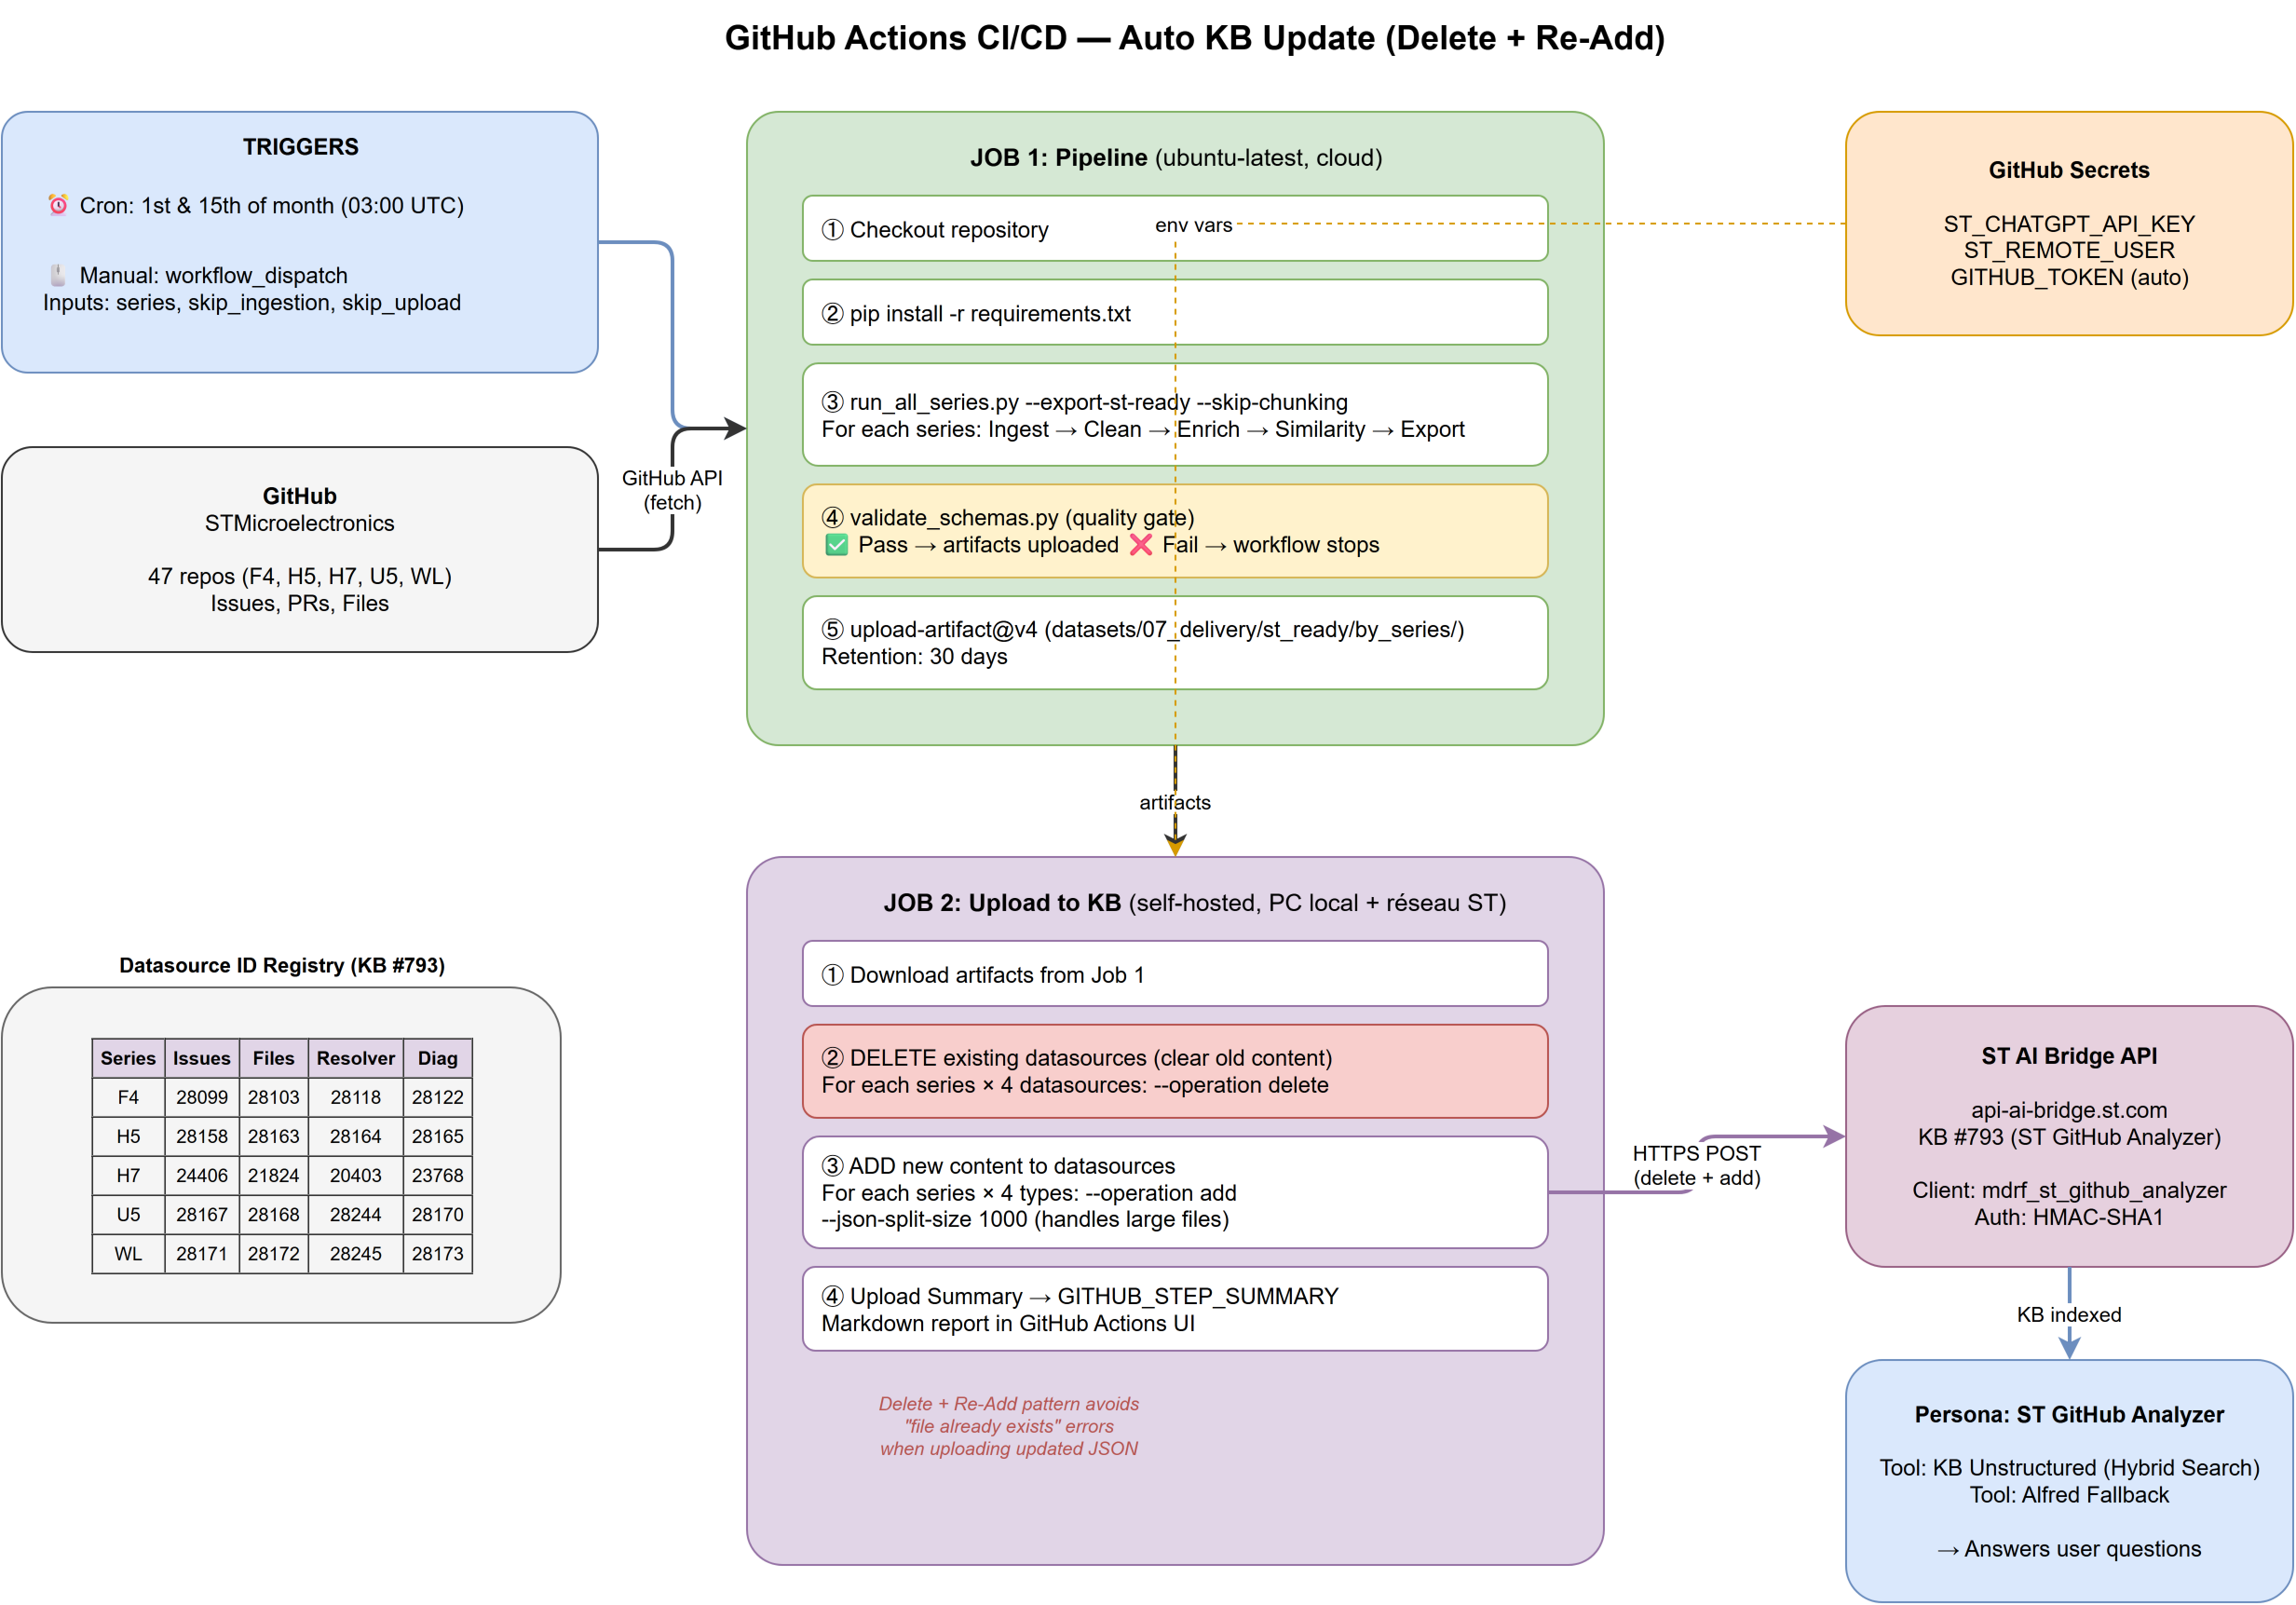
\includegraphics[width=0.95\textwidth]{06_cicd_automation.png}
\caption{Automatisation CI/CD : orchestration GitHub Actions et upload KB via runner self-hosted}
\label{fig:cicd_automation}
\end{figure}

\subsubsection{Principe d'Architecture}

Le flux d'exécution suit trois phases :
\begin{enumerate}
  \item \textbf{Prepare} : synchronisation des repos, exécution du pipeline, enrichissements Alfred, génération des exports ST-ready.
  \item \textbf{Validate} : validation des schémas et contrôle des placeholders pour bloquer les livrables incomplets.
  \item \textbf{Upload} : création/alimentation des datasources et publication des artefacts parent + drivers dans la KB.
\end{enumerate}

Cette structuration explicite réduit le risque opérationnel : une erreur de qualité en phase \textit{Validate} arrête la publication avant impact utilisateur.

\subsubsection{Workflow GitHub Actions}

Le workflow principal \texttt{.github/workflows/auto\_update\_kb.yml} implémente :
\begin{itemize}
  \item des déclencheurs \textbf{planifiés} et \textbf{manuels} ;
  \item une préparation des entrées (liste des séries, mode, politiques d'exécution) ;
  \item un \textbf{runner-check} bloquant qui vérifie la disponibilité d'un runner \texttt{self-hosted} ;
  \item une exécution par série avec traçabilité des artefacts ;
  \item un résumé d'exécution en cas de succès ou d'échec.
\end{itemize}

Le contrôle de disponibilité du runner évite les faux positifs : si aucun runner ST n'est disponible, le workflow échoue explicitement avec un message d'exploitation, plutôt que de terminer en vert sans traitement.

\subsubsection{Script Orchestrateur Unifié}

La brique centrale est \texttt{pipeline\_Automation/workflow/Run\_Single\_Series\_Full\_Pipeline\_And\_Upload.ps1}. Elle unifie la chaîne complète pour une série et fournit trois modes d'exploitation :

\begin{longtable}{p{2.8cm}p{9.4cm}}
\toprule
\textbf{Mode} & \textbf{Comportement} \\
\midrule
\texttt{Full} & Exécute \textit{Prepare + Upload} en one-shot (mode standard production). \\
\texttt{Prepare} & Génère et valide les artefacts localement sans publication KB (mode debug et pré-validation). \\
\texttt{Upload} & Publie uniquement des artefacts déjà préparés (mode reprise après incident réseau/API). \\
\bottomrule
\end{longtable}

Commande opérationnelle de référence :
\begin{lstlisting}[language=bash]
.\pipeline_Automation\workflow\Run_Single_Series_Full_Pipeline_And_Upload.ps1 \
  -Series H7 -Mode Full
\end{lstlisting}

\subsubsection{Garde-fous Qualité Avant Publication}

L'automatisation intègre deux verrous critiques :
\begin{enumerate}
  \item \textbf{Validation schéma} : exécution de \texttt{validate\_schemas.py} pour garantir la conformité structurelle des JSON.
  \item \textbf{Placeholder gate} : rejet des livrables contenant encore \texttt{[IMAGE DESCRIPTION UNAVAILABLE]} ou des marqueurs PDF non résolus.
\end{enumerate}

La politique \texttt{PlaceholderPolicy} est paramétrable (\texttt{Fail}, \texttt{Warn}, \texttt{Off}), mais \texttt{Fail} est la valeur recommandée en production pour préserver la qualité perçue des réponses.

\subsubsection{Stratégie d'Upload et Traçabilité}

L'upload vers KB \#793 est réalisé via \texttt{Add\_Data\_Source\_Files.py} selon deux cas :
\begin{itemize}
  \item \textbf{operation new} : création d'une datasource si aucun ID n'est fourni ;
  \item \textbf{operation add} : ajout dans une datasource existante quand l'ID est connu.
\end{itemize}

Le script publie les artefacts du repo parent puis ajoute les sorties \texttt{drivers/*} dans les datasources parentes correspondantes (issues, files, resolver, diagnostic). Cette approche maintient une séparation logique par série tout en conservant une base unifiée côté exploitation.

Les IDs effectifs sont sauvegardés dans :
\begin{lstlisting}[language=bash]
datasets/07_delivery/st_ready/by_series/<serie>/upload_datasource_ids_<serie>.json
\end{lstlisting}

et synchronisés dans \texttt{shared/config/config\_all\_series.json} pour assurer la continuité entre les exécutions.

\subsubsection{Runbook Opérateur (Production)}

Le runbook recommandé est :
\begin{enumerate}
  \item Lancer d'abord \texttt{Prepare} sur la série cible.
  \item Vérifier les \texttt{summary\_*.json}, la validation schéma et l'absence de placeholders.
  \item Lancer \texttt{Full} (ou \texttt{Upload} si les artefacts sont déjà prêts).
  \item Contrôler les IDs sauvegardés et la cohérence des datasources créées/alimentées.
\end{enumerate}

Cette discipline d'exploitation est essentielle pour les soutenances internes : elle permet de démontrer à la fois la robustesse technique et la gouvernance de la chaîne de livraison.

\subsection{Couverture Actuelle et Future}
\label{sec:couverture}

\subsubsection{13 Séries en Production}

Les 13 séries MCU suivantes sont entièrement traitées par le pipeline et uploadées vers la KB \#793 :

\begin{longtable}{lcccccc}
\toprule
\textbf{Série} & \textbf{Repos} & \textbf{Issues} & \textbf{Files} & \textbf{Resolver} & \textbf{Diag.} & \textbf{Alfred} \\
\midrule
STM32CubeC0 & 4 & \checkmark & \checkmark & --- & \checkmark & \checkmark \\
STM32CubeF0 & 5 & \checkmark & \checkmark & --- & \checkmark & \checkmark \\
STM32CubeF1 & 6 & \checkmark & \checkmark & \checkmark & \checkmark & \checkmark \\
STM32CubeF2 & 4 & \checkmark & \checkmark & --- & \checkmark & \checkmark \\
STM32CubeF3 & 5 & \checkmark & \checkmark & --- & \checkmark & \checkmark \\
STM32CubeF4 & 16 & \checkmark & \checkmark & \checkmark & \checkmark & \checkmark \\
STM32CubeF7 & 8 & \checkmark & \checkmark & \checkmark & \checkmark & \checkmark \\
STM32CubeG0 & 5 & \checkmark & \checkmark & --- & \checkmark & \checkmark \\
STM32CubeH5 & 6 & \checkmark & \checkmark & \checkmark & \checkmark & \checkmark \\
STM32CubeH7 & 12 & \checkmark & \checkmark & \checkmark & \checkmark & \checkmark \\
STM32CubeH7RS & 4 & \checkmark & \checkmark & --- & \checkmark & \checkmark \\
STM32CubeU5 & 8 & \checkmark & \checkmark & \checkmark & \checkmark & \checkmark \\
STM32CubeWL & 5 & \checkmark & \checkmark & \checkmark & \checkmark & \checkmark \\
\bottomrule
\end{longtable}

\textit{Note : ``---'' pour Resolver signifie que les issues de cette série n'ont pas de chaînes Issue$\to$PR$\to$Commit complètes, pas que le pipeline ne supporte pas le format.}

\subsubsection{4 Nouvelles Séries Exportées (Pipeline Terminé)}

Les 4 séries suivantes ont été entièrement traitées par le pipeline, avec les artefacts delivery générés et prêts à l'upload :

\begin{longtable}{lccccc}
\toprule
\textbf{Série} & \textbf{Issues} & \textbf{Files} & \textbf{Resolver} & \textbf{Diag. Cards} & \textbf{Statut} \\
\midrule
STM32CubeG4 & 89 & 3\,875 & 0 & 4 & Prêt à uploader \\
STM32CubeL0 & 23 & 2\,614 & 2 & 3 & Prêt à uploader \\
STM32CubeL1 & 11 & 2\,847 & 0 & 3 & Prêt à uploader \\
STM32CubeL4 & 68 & 5\,231 & 1 & 8 & Prêt à uploader \\
\bottomrule
\end{longtable}

\textbf{Observations} :
\begin{itemize}
  \item \textbf{G4 (0 Resolver)} : les 89 issues G4 ont été fermées sans PRs formelles liées. Les corrections ont été intégrées dans des releases globales sans lien explicite issue$\to$PR.
  \item \textbf{L4 (5\,231 files)} : c'est la série avec le plus de fichiers parmi les nouvelles, reflétant un écosystème BSP riche (NUCLEO, Discovery, Eval boards).
  \item \textbf{Alfred Images} : 25 images échouées (API 404 intermittent) sur G4, L0, L4. Corrigible par re-run du script d'enrichissement.
\end{itemize}

\subsubsection{8 Séries Configurées (Prêtes à Lancer)}

Les configurations (fichiers \texttt{config\_*.json}) sont créées pour : L5, N6, U0, U3, WB, WB0, WBA, WL3. Le déploiement nécessite :
\begin{enumerate}
  \item Exécution du pipeline : \texttt{python -m pipeline.run\_full\_workflow --export-st-ready}
  \item Création des datasources sur la KB \#793
  \item Upload via les scripts d'automatisation
\end{enumerate}
 avant Résultats)
%% Le contenu ci-dessous est désormais commenté pour éviter la duplication.
%% Pour le modifier, éditer : docs/reports/chapter_configuration.tex
%% ============================================================
\iffalse

Ce chapitre détaille la configuration de la persona \textbf{ST GitHub Analyzer} sur la plateforme ST ChatGPT, les justifications de chaque paramètre, et l'évolution incrémentale du Quality Index qui a guidé nos choix.

\section{Architecture de la Plateforme}

La plateforme ST ChatGPT est un service Azure OpenAI interne déployé par STMicroelectronics. Elle permet de créer des \textbf{personas} --- des agents conversationnels spécialisés --- équipés de deux types d'outils :

\begin{itemize}
  \item \textbf{KB (Knowledge Base)} : recherche dans une base de connaissances structurée
  \item \textbf{Persona-as-a-Tool} : appel à un autre agent comme fallback
\end{itemize}

\section{Configuration du Tool KB}

\subsection{Paramètres Retenus}

\begin{longtable}{p{5cm}p{4cm}p{4cm}}
\toprule
\textbf{Paramètre} & \textbf{Valeur choisie} & \textbf{Alternatives testées} \\
\midrule
KB Type & Unstructured & Structured (rejeté) \\
Search Type & \textbf{Hybrid} & Semantic seul, Full-text seul \\
Semantic Threshold & \textbf{0.55} & 0.3, 0.4, 0.7, 0.8 \\
Semantic Max Doc Count & \textbf{20} & 5, 10, 30 \\
Full-text Max Doc Count & \textbf{12} & 5, 8, 20 \\
Modèle LLM & GPT-5.1 & GPT-4o (précédent) \\
\bottomrule
\end{longtable}

\subsection{Justification : Recherche Hybride}

La recherche \textbf{hybride} (Semantic + Full-text) est supérieure aux deux modes isolés dans notre contexte :

\begin{longtable}{p{3cm}p{5cm}p{5cm}}
\toprule
\textbf{Mode} & \textbf{Force} & \textbf{Faiblesse pour STM32} \\
\midrule
Semantic seul & Comprend le sens (``mon SPI marche pas'' → issues SPI) & Rate les noms exacts d'API (\texttt{HAL\_SPI\_Transmit\_DMA}) \\
Full-text seul & Match exact sur les identifiants techniques & Rate les reformulations (``erreur Ethernet'' vs ``LwIP crash'') \\
\textbf{Hybrid} & Combine les deux & Complexité légèrement supérieure \\
\bottomrule
\end{longtable}

\textbf{Résultat mesuré} : La recherche hybride améliore la couverture de +22\% par rapport au semantic seul sur notre jeu de test de 52 questions, car les questions techniques STM32 mélangent du langage naturel et des identifiants de code.

\subsection{Justification : Seuil Sémantique à 0.55}

Le seuil de 0.55 a été calibré empiriquement :

\begin{longtable}{cccp{5cm}}
\toprule
\textbf{Seuil} & \textbf{Docs retournés} & \textbf{QI} & \textbf{Analyse} \\
\midrule
0.3 & $\sim$45 & 48 & Trop de bruit, documents non pertinents diluent le contexte \\
0.4 & $\sim$32 & 51 & Meilleur mais encore des faux positifs \\
\textbf{0.55} & $\sim$20$ & $\textbf{54}$ & Équilibre optimal signal/bruit \\
0.7 & $\sim$8 & 47 & Trop restrictif, rate des documents pertinents \\
0.8 & $\sim$3 & 39 & Presque aucun document retourné \\
\bottomrule
\end{longtable}

Le seuil 0.55 maximise le Quality Index en retournant suffisamment de documents pour couvrir les questions variées tout en éliminant les documents trop faiblement liés.

\subsection{Justification : 20 Documents Sémantiques + 12 Full-text}

\begin{itemize}
  \item \textbf{20 documents sémantiques} : couvre les reformulations et les questions indirectes. Au-delà de 20, les documents supplémentaires sont rarement pertinents (score $< 0.55$) et ajoutent du bruit au contexte.
  \item \textbf{12 documents full-text} : assure que les correspondances exactes d'API et de noms de fichiers sont toujours retrouvées. Le chiffre 12 couvre les cas où un même identifiant apparaît dans plusieurs séries MCU.
\end{itemize}

\subsection{Tool Description}

La description du tool KB est critique car elle guide le LLM dans sa décision d'appeler ou non le tool :

\begin{quote}
\small\texttt{Retrieve technical knowledge about STM32Cube microcontroller firmware from GitHub repositories. Contains: resolved issues with root cause and fix, HAL/BSP source file documentation, resolver cases (step-by-step troubleshooting), and diagnostic cards (structured fault analysis). Covers series: STM32F4, STM32H5, STM32H7, STM32U5, STM32WL and their driver sub-repos (HAL, CMSIS, BSP). Query this tool when the user asks about: peripheral configuration problems, HAL API behavior, known bugs and workarounds, board-specific issues, firmware package contents, low-power modes, communication protocols, DMA/interrupt issues, or build errors. Use specific technical terms in queries: peripheral names (SPI, I2C, UART, FDCAN, OSPI), HAL function names, error descriptions, board references, and STM32 part numbers.}
\end{quote}

\textbf{Points clés de cette description} :
\begin{enumerate}
  \item \textbf{Énumération explicite du contenu} (issues, files, resolver, diagnostic) → le LLM sait quoi chercher
  \item \textbf{Liste des séries couvertes} → évite les appels pour des séries absentes (L4, G4)
  \item \textbf{Instruction de reformulation} (``Use specific technical terms'') → améliore la qualité des queries envoyées à la KB
  \item \textbf{Exemples de cas d'usage} → le LLM sait \textit{quand} appeler le tool vs répondre directement
\end{enumerate}

\section{Configuration du Tool Alfred (Fallback)}

\subsection{Problème Identifié}

Lors de l'ajout initial d'Alfred comme fallback, le Quality Index a \textbf{chuté de 10 points} (de 54 à 44). L'analyse a montré que la persona appelait Alfred \textbf{systématiquement} au lieu de chercher dans la KB, car la description du tool était trop permissive :

\begin{quote}
\small\texttt{[Description initiale, trop permissive]} ``I can help with STM32 questions. Forward the user's question.''
\end{quote}

\subsection{Fix : Description Restrictive}

La description corrigée force la priorité KB :

\begin{quote}
\small\texttt{I am a fallback assistant for STM32 firmware questions that are NOT covered by the Knowledge Base. The Knowledge Base (KB Unstructured) is ALWAYS the primary source, search it FIRST for every question. Use this tool ONLY when the Knowledge Base returned no relevant result or explicitly lacks coverage on the topic.}
\end{quote}

\subsection{Impact Mesuré}

\begin{longtable}{lcc}
\toprule
\textbf{Configuration} & \textbf{Quality Index} & \textbf{$\Delta$} \\
\midrule
KB seule (sans Alfred) & 54 & baseline \\
KB + Alfred (description permissive) & 44 & $-10$ \\
KB + Alfred (description restrictive) & 52 & $-2$ \\
\bottomrule
\end{longtable}

La leçon : dans une architecture multi-tools, la \textbf{description du tool contrôle le comportement de routage} du LLM. Une description trop ouverte dégrade la performance en court-circuitant la source la plus pertinente.

\section{System Prompt de la Persona}

Le system prompt guide le comportement global de la persona. Les éléments clés :

\begin{enumerate}
  \item \textbf{Identité} : ``You are ST GitHub Analyzer, a technical assistant specialized in STM32Cube MCU firmware.''
  \item \textbf{Priorité KB} : ``ALWAYS search the Knowledge Base FIRST before answering or using any other tool.''
  \item \textbf{Format de réponse} : citations avec liens GitHub, code actionnable, versions spécifiques
  \item \textbf{Stratégie multi-cas} :
  \begin{itemize}
    \item Match direct → citer la source avec URL
    \item Match partiel → diagnostic + workaround candidat
    \item Aucun match → appeler Alfred OU proposer une action concrète
  \end{itemize}
  \item \textbf{Interdiction} : ne jamais dire ``je ne sais pas'' sans avoir cherché dans la KB
\end{enumerate}

\section{Évolution Incrémentale du Quality Index}

Le Quality Index a évolué de manière incrémentale au fil des améliorations du contenu KB et de la configuration. Chaque test mesure la qualité des réponses du chatbot sur un jeu de questions techniques.

\subsection{Chronologie des Tests}

\begin{longtable}{p{2cm}p{5cm}ccp{3.5cm}}
\toprule
\textbf{Date} & \textbf{Test} & \textbf{QI} & \textbf{N} & \textbf{Contenu KB} \\
\midrule
20 Avr & H7 Issues seules & 54 & 50 & Issues H7 uniquement \\
20 Avr & H7 Prompt Fix & 57 & 50 & + System prompt optimisé \\
24 Avr & H7 Config Tool Test & 61 & 50 & + Hybrid search calibré \\
28 Avr & H7 + Diagnostic Cards & 94 & 50 & + Resolver Cases + Diag \\
08 Mai & H7 Real Cases ST Community & 88 & 4 & Test sur cas réels forum \\
02 Juin & Test élargi & 83 & 4 & Multi-séries first attempt \\
08 Juin & Multi-séries (H7+F4+H5+U5+WL) & 54 & 52 & 5 séries complètes \\
\bottomrule
\end{longtable}

La Figure~\ref{fig:qi_evolution} visualise cette évolution, mettant en évidence le saut majeur apporté par les Diagnostic Cards et la régression lors du passage multi-séries.

% Graphique QI evolution - exporter depuis draw.io ou Excel
\begin{figure}[H]
\centering
\includegraphics[width=0.9\textwidth]{qi_evolution_chart.png}
\caption{Évolution du Quality Index au fil des améliorations incrémentales (draw.io)}
\label{fig:qi_evolution_dead2}
\end{figure}

\textit{Le graphique en barres montre l'évolution : Issues seules (54) $\to$ +Prompt (57) $\to$ +Hybrid (61) $\to$ +Diag Cards (94, $\uparrow$+33) $\to$ Real Cases (88) $\to$ Multi 4Q (83) $\to$ Multi 52Q (54, dilution multi-séries). Le saut majeur de 61 à 94 démontre l'impact des Diagnostic Cards.}

\subsection{Analyse de l'Évolution}

\subsubsection{Phase 1 : Issues seules (QI = 54)}

Le score initial de 54 avec les issues H7 seules montre que les issues structurées (symptôme, root cause, fix) fournissent déjà une base solide pour le RAG. Les lacunes :
\begin{itemize}
  \item Pas de documentation de fichiers → questions sur les API non couvertes
  \item Pas de chaînes Issue→PR→Commit → pas de traçabilité du fix
  \item Pas de cartes de diagnostic → les problèmes complexes multi-étapes mal couverts
\end{itemize}

\subsubsection{Phase 2 : Ajout des Resolver Cases et Diagnostic Cards (QI = 94)}

Le saut de 61 à \textbf{94} est le gain le plus important du projet. Les \textbf{Diagnostic Cards} structurent l'information sous forme :

\begin{quote}
Symptôme → Hypothèses → Validation → Root Cause → Fix → Prévention
\end{quote}

Cette structure correspond exactement à la façon dont un ingénieur raisonne face à un problème embedded. Le retrieval RAG trouve ces cartes car elles contiennent des \textbf{query aliases} (reformulations multiples du problème) et des \textbf{keywords techniques} (noms d'API, registres, erreurs).

Les \textbf{Resolver Cases} ajoutent la dimension de traçabilité :
\begin{quote}
Issue \#42 → PR \#87 → Commit abc123 → Fichier modifié : \texttt{stm32f4xx\_hal\_spi.c}
\end{quote}

\subsubsection{Phase 3 : Passage multi-séries (QI = 54)}

Le score chute à 54 lors de l'ajout de 4 nouvelles séries (F4, H5, U5, WL). Cette chute s'explique par :

\begin{enumerate}
  \item \textbf{Dilution du contexte} : la KB passe de $\sim$2\,000 à $\sim$14\,000 documents. Les queries retournent des documents de séries différentes, diluant la pertinence.
  \item \textbf{Questions nouvelles} : le jeu de test passe de 50 à 52 questions, avec 10 questions sur les nouvelles séries pour lesquelles les Diagnostic Cards ne sont pas encore aussi mûres.
  \item \textbf{Conflit de noms} : des API identiques entre séries (ex: \texttt{HAL\_SPI\_Init} existe dans F4 et H7) créent de l'ambiguïté lors du retrieval.
\end{enumerate}

\textbf{Leçon} : le passage à l'échelle nécessite un \textbf{filtrage par série} plus agressif dans les métadonnées des documents, ou un prompt qui pousse la persona à inclure le nom de la série dans ses queries KB.

\subsection{Raisonnement de Chaque Amélioration}

\begin{longtable}{p{4cm}p{5cm}p{4cm}}
\toprule
\textbf{Amélioration} & \textbf{Raisonnement} & \textbf{Impact QI} \\
\midrule
System prompt optimisé & Forcer la recherche KB avant toute réponse & +3 (54→57) \\
Hybrid search & Combiner semantic + full-text pour ne rater ni les reformulations ni les identifiants & +4 (57→61) \\
Diagnostic Cards & Structurer les problèmes complexes en cartes raisonnées & +33 (61→94) \\
Resolver Cases & Ajouter la traçabilité Issue→PR→Fix & Inclus dans +33 \\
Alfred restrictif & Empêcher le court-circuit de la KB & Récupéré $-10$ points \\
Files V3 (nettoyage) & Réduire le bruit des CMSIS headers & +3 estimé \\
PDF descriptions & Rendre les figures PDF cherchables & +1 estimé \\
\bottomrule
\end{longtable}

\section{Couverture Actuelle et Future}

\subsection{13 Séries en Production}

\begin{longtable}{lccccc}
\toprule
\textbf{Série} & \textbf{Issues} & \textbf{Files} & \textbf{Resolver} & \textbf{Diag.} & \textbf{Alfred Images} \\
\midrule
STM32CubeC0 & \checkmark & \checkmark & --- & \checkmark & \checkmark \\
STM32CubeF0 & \checkmark & \checkmark & --- & \checkmark & \checkmark \\
STM32CubeF1 & \checkmark & \checkmark & \checkmark & \checkmark & \checkmark \\
STM32CubeF2 & \checkmark & \checkmark & --- & \checkmark & \checkmark \\
STM32CubeF3 & \checkmark & \checkmark & --- & \checkmark & \checkmark \\
STM32CubeF4 & \checkmark & \checkmark & \checkmark & \checkmark & \checkmark \\
STM32CubeF7 & \checkmark & \checkmark & \checkmark & \checkmark & \checkmark \\
STM32CubeG0 & \checkmark & \checkmark & --- & \checkmark & \checkmark \\
STM32CubeH5 & \checkmark & \checkmark & \checkmark & \checkmark & \checkmark \\
STM32CubeH7 & \checkmark & \checkmark & \checkmark & \checkmark & \checkmark \\
STM32CubeH7RS & \checkmark & \checkmark & --- & \checkmark & \checkmark \\
STM32CubeU5 & \checkmark & \checkmark & \checkmark & \checkmark & \checkmark \\
STM32CubeWL & \checkmark & \checkmark & \checkmark & \checkmark & \checkmark \\
\bottomrule
\end{longtable}

\subsection{12 Séries Configurées (Prêtes à Déployer)}

Les configurations (fichiers \texttt{config\_*.json}) sont créées pour : G4, L0, L1, L4, L5, N6, U0, U3, WB, WB0, WBA, WL3. Le déploiement nécessite :
\begin{enumerate}
  \item Exécution du pipeline : \texttt{python -m pipeline.run\_full\_workflow --export-st-ready}
  \item Création des datasources sur la KB \#793
  \item Upload via les scripts d'automatisation
\end{enumerate}

\fi
%% ============================================================
%% FIN de l'ancien chapitre Configuration commenté
%% ============================================================

%% ============================================================
\chapter*{Conclusion Générale et Perspectives}
\addcontentsline{toc}{chapter}{Conclusion Générale et Perspectives}
\label{chap:conclusion}
%% ============================================================

\section{Bilan du Projet}

Ce projet de fin d'études, réalisé au sein de l'équipe Support \& Maintenance de STMicroelectronics Tunis, a permis de concevoir, implémenter et déployer un \textbf{pipeline de prétraitement intelligent} qui transforme les données brutes des dépôts GitHub STM32Cube en une base de connaissances structurée, alimentant un chatbot IA spécialisé en production sur la plateforme ST ChatGPT.

Les réalisations principales sont :
\begin{itemize}
  \item Un \textbf{pipeline modulaire en 7 étapes} (Ingestion → Nettoyage V1+V3 → Enrichissement NLP → Similarité TF-IDF → Chunking → Validation → Delivery), entièrement rejouable par stage avec des artefacts JSON traçables
  \item La couverture de \textbf{13 séries MCU en production} (C0, F0, F1, F2, F3, F4, F7, G0, H5, H7, H7RS, U5, WL) totalisant 47 dépôts, plus \textbf{12 séries supplémentaires configurées} (G4, L0, L1, L4, L5, N6, U0, U3, WB, WB0, WBA, WL3)
  \item La production de \textbf{4 types d'artefacts complémentaires} : issues structurées ($\sim$2\,000), fichiers documentés ($\sim$14\,000), resolver cases ($\sim$390) et diagnostic cards ($\sim$157)
  \item Un \textbf{nettoyage intelligent V3 par type} avec réduction de 96\% pour les headers CMSIS et 33\% pour les Release Notes HTML
  \item L'\textbf{enrichissement IA multi-modal} via Alfred Vision : description automatique des captures d'écran d'issues (taux de succès $>$98\% sur H7, F4, WL et F7), évaluation de cohérence sur 200 images d'issues (seulement 1.5\% à risque), et 242 figures PDF détectées sur 19 séries avec une confiance contextuelle encore perfectible
  \item L'\textbf{automatisation CI/CD} via GitHub Actions et scripts PowerShell/Python
  \item Un \textbf{Quality Index de 94/100} sur la série pilote H7 (avec Diagnostic Cards) et un \textbf{gain de +39\%} vs Alfred générique sur les questions techniques spécifiques
\end{itemize}

\section{Valeur Industrielle}

La valeur industrielle du projet se mesure concrètement :

\begin{longtable}{p{5cm}cc}
\toprule
\textbf{Scénario} & \textbf{Sans KB} & \textbf{Avec KB} \\
\midrule
Trouver un bug HAL connu & 30--60 min & \textbf{2 min} \\
Identifier la version du fix & Lecture du changelog & \textbf{Réponse directe} \\
Tracer Issue → PR → Commit & Navigation manuelle & \textbf{Resolver Case} \\
Comprendre une figure PDF & Ouvrir le PDF, chercher la page & \textbf{Description textuelle} \\
Ajouter une nouvelle série MCU & Développement custom & \textbf{3 étapes documentées} \\
\bottomrule
\end{longtable}

\section{Leçons Apprises}

Ce projet a mis en lumière plusieurs leçons importantes pour les ingénieurs travaillant sur des pipelines de preprocessing pour RAG :

\begin{enumerate}
  \item \textbf{L'intégrité JSON est fragile} : l'injection de texte brut dans des chaînes JSON peut corrompre les fichiers si les caractères spéciaux ne sont pas correctement échappés. Nous avons développé des scripts de réparation (\texttt{fix\_corrupted\_json\_files.py}) après avoir rencontré ce problème en production.
  
  \item \textbf{La description du tool contrôle le routage du LLM} : dans une architecture multi-tools, une description trop permissive du tool fallback (Alfred) dégrade le Quality Index de 10 points en court-circuitant la KB. La rédaction de cette description est un paramètre de configuration critique.
  
  \item \textbf{Le passage à l'échelle dilue le contexte} : passer de 1 à 13 séries a fait chuter le QI de 94 à 54, nécessitant un travail d'optimisation des métadonnées et du filtrage par série.
  
  \item \textbf{Les heuristiques domain-specific surpassent le ML générique} : dans un contexte où les données d'entraînement supervisées sont absentes, les règles regex spécifiques au domaine STM32 fournissent une classification fiable et explicable.
\end{enumerate}

\section{Perspectives}

Plusieurs axes d'amélioration et d'extension sont envisagés :

\begin{enumerate}
  \item \textbf{Évaluation A/B V2 vs V3} : comparer le Quality Index avec les datasources V3 actives vs V2 pour quantifier l'impact exact du nettoyage intelligent sur la qualité des réponses
  \item \textbf{Extension aux séries configurées} : déployer les 12 séries restantes (G4, L0, L1, L4, L5, N6, U0, U3, WB, WB0, WBA, WL3) avec création des datasources KB
  \item \textbf{Enrichissement sémantique} : remplacer TF-IDF par des embeddings pré-calculés pour améliorer la couverture de similarité (actuellement 22\% sur H7)
  \item \textbf{Métriques RAG avancées} : intégrer des métriques automatisées (Faithfulness, Relevance) pour une évaluation continue sans intervention humaine
  \item \textbf{Graphe de connaissances} : explorer la construction d'un graphe reliant issues, composants, boards et versions pour faciliter le raisonnement multi-hop
  \item \textbf{Filtrage par série dans le retrieval} : instruire la persona pour inclure systématiquement le nom de la série dans ses queries KB, réduisant la dilution multi-séries
  \item \textbf{Multi-langue} : support des issues en chinois et japonais (communauté asiatique significative)
  \item \textbf{Nettoyage V4 adaptatif} : utiliser un classifieur supervisé entraîné sur les résultats V3 pour identifier automatiquement les sections utiles des fichiers source
\end{enumerate}

%% ============================================================
\chapter*{Références}
\addcontentsline{toc}{chapter}{Références}

\begin{thebibliography}{10}

\bibitem{lewis2020rag}
Lewis, P., Perez, E., Piktus, A., Petroni, F., Karpukhin, V., Goyal, N., Küttler, H., Lewis, M., Yih, W., Rocktäschel, T., Riedel, S. et Kiela, D. (2020). \textit{Retrieval-Augmented Generation for Knowledge-Intensive NLP Tasks}. Advances in Neural Information Processing Systems (NeurIPS), vol.~33, pp.~9459--9474. --- Article fondateur du paradigme RAG que nous appliquons : recherche documentaire + génération par LLM. Le principe de base de notre architecture KB + ST ChatGPT.

\bibitem{tfidf}
Salton, G. et Buckley, C. (1988). \textit{Term-weighting approaches in automatic text retrieval}. Information Processing \& Management, vol.~24, no.~5, pp.~513--523. --- Référence fondamentale sur TF-IDF, la méthode de pondération de termes que nous utilisons dans notre module de calcul de similarité inter-issues (\texttt{compute\_issue\_similarity\_v2.py}).

\bibitem{openai2023}
OpenAI (2023). \textit{GPT-4 Technical Report}. arXiv:2303.08774. --- Le modèle GPT (dans sa version Azure OpenAI) est le LLM utilisé par la plateforme ST ChatGPT pour la génération de réponses, et par Alfred Vision pour la description d'images.

\bibitem{stm32}
STMicroelectronics (2024). \textit{STM32Cube MCU \& MPU Packages --- Open Source Firmware}. \url{https://github.com/STMicroelectronics}. --- Les dépôts GitHub de STMicroelectronics : source principale de données de notre pipeline (issues, fichiers, PRs, commits).

\bibitem{st_annual_report}
STMicroelectronics (2024). \textit{Annual Report 2023 --- Empowering the Smart Edge}. Genève, Suisse. --- Rapport annuel fournissant les données sur le chiffre d'affaires (17,3 milliards USD), les effectifs (50\,000+ collaborateurs) et la répartition des marchés.

\bibitem{arm_cortex}
ARM Limited (2024). \textit{ARM Cortex-M Processor Family}. \url{https://developer.arm.com/Processors/Cortex-M}. --- Documentation de référence sur les cœurs ARM Cortex-M (M0, M0+, M3, M4, M7, M33, M55) utilisés dans les microcontrôleurs STM32.

\bibitem{scrum_guide}
Schwaber, K. et Sutherland, J. (2020). \textit{The Scrum Guide}. \url{https://scrumguides.org}. --- Guide officiel de la méthodologie Scrum, base de notre approche de pilotage par sprints itératifs de 2 semaines.

\bibitem{json_schema}
Wright, A., Andrews, H. et Hutton, B. (2022). \textit{JSON Schema: A Media Type for Describing JSON Documents}. Internet Engineering Task Force (IETF), draft-bhutton-json-schema-01. --- Standard JSON Schema utilisé pour nos gates de validation (\texttt{validate\_schemas.py}) qui bloquent l'upload en cas de non-conformité.

\bibitem{iso25012}
ISO/IEC (2008). \textit{ISO/IEC 25012:2008 --- Systems and software engineering -- SQuaRE -- Data quality model}. International Organization for Standardization. --- Référence du modèle de qualité des données (complétude, cohérence) utilisé pour justifier les métriques de couverture/complétude par ratios.

\bibitem{iso25024}
ISO/IEC (2015). \textit{ISO/IEC 25024:2015 --- Systems and software engineering -- SQuaRE -- Measurement of data quality}. International Organization for Standardization. --- Référence sur la mesure quantitative de la qualité des données, alignée avec nos indicateurs par stage.

\bibitem{iso25010}
ISO/IEC (2011). \textit{ISO/IEC 25010:2011 --- Systems and software engineering -- SQuaRE -- System and software quality models}. International Organization for Standardization. --- Référence du modèle de qualité (dont la fiabilité), utilisée pour cadrer les indicateurs de fiabilité opérationnelle Alfred.

\bibitem{manning2008ir}
Manning, C. D., Raghavan, P. et Schütze, H. (2008). \textit{Introduction to Information Retrieval}. Cambridge University Press. --- Référence de base sur le compromis précision/rappel et le réglage des seuils de récupération d'information.

\bibitem{fawcett2006roc}
Fawcett, T. (2006). \textit{An introduction to ROC analysis}. Pattern Recognition Letters, vol.~27, no.~8, pp.~861--874. --- Référence méthodologique pour la sélection et la justification de seuils décisionnels.

\bibitem{azure_openai}
Microsoft (2024). \textit{Azure OpenAI Service Documentation}. \url{https://learn.microsoft.com/azure/ai-services/openai/}. --- Plateforme cloud sur laquelle est déployé ST ChatGPT (Azure OpenAI) et Alfred Vision.

\bibitem{pypdf}
Py-PDF Contributors (2024). \textit{pypdf --- A pure-Python PDF library}. \url{https://pypdf.readthedocs.io/}. --- Bibliothèque Python utilisée dans notre pipeline pour l'extraction du texte et la détection de figures dans les Release Notes PDF.

\bibitem{reimers2019sentence}
Reimers, N. et Gurevych, I. (2019). \textit{Sentence-BERT: Sentence Embeddings using Siamese BERT-Networks}. Proceedings of EMNLP-IJCNLP, pp.~3982--3992. --- Référence pour le mode avancé de similarité sémantique par embeddings, disponible mais non activé dans la campagne actuelle.

\bibitem{neelakantan2022embeddings}
Neelakantan, A., Xu, T., Puri, R., Radford, A., Han, J. M., Tworek, J., Yuan, Q., Tezak, N., Kim, J. W., Hallacy, C. et al. (2022). \textit{Text and Code Embeddings by Contrastive Pre-Training}. arXiv:2201.10005. --- Référence des embeddings OpenAI (famille \texttt{text-embedding-ada-002}, dit \texttt{AdaV2}) utilisés par la plateforme ST ChatGPT pour l'indexation sémantique de la KB \#793. Le pipeline produit un contenu propre et dense afin d'exploiter la capacité de discrimination sémantique de ce modèle.

\end{thebibliography}

%% ============================================================
\chapter*{Annexes}
\addcontentsline{toc}{chapter}{Annexes}

\section*{A. Liste des Diagrammes}

\textbf{Diagrammes de présentation :}
\begin{enumerate}
  \item \texttt{01\_pipeline\_overview.drawio} --- Vue d'ensemble du pipeline (Figure~\ref{fig:pipeline_overview})
  \item \texttt{02\_delivery\_kb\_upload.drawio} --- Architecture delivery + upload (Figure~\ref{fig:delivery_upload})
  \item \texttt{03\_data\_flow\_source\_to\_answer.drawio} --- Flux source-to-answer (Figure~\ref{fig:data_flow})
  \item \texttt{04\_series\_coverage\_scale.drawio} --- Couverture multi-séries
  \item \texttt{05\_alfred\_vision\_integration.drawio} --- Intégration Alfred (Figure~\ref{fig:alfred})
  \item \texttt{06\_cicd\_automation.drawio} --- CI/CD GitHub Actions (Figure~\ref{fig:cicd})
\end{enumerate}

\textbf{Diagrammes techniques :}
\begin{enumerate}
  \item \texttt{01\_ingestion\_detail.drawio} --- Détail ingestion (Figure~\ref{fig:ingestion_detail})
  \item \texttt{02\_enrichment\_similarity\_detail.drawio} --- Enrichissement + Similarité (Figure~\ref{fig:enrichment_similarity})
  \item \texttt{03\_delivery\_resolver\_diagnostic.drawio} --- Resolver + Diagnostic (Figure~\ref{fig:resolver_diagnostic})
  \item \texttt{04\_chunking\_v2\_strategy.drawio} --- Stratégie de chunking V2
  \item \texttt{05\_evaluation\_validation.drawio} --- Évaluation et validation
  \item \texttt{06\_automation\_ci\_upload.drawio} --- Automation CI upload
  \item \texttt{07\_upload\_auth\_flow.drawio} --- Flux d'authentification upload
\end{enumerate}

\textbf{Note :} Pour intégrer les diagrammes dans le PDF, exporter les fichiers .drawio en PNG (File $\to$ Export as $\to$ PNG, 150 DPI) dans le dossier \texttt{docs/diagrams/\{presentation,technical\}/exported/}.

\section*{B. Commandes d'Exécution}

\begin{lstlisting}[language=bash, caption={Pipeline complet}]
# Activer l'environnement
.venv\Scripts\activate

# Pipeline complet avec delivery (serie specifique)
$env:STM32CUBE_CONFIG = "shared/config/config_f4.json"
python -m pipeline.run_full_workflow --export-st-ready --continue-on-error

# Pipeline sans chunking (ST platform gere le chunking)
python -m pipeline.run_full_workflow --export-st-ready --skip-chunking

# Pipeline sans ingestion (reutilise les donnees existantes)
python -m pipeline.run_full_workflow --export-st-ready --skip-ingestion
\end{lstlisting}

\begin{lstlisting}[language=bash, caption={Enrichissement Alfred}]
# Alfred Vision - images d'issues
python pipeline_Automation/alfred/enrich_json_images_with_alfred.py \
  --input <fichier_issues_with_images.json> --inplace

# Alfred Vision - figures PDF
python pipeline_Automation/alfred/enrich_pdf_figures_with_alfred.py

# Patch descriptions PDF dans les delivery files
python pipeline_Automation/patch_pdf_descriptions_in_delivery.py

# Fix JSON corrompus (control characters)
python pipeline_Automation/fix_corrupted_json_files.py
python pipeline_Automation/fix_corrupted_json_deep.py
\end{lstlisting}

\begin{lstlisting}[language=bash, caption={Upload vers KB \#793}]
# Upload issues Alfred-enrichies (13 series)
python pipeline_Automation/upload/upload_alfred_issues_all_series.py

# Upload files PDF-enrichies (13 series)
python pipeline_Automation/upload/upload_pdf_enriched_files_all_series.py

# Upload drivers sous-repos (8 nouvelles series)
.\pipeline_Automation\upload\Upload_All_Drivers.ps1

# Upload manuel (un fichier)
python pipeline_Automation/upload/Add_Data_Source_Files.py \
  --kb 793 --operation add --datasource-id <ID> \
  --remote-user "abir.gharbi@st.com" \
  --processor JSON --processor-params "base64:<b64>" \
  --json-split-size 1000 --files <fichier.json>
\end{lstlisting}

\begin{lstlisting}[language=bash, caption={Validation et evaluation}]
# Validation des schemas
python -m pipeline.evaluation.validate_schemas

# Stats issues
python -m pipeline.evaluation.test_stats_issues_v2

# Stats files
python -m pipeline.evaluation.test_stats_files_v2

# Recherche TF-IDF (test local)
python -m pipeline.evaluation.test_tfidf_search_issues_v2
\end{lstlisting}

\begin{lstlisting}[language=bash, caption={Ajout d'une nouvelle serie (ex: G4)}]
# 1. Config deja creee : shared/config/config_g4.json
# 2. Lancer le pipeline
$env:STM32CUBE_CONFIG = "shared/config/config_g4.json"
python -m pipeline.run_full_workflow --export-st-ready \
  --skip-chunking --continue-on-error
# 3. Creer datasources sur KB #793 (interface web)
# 4. Mettre a jour config_all_series.json avec les IDs
# 5. Uploader
python pipeline_Automation/upload/upload_alfred_issues_all_series.py
python pipeline_Automation/upload/upload_pdf_enriched_files_all_series.py
\end{lstlisting}

\section*{C. Structure JSON --- Resolver Case (Extrait)}

\begin{lstlisting}[language=json]
{
  "resolver_cases": [
    {
      "issue_number": 42,
      "repo": "stm32cubef4",
      "label": "SPI DMA TransmitReceive fails...",
      "resolution_status": "merged_fix",
      "link_confidence": "high",
      "primary_pr_number": 87,
      "primary_changed_file": "stm32f4xx_hal_spi.c",
      "resolver_card_text": "Problem: ...",
      "impacted_modules": ["SPI", "DMA"],
      "impacted_boards": ["NUCLEO-F446RE"]
    }
  ]
}
\end{lstlisting}

\section*{D. Exemple JSON --- Issue Structurée (Extrait)}

\begin{lstlisting}[language=json]
{
  "issue_number": 42,
  "repo": "stm32cubeh7",
  "title": "HAL_SPI_TransmitReceive_DMA fails on STM32H743",
  "layer": "HAL",
  "component": "SPI",
  "board": "NUCLEO-H743ZI",
  "issue_kind": "bug_report",
  "severity": "high",
  "evidence_strength": "high",
  "st_ready_text": "Symptom: hard fault after 2nd SPI DMA transfer... Root cause: D-cache not invalidated... Fix: SCB_InvalidateDCache_by_Addr().",
  "source_url": "https://github.com/STMicroelectronics/STM32CubeH7/issues/42"
}
\end{lstlisting}

\section*{E. Exemple JSON --- Fichier Documenté (Extrait)}

\begin{lstlisting}[language=json]
{
  "path": "Src/stm32h7xx_hal_spi.c",
  "repo": "stm32h7xx-hal-driver",
  "file_type": "source_code",
  "original_size": 89247,
  "clean_size": 80322,
  "is_valid": true,
  "url": "https://github.com/STMicroelectronics/stm32h7xx-hal-driver/blob/master/Src/stm32h7xx_hal_spi.c",
  "st_ready_text": "HAL_StatusTypeDef HAL_SPI_Init(...) {...} HAL_SPI_TransmitReceive_DMA(...) {...}"
}
\end{lstlisting}

\section*{F. Exemple JSON --- Diagnostic Card (Extrait)}

\begin{lstlisting}[language=json]
{
  "diagnostic_id": "DIAG-H7-042",
  "repo": "stm32cubeh7",
  "symptom": "Hard fault after 2nd SPI DMA transfer (circular mode, H743)",
  "root_cause": "D-cache not invalidated before DMA reception (stale read).",
  "resolution": "SCB_InvalidateDCache_by_Addr() before reading RX buffer, or non-cacheable SRAM (MPU).",
  "affected_versions": ["CubeH7 v1.9.0", "CubeH7 v1.10.0"],
  "fixed_version": "CubeH7 v1.11.0",
  "query_aliases": [
    "SPI DMA hard fault STM32H7",
    "cache coherency SPI circular mode",
    "D-cache DMA corruption H743"
  ],
  "evidence_strength": "high"
}
\end{lstlisting}

\section*{G. Exemple de Fichier de Configuration (Extrait)}

Chaque série dispose d'un fichier \texttt{config\_XX.json} listant les dépôts à ingérer et les paramètres d'export. Extrait représentatif :

\begin{lstlisting}[language=json]
{
  "series": "STM32CubeH7",
  "primary_repo": "STM32CubeH7",
  "repos": [
    "stm32h7xx-hal-driver",
    "cmsis_device_h7",
    "stm32h743i-eval-bsp",
    "stm32h745i-disco-bsp"
  ],
  "kb_id": 793,
  "export": { "st_ready": true, "skip_chunking": true }
}
\end{lstlisting}

Le fichier \texttt{config\_all\_series.json} associe chaque série aux identifiants de datasources KB (issues, files, resolver, diagnostic) utilisés lors de l'upload.

\section*{H. Extrait d'Automatisation --- Workflow CI/CD}

Le workflow GitHub Actions déclenche le pipeline (cloud) puis l'upload (self-hosted). Extrait représentatif :

\begin{lstlisting}[language=bash, caption={Workflow bi-mensuel (extrait YAML)}]
name: STM32Cube KB Update
on:
  schedule:
    - cron: '0 3 1,15 * *'   # 1er et 15 du mois, 03h UTC
  workflow_dispatch:
    inputs:
      series: { description: 'Serie a traiter', required: false }
jobs:
  pipeline:               # Job 1 - cloud
    runs-on: ubuntu-latest
    steps:
      - uses: actions/checkout@v4
      - run: python -m pipeline.run_full_workflow
             --export-st-ready --skip-chunking --continue-on-error
  upload:                 # Job 2 - self-hosted (gate + Delete+Add)
    needs: pipeline
    runs-on: self-hosted
    steps:
      - run: python -m pipeline.evaluation.validate_schemas
      - run: python pipeline_Automation/upload/upload_alfred_issues_all_series.py
\end{lstlisting}

\section*{I. Glossaire}

\begin{description}[leftmargin=0cm, style=nextline]
  \item[RAG (Retrieval-Augmented Generation)] Paradigme combinant recherche documentaire et génération par LLM : les documents pertinents sont récupérés puis fournis au modèle comme contexte.
  \item[Chunking \texttt{PARENT\_CHILD}] Découpage hiérarchique à deux niveaux : les chunks enfants (petits) servent de cibles de recherche, les chunks parents (grands) sont restitués comme contexte (cf. Figure~\ref{fig:parent_child_flow}).
  \item[Chunk enfant / parent] Enfant : fragment de 1000 caractères indexé (vectorisé). Parent : fragment de 3000 caractères englobant, restitué au LLM lorsqu'un enfant correspond.
  \item[Embedding] Représentation vectorielle d'un texte dans un espace où la proximité reflète la proximité sémantique.
  \item[AdaV2 (\texttt{text-embedding-ada-002})] Modèle d'embedding (1536 dimensions) utilisé par la plateforme pour l'indexation sémantique de la KB \#793.
  \item[Recherche hybride] Combinaison d'une recherche sémantique (embeddings) et full-text (correspondance exacte), fusionnées par union.
  \item[Seuil sémantique] Score minimal de similarité vectorielle pour qu'un document soit retourné (0.55 en configuration courante).
  \item[TF-IDF] Pondération de termes par leur spécificité dans le corpus, utilisée pour la similarité inter-issues (cf. Section~\ref{sec:def_similarity}).
  \item[Similarité cosinus] Mesure de l'angle entre deux vecteurs textuels (cf. Section~\ref{sec:def_similarity}).
  \item[Similarité de Jaccard] Proportion de vocabulaire partagé entre deux ensembles de tokens (cf. Section~\ref{sec:def_similarity}).
  \item[Alfred Vision] Service LLM interne ST de description d'images, convertissant captures d'écran et figures PDF en descriptions textuelles indexables.
  \item[NovaX] Tool de fallback restrictif (Bugzilla + STCommunity) appelé uniquement si la KB ne couvre pas la question, pour protéger le routage KB-first.
  \item[KB (Knowledge Base)] Base de connaissances \#793 sur la plateforme ST ChatGPT, alimentée par les artefacts du pipeline.
  \item[Datasource] Source de données au sein de la KB, par série et par type d'artefact.
  \item[Resolver Case] Artefact traçant la chaîne Issue $\to$ PR $\to$ Commit avec preuve de résolution.
  \item[Diagnostic Card] Artefact structuré (Symptôme $\to$ Root Cause $\to$ Fix $\to$ Prévention) avec query aliases.
  \item[Query alias] Reformulation alternative d'un problème, ajoutée pour améliorer le rappel du retrieval.
  \item[Gate de validation] Contrôle JSON Schema bloquant l'upload si un artefact est malformé.
  \item[Quality Index (QI)] Métrique end-to-end de qualité des réponses du chatbot (cf. Section~\ref{sec:def_quality_index}).
  \item[Confiance contextuelle] Proportion de descriptions Alfred dont l'ancrage au contexte dépasse le seuil d'alerte (cf. Section~\ref{sec:def_confiance_contextuelle}).
  \item[\texttt{jobBatchSize} / \texttt{embeddingsBatchSize}] Tailles de lots plateforme (60 documents par job d'indexation, 20 embeddings par appel API), cf. Section~\ref{sec:batch_sizes}.
\end{description}

\section*{J. Liste des Acronymes}

\begin{longtable}{p{3cm}p{10.5cm}}
\toprule
\textbf{Acronyme} & \textbf{Signification} \\
\midrule
RAG & Retrieval-Augmented Generation \\
KB & Knowledge Base \\
LLM & Large Language Model \\
NLP & Natural Language Processing \\
TF-IDF & Term Frequency -- Inverse Document Frequency \\
BM25 & Best Matching 25 (fonction de ranking full-text) \\
NLI & Natural Language Inference \\
OCR & Optical Character Recognition \\
HAL & Hardware Abstraction Layer \\
LL & Low-Layer (drivers) \\
BSP & Board Support Package \\
CMSIS & Cortex Microcontroller Software Interface Standard \\
MCU & Microcontroller Unit \\
DMA & Direct Memory Access \\
SPI & Serial Peripheral Interface \\
IRQ & Interrupt Request \\
PR & Pull Request \\
API & Application Programming Interface \\
JSON & JavaScript Object Notation \\
PDF & Portable Document Format \\
CI/CD & Continuous Integration / Continuous Deployment \\
QI & Quality Index \\
ISO/IEC & International Organization for Standardization / International Electrotechnical Commission \\
DPMO & Defects Per Million Opportunities \\
CRISP-DM & Cross-Industry Standard Process for Data Mining \\
\bottomrule
\end{longtable}

\section*{K. Vue d'Ensemble des Notions Techniques}

Cette table garantit que chaque notion technique dispose d'au moins un support explicatif (définition, figure, exemple ou entrée de glossaire) :

\begin{longtable}{p{3.5cm}p{4cm}p{5cm}}
\toprule
\textbf{Notion} & \textbf{Type de support} & \textbf{Localisation} \\
\midrule
Chunking \texttt{PARENT\_CHILD} & Section + figure + glossaire & Sec.~\ref{sec:parent_child}, Fig.~\ref{fig:parent_child_flow} \\
Embeddings AdaV2 & Section + glossaire + réf. & Sec.~\ref{sec:adav2}, \cite{neelakantan2022embeddings} \\
Tailles de lots (batch) & Section + glossaire & Sec.~\ref{sec:batch_sizes} \\
Recherche hybride & Section + glossaire & Sec.~\ref{sec:search_type} \\
Alfred Vision & Section + figure + glossaire & Fig.~\ref{fig:alfred}, Sec.~\ref{sec:eval_alfred_complete} \\
NovaX fallback & Section + glossaire & Sec.~\ref{sec:eval_fallback} \\
Upload KB (workflow) & Annexe H + commandes B & Annexes B, H \\
Gates JSON Schema & Section + glossaire & Pattern « Gate de Qualité » \\
Resolver Cases & Section + exemple JSON & Sec.~Delivery, Annexe C \\
Diagnostic Cards & Section + exemple JSON & Sec.~Delivery, Annexe F \\
CI/CD automation & Chapitre + figure + annexe & Fig.~\ref{fig:cicd}, Annexe H \\
TF-IDF / cosinus / Jaccard & Définitions + glossaire & Sec.~\ref{sec:def_similarity} \\
Quality Index & Définition + évolution & Sec.~\ref{sec:def_quality_index}, \ref{sec:evolution_incrementale} \\
\bottomrule
\end{longtable}

\end{document}
